\documentclass[5pt]{jreport}

\usepackage{amsmath,amssymb,amscd}
\usepackage[obeyspaces]{url}
\usepackage[all]{xy}
\usepackage{multicol}
\usepackage{stmaryrd}
\usepackage{float}
%\usepackage{sty/thmbox}
\usepackage{sty/cprog}
\usepackage{sty/simplewick}
\usepackage{sty/braket}
\usepackage{sty/boxedminipage}
\usepackage{sty/algorithm}
\usepackage{sty/algorithmicx}
\usepackage{sty/algpseudocode}
%\usepackage{sty/multirow}
\usepackage{sty/bigdelim}
\usepackage{sty/youngtab}
\usepackage[dvipdfm]{color}
\usepackage[dvipdfm,dvips]{graphicx}
\usepackage[dvipdfm %
  , colorlinks=true %
  , bookmarks=true %
  , bookmarksnumbered=false %
  , bookmarkstype=toc %
  , pdfkeywords={TeX; dvipdfmx; hyperref; color;} %
	]{hyperref}
\ifnum 42146=\euc"A4A2 
  \AtBeginDvi{\special{pdf:tounicode EUC-UCS2}}% platex-utf8 でも OK
\else
  \AtBeginDvi{\special{pdf:tounicode 90ms-RKSJ-UCS2}}%"
\fi
%
%theorem
%
%\newtheorem[S]{theorem}{定理}[section]
%\newtheorem[S]{proposition}{命題}[section]
%\newtheorem[S]{corollary}{系}[section]
%\newtheorem[S]{lemma}{補題}[section]
%\newtheorem[S]{definition}{定義}[section]
%\newtheorem[S]{example}{例}[section]
%\newtheorem[S]{conjecture}{予想}[section]
%\newtheorem[S]{problem}{問題}[section]
%\newtheorem[S]{observation}{観察}[section]
%\newtheorem[S]{formula}{公式}[section]
%\newtheorem[S]{todo}{課題}[section]
%\newtheorem[S]{notation}{記法}[section]
%\newtheorem[S]{note}{ノート}[section]
%
\usepackage{sty/shadethm}
%\newshadetheorem[S]{theorem}{定理}[section]
\newshadetheorem{proposition}{命題}[section]
%\newshadetheorem[S]{corollary}{系}[section]
%\newshadetheorem[S]{lemma}{補題}[section]
\newshadetheorem{definition}{定義}[section]
\newshadetheorem{example}{例}[section]
%\newshadetheorem[S]{conjecture}{予想}[section]
%\newshadetheorem[S]{problem}{問題}[section]
\newshadetheorem{problem}{問題}[section]
%\newshadetheorem[S]{observation}{観察}[section]
%\newshadetheorem[S]{formula}{公式}[section]
\newshadetheorem{notation}{記法}[section]
\newshadetheorem{todo}{課題}[section]
\newshadetheorem{note}{ノート}[section]
\newshadetheorem{procedure}{手順}[section]
%
\def\proof{\rm \trivlist \item[\hskip \labelsep{証明}] }
\def\endproof{{\large$\Box$}\endtrivlist}
%
%symbols
%
\newcommand{\zettai}[1]{\left|{#1}\right|}
%\newcommand{\mynorm}[1]{\left\lVert{#1}\right\rVert}
\newcommand{\kakko}[1]{\left({#1}\right)}
\newcommand{\bakko}[1]{\left[{#1}\right]}
\newcommand{\bou}{\;\vert\;}
\newcommand{\myop}[1]{\operatorname{#1}}
\newcommand{\mybf}[1]{{\mathbf{#1}}}
\newcommand{\mycal}[1]{{\mathcal{#1}}}
\def\obra#1{\mathinner{({#1}|}}
\def\oket#1{\mathinner{|{#1})}}
\def\obraket#1{\mathinner{({#1})}}
\newcommand{\jump}[1]{\ensuremath{[\![#1]\!]}}
\newcommand{\myor}{\,\operatorname{or}\,}
\newcommand{\myxor}{\,\operatorname{xor}\,}
\newcommand{\myand}{\,\operatorname{and}\,}
\newcommand{\myspace}{\text{\textvisiblespace}}
%\newcommand{\mybinom}[2]{\left[{{#1}\atop{#2}}\right]}
\newcommand{\mybinom}[2]{\genfrac{[}{]}{0pt}{1}{#1}{#2}}
\newcommand{\myhere}{\mathchar`-}
\newcommand{\mybiop}[1]{\mathchar`-{#1}\myhere}
%obsolete
%\newcommand{\mypowop}[1]{\myhere^{#1}}
\newcommand{\lcomment}[1]{//\;\text{#1}}
%
%category
%
\newcommand{\homset}{\myop{hom}}
\newcommand{\mapset}{\myop{map}}
\newcommand{\myid}{{\myop{id}}}
\newcommand{\mydu}{{\myop{du}}}
%\newcommand{\curry}{\myop{curring}}
%\newcommand{\mycat}[1]{{\mathbf{#1}}}
%
%tree
%
%\newcommand{\raisexy}[1]{\raisebox{\depth}[\totalheight][0pt]{\xymatrix{#1}}}
\newcommand{\mytree}[1]{\raisebox{0.4\totalheight}{\xymatrix@R=4pt@C=1pt{#1}}}
%
%program
%
%\newcommand{\hankukan}[2]{{#1}\lhd{#2}}
%\newcommand{\mysign}{\operatorname{sign}}
%\newcommand{\bnfletter}[1]{\operatorname{#1}}
%\newcommand{\bnfword}[1]{\braket{\operatorname{#1}}}
%\newcommand{\bnfaction}[1]{\bakko{\operatorname{#1}}}
\newcommand{\bool}{\mybf{B}}
\newcommand{\sizen}{\mybf{N}}
\newcommand{\sei}{\mybf{Z}}
\newcommand{\jitu}{\mybf{R}}
\newcommand{\fukuso}{\mybf{C}}
%
\usepackage{sty/accents}
\makeatletter
\def\widebar{\accentset{{\cc@style\underline{\mskip10mu}}}}
\makeatother
\renewcommand{\bar}[1]{\widebar{#1}}
%
%arrows
%The“number”0395 after \ext@arrow defines the position
%relative to the extended error and is not a number but four parameters
%for additional space in the math unit mu. mu is defined as the followings:
%1st digit: space left
%2nd digit: space right
%3rd digit: space left and right
%4th digit: space relativ to the tip of the “arrow”
%
\makeatletter
\def\xmapstofill@{%
	\arrowfill@{\mapstochar\relbar}\relbar\rightarrow%
}
\newcommand*\xmapsto[2][]{%
	\ext@arrow 0395\xmapstofill@{#1}{#2}%
}
\def\xmapsfromfill@{%
	\arrowfill@\leftarrow\relbar{\relbar\mapstochar}%
}
\newcommand*\xmapsfrom[2][]{%
	\ext@arrow 0395\xmapsfromfill@{#1}{#2}%
}
\def\xMapstofill@{%
	\arrowfill@{\mapstochar\Relbar}\Relbar\Rightarrow%
}
\newcommand*\xMapsto[2][]{%
	\ext@arrow 0395\xMapstofill@{#1}{#2}%
}
\def\xMapsfromfill@{%
	\arrowfill@\Leftarrow\Relbar{\Relbar\mapstochar}%
}
\newcommand*\xMapsfrom[2][]{%
	\ext@arrow 0395\xMapsfromfill@{#1}{#2}%
}
\newcommand{\xRightarrow}[2][]{%
\ext@arrow 0395{\Rightarrowfill@}{#1}{#2}%
}
\def\Rightarrowfill@{\arrowfill@\Relbar\Relbar\Rightarrow}
\newcommand{\xLeftarrow}[2][]{%
\ext@arrow 0395{\Leftarrowfill@}{#1}{#2}%
}
\def\Leftarrowfill@{\arrowfill@\Leftarrow\Relbar\Relbar}
\newcommand{\xLongleftrightarrow}[2][]{%
\ext@arrow 0395{\llrafill@}{#1}{#2}%
}
\def\llrafill@{\arrowfill@\Leftarrow\Relbar\Rightarrow}
\makeatother
\newcommand{\migi}[1]{\xrightarrow{#1}{}}
\newcommand{\hidari}[1]{\xleftarrow{#1}{}}
\newcommand{\Migi}[1]{\xRightarrow{#1}{}}
\newcommand{\Hidari}[1]{\xLeftarrow{#1}{}}


\title{ノート}
\author{}

\begin{document}

\maketitle
\tableofcontents
\section*{課題}
\listtheorems{todo}
\section*{定義}
\listtheorems{definition}
\section*{命題}
\listtheorems{proposition}

\chapter{メモ}
\documentclass{jsarticle}
\usepackage{amsmath,amssymb,amscd}
\usepackage[obeyspaces]{url}
\usepackage[all]{xy}
% installed in the system by hand
\usepackage{shuffle}
\usepackage{listings}
\usepackage{float}
\usepackage{sty/simplewick}
\usepackage[enableskew]{sty/youngtab}
\usepackage{sty/jumoline}
\usepackage{sty/boxedminipage}
\usepackage{stmaryrd}
\usepackage{fancybox}
\usepackage{lscape}
%{
\usepackage[dvipdfm,dvips]{color}
\usepackage[dvipdfm,dvips]{graphicx}
\usepackage[dvipdfm %
  , hypertex %
  , colorlinks=true %
  , bookmarks=true %
  , bookmarksnumbered=false %
  , bookmarkstype=toc %
  , pdfkeywords={TeX; dvipdfmx; hyperref; color;} %
	]{hyperref}
\ifnum 42146=\euc"A4A2
  \AtBeginDvi{\special{pdf:tounicode EUC-UCS2}}% platex-utf8 でも OK
\else
  \AtBeginDvi{\special{pdf:tounicode 90ms-RKSJ-UCS2}}%"
\fi
\usepackage{verbatim}
\usepackage{sty/myarrow}
\usepackage{sty/mybraket}
%}
\usepackage[amsmath,hyperref]{sty/ntheorem}
\newtheorem{theorem}{定理}[section]
\newtheorem{definition}{定義}[section]
\newtheorem{proposition}{命題}[section]
\newtheorem{procedure}{手続き}[section]
\newtheorem{todo}{課題}[section]
\newtheorem{note}{ノート}[section]
\newtheorem{example}{例}[section]
\newtheorem{observation}{観察}[section]
\newtheorem{problem}{問題}[section]
%
\def\proof{\rm \trivlist \item[\hskip \labelsep{証明}] }
\def\endproof{{\large$\Box$}\endtrivlist}
%
\newcommand{\bool}{\ensuremath{\mathbf{B}}}
\newcommand{\sizen}{\ensuremath{\mathbf{N}}}
\newcommand{\sei}{\ensuremath{\mathbf{Z}}}
\newcommand{\jitu}{\ensuremath{\mathbf{R}}}
\newcommand{\fukuso}{\ensuremath{\mathbf{C}}}
\newcommand{\bun}{\ensuremath{\mathbf{Q}}}
\newcommand{\is}[1]{{\mathinner{[\![#1]\!]}}}
\newcommand{\op}[1]{{\mathinner{\operatorname{#1}}}}
\newcommand{\id}{\op{id}}
\newcommand{\dfn}{\op{def}}
\newcommand{\onto}{\op{onto}}
\newcommand{\bigO}{\mathcal{O}}
\newcommand{\bou}{\mathinner{|}}
\newcommand{\xiff}[2][]{\xLongleftrightarrow[#1]{#2}}
\newcommand{\ximplies}[2][]{\xRightarrow[#1]{#2}}
\newcommand{\ximpliedby}[2][]{\xLeftarrow[#1]{#2}}
\newcommand{\here}{{\ensuremath{\mathchar`-}}}
\newcommand{\EOP}{\hspace{\fill}\P}

\newcommand{\new}{\op{new}}
\newcommand{\del}{\op{del}}
\newcommand{\Holo}{\mathcal{H}}
\newcommand{\Ball}[2]{\op{B}\plra{{#1},{#2}}}
\newcommand{\HoloBall}[2]{\Holo\Ball{#1}{#2}}
\newcommand{\Ballx}[2]{\op{B}_{{\mathord{\times}}}\plra{{#1},{#2}}}
\newcommand{\HoloBallx}[2]{\Holo\Ballx{#1}{#2}}
\newcommand{\End}{\op{End}}
\newcommand{\GL}{\op{GL}}
\newcommand{\clD}{\mathcal{D}}
\newcommand{\CDF}{\op{CDF}}
\newcommand{\CCDF}{\op{CCDF}}

\title{Yule過程}
\author{}
\begin{document}
\section{Yule過程}\label{s1:Yule過程} %{

\begin{procedure}\label{pro:Yule過程}
	任意の時刻$t\in\sizen_+$で必ず一つ新規スピシーズを作り、次の規則で
	ジーナスに追加する。
	\begin{enumerate} %{
		\item 確率$p_\new(t)$で新規ジーナスを作り、そのジーナスに新規スピシーズ
		を追加する。
		\item 確率$p_\new(t)^c$で既存のスピシーズをランダムに選び、その
		スピシーズの属するジーナスに新規スピシーズを追加する。
	\end{enumerate} %}
	ここで、任意の確率$p$に対して$p^c:=1-p$と定義する。
	\EOP
\end{procedure}

時刻$t$での関数$\nu_n(t)$と$\nu(t)$を次のように定義する。
\begin{itemize} %{
	\item 任意の$n\in\sizen$に対して$\nu_n(t)$をスピシーズを$n$個持つジーナス
	の数とする。任意の時刻で$\nu_0(t)=0$が成り立つ。
	\item $\nu(t)$をジーナスの総数とする。任意の時刻$t$で
	$\nu(t)=\sum_{n\in\sizen}\nu_n(t)$が成り立つ。
\end{itemize} %}
定義から時刻$t\in\sizen$でのスピシーズの総数は$t$となり、
$t=\sum_{n\in\sizen}n\nu_n(t)$が成り立つ。

保持するスピシーズの数をジーナスの状態とみなすと、ジーナスの状態変化は
次の状態遷移図で表すことができる。
\begin{equation*}\xymatrix{
	\ar[r]^{p_\new} 
	& 1 \ar[r]^{p_\new^c\cfrac{1}{t}} 
	& 2 \ar[r]^{p_\new^c\cfrac{2}{t}} 
	& 3 \ar[r]^{p_\new^c\cfrac{3}{t}} & \cdots
}\end{equation*}
任意の時刻$t$の関数$f(t)$に対して$\delta f(t):=f(t+1)-f(t)$とおくと、
$\nu_n(t)$は次の漸化式を満たす。
\begin{equation}\begin{split}\label{eq:delta-nu}
	\delta\nu_1(t+1) &= p_\new(t) - p_\new(t)^c\frac{1}{t}\nu_1(t) \\
	\delta\nu_{n+1}(t+1) &= p_\new(t)^c\frac{n}{t}\nu_n(t) 
		- p_\new(t)^c\frac{n+1}{t}\nu_{n+1}(t) 
		\quad\text{for all } n\in\sizen_+ \\
\end{split}\end{equation}
ここで、$\nu_n(t)$の生成関数$\nu(t,x)$を次のように定義すると、
\begin{equation}\begin{split}\label{eq:def-nu-1}
	\nu(t,x) := \sum_{n\in\sizen_+}\nu_n(t)x^n
\end{split}\end{equation}
漸化式\eqref{eq:delta-nu}は次の微分方程式で書き直すことができる。
\begin{equation}\begin{split}\label{eq:delta-nu-x}
	\delta\nu(t,x) = p_\new(t)x + \frac{p_\new(t)^c}{t}(x - 1)x\partial_x\nu(t,x)
\end{split}\end{equation}
生成関数$\nu(t,x)$を使うと、定義\eqref{eq:def-nu-1}から、
ジーナスの総数$\nu(t)$とスピシーズの総数$t$は次のように書け、
\begin{equation*}\begin{array}{rclcl}
	\nu(t) &=& \nu(t,1) &=& \sum_{n\in\sizen_+}\nu_n(t) \\
	t &=& \partial_x\nu(t,1) &=& \sum_{n\in\sizen_+}n\nu_n(t) \\
\end{array}\end{equation*}
それらの時間遷移は次のように書ける。
\begin{equation}\label{eq:nu-delta}\begin{array}{rclclcl}
	\delta\nu(t) &=& p_\new(t) \\
	\delta t &=& p_\new(t) + \cfrac{p_\new(t)^c}{t}\partial_x\nu(t,1)
	&=& p_\new(t) + p_\new^c(t) &= 1
\end{array}\end{equation}

時刻$t$でのジーナスの確率分布$\rho(t,x)$を次のように定義すると、
\begin{equation}\label{eq:def-rho-1}
	\rho(t,x) := \frac{\nu(t,x)}{\nu(t)}
\end{equation}
\eqref{eq:nu-delta}を使って、\eqref{eq:delta-nu-x}は次のように書ける。
\begin{equation}\label{eq:exact-rho}
	\rho(t+1,x) + \frac{\nu(t)}{p_\new(t)}\delta\rho(t,x) 
	= x + \frac{\nu(t)}{p_\new(t)}\frac{p_\new(t)^c}{t}
	(x - 1)x\partial_x\rho(t,x)
\end{equation}
ここで、時刻が無限大の極限で次の条件が成り立つと仮定する。
\begin{enumerate}\label{item:stable} %{
	\item\label{item:lhs} 次の式が成り立つ。
	\begin{equation*}
		\lim_{t\to\infty}\frac{\nu(t)}{p_\new(t)}\delta\rho(t,x) = 0
	\end{equation*}
	%
	\item\label{item:beta} ある$0<\beta\in\jitu\cup\set{\infty}$があって、
	次の式が成り立つ。
	\begin{equation}\label{eq:def-beta}
		\lim_{t\to\infty}\frac{\nu(t)}{p_\new(t)}\frac{p_\new(t)^c}{t} 
		= \frac{1}{\beta}
	\end{equation}
\end{enumerate} %}
条件\ref{item:lhs}は、次のように、ジーナスの確率分布が定常状態に収束するため
の十分条件になっている。
\begin{equation*}
	\delta\rho(t,x) = \frac{p_\new(t)}{\nu(t)}\frac{\nu(t)}{p_\new(t)}\delta\rho(t,x)
	\le \frac{\nu(t)}{p_\new(t)}\delta\rho(t,x)
	\quad\because\; \frac{p_\new(t)}{\nu(t)}\le 1 \quad\text{for all } 1\le t
\end{equation*}
これらの条件が成り立つと仮定し、時刻無限大の極限値を次のようにおくと、
\begin{equation}\label{eq:def-rho-2}
	\rho(x) := \lim_{t\to\infty}\rho(t,x)
\end{equation}
微分方程式\eqref{eq:delta-nu-x}の時刻が無限大の極限は次のようになる。
\begin{equation}\label{eq:diff-rho}
	\rho(x) = x + \frac{1}{\beta}(x - 1)x\partial_x\rho(x)
\end{equation}

$\rho(x)$を原点周りで次のようにべき展開\eqref{eq:def-rho-2}し、微分方程式
\eqref{eq:diff-rho}に代入すると、
\begin{equation}\label{eq:rho-taylor}
	\rho(x) = \sum_{n\in\sizen}\rho_nx^n
\end{equation}
次の漸化式が得られる。
\begin{equation*}
	\rho_0 = 0,\quad \rho_1 = \frac{\beta}{\beta + 1},\quad
	\rho_{n + 2} = \frac{n + 1}{\beta + n + 2}\rho_{n + 1}
	\quad\text{for all } n\in\sizen
\end{equation*}
この漸化式を解くと次のようになり、
\begin{equation}\label{eq:rho-taylor}
	\rho_0 = 0,\quad \rho_{n + 1} = \beta B(n + 1, \beta + 1)
	\quad\text{for all } n\in\sizen
\end{equation}
微分方程式\eqref{eq:diff-rho}の解$\rho(\beta|x)$は積分の形で次のように
求まる。
\begin{equation}\label{eq:rho-int}
	\rho(\beta|x) = \beta\int_0^1 dt \frac{(1 - t)^\beta}{1 - xt}
	\quad\text{for all } x\in\blr{-\infty, 1}
\end{equation}

微分方程式\eqref{eq:diff-rho}の解には積分定数が含まれるはずだが、原点近傍で
Taylor展開\eqref{eq:rho-taylor}を持つ解は\eqref{eq:rho-int}に限られる。
また、$\rho_n$が確率分布になっているという条件$\rho(1)=1$が、微分方程式
\eqref{eq:diff-rho}の解への境界条件になり、$\rho(1)=1$を満たす解は
\eqref{eq:rho-int}だけになることがわかる。したがって、定常状態に収束するため
の十分条件\ref{item:stable}が満たされるならば、その定常状態は$\beta$の値のみ
に依存して、唯一つ\eqref{eq:rho-int}に定まるという際立った性質を持っている。

ジーナスが平均でスピシーズを幾つ持つかは$\sum_{n\in\sizen}n\rho_n$で
表されるが、$x$が大きく$y$が固定されている時のベータ関数の近似
$B(x,y)\sim\Gamma(y)x^{-y}$を用いると、次のようになり、
\begin{equation*}
	\sum_{n\in\sizen}n\rho_n \sim \Gamma(\beta + 1)\sum_{n\in\sizen}n^{-\beta}
\end{equation*}
$\beta\le1$の時に発散する。つまり、$\beta\le1$の時は平均が発散する確率分布
となり、$\partial_x\rho(\beta|x=1)=\infty$となる。同様にして、$\beta\le2$
の時は、分散が発散し、$\beta\le n$の時は、$n$次のモーメントが発散する。

図\ref{fig:Yule過程の解}は解$\rho(\beta|x)$を$0<x<1$の範囲で示す。
$\rho(\beta|x)$は$x=0$と$x=1$を不動点に持つが、$x=0$が不動点になるのは、
スピシーズを持たないジーナスがないことから、$x=1$が不動点になるのは、
確率として解釈できる条件$\sum_{n\in\sizen}\rho_n=1$から理解できる。
また、$\rho(\infty|x)=x$となることは、$p_\new(t)=1$の場合を考えると理解
できる。この場合は、すべてのジーナスがスピシーズを唯一つだけ持つから、
$\rho_1=1$となる。そして、この場合は、$\beta=\infty$となるから\footnote{
	$p_\new(t)$が時刻に依らない定数$p$の場合、
	$\nu(t) = p^c + pt$となるから、$\beta$の定義\eqref{eq:def-beta}から、
	次の式が成り立つ。
	\begin{equation*}
		\beta = \lim_{t\to\infty} \frac{p}{1 - p}\frac{t}{1 - p + pt} 
			= \frac{p}{1 - p}
		\quad\text{when } p_\new(t) = p 
	\end{equation*}
}、$\rho(\infty|x)=x$となることがわかる。

\begin{figure}[htbp] %{
	\begin{center}
		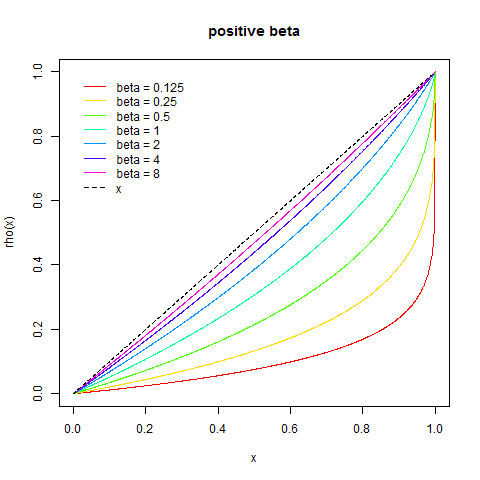
\includegraphics[width=0.6\textwidth]{fig/yule-beta.png}
	\end{center}
	\caption{Yule過程の解}\label{fig:Yule過程の解}
\end{figure} %}

\begin{todo}[今後の予定]\label{todo:今後の予定} %{
	メモ
	\begin{description} %{
		\item[2015-01-26] $\rho(\beta|x)$と$\CDF$(累積確率密度分布)との関係
		を調べる。少なくとも、$\rho(\beta|1)=\CDF(1)$となる。
		\item[2015-01-26] $\rho(\beta|-)$の逆関数を求める。
		$\rho(\beta|-):[0,1]\to[0,1]$は$1:1$になっているので、Lagrangeの定理を
		使って逆関数が求められる。
		\item[2015-01-26] $\rho(\beta|x)$の$x$についての解析接続を調べる。
		今のところ、優先順位は低い。
		\item[2015-01-25] $\beta\to\infty$の被積分関数の局在化によって説明する。
		\begin{description} %{
			\item[2015-01-26] 終了
		\end{description} %}
		\item[2015-01-25] ジーナスの確率分布$\rho(t,x)$ではなく分布そのもの
		$\nu(t,x)$を扱うことができないだろうか?
	\end{description} %}
	\EOP
\end{todo} %todo:今後の予定}
\subsection{微分方程式の解}\label{s2:微分方程式の解} %{
微分方程式\eqref{eq:diff-rho}をもう少し詳しく見る。

\subsubsection{線形の微分方程式}\label{s3:線形の微分方程式} %{
ゲージ変換を明示するために$\fukuso\pplr{x}$係数の$N$次元ベクトルで考える。

行列$A(x)\in M_N\plra{\fukuso\pplr{x}}$とベクトル$F(x)\in \fukuso\pplr{x}^N$
を固定して、次の微分方程式を考える。
\begin{equation*}\label{eq:diff-gen}
	\clD_A\phi(x) = F(x)
	\quad\text{where}\quad \clD_A\psi(x) := \plrg{\partial_x + A(x)}\psi(x)
	\quad\text{for all } \psi(x)\in\fukuso\pplr{x}^N
\end{equation*}
任意の$U(x)\in \GL_N\plra{\fukuso\pplr{x}}$と$\phi\in\fukuso\pplr{x}^N$に
対して次のゲージ変換が成り立つ。
\begin{equation*}
	\clD_A\phi(x) = \clD_AUU^{-1}\phi(x) = U\clD_{\clD_AU}U^{-1}\phi(x)
\end{equation*}
ここで、$\clD_AU$は次のように定義する。
\begin{equation*}
	\clD_AU(x) := U^{-1}(x)\plrg{\partial_x + A(x)}U(x)
	\quad\text{for all } U(x)\in \GL_N\plra{\fukuso\pplr{x}}
\end{equation*}
したがって、$D_AG=0$となる$G(x)\in \GL_N\plra{\fukuso\pplr{x}}$が求まると、
微分方程式\eqref{eq:diff-gen}の解$\phi$が次のように求まる。
\begin{equation*}
	\phi(x, y) = G(x)\int_y^x dz G^{-1}(z)F(z)
	\implies \plrgg{\partial_x + A(x)}\phi(x, y) = F(x)
\end{equation*}
そのような$G$があれば、次の式が成り立つ。
\begin{equation*}
	D_AG(x) = 0 \iff 
	A(x) = - \plrg{\partial_xG(x)}G^{-1}(x) = G(x)\partial_xG^{-1}(x)
\end{equation*}

$N=1$の場合は、ある$0<r\in\jitu$があって、$A(x)$が$\Ballx{x_0}{r}$で正則で
あれば、任意の$x\in\Ballx{x_0}{r}$に対して次のように書ける。
\begin{equation*}
	G(x) := G(x, x_0) = \exp\plra{- \int_{x_0}^x dzA(z)}
	\quad\text{for all } x\in\Ballx{x_0}{r}
	\quad\text{when } N = 1 
\end{equation*}
%s3:線形の微分方程式}
\subsubsection{微分方程式の解}\label{s3:微分方程式の解} %{
微分方程式\eqref{eq:diff-rho}を前節\ref{s3:線形の微分方程式}の筋書きに
添って解く。

\eqref{eq:diff-rho}の両辺を$\beta x(1 - x)$で割って次のように書き直すと、
\begin{equation}\label{eq:diff-rho-1}
	\plra{\partial_x + \frac{\beta}{x(1 - x)}}\rho(x) = \frac{\beta}{1 - x}
\end{equation}
$\frac{\beta}{x(1 - x)}$がゲージ場になることがわかる。そこで、$A$を
次のようにおき、
\begin{equation*}
	A(x) := \frac{\beta}{x(1 - x)}
\end{equation*}
\eqref{eq:diff-rho-1}の右辺が$xA(x)$と書けることに注意すると、
\eqref{eq:diff-rho-1}は次のように書け、
\begin{equation*}
	\plrg{\partial_x + A(x)}\rho(x) = xA(x)
\end{equation*}
その解$\rho(\beta|x,y)$は次のように書ける。
\begin{equation}\begin{split}\label{eq:rho-int-a}
	\rho(\beta|x,y) &= \exp\plra{- \int_{x_0}^x ds A(s)}
		\int_y^x dz \exp\plra{\int_{x_0}^z ds A(s)}zA(z) \\
	&= \exp\plra{- \int_{x_0}^x ds A(s)}
		\int_y^x dz \plra{\partial_z\exp\plra{\int_{x_0}^z ds A(s)}}z \\
\end{split}\end{equation}
そして、ゲージ場の積分は次のようになり、
\begin{equation*}
	\int_{x_0}^z ds A(s) = \int_{x_0}^z ds \frac{\beta}{x(1 - x)} 
	= \beta\ln\frac{\sigma(x)}{\sigma(x_0)}
\end{equation*}
解は次の形にまとまる。
\begin{equation*}
	\rho(\beta|x,y) = \int_{z=y}^x d\plra{\frac{\sigma(z)}{\sigma(x)}}^\beta z
\end{equation*}
ここで、$\sigma$は$(0,1,\infty)$を$(0,\infty,-1)$に移すM\"obius変換で、
次のように定義する。
\begin{equation*}
	\sigma(x) := \frac{x}{1 - x}
\end{equation*}
$\sigma(x)^\beta$は、$x=0$に$\beta$次のゼロ点、$x=1$に$\beta$次の発散点を
持つ。このことは、$D_\beta$の特異点が、確定特異点の$\set{0,1}$だけに
なっていることを反映している。任意の$0<\beta$に対して$x=0$で正則となることを
要請すると、$x=0$で$1/\sigma(x)$から生じる発散を避けるために、積分の始点$y$
が$0$に定まる。
\begin{equation}\label{eq:rho-int-1}
	\rho(\beta|x) := \rho(\beta|x,0) 
	= \int_{z=0}^x d\plra{\frac{\sigma(z)}{\sigma(x)}}^\beta z
\end{equation}
この解は次の性質を満たす。

\begin{description} %{
	\item[ベータ関数] 任意の$x\in\jitu$に対して$\rho(0|x)=0$だから、
	$0<\beta$の場合を考える。この時、\eqref{eq:rho-int-1}の積分変数を
	次のように変換していく。
	\begin{alignat*}{2}
		\rho(\beta|x) 
		&= \int_0^1 ds^\beta \sigma^{-1}\plrg{\sigma(x)s}
		&\quad&\text{// } s = \frac{\sigma(z)}{\sigma(x)} \\
		&= \beta x\int_0^1 ds \frac{s^\beta}{1 - x(1 - s)} \\
		&= \beta x\int_0^1 dt \frac{(1 - t)^\beta}{1 - xt}
		&\quad&\text{// } t = 1 - s
	\end{alignat*}
	この式では$\rho(0|x)=0$となるから、$\beta=0$の時も成り立ち、
	\begin{equation}\label{eq:rho-int-beta}
		\rho(\beta|x) = \beta x\int_0^1 dt \frac{(1 - t)^\beta}{1 - xt}
		\quad\text{for all } x < 1,\; 0 \le \beta
	\end{equation}
	原点近傍で次の級数展開が成り立つ。
	\begin{equation}\label{eq:rho-beta}
		\rho(\beta|x) = \beta x\sum_{n\in\sizen} x^nB(n + 1, \beta + 1)
		\quad\text{for all } |x| < 1 ,\; 0 \le \beta
	\end{equation}
	%
	\item[$x=0$の近傍] $x=0$近傍の様子は、級数展開\eqref{eq:rho-tay-beta}
	によってわかる。
	%
	\item[$x=1$の近傍] 積分表示\eqref{eq:rho-int-beta}から、$\rho(\beta|1)$が
	次のようになることがわかる。
	\begin{equation*}
		\rho(\beta|1) = \beta\int_0^1 dt (1 - t)^{\beta - 1}
		= \begin{cases}
			0, &\text{ if } \beta = 0 \\
			1, &\text{ otherwise } \\
		\end{cases}
	\end{equation*}
	また、\eqref{eq:rho-int-beta}を次のように書き換えると、
	\begin{equation*}
		\rho(\beta|x) = - \beta\int_{t=0}^1 d\plrg{\ln(1 - xt)}(1 - t)^\beta
	\end{equation*}
	任意の$n\in\sizen_+$に対して次の式を得る。
	\begin{equation*}
		\partial_x^n\rho(\beta|x) = \beta\int_{t=0}^1 
			d\plra{\frac{t}{1 - xt}}^n(1 - t)^\beta
	\end{equation*}
	この式を部分積分すると、$\partial_x^n\rho(\beta|x=1)$が次のようになること
	がわかる。
	\begin{equation*}\begin{split}
		\partial_x^n\rho(\beta|x=1)
		&= \beta \lim_{t\to1} t(1 - t)^{\beta - n}
			+ \beta^2\int_0^1 dt t^n(1 - t)^{\beta - n - 1} \\
		&= \begin{cases}
			B(n + 1, \beta - n), &\text{ if } n < \beta \\
			\infty, &\text{ otherwise } \\
		\end{cases}
	\end{split}\end{equation*}
	%
	\item[$\beta=0$の極限] $\beta=0$の時は、任意の$x\in\jitu$に対して
	$\rho(0|x)=0$となる。一方、任意の$0<\beta$で$\rho(\beta|1)=1$だから、
	$\lim_{\beta\to0+0}\rho(\beta|1)\neq\rho(0|1)$となって、$\rho(\beta|x)$は
	$\beta$について$0$で不連続になる。
	%
	\item[$\beta=\infty$の極限] 積分表示\eqref{eq:rho-int-beta}で、$\beta$が
	無限大に近づくと、被積分関数が局在化する。
	\begin{equation*}
		\lim_{\beta\to\infty}(1 - t)^\beta = \begin{cases}
			1, &\text{ if } t = 0 \\
			0, &\text{ otherwise } \\
		\end{cases}
	\end{equation*}
	このことは、部分積分を使って、次のように表され、
	\begin{equation*}\begin{split}
		\rho(\beta|x) &= \beta\int_0^1 dt\frac{(1 - t)^\beta}{1 - xt}
		= - \frac{\beta x}{\beta + 1}\blra{\frac{(1 - t)^{\beta + 1}}{1 - xt}}
			+ \frac{\beta x}{\beta + 1}\int_0^1 dt (1 - t)^{\beta + 1}
			\partial_x\frac{t}{1 -xt} \\
		&= \frac{\beta x}{\beta + 1} + \bigO\frac{x^2}{\beta}
	\end{split}\end{equation*}
	任意の$0\le x\le 1$で$\rho(\infty|x) = x$となることがわかる。
	この$\beta\to\infty$の漸近形は、固定した$x$と大きな$y$に対して成り立つ
	ベータ関数の近似$B(x,y)\sim \Gamma(x)y^{-x}$を\eqref{eq:rho-beta}に適用
	しても得られる。
	\begin{equation*}
		\rho(\beta|x) = \beta\sum_{n\in\sizen} B(n + 1, \beta + 1)x^{n+1}
		\xto{\beta\to\infty} \sum_{n\in\sizen}\frac{n!x^{n + 1}}{\beta^n}
	\end{equation*}
\end{description} %}
%s3:微分方程式の解}
%s2:微分方程式の解}
%s1:Yule過程}

\section{消滅付きのYule過程}\label{s1:消滅付きのYule過程} %{

\begin{todo}[パラメータの変更]\label{todo:パラメータの変更} %{
	$p_\del$から$p_\dup$に変更する。
\begin{procedure}\label{pro:消滅付きのYule過程その二}
	任意の時刻$t\in\sizen_+$で、
	\begin{enumerate} %{
		\item 確率$p_\new(t)$で新規ジーナスを作り、そのジーナスに新規スピシーズ
		を追加する。
		\item 確率$p_\new(t)^c$で既存のスピシーズからランダムに一つ選びだし、
		\begin{enumerate} %{
			\item 確率$p_\dup(t)$で、そのスピシーズの属するジーナスに
			新規スピシーズを追加し、
			\item 確率$p_\dup(t)^c$で、そのスピシーズを削除する。
		\end{enumerate} %}
	\end{enumerate} %}
	ここで、任意の確率$p$に対して$p^c:=1-p$と定義する。
	\EOP
\end{procedure}

\end{todo} %todo:パラメータの変更}

\begin{procedure}\label{pro:消滅付きのYule過程}
	任意の時刻$t\in\sizen_+$で、
	\begin{enumerate} %{
		\item 確率$p_\del(t)$で既存のスピシーズからランダムに一つ選びだし、
		そのスピシーズを削除する。
		\item 確率$p_\del(t)^cp_\new(t)$で新規ジーナスを作り、そのジーナスに
		新規スピシーズを追加する。
		\item 確率$p_\del(t)^cp_\new(t)^c$で既存のスピシーズをランダムに選び、
		そのスピシーズの属するジーナスに新規スピシーズを追加する。
	\end{enumerate} %}
	ここで、任意の確率$p$に対して$p^c:=1-p$と定義する。
	\EOP
\end{procedure}

時刻$t$での関数$\nu_n(t),\;\nu(t),\;\mu(t)$を次のように定義する。
\begin{itemize} %{
	\item 任意の$n\in\sizen$に対して$\nu_n(t)$をスピシーズを$n$個持つジーナス
	の数とする。
	\item $\nu(t)$をジーナスの総数とする。任意の時刻$t$で
	$\nu(t)=\sum_{n\in\sizen}\nu_n(t)$が成り立つ。
	\item $\mu(t)$をスピシーズの総数とする。任意の時刻$t$で
	$\mu(t)=\sum_{n\in\sizen}n\nu_n(t)$が成り立つ。
\end{itemize} %}

保持するスピシーズの数をジーナスの状態とみなすと、ジーナスの状態変化は
次の状態遷移図で表すことができる。
\begin{equation*}\xymatrix@C=12ex{
	& \ar[d]_{p_\del^cp_\new} \\
	0
	& 1 \ar[r]^{p_\del^cp_\new^c\cfrac{1}{\mu}} 
		\ar@<1ex>[l]^{p_\del\cfrac{1}{\mu}}
	& 2 \ar[r]^{p_\del^cp_\new^c\cfrac{2}{\mu}} 
		\ar@<1ex>[l]^{p_\del\cfrac{2}{\mu}} 
	& 3 \ar[r]^{p_\del^cp_\new^c\cfrac{3}{\mu}} 
		\ar@<1ex>[l]^{p_\del\cfrac{3}{\mu}} 
	& \cdots \ar@<1ex>[l]^{p_\del\cfrac{4}{\mu}}
}\end{equation*}
$\nu_n(t)$は次の漸化式を満たす。
\begin{equation}\label{eq:delta-nud}\begin{split}
	\delta\nu_0(t+1) &= p_\del(t)\cfrac{1}{\mu(t)}\nu_1(t) \\
	\delta\nu_1(t+1) &= p_\new(t)
	- \plrgg{p_\del(t) + q(t)}\cfrac{1}{\mu(t)}\nu_1(t)
	+ p_\del(t)\cfrac{2}{\mu(t)}\nu_2(t) \\
	\delta\nu_{n+1}(t+1)
	&= q(t)\cfrac{n}{t}\nu_n(t) 
	- \plrgg{p_\del(t) + q(t)}\cfrac{n+1}{\mu(t)}\nu_{n+1}(t) 
	+ p_\del(t)\cfrac{n+2}{\mu(t)}\nu_{n+2}(t)
\end{split}\end{equation}
ここで、$q(t)$は次のように定義する。
\begin{equation*}
	q(t) := p_\del(t)^cp_\new(t)^c
\end{equation*}
ここで、$\nu_n(t)$の生成関数$\nu(t,x)$を次のように定義すると、
\begin{equation}\begin{split}\label{eq:def-nu-1}
	\nu(t,x) := \sum_{n\in\sizen_+}\nu_n(t)x^n
\end{split}\end{equation}
漸化式\eqref{eq:delta-nud}は次の微分方程式で書き直すことができる。
\begin{equation}\label{eq:delta-nud-x}
	\delta\nu(t, x) = p_\new(t)x + \frac{q(t)}{\mu(t)}
	\plra{x - \frac{p_\del(t)}{q(t)}}\plra{x - 1}\partial_x\nu(t, x)
\end{equation}
$\nu(t)$と$\mu(t)$は、$\nu(t,x)$を用いて次のように書け、
\begin{equation}\label{eq:nud-delta}
	\nu(t) = \nu(t,1),\quad \mu(t) = \partial_x\nu(t, x = 1)
\end{equation}
それらの時間変化は次のようになる。
\begin{equation*}
	\delta\nu(t) = p_\new(t),\quad \delta\mu(t) = \begin{cases}
		0, &\text{ if } p_\del(t) = q(t) \\
		p_\new(t) + q(t) - p_\del(t), &\text{ otherwise } \\
	\end{cases}
\end{equation*}
時刻$t$でのジーナスの確率分布$\rho(t,x)$を次のように定義すると、
\begin{equation}\label{eq:def-rhod-1}
	\rho(t,x) := \frac{\nu(t,x)}{\nu(t)}
\end{equation}
\eqref{eq:nud-delta}を使って、\eqref{eq:delta-nud-x}は次のように書ける。
\begin{equation}\label{eq:exact-rhod}
	\rho(t+1,x) + \frac{\nu(t)}{p_\new(t)}\delta\rho(t,x) 
	= x + \frac{\nu(t)}{p_\new(t)}\frac{q(t)}{\mu(t)}
	\plra{x - \frac{p_\del(t)}{q(t)}}(x - 1)\partial_x\rho(t,x)
\end{equation}
ここで、時刻が無限大の極限で次の条件が成り立つと仮定する。
\begin{enumerate}\label{item:d-stable} %{
	\item\label{item:d-lhs} 次の式が成り立つ。
	\begin{equation*}
		\lim_{t\to\infty}\frac{\nu(t)}{p_\new(t)}\delta\rho(t,x) = 0
	\end{equation*}
	%
	\item\label{item:d-beta} ある$0<\beta\in\jitu\cup\set{\infty}$があって、
	次の式が成り立つ。
	\begin{equation*}\label{eq:d-beta}
		\lim_{t\to\infty}\frac{\nu(t)}{p_\new(t)}\frac{q(t)}{\mu(t)} 
		= \frac{1}{\beta}
	\end{equation*}
	%
	\item\label{item:d-gamma} ある$0\le\gamma\in\jitu$があって、
	次の式が成り立つ。
	\begin{equation*}\label{eq:d-gamma}
		\lim_{t\to\infty}\frac{p_\del(t)}{q(t)} = \gamma
	\end{equation*}
\end{enumerate} %}
条件\ref{item:d-lhs}は、次のように、ジーナスの確率分布が定常状態に収束する
ための十分条件になっている。
\begin{equation*}
	\delta\rho(t,x) = \frac{p_\new(t)}{\nu(t)}\frac{\nu(t)}{p_\new(t)}\delta\rho(t,x)
	\le \frac{\nu(t)}{p_\new(t)}\delta\rho(t,x)
	\quad\because\; \frac{p_\new(t)}{\nu(t)}\le 1 \quad\text{for all } 1\le t
\end{equation*}
これらの条件が成り立つと仮定し、時刻無限大の極限値を次のようにおくと、
\begin{equation*}
	\rho(x) := \lim_{t\to\infty}\rho(t,x)
\end{equation*}
微分方程式\eqref{eq:delta-nud-x}の時刻が無限大の極限は次のようになる。
\begin{equation}\label{eq:diff-rhod}
	\rho(x) = x + \frac{1}{\beta}(x - \gamma)(x - 1)\partial_x\rho(x)
\end{equation}
$(\gamma,1,\infty)$を$(0,\infty,-1)$に移すM\"obius変換$\sigma(\gamma|-)$
を次のように定義すると、
\begin{equation}\label{eq:rhod-mobius}
	\sigma(\gamma|x) := \frac{x - \gamma}{1 - x}
\end{equation}
\eqref{eq:diff-rhod}は次のように書ける\eqref{eq:rhod-mobius-diff}。
\begin{equation*}
	\plra{\partial_x 
		+ \frac{\beta}{1 - \gamma}\partial_x\ln\sigma(\gamma|x)}\rho(x)
	= \frac{\beta x}{1 - \gamma}\partial_x\ln\sigma(\gamma|x)
\end{equation*}
左辺の微分演算子は、$x=\gamma,\,1$のみに確定特異点を持ち、右辺の関数も
$x=\gamma,\,1$のみに$1$次の極を持つ。
この微分方程式の一般解$\rho(\beta,\gamma|-,-)$は次のように書くことができる。
\begin{equation}\label{eq:rhod-y}
	\rho(\beta,\gamma|x,y) = \int_{z=y}^x d \plra{\frac{\sigma(\gamma|z)}
		{\sigma(\gamma|x)}}^{\frac{\beta}{1 - \gamma}}z
\end{equation}
この式で、積分定数$y$を決めると、解$\rho(\beta,\gamma|x)$が定まる。
$\rho(\beta,\gamma|x)$が$x\in(0,1)$で正則になるように、次のようにして$y$を
定める。
\begin{description} %{
	\item[$0\le\gamma<1$の時] $\sigma(\gamma|x)^{\frac{\beta}{1 - \gamma}}$
	は$x=\gamma$で$0$、$x=1$で$\infty$となるので、$y=\gamma$と定める。
	\begin{equation*}
		\lim_{x\to x_*}\rho(\beta,\gamma|x,0) = \lim_{x\to x_*}\frac
			{x\partial_x\sigma(\beta,\gamma|x)^{\frac{\beta}{1 - \gamma}}}
			{\partial_x\sigma(\beta,\gamma|x)^{\frac{\beta}{1 - \gamma}}}
		= x_* \quad\text{for } x_* = 0,1
	\end{equation*}
	\item[$1<\gamma$の時] $\sigma(\gamma|x)^{\frac{\beta}{1 - \gamma}}$
	は$x=\gamma$で$\infty$、$x=1$で$0$となるので、$y=1$と定める。
	\begin{equation*}
		\lim_{x\to 1}\rho(\beta,\gamma|x,1) = \lim_{x\to 1}\frac
			{x\partial_x\sigma(\beta,\gamma|x)^{\frac{\beta}{1 - \gamma}}}
			{\partial_x\sigma(\beta,\gamma|x)^{\frac{\beta}{1 - \gamma}}}
		= 1
	\end{equation*}
\end{description} %}
まとめると、次のようになるが、
\begin{equation*}
		\rho(\beta,\gamma|x) = \begin{cases}
			\rho(\beta,\gamma|x,\gamma), &\text{ if } 0\le\gamma<1 \\
			\rho(\beta,\gamma|x,1), &\text{ if } 1<\gamma \\
		\end{cases}
\end{equation*}
次の式\eqref{eq:rhod-rec}を使って、計算しやすい方で計算すれば良い。
\begin{equation}\label{eq:rhod-1}
	\rho(\beta,\gamma|x) = \gamma\rho\plra{
		\frac{\beta}{\gamma},\frac{1}{\gamma} | \frac{x}{\gamma}}
	\quad\text{for all } 1 < \gamma
\end{equation}
また、解\eqref{eq:rhod-1}の$\gamma=1$の極限は、上からと下からの極限が一致し
\eqref{eq:rhod-one}、次のようになる。
\begin{equation*}
	\rho(\beta,1|x) = \int_{z=1}^x d\plra{
		\exp\plra{- \beta\plra{\frac{1}{1 - z} - \frac{1}{1 - x}}}}z
\end{equation*}
\subsection{計算のメモ}\label{s2:計算のメモ} %{
\subsubsection{ゲージ場のM\"obius変換}\label{s3:ゲージ場のMobius変換} %{
M\"obius変換\eqref{eq:rhod-mobius}の性質を書いておく。
\begin{description} %{
	\item[微分]	\eqref{eq:rhod-mobius}の微分は次のようになり、
	\begin{equation*}
		\partial_x\sigma(\gamma|x) = \frac{1 - \gamma}{(1 - x)^2}
	\end{equation*}
	次の式が成り立つ。
	\begin{equation}\label{eq:rhod-mobius-diff}
		\partial_x\ln\sigma(\gamma|x) = \frac{1 - \gamma}{(x - \gamma)(1 - x)}
	\end{equation}
	%
	\item[逆数] 次の式が成り立つ。
	\begin{equation}\label{eq:rhod-mobius-rec}
		\sigma(\gamma|\gamma x) = \sigma(\frac{1}{\gamma}|x)^{-1}
	\end{equation}
	%
	\item[逆変換] \eqref{eq:rhod-mobius}を行列で表すと次のようになり、
	\begin{equation*}
		\sigma(\gamma|x) = \begin{pmatrix}
			1 & -\gamma \\ -1 & 1
		\end{pmatrix}\begin{pmatrix}
			x \\\hline 1
		\end{pmatrix} = \frac{x - \gamma}{1 - x}
	\end{equation*}
	逆行列をとることで、逆変換$\sigma^{-1}(\gamma|-)$が次のように求まる。
	\begin{equation*}
		\sigma^{-1}(\gamma|x) = \plra{\frac{1}{1 - \gamma}\begin{pmatrix}
			1 & \gamma \\ 1 & 1
		\end{pmatrix}}\begin{pmatrix}
			x \\\hline 1
		\end{pmatrix} = \begin{pmatrix}
			1 & \gamma \\ 1 & 1
		\end{pmatrix}\begin{pmatrix}
			x \\\hline 1
		\end{pmatrix} = \frac{x + \gamma}{x + 1}
	\end{equation*}
	ここで、逆行列の行列式による因子$1 / (1 - \gamma)$は、M\"obius変換には
	効かないことに注意する。
\end{description} %}
%s3:ゲージ場のMobius変換}
\subsubsection{$\rho$の$\gamma$反転}\label{s3:rhoのgamma反転} %{
M\"obius変換の逆数について成り立つ式\eqref{eq:rhod-mobius-rec}を使うと、
次の式が得られる。
\begin{alignat*}{2}
	\rho(\beta,\gamma|x,1) 
	&= \int_{z=1}^x d\plra{\frac{\sigma(\gamma|z)}{\sigma(\gamma|x)}}
		^{\frac{\beta}{1 - \gamma}}z \\
	&= \int_{z=1}^x d\plra{\frac
		{\sigma\plra{\frac{1}{\gamma}|\frac{z}{\gamma}}}
		{\sigma\plra{\frac{1}{\gamma}|\frac{x}{\gamma}}}}
		^{\frac{\beta}{\gamma}\frac{1}{1 - \frac{1}{\gamma}}}z 
		&\quad&\text{// } \eqref{eq:rhod-mobius-rec} \\
 &= \gamma \int_{w=\frac{1}{\gamma}}^{\frac{x}{\gamma}} d\plra{\frac
		{\sigma\plra{\frac{1}{\gamma}|w}}
		{\sigma\plra{\frac{1}{\gamma}|\frac{x}{\gamma}}}}
		^{\frac{\beta}{\gamma}\frac{1}{1 - \frac{1}{\gamma}}}w
		&\quad&\text{// } w = \frac{z}{\gamma} \\
 &= \gamma \rho\plra{\frac{\beta}{\gamma},\frac{1}{\gamma}
		| \frac{x}{\gamma},\frac{1}{\gamma}}
\end{alignat*}
したがって、次の式が成り立つ。
\begin{equation}\label{eq:rhod-rec}
	\rho(\beta,\gamma|x) = \gamma\rho\plra{
		\frac{\beta}{\gamma},\frac{1}{\gamma} | \frac{x}{\gamma}}
	\quad\text{for all } 1 < \gamma
\end{equation}
%s3:s3:rhoのgamma反転}
\subsubsection{$\gamma\to1$の極限}\label{s3:gamma=1の極限} %{
解\eqref{eq:rhod-1}の$\gamma=1$の上からと下からの極限は、それぞれ次のように
なり、
\begin{equation}\label{eq:rhod-one}\begin{split}
	\lim_{\epsilon\to0}\rho(\beta, 1 - \epsilon | x)
	&= \lim_{\epsilon\to0}\rho(\beta, 1 - \epsilon|x, 1 - \epsilon) \\
	&= \lim_{\epsilon\to0}\int_{z = 1 - \epsilon}^x \plra{
		\frac{1 - \frac{\epsilon}{1 - z}}{1 - \frac{\epsilon}{1 - x}}}
		^ {\frac{\beta}{\epsilon}}z
	= \int_{z = 1}^x \plra{
		\frac{\exp\plra{- \frac{1}{1 - z}}}
		{\exp\plra{ - \frac{\epsilon}{1 - x}}}}^ \beta z \\
	\lim_{\epsilon\to0}\rho(\beta, 1 + \epsilon | x)
	&= \lim_{\epsilon\to0}\rho(\beta, 1 + \epsilon|x, 1) \\
	&= \lim_{\epsilon\to0}\int_{z = 1}^x \plra{
		\frac{1 + \frac{\epsilon}{1 - z}}{1 + \frac{\epsilon}{1 - x}}}
		^ {- \frac{\beta}{\epsilon}} z
	= \int_{z = 1}^x \plra{
		\frac{\exp\plra{- \frac{1}{1 - z}}}
		{\exp\plra{ - \frac{\epsilon}{1 - x}}}}^\beta z
\end{split}\end{equation}
両者が一致する。$0<\beta$として、この式を$x=0$近傍で展開すると、
次のようになる。
\begin{alignat*}{2}
	\rho(\beta,1|x) &= \int_{z=1}^x d\plra{
		\exp\plra{- \beta\plra{\frac{1}{1 - z} - \frac{1}{1 - x}}}} z \\
	&= \int_{w=\infty}^0 de^{- \beta w}
		\plra{1 - \frac{1}{w + \frac{1}{1 - x}}}
		&\quad&\text{// } w = \frac{1}{1 - z} - \frac{1}{1 - x} \\
 &= 1 - \beta\int_0^\infty dw e^{- \beta w}\frac{1 - x}{(1 - x)w + 1} \\
 &= 1 - \beta\sum_{n\in\sizen}\int_0^\infty dw e^{- \beta w}
		\frac{1 - x}{w + 1}\plra{\frac{wx}{w + 1}}^n 
		&\quad&\text{// } wx < w + 1 \\
 &= 1 - \beta\int_0^\infty \frac{dw}{w + 1}e^{- \beta w}
		+ \beta \sum_{n\in\sizen}x^{n + 1} \int_0^\infty
		\frac{dw w^n}{(w + 1)^{n + 2}} e^{- \beta w} \\
	&= \int_0^\infty \frac{dw}{(w + 1)^2}e^{- \beta w}
		+ \beta \sum_{n\in\sizen}x^{n + 1} \int_0^\infty
		\frac{dw}{(w + 1)^2} e^{- \beta w}\plra{\frac{w}{w + 1}}^n
\end{alignat*}
%s3:gamma=1の極限}
\subsubsection{原点近傍のTaylor展開}\label{s3:原点近傍のTaylor展開} %{
この節では、特に断らない限り$0<\gamma<1$とする。

$0\le b\in\jitu$を次のように定義すると、
\begin{equation*}
	b := \frac{\beta}{1 - \gamma}
\end{equation*}
\eqref{eq:rhod-y}から、解$\rho(\beta,\gamma|x)$は次のようになり、
\begin{alignat*}{2}
	\rho(\beta,\gamma|x) &= \int_{z=\gamma}^x 
		d\plra{\frac{\sigma(\gamma|z)}{\sigma(\gamma|x)}}^b z \\
	&= \int_{w=0}^1 dw^b\sigma^{-1}\plra{\gamma|\sigma(\gamma|x)w}
	&\quad&\text{// } w = \frac{\sigma(\gamma|z)}{\sigma(\gamma|x)} \\
	&= \int_{w=0}^1 dw^b
		\plra{1 - \frac{1 - \gamma}{\sigma(\gamma|x)w + 1}} \\
	&= 1 - (1 - \gamma)\int_{w=0}^1 \frac{dw^b}{\sigma(\gamma|x)w + 1}
\end{alignat*}
任意の$0<w,x,\gamma<1$に対して次のべき展開が成り立つから、
\begin{alignat*}{2}
	\frac{1}{\sigma(\gamma|x)w + 1} 
	&= \frac{1 - x}{(1 - \gamma w) - (1 - w)x} \\
	&= \frac{1 - x}{1 - \gamma w}\sum_{n\in\sizen}
		\plra{\frac{1 - w}{1 - \gamma w}x}^n 
	&\quad&\text{// } \frac{1 - w} {1 - \gamma w} x < 1 \\
	&= \frac{1}{1 - \gamma w}
		- \frac{(1 - \gamma)w}{(1 - \gamma w)^2}\sum_{n\in\sizen} x^{n + 1}
		\plra{\frac{1 - w}{1 - \gamma w}}^n
\end{alignat*}
次の式が得られる。
\begin{equation*}\begin{split}
	\rho(\beta,\gamma|x) 
	&= 1 - (1 - \gamma)\int_{w=0}^1 \frac{dw^b}{1 - \gamma w}
		+ (1 - \gamma)^2\sum_{n\in\sizen} x^{n + 1} \int_0^1 
		\frac{dw^b w}{(1 - \gamma w)^2}\plra{\frac{1 - w}{1 - \gamma w}}^n \\
	&= \gamma(1 - \gamma)\int_0^1 dw \frac{w^b}{(1 - \gamma w)^2}
		+ \beta(1 - \gamma)\sum_{n\in\sizen}x^{n + 1}\int_0^1 dw 
		\frac{w^b}{(1 - \gamma w)^2} \plra{\frac{1 - w}{1 - \gamma w}}^n \\
\end{split}\end{equation*}
べき展開の係数$\rho_n(\beta,\gamma)$を次のように定義し、
\begin{equation*}
	\rho(\beta,\gamma|x) = \sum_{n\in\sizen}x^n\rho_n(\beta,\gamma)
\end{equation*}
関数$R_n(\beta,\gamma)$を次のように定義すると、
\begin{equation*}
	R_n(\beta,\gamma) := (1 - \gamma)\int_0^1dz\frac{z^b}
		{(1 - \gamma z)^2}\plra{\frac{1 - z}{1 - \gamma z}}^n
\end{equation*}
係数は次のように書ける。
\begin{equation}\label{eq:rhod-taylor}
	\rho_0(\beta, \gamma) = \gamma R_0(\beta, \gamma)
	,\quad \rho_{n + 1}(\beta, \gamma) = \beta R_n(\beta, \gamma)
	\quad\text{for all } 0 < \gamma < 1
\end{equation}
$\gamma=0,\infty,1$の場合を計算すると、次のようになる。
\begin{description} %{
	\item[$\gamma=0$の時] $\rho_n(\beta,0)$は次のようになるが、
	\begin{equation*}
		\rho_0(\beta,0) = \lim_{\epsilon\to0}\epsilon R_0(\beta,\epsilon)
		,\quad \rho_{n+1}(\beta,0) = \beta\lim_{\epsilon\to0}R_n(\beta,\epsilon)
	\end{equation*}
	$R_n(\beta,0)$は次のようにベータ関数になり、
	\begin{equation*}
		R_n(\beta,0) = \int_0^1dzz^\beta(1 - z)^n = B(n + 1, \beta + 1)
	\end{equation*}
	$\rho_n(\beta,0)$は次のようになる。
	\begin{equation*}
		\rho_0(\beta,0) = 0
		,\quad \rho_{n+1}(\beta,0) = \beta B(n + 1, \beta + 1)
	\end{equation*}
	特に、$n=1$と大きな$n$に対しては次のようになる。
	\begin{equation*}
		\rho_1(\beta,0) = \frac{\beta}{\beta + 1}
		,\quad \rho_n(\beta,0) \sim \beta\Gamma(\beta + 1)n^{- (\beta + 1)}
		\quad\text{for } n\sim \infty
	\end{equation*}
	%
	\item[$\gamma=\infty$の時] $\rho_n(\beta,\infty)$は、
	\eqref{eq:rhod-1}から、次のようになるが、
	\begin{alignat*}{3}
		\rho_0(\beta,\infty|x)
		&= \lim_{\epsilon\to0}\frac{\rho_0(\epsilon\beta,\epsilon)}{\epsilon}
		&&= \lim_{\epsilon\to0}R_0(\epsilon\beta,\epsilon) \\
		\rho_{n+1}(\beta,\infty|x)
		&= \lim_{\epsilon\to0}\frac{\epsilon^{n+1}\rho_{n+1}(\epsilon\beta,\epsilon)}{\epsilon}
		&&= \beta\lim_{\epsilon\to0}\epsilon^{n+1}R_n(\epsilon\beta,\epsilon)
	\end{alignat*}
	$R_n(0,0)$は次のようになり、
	\begin{equation*}
		R_n(0,0) = \int_0^1dz(1 - z)^n = \frac{1}{n + 1}
	\end{equation*}
	$\rho_n(\beta,\infty)$は次のようになる。
	\begin{equation*}
		\rho_0(\beta,\infty) = 1 ,\quad \rho_{n+1}(\beta,\infty) = 0
	\end{equation*}
	%
	\item[$\gamma=1$の時] $\rho_n(\beta,1)$は次のようになるが、
	\begin{equation*}
		\rho_0(\beta,1) = \lim_{\epsilon\to0}(1 - \epsilon)R_0(\beta,1 - \epsilon)
		,\quad \rho_{n+1}(\beta,1) = \beta\lim_{\epsilon\to0}R_n(\beta, 1 - \epsilon)
	\end{equation*}
	$R_n(\beta,1-\epsilon)$は次のようになる。
	\begin{alignat*}{2}
		R_n(\beta,1-\epsilon) &= \epsilon\int_0^1 dz
			\frac{z^{\frac{\beta}{\epsilon}}}{\plrg{1 - (1 - \epsilon)z}^2}
			\plra{\frac{1 - z}{1 - (1 - \epsilon)z}}^n \\
		&= \epsilon^2\int_0^\infty dt \frac{e^{- (\beta + \epsilon)t}}
			{\plrg{1 - (1 - \epsilon)e^{- \epsilon t}}^2}
			\plra{\frac{1 - e^{- \epsilon t}}
			{1 - (1 - \epsilon)e^{- \epsilon t}}}^n
			&\quad&\text{// } t = - \frac{\ln z}{\epsilon}
	\end{alignat*}
	ここで、$A(\epsilon|t)$と$B(\epsilon|t)$を次のようにおくと、
	\begin{alignat*}{2}
		1 - (1 - \epsilon)e^{- \epsilon t} &= \epsilon A(\epsilon|t)
		,&\quad A(\epsilon|t) &:= \sum_{n\in\sizen}
			\frac{(- \epsilon t)^n}{n!}\plra{1 + \frac{t}{n + 1}} \\
		1 - e^{- \epsilon t} &= \epsilon tB(\epsilon|t) 
		,&\quad B(\epsilon|t)	&:= \sum_{n\in\sizen}
			\frac{(- \epsilon t)^n}{(n + 1)!}
	\end{alignat*}
	$R_n(\beta,1-\epsilon)$は次のように書ける。
	\begin{equation*}
		R_n(\beta,1-\epsilon) = \int_0^\infty dt 
		\frac{e^{- (\beta + \epsilon)t}}{A(\epsilon|t)^2}
		\plra{\frac{tB(\epsilon|t)}{A(\epsilon|t)}}^n
	\end{equation*}
	ここで、次の極限を成り立つと仮定すると、
	\begin{equation*}
		\lim_{\epsilon\to0} R_n(\beta,1-\epsilon) = \int_0^\infty dt 
			\frac{e^{- \beta t}}{A(0|t)^2}\plra{\frac{tB(0|t)}{A(0|t)}}^n
		= \int_0^\infty dt 
			\frac{e^{- \beta t}}{(t + 1)^2}\plra{\frac{t}{t + 1}}^n
	\end{equation*}
	$\rho_n(\beta,1)$は次のようになり、前節\ref{s3:gamma=1の極限}の結果が再現
	される。
	\begin{equation*}
		\rho_0(\beta,1) = \int_0^\infty dt \frac{e^{- \beta t}}{(t + 1)^2}
		,\quad \rho_{n+1}(\beta,1) = \beta\int_0^\infty dt 
			\frac{e^{- \beta t}}{(t + 1)^2}\plra{\frac{t}{t + 1}}^n
	\end{equation*}
	$\rho_0(\beta,1)$は次のように書き直せるが、
	\begin{equation*}\begin{split}
		\rho_0(\beta,1)
		= - \int_0^\infty dt e^{- \beta t}\partial_t\frac{1}{t + 1}
		= 1 - \beta\int_0^\infty \frac{dt}{t + 1}e^{- \beta t}
		= 1 - \beta e^\beta\int_1^\infty \frac{ds}{s}e^{- \beta s}
	\end{split}\end{equation*}
	最後の式の二項目は指数積分と呼ばれる関数\cite{Expon0:online}で、次の評価
	が成り立つ。
	\begin{equation*}
		\frac{1}{2}e^{- \beta}\ln\plra{1 + \frac{2}{\beta}}
		< \int_1^\infty \frac{ds}{s}e^{- \beta s}
		< e^{- \beta}\ln\plra{1 + \frac{1}{\beta}}
	\end{equation*}
	したがって、$\rho_0(\beta,1)$は次のように評価することができる。
	\begin{equation*}
		1 - \beta\ln\plra{1 + \frac{1}{\beta}}
		< \rho_0(\beta,1)
		< 1 - \frac{\beta}{2}\ln\plra{1 + \frac{2}{\beta}}
	\end{equation*}
\end{description} %}
%s3:原点近傍のTaylor展開}
%s2:計算のメモ}
%s1:消滅付きのYule過程}

\section{計算}\label{s1:計算} %{
\subsection{ベータ関数}\label{s2:ベータ関数} %{
$0<\Re x,\; 0<\Re y$に対してベータ関数$B(x,y)$は次のように定義される。
\begin{equation}\label{eq:Beta}
	B(x, y) := \int_0^1 \frac{dt}{t(1-t)}t^x(1-t)^y
	\quad\text{for all } 0<\Re x,\; 0<\Re y
\end{equation}

ベータ関数とガンマ関数は次の関係にある。
\begin{equation}
	B(x, y) = \frac{\Gamma(x)\Gamma(y)}{\Gamma(x+y)}
	\quad\text{for all } 0<\Re x,\; 0<\Re y
\end{equation}
\begin{proof} %{
	定義\eqref{eq:Beta}の積分変数を$s:=t/(1-t)$と変換すると、ガンマ関数の
	積分表示が現れる。
	\begin{alignat*}{2}
		B(x, y) &= \int_0^\infty\frac{ds}{s}\frac{s^x}{(1+s)^{x+y}}
		&\quad&\text{// } s := \frac{t}{1-t} \\
		&= \frac{1}{\Gamma(x+y)}\int_0^\infty\frac{ds}{s}s^x
		\int_0^\infty\frac{du}{u}u^{x+y}e^{-(1+s)u}
		&\quad&\text{// } \Gamma(x) = a^x\int_0^\infty\frac{dt}{t}t^xe^{-at} \\
		&= \frac{1}{\Gamma(x+y)}\int_0^\infty\frac{du}{u}u^{x+y}e^{-u}
		\int_0^\infty\frac{ds}{s}s^xe^{-su} \\
		&= \frac{\Gamma(x)}{\Gamma(x+y)}\int_0^\infty\frac{du}{u}u^ye^{-u} \\
		&= \frac{\Gamma(x)\Gamma(y)}{\Gamma(x+y)}
	\end{alignat*}
\end{proof} %}

定義\eqref{eq:Beta}の積分路を変形して、$y$の実部が負の場合に解析接続しよう。
$C$を図\ref{fig:ベータ関数の積分路その一}の積分路とすると、次の式が成り立つ。
\begin{equation*}
	B(x,y) = \frac{1}{1 - e^{-2\pi iy}}\int_C \frac{dt}{t(1 - t)}t^x(1 - t)^y
	\quad\text{for all } 0 < \Re x,\; 0 < \Re y,\; y\not\in\sei
\end{equation*}
ここで、複素平面の分岐切断は、$x\in\sei$の時は$(-\infty,1)$、$x\not\in\sei$
の時は$(0,1)$とする。

\begin{figure}[htbp] %{
	\begin{center}
		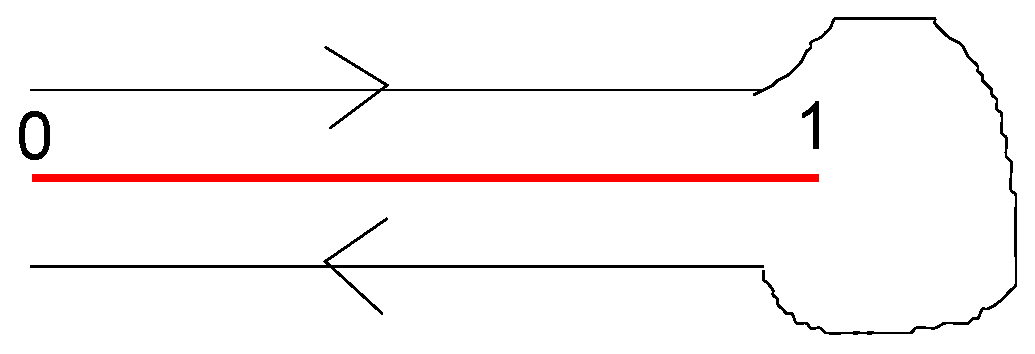
\includegraphics[width=0.3\textwidth]{fig/contour-2.eps}
	\end{center}
	\caption{ベータ関数の積分路その一}\label{fig:ベータ関数の積分路その一}
\end{figure} %}
%s2:ベータ関数}
\subsection{ベータ関数の和}\label{s2:ベータ関数の和} %{
$0<\Re a$かつ$0<\Re b$とすると、次の式が成り立ち、
\begin{equation*}
	\sum_{n\in\sizen}B(n + a, b)x^n 
	= \int_0^1 \frac{dt}{t(1 - t)}t^a(1 - t)^b \sum_{n\in\sizen}(tx)^n
	= \int_0^1 \frac{dt}{t(1 - t)}\frac{t^a(1 - t)^b}{1 - xt}
\end{equation*}
次の式が得られる。
\begin{equation*}\begin{split}
	\sum_{n\in\sizen}B(n + a, b) = B(a, b - 1) 
\end{split}\end{equation*}
%s2:ベータ関数の和}
\subsection{二項係数の計算}\label{s2:二項係数の計算} %{
任意の$0<k\in\jitu,\;x\in\Ballx{0}{1}$に対して次の式が成り立つ。
\begin{equation}\label{eq:分数の二項係数}
	(1 - x)^{-k} = \sum_{n\in\sizen}\frac{x^n\Gamma(k+n)}{n!\Gamma(k)}
	= \sum_{n\in\sizen}\frac{x^n}{(n + k)B(n + 1, k)}
\end{equation}
$k\in\fukuso$でも成り立つと思うが、その場合は解析接続が必要になる。
%s2:二項係数の計算}
%s1:計算}

\section{バックアップ}\label{s1:バックアップ} %{
\begin{description}\setlength{\itemsep}{-1mm} %{
	%
	\item[級数展開] M\"obius変換を明示的に示す級数展開を導く。
	\eqref{eq:rho-int-1}の積分変数を次のように変換する。
	\begin{alignat*}{2}
		\rho(\beta|x) 
		&= \sigma(x)^{-\beta}\int_0^{\sigma(x)} d(s^\beta)\sigma^{-1}(s)
		&\quad&\text{// } s = \sigma(z),\;\sigma^{-1}(s) = \frac{s}{1 + s} \\
		&= \sigma(x)^{-\beta}\int_0^{\sigma(x)^\beta} dt\sigma^{-1}(t^{\frac{1}{\beta}})
		&\quad&\text{// } t = s^\beta
	\end{alignat*}
	$\sigma^{-1}(t^{1/\beta})$を$t^{1/\beta}=0$近傍でべき展開するが、$x$の値に
	よって場合分けする必要がある。
	\begin{description}\setlength{\itemsep}{-1mm} %{
		\item[$x\le 1/2$の時] この時は、$\sigma(x)\le 1$となり、被積分変数$t$が
		$|t|<1$となり、次のようにべき展開できる。
		\begin{equation*}
			\rho(\beta|x) = \sigma(x)^{-\beta}\int_0^{\sigma(x)^\beta} dt 
				t^{\frac{1}{\beta}}\sum_{n\in\sizen} \plra{- t^{\frac{1}{\beta}}}
			= \beta \sum_{n\in\sizen} (-)^n\frac{\sigma(x)^{n + 1}}{\beta + n + 1}
		\end{equation*}
		%
		\item[$1/2< x$の時] この時は、$1<\sigma(x)$となり、被積分変数$t$が
		$|t|<1$ではなくなり、積分範囲を分割する必要がある。
		\begin{equation*}\begin{split}
			\rho(\beta|x) 
			= \sigma(x)^{-\beta}\plra{\int_0^1 + \int_1^{\sigma(x)^\beta}} dt 
			\sigma^{-1}\plra{t^{\frac{1}{\beta}}}
		\end{split}\end{equation*}
		一つ目の積分は$x\le1/2$の場合と同じだが、二つ目の積分はべき展開が異なる。
		\begin{equation*}\begin{split}
			\sigma(x)^{-\beta}\int_1^{\sigma(x)^\beta}dt
				\sigma^{-1}\plra{t^{\frac{1}{\beta}}}
			&= \sigma(x)^{-\beta}\int_1^{\sigma(x)^\beta}dt
				\sum_{n\in\sizen}\plra{- t^{- \frac{1}{\beta}}}^n \\
			&= - \beta\sum_{n\in\sizen}(-)^n
				\frac{\sigma(x)^{- \beta} - \sigma(x)^{- n}}{\beta - n}
		\end{split}\end{equation*}
		$\beta\in\sizen$の場合、和の中に不定な項が現れるが、それは次の極限を
		とるものとする。
		\begin{equation*}
			\lim_{\beta\to n}\frac{\sigma(x)^{- \beta} - \sigma(x)^{- n}}{\beta - n}
			= - \lim_{\beta\to n}\sigma(x)^{- \beta}\ln\sigma(x)
			= - \frac{\ln\sigma(x)}{\sigma(x)^n}
		\end{equation*}
	\end{description} %}
	以上をまとめると、次の級数展開が得られる。
	\begin{equation}\label{eq:rho-int-mobius}
		\rho(\beta|x) = \beta\sum_{n\in\sizen}(-)^n\begin{cases}
			\cfrac{\sigma(x)^{n + 1}}{\beta + n + 1}
			, &\text{ if } |x| < \frac{1}{2} \\
			\cfrac{1}{\beta + n + 1} 
			- \cfrac{\sigma(x)^{- \beta} - \sigma(x)^{- n}}{\beta - n}
			, &\text{ otherwise } \\
		\end{cases}
	\end{equation}
\end{description} %}

\subsection{分岐を持つ複素積分} % (fold)
\label{sub:分岐を持つ複素積分}
単位円上の積分$\oint_{|z|=1}dzz^{\frac{1}{2}}$を考える。
円座標を使って計算すると次のようになる。
\begin{alignat*}{2}
	\oint_{|z|=1}dzz^{\frac{1}{2}}
	&= i\int_0^{2\pi} d\theta \exp\plra{\frac{3i}{2}\theta}
	&\quad&\text{// } z = \exp\plra{i\theta} \\
	&= \frac{2}{3}\blra{\exp\plra{\frac{3i}{2}\theta}}_{\theta=0}^{2\pi}
	= - \frac{4}{3}
\end{alignat*}
積分路の組み合わせを使って計算してみよう。図\ref{fig:積分路その一}のように、
$C_1$を$|z|=1$の反時計回りの円周、$C_\epsilon$を$|z|=\epsilon<1$の時計回りの円周、
$L_+$を$\epsilon$から$1$への実軸上の直線、$L_-$を$1$から$\epsilon$への実軸上の直線とし、
それらを繋げた閉路を$\Gamma$とする。
\begin{equation*}
	\oint_\Gamma = \int_{C_1} + \int_{L_-} + \int_{C_\epsilon} + \int_{L_+}
\end{equation*}
$dzz^{\frac{1}{2}}$の分岐を正の実軸にとると、$\Gamma$の内部には$dzz^{\frac{1}{2}}$の極と
分岐が無いので、$\oint_\Gamma dzz^{\frac{1}{2}}=0$となり、
$\lim_{\epsilon\to0}\int_{C_\epsilon}dzz^{\frac{1}{2}}=0$だから、次の式が成り立つ。
\begin{equation}\begin{split}\label{eq:branch-1}
	\int_{C_1}dzz^{\frac{1}{2}} 
	&= - \lim_{\epsilon\to0}\plra{\int_{L_-} + \int_{L_+}}dzz^{\frac{1}{2}} \\
	&= - \int_1^0 dze^{\pi i}z^{\frac{1}{2}} - \int_0^1 dzz^{\frac{1}{2}}
	= \int_1^0 dzz^{\frac{1}{2}} - \int_0^1 dzz^{\frac{1}{2}} = - \frac{4}{3}
\end{split}\end{equation}

\begin{figure}[htbp] %{
	\begin{center}
		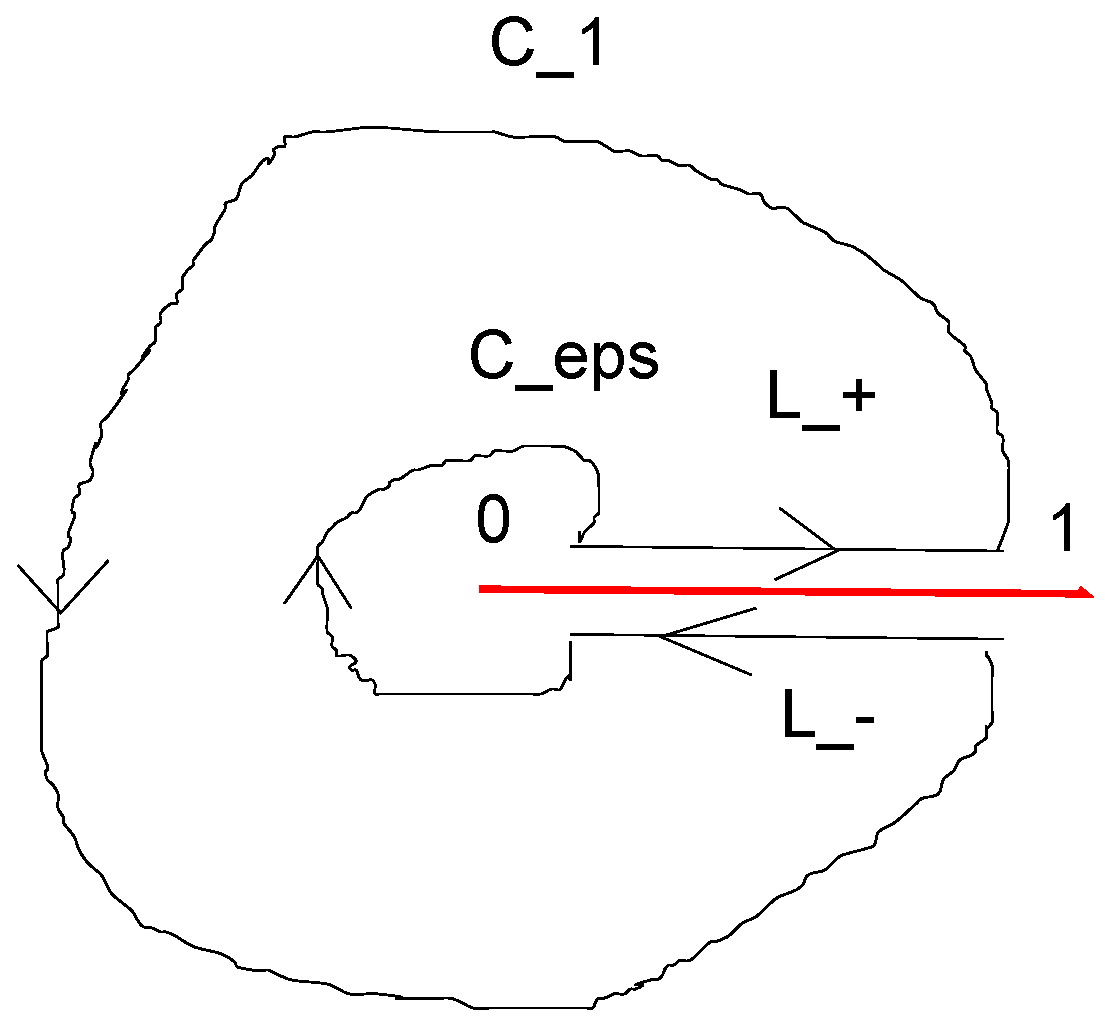
\includegraphics[width=0.3\textwidth]{fig/contour-1.eps}
	\end{center}
	\caption{積分路その一}\label{fig:積分路その一}
\end{figure} %}

$\int_1^z$の積分路によって$\ln z$の多意性$\ln z+2n\pi i$を表すことができる。
積分路が原点の周りを時計回りに一周する毎に、$2\pi i$ずつ$\ln z$に加算されて
いく。逆に、多意性を取り除くために、複素平面から原点を取り除き、原点から
無限遠点までハサミで切断した空間$K_0$を考え、$\int_1^z$の積分路を$K_0$内に
限定したものを$\ln z$と定義し、$z^a$を$e^{a\ln z}$によって定義する。
\eqref{eq:branch-1}の$L_-$による積分の被積分関数の因子$e^{\pi i}$は、
正の実軸を分岐切断として計算されたものになっている。

\cite{hb3.s6:online}\cite{www.e5:online}はリーマン面の簡潔な
イントロダクションだと思う。\cite{www.s3:online}は超幾何関数について古典的
な結果とそれを現代的な視点で捉え直したところまで網羅した概観を与えている。
% subsection 分岐を持つ複素積分 (end)
%s1:バックアップ}

\bibliographystyle{jplain}
\bibliography{local}
\end{document}

\begingroup %{
\newcommand{\bou}{{\,|\,}}
\newcommand{\boug}{{\,\big|\,}}
\newcommand{\bougg}{{\,\bigg|\,}}
\newcommand{\qD}{{\op{D}}}
\newcommand{\qI}{{\op{I}}}
{\setlength\arraycolsep{2pt}
%
\section{On Fixed Point Equations over Commutative Semirings}\label{s1:EKL07} %{
	\cite{EKL07}のノートを書いておく。
	\cite{EKL07}は\cite{Hopkins99}に触発させて書かれたものと思われる。

\subsubsection{$\omega$-連続}\label{s3:オメガ-連続} %{
	\begin{itemize}\setlength{\itemsep}{-1mm} %{
		\item 自然な順序 \\
		半環$R$に次の半順序$\le$が定義できるとき、$\le$を自然な順序という。
		\begin{equation*}\begin{split}
			r_1\le r_2 \iff \text{ there exists } s\in R \text{ such that } 
			r_1 + s = r_2
		\end{split}\end{equation*}
		自然数には自然な順序が定義できるが、整数には自然な順序が定義できない。
		\item $*$-完備 \\
		任意の$R$の元に対してKleeneスターが定義できると仮定する。
		$1^*=\sum_{n\in\sizen}1\not\in\sizen$だから自然数は$*$-完備でないが、
		自然数に無限大を付け加えたものは$*$-完備になる。
		\item $\omega$-連続 \\
		自然な順序が定義され、$*$-完備であり、任意の$n\in\sizen$に対して
		$r_n\in R$ならば、$\sum_{n\in\sizen}r_n\in R$となる。
		$*$-完備はKleeneスターが収束することを要求するが、$\omega$-連続は、
		もっと強く、任意の可算和が収束することを要求する。非常に強い要請で、
		通常扱う半環では満たされない。
		自然数に無限大を付け加えたものは$\omega$-連続になる。
	\end{itemize} %}
%s3:オメガ-連続}

\subsubsection{根の逐次近似}\label{s3:根の逐次近似} %{
	\begin{itemize}\setlength{\itemsep}{-1mm} %{
		\item Kleeneの逐次近似 \\
		$\omega$-連続な半環上の任意の形式級数$f$に対して、
		$x=\plr{f\bou x}$の最小不動点は存在して、
		$\sup_{n\in\sizen}\plr{f^n\bou 0}$で与えられる。
		\begin{equation*}\begin{split}
			x_0 &= \plr{f\bou 0} \\
			x_1 &= \plr{f\bou x_0} \\
			\vdots \\
			x_{n+1} &= \plr{f\bou x_n} \\
		\end{split}\end{equation*}
		%
		\item Hopkins-Kozenの逐次近似 \\
		ベキ等なcc-半環上の任意の形式級数$f$に対して、
		$x=\plr{f\bou x}$の最小不動点$x_1$は存在して、
		次のように与えられる。
		\begin{equation*}\begin{split}
			x_0 &= \plr{f\bou 0} \\
			x_1 &= x_0 + \plr{\partial f\bou x_0}x_1 \\
		\end{split}\end{equation*}
		%
		\item Newtonの逐次近似 \\
		\begin{equation*}\begin{split}
			x_0 &= \plr{f\bou 0} \\
			x_1 &= \plr{f\bou x_0} + \plr{\partial f\bou x_0}\plr{x_1 - x_0} \\
			\vdots \\
			x_{n+1} &= \plr{f\bou x_n} + \plr{\partial f\bou x_n}\plr{x_{n+1} - x_n} \\
		\end{split}\end{equation*}
	\end{itemize} %}

	ベキ等半環の場合、Newtonの逐次近似からHopkins-Kozenの逐次近似が導かれる。
	\begin{equation*}\begin{split}
			x_{n+1} 
			&= \plr{f\bou x_n} + \plr{\partial f\bou x_n}\plr{x_{n+1} - x_n} \\
			&= \plr{f\bou x_n} - \plr{\partial f\bou x_n}x_n
				+ \plr{\partial f\bou x_n}x_{n+1} \\
			&= \plr{f\bou 0} + \plr{\partial f\bou x_n}x_{n+1} \\
	\end{split}\end{equation*}
	最後の式変形で、ベキ等半環の場合、次の式が成り立つことを使っている。
	\begin{equation*}\begin{split}
		\plr{f\bou x} - \plr{\partial f\bou x}x = \plr{f\bou 0}
	\end{split}\end{equation*}
%s3:根の逐次近似}

	\begin{proposition}[Taylorの定理]\label{prop:Taylorの定理} %{
		$R$をcc-半環とする。
		任意の$\plr{f\bou x}\in R\bblr{x}$と$y\in R$に対して次の不等式が
		成り立つ。
		\begin{equation*}\begin{split}
			\plr{f\bou x} + \plr{\partial f\bou x}y \le \plr{f\bou x + y}
			\le \plr{f\bou x} + \plr{\partial f\bou x + y}y
		\end{split}\end{equation*}
	\end{proposition} %prop:Taylorの定理}
	\begin{proof} %{
		まず、$R\blr{x}$が$x$で生成されることを用いて、多項式に対して
		命題の不等式が成り立つことを証明する。
		\begin{itemize}\setlength{\itemsep}{-1mm} %{
			\item $\plr{f\bou x}=a\in R$の時
			\begin{equation*}\begin{split}
				\plr{f\bou x} + \plr{\partial f\bou x}y = \plr{f\bou x + y}
				= \plr{f\bou x} + \plr{\partial f\bou x + y}y = a
			\end{split}\end{equation*}
			\item $\plr{f\bou x}=x$の時
			\begin{equation*}\begin{split}
				\plr{f\bou x} + \plr{\partial f\bou x}y = \plr{f\bou x + y}
				= \plr{f\bou x} + \plr{\partial f\bou x + y}y = x + y
			\end{split}\end{equation*}
			\item $\plr{f\bou x}=\plr{g\bou x} + \plr{h\bou x}$の時 \\
			多項式の項数についての帰納法で証明する。
			\begin{equation*}\begin{split}
				\plr{f\bou x + y} &= \plr{g\bou x + y} + \plr{h\bou x + y} \\
				&\ge \plr{g\bou x} + \plr{\partial g\bou x}y
					+ \plr{h\bou x} + \plr{\partial h\bou x}y \\
				&= \plr{f\bou x} + \plr{\partial f\bou x}y \\
				%
				\plr{f\bou x + y} &= \plr{g\bou x + y} + \plr{h\bou x + y} \\
				&\le \plr{g\bou x} + \plr{\partial g\bou x + y}y
					+ \plr{h\bou x} + \plr{\partial h\bou x + y}y \\
				&= \plr{f\bou x} + \plr{\partial f\bou x + y}y \\
			\end{split}\end{equation*}
			\item $\plr{f\bou x}=\plr{g\bou x}\plr{h\bou x}$の時 \\
			多項式の次数についての帰納法で証明する。
			$y$の二次の項を捨てることで次の式が成り立つことがわかる。
			\begin{equation*}\begin{split}
				\plr{f\bou x + y} &= \plr{g\bou x + y}\plr{h\bou x + y} \\
				&\ge \plrgg{\plr{g\bou x} + \plr{\partial g\bou x}y}
					\plrgg{\plr{h\bou x} + \plr{\partial h\bou x}y} \\
				&\ge \plr{g\bou x}\plr{h\bou x}
					+ \plrgg{\plr{\partial g\bou x}\plr{h\bou x} 
					+ \plr{g\bou x}\plr{\partial h\bou x}}y \\
				&= \plr{f\bou x} + \plr{\partial f\bou x}y
			\end{split}\end{equation*}
			また、$\plr{g\bou x}\le\plr{g\bou x + y}$により、次の式が成り立つ
			ことがわかる。
			\begin{equation*}\begin{split}
				\plr{f\bou x + y} &= \plr{g\bou x + y}\plr{h\bou x + y} \\
				&\le \plrgg{\plr{g\bou x} + \plr{\partial g\bou x + y}y}
					\plr{h\bou x + y} \\
				&= \plr{g\bou x}\plr{h\bou x + y} 
					+ \plr{\partial g\bou x + y}\plr{h\bou x + y}y \\
				&= \plr{g\bou x}\plr{h\bou x} + \plrgg{
					\plr{g\bou x}\plr{\partial h\bou x + y}
					+ \plr{\partial g\bou x + y}\plr{h\bou x + y}}y \\
				&\le \plr{g\bou x}\plr{h\bou x} + \plrgg{
					\plr{g\bou x + y}\plr{\partial h\bou x + y}
					+ \plr{\partial g\bou x + y}\plr{h\bou x + y}}y \\
				&= \plr{f\bou x} + \plr{\partial f\bou x + y}y
			\end{split}\end{equation*}
		\end{itemize} %}
		次に、可算個の多項式の和によって任意の形式級数を書くことが
		できるとして($\omega$-連続の定義)、形式級数に対して証明する。
	\end{proof} %}

	\begin{proposition}[Taylorの定理(ベキ等)]\label{prop:Taylorの定理(ベキ等)} %{
		$R$をベキ等なcc-半環とする。
		任意の$\plr{f\bou x}\in R\bblr{x}$と$y\in R$に対して次の式が成り立つ。
		\begin{equation*}\begin{split}
			\plr{f\bou x + y} = \plr{f\bou x} + \plr{\partial f\bou x + y}y
		\end{split}\end{equation*}
	\end{proposition} %prop:Taylorの定理(ベキ等)}
	\begin{proof} %{
		ベキ等半環では、任意の$n\in\sizen$に対して次の式が成り立つ。
		\begin{equation*}\begin{split}
			\plr{x+y}^{n+1} = \sum_{k=0}^{n+1} x^ky^{n+1-k}
			= x^{n+1} + y\sum_{k=0}^n x^ky^{n-k}
			= x^{n+1} + y\plr{x+y}^n
		\end{split}\end{equation*}
		したがって、任意の単項式に対して命題が成り立つ。
		そして、係数環が$\omega$-連続だから、単項式の無限和に対しても命題が
		成り立つ。
	\end{proof} %}
%s1:EKL07}
}\endgroup %}

\begingroup %{
\newcommand{\bou}{{\,|\,}}
\newcommand{\boug}{{\,\big|\,}}
\newcommand{\bougg}{{\,\bigg|\,}}
\newcommand{\q}[1]{{\blr{#1}}}
\newcommand{\qg}[1]{{\blrg{#1}}}
\newcommand{\qgg}[1]{{\blrgg{#1}}}
\newcommand{\qggg}[1]{{\blrggg{#1}}}
\newcommand{\qgggg}[1]{{\blrgggg{#1}}}
\newcommand{\qa}[1]{{\blra{#1}}}
\newcommand{\qD}{{\op{D}}}
\newcommand{\qI}{{\op{I}}}
\newcommand{\hqI}{{\what{\op{I}}}}
\newcommand{\opN}{{\op{N}}}
\newcommand{\opL}{{\op{L}}}
\newcommand{\opR}{{\op{R}}}
\newcommand{\grow}{{\op{grow}}}
\newcommand{\code}{{\op{code}}}
\newcommand{\sumw}{{\op{sum}}}
\newcommand{\word}[1]{{|\!\lfloor{#1}\rfloor\!|}}
\newcommand{\hf}{{\what{f}}}
{\setlength\arraycolsep{2pt}
%
\section{微分方程式と二分木}\label{s1:微分方程式と二分木} %{
\subsection{$q=1$の場合}\label{s2:q=1の場合} %{
	$\plr{f\bou x}\in R\bblr{x}$とし、$x_t\in R\bblr{t,x}$を次の微分方程式の
	解とする。
	\begin{equation*}\begin{split}
		x_t = x + \int_t\plr{f\bou x_t}
	\end{split}\end{equation*}
	$x_t = \blrg{t\plr{f\bou x}\partial_x}_1^*x$とTalor展開できて、
	次のように二分木の成長と対応する。
	\begin{equation*}\begin{split}
		\plr{f\bou x} \xmapsto{\partial_x} \xymatrix@R=2pt@C=2pt{
			\bullet \hen[d]\hen[r] & \partial f \\
			f \\
		} \xmapsto{\partial_x} \xymatrix@R=2pt@C=2pt{
			\bullet \hen[d]\hen[r] & \partial f \\
			\circ \hen[d]\hen[r] & \partial f \\
			f \\
		} + \xymatrix@R=2pt@C=2pt{
			\bullet \hen[d]\hen[r] & \circ \hen[d]\hen[r] 
			& \partial^2 f \\
			f & f \\
		} \quad\text{where } \partial^nf := \plr{\partial^nf\bou x}
	\end{split}\end{equation*}
	したがって、次の対応が成り立つことが予想される。
	\begin{equation*}\begin{split}
		x_t - x \sim \qgg{t\grow}_1^*\bullet
	\end{split}\end{equation*}
%s2:q=1の場合}
\subsection{q-微分方程式}\label{s2:q-微分方程式} %{
	$\plr{f\bou x}\in R_q\bblr{x}$とし、$x_t\in R_q\bblr{t,x}$を次の
	微分方程式の解とする。
	\begin{equation*}\begin{split}
		x_t = x + \qI_t\plr{f\bou x_t}
	\end{split}\end{equation*}
	$y_t := \plr{f\bou x_t}$とおくと、$x_t = x + \qI_ty_t$となり、
	$y_t$は次のように書ける。
	\begin{equation}\label{eq:微分方程式その一}\begin{split}
		y_t = \plr{f\bou x_t} = \plrg{f\bou x + \qI_ty_t}
		= \sum_{n\in\sizen}\frac{\plr{\qI_ty_t}^n}{n!}\plr{\partial^nf\bou x}
	\end{split}\end{equation}
	$y_t$を二分木の成長に対応させることを考える。

	二分木を自然数の配列に符号化したものを考える。節\ref{s2:二分木の符号化}
	にしたがい、写像$\sumw:\sizen^+\to\sizen$と$\opN:\sizen^+\to\sizen^+$を
	次のように定義し、
	\begin{alignat*}{2}
		\sumw\word{n_1,\dots,n_k} &:= n_1 +\cdots+ n_k
			&&\quad\text{for all } n_1,\dots,n_k\in\sizen \\
		\opN_\sizen w &:= \plr{\sumw\, w} w &&\quad\text{for all } w\in\sizen^+
	\end{alignat*}
	線形射$\grow_\sizen:R_q\sizen^+\to R_q\sizen^+$を次のように定義する。
	\begin{equation*}\begin{split}
		\grow_\sizen\word{n} &:= \word{0,n+1} \quad\text{for all } n\in\sizen \\
		\grow_\sizen m_0 &:= m_0\plr{\grow_\sizen\otimes1 + q^{\opN_\sizen}\otimes\grow_\sizen}
	\end{split}\end{equation*}
	そして、$Y_t\in R_q\sizen^+\bblr{t}$を次のように定義すると、
	\begin{equation*}\begin{split}
		Y_t := \plr{t\,\grow_\sizen}^*\word{0}
	\end{split}\end{equation*}
	$Y_t$は次のように書ける。
	\begin{equation}\label{eq:木の成長その一}\begin{split}
		Y_t &= \sum_{n\in\sizen}\plr{\hqI_t Y_t}^n\word{n}
	\end{split}\end{equation}
	ここで、$\hqI_t$は多重積分を表すとする。
	\begin{equation*}\begin{split}
		\plr{\hqI_t Y_t}^n
		:= \underbrace{\qI_t Y_t\cdots\qI_t Y_t}_{n \text{times}}
	\end{split}\end{equation*}
	\begin{proof} %{
		節\ref{s2:Leibniz則とKleeneスター}を使う。
		\begin{equation*}\begin{split}
			Y_t	&= \word{0} + \qI_t \plr{t\,\grow_\sizen}^*\grow_\sizen\word{0} \\
			&= \word{0} + \qI_t \plr{t\,\grow_\sizen}^*\word{0,1} \\
			&= \word{0} + \qI_t m_0\plrgg{\plr{t\,\grow_\sizen}^*\otimes1}
				\plrgg{q^{\opN_\sizen}\otimes\plr{t\,\grow_\sizen}^*}
				\plrgg{\word{0}\otimes\word{1}} \\
			&= \word{0} + \qI_t Y_t\plr{t\,\grow_\sizen}^*\word{1} \\
			&= \word{0} + \qI_t Y_t\word{1}
				+ \qI_t Y_t\qI_t Y_t\plr{t\,\grow_\sizen}^*\word{2} \\
			&= \cdots \\
			&= \sum_{n\in\sizen}\plr{\hqI_t Y_t}^n\word{n}
		\end{split}\end{equation*}
	\end{proof} %}
	\eqref{eq:微分方程式その一}と\eqref{eq:木の成長その一}は、
	それぞれ、積分の積と多重積分という違いを除いて似た形になっている。

	$q=0$と$q=1$の時に限り、多重積分は積分の積の形に書き換えることができる。
	\begin{itemize}\setlength{\itemsep}{-1mm} %{
		\item $q=0$の時 \\
		任意の$g_1,\dots,g_k\in R_q\bblr{t}$に対して次の式が成り立つ。
		\begin{equation*}\begin{split}
			\hqI_tg_1\cdots\hqI_tg_k = \plr{\qI_tg_1}\cdots\plr{\qI_tg_k} 
		\end{split}\end{equation*}
		\begin{proof} %{
			直接の計算により、任意の$n_1,\dots,n_k\in\sizen$に対して次の式が
			成り立つことがわかる。
			\begin{equation*}\begin{split}
				\hqI_tt^{n_1}\cdots\hqI_tt^{n_k} = t^{n_1+\cdots+n_k+k}
				= \plr{\qI_tt^{n_1}}\cdots\plr{\qI_t^{n_k}} 
			\end{split}\end{equation*}
		\end{proof} %}
		\item $q=1$の時 \\
		任意の$g\in R_q\bblr{t}$に対して次の式が成り立つ。
		\begin{equation*}\begin{split}
			\plr{\hqI_tg}^n = \frac{\plr{\qI_tg}^n}{n!}
		\end{split}\end{equation*}
		\begin{proof} %{
			ベキ$n$についての帰納法で証明する。$n=1$の時は明らかに命題が成り立つ。
			ある$n\in\sizen_+$以下で命題が成り立つと仮定すると、部分積分により、
			次の式が成り立ち、
			\begin{equation*}\begin{split}
				\plr{\hqI_tg}^{n+1} &= \hqI_tg\plr{\hqI_tg}^n 
				= \plr{\qI_tg}\plr{\hqI_tg}^n 
					- \hqI_t\plr{\qI_tg}g\plr{\hqI_tg}^{n-1} \\
				&= \plr{\qI_tg}\plr{\hqI_tg}^n - n\hqI_tg\plr{\hqI_tg}^n 
				= \plr{\qI_tg}\plr{\hqI_tg}^n - n\plr{\hqI_tg}^{n+1} \\
				&= \frac{\plr{\qI_tg}\plr{\hqI_tg}^n}{n+1}
			\end{split}\end{equation*}
			$n+1$でも命題が成り立つことがわかる。
		\end{proof} %}
	\end{itemize} %}
	したがって、$q=0$と$q=1$の時に限り、次の式が成り立つ。
	\begin{equation*}\begin{split}
		Y_t = \begin{cases}
			\sum_{n\in\sizen}\plr{\qI_tY_t}^n\word{n}, &\text{ if } q = 0 \\
			\sum_{n\in\sizen}\cfrac{\plr{\qI_tY_t}^n}{n!}\word{n}, &\text{ if } q = 1 \\
		\end{cases}
	\end{split}\end{equation*}

	一般の$q$に戻って、任意の$\plr{g\bou x}\in R_q\bblr{x}$に対して、
	代数射$g^x:R_q\sizen^+\to R_q\bblr{x}$を次のように定義すると、
	\begin{equation*}\begin{split}
		g^x\word{n} := \frac{\q{n}!}{n!}\plr{\partial^ng\bou x}
		\quad\text{for all } n\in\sizen
	\end{split}\end{equation*}
	次の式が成り立つ。
	\begin{equation*}\begin{split}
		f^xY_t = \sum_{n\in\sizen}\frac{\q{n}!\plr{\hqI_tf^xY_t}^n}{n!}
			\plr{\partial^nf\bou x}
	\end{split}\end{equation*}
	そして、$q=0$と$q=1$の時に限り、多重積分を次のように書き換えることができる。
	\begin{equation*}\begin{split}
		f^xY_t = \sum_{n\in\sizen}\frac{\plr{\qI_tf^xY_t}^n}{n!}
			\plr{\partial^nf\bou x}
		= \plr{f\bou x + \qI_tf^xY_t}
		\quad\text{at } q = 0 \text{ or } q = 1
	\end{split}\end{equation*}
	この式は\eqref{eq:微分方程式その一}に等しい。このことを命題の形にまとめて
	おく。

	\begin{proposition}[微分方程式と二分木]\label{prop:微分方程式と二分木} %{
		任意の$\plr{f\bou x}\in R_q\bblr{x}$に対して、
		代数射$f^x:R_q\sizen^+\to R_q\bblr{x}$を次のように定義し、
		\begin{equation*}\begin{split}
			f^x\word{n} := \frac{\q{n}!}{n!}\plr{\partial^nf\bou x}
			\quad\text{for all } n\in\sizen
		\end{split}\end{equation*}
		$Y_t\in R_q\sizen^+\bblr{t}$を次のように定義すると、
		\begin{equation*}\begin{split}
			Y_t := \plr{t\,\grow_\sizen}^*\word{0}
		\end{split}\end{equation*}
		$q=0$または$q=1$の時、次の微分方程式が成り立つ。
		\begin{equation*}\begin{split}
			f^xY_t = \plr{f\bou x + \qI_tf^xY_t} 
			\quad\text{at } q = 0 \text{ or } q = 1
		\end{split}\end{equation*}
	\end{proposition} %prop:微分方程式と二分木}
	\begin{proof} %{
		上記。
	\end{proof} %}
%s2:q-微分方程式}
\subsection{Leibniz則とKleeneスター}\label{s2:Leibniz則とKleeneスター} %{
	$R$を可換環、$V=(V,\mu)$を$R_q$上の代数とする。
	\begin{itemize}\setlength{\itemsep}{-1mm} %{
		\item 線形射$\opN:V\to V$はLeibniz則、
		$\opN\mu = \mu\plr{\opN\otimes1 + 1\otimes\opN}$、を満たすとする。
		\item 線形射$\gamma:V\to V$はLeibniz則、
		$\gamma\mu = \mu\plr{\gamma\otimes1 + q^\opN\otimes\gamma}$、を満たし、
		$\opN$と交換関係、
		$\opN\gamma = \gamma\plr{\opN + 1}$
		、を満たすとする。
	\end{itemize} %}
	$\opN$を次数と言うことにすると、$\gamma$は次数を一つ上げる演算となる。

	線形射$\Delta:\cat{Mod}\plr{V}\to\cat{Mod}\plr{V\otimes V}$を次のように
	定義する。
	\begin{equation*}\begin{split}
		\phi\mu := \mu\plr{\Delta\phi} \quad\text{where }\phi\in\cat{Mod}\plr{V}
	\end{split}\end{equation*}
	$\Delta$は常に定義できるとは限らないと思うが、$\opN$と$\gamma$に対しては
	定義できる。そして、$\Delta$が定義できる場合は、次の性質が成り立つ。
	\begin{itemize}\setlength{\itemsep}{-1mm} %{
		\item 余結合的、
		$\plr{\Delta\otimes1}\Delta = \plr{1\otimes\Delta}\Delta$ 、になる。
		\item 写像の合成に対して準同型となる。
		\begin{equation*}\begin{split}
			\Delta\plr{\phi\psi} = \plr{\Delta\phi}\plr{\Delta\psi}
			\quad\text{where }\phi,\psi\in\cat{Mod}\plr{V}
		\end{split}\end{equation*}
	\end{itemize} %}
	したがって、$\Delta$は、余単位射以外、$\cat{Mod}\plr{V}$と双代数をなす。

	$\Delta\gamma^n$は次の式を満たす。
	\begin{equation*}\begin{split}
		\Delta\gamma^n = \sum_{r=0}^n\qbinom{n}{r}
			\plr{\gamma^rq^{\plr{n-r}\opN}\otimes\gamma^{\plr{n-r}\opN}} 
			\quad\text{for all } n\in\sizen
	\end{split}\end{equation*}
	\begin{proof} %{
		$n$についての帰納法で証明される。
		二項係数のPascal三角の公式を使って次の式が得られる。
		\begin{equation*}\begin{split}
			\Delta\gamma^{n+1} &= \plr{\Delta\gamma}
				\sum_{r=0}^n\qbinom{n}{r}\plr{\gamma^rq^{\plr{n-r}\opN}
				\otimes\gamma^{\plr{n-r}\opN}} \\
			&= \sum_{r=0}^n\qbinom{n}{r}\plr{\gamma^{r+1}q^{\plr{n-r}\opN}
				\otimes\gamma^{\plr{n-r}\opN} + q^{\opN}\gamma^rq^{\plr{n-r}\opN}
				\otimes\gamma^{\plr{n+1-r}\opN}} \\
			&= \sum_{r=0}^n\qbinom{n}{r}\plr{\gamma^{r+1}q^{\plr{n-r}\opN}
				\otimes\gamma^{\plr{n-r}\opN} + q^r\gamma^rq^{\plr{n+1-r}\opN}
				\otimes\gamma^{\plr{n+1-r}\opN}} \\
			&= \gamma^{n+1}\otimes1 + q^{\plr{n+1}\opN}\otimes\gamma^{n+1}
				+ \sum_{r=1}^n\plra{\qbinom{n}{r-1} + q^r\qbinom{n}{r}}
				\plr{\gamma^rq^{\plr{n+1-r}\opN}\otimes\gamma^{n+1-r}} \\
			&= \sum_{r=0}^{n+1}\qbinom{n+1}{r}\plr{\gamma^rq^{\plr{n+1-r}\opN}
				\otimes\gamma^{\plr{n+1-r}\opN}}
		\end{split}\end{equation*}
	\end{proof} %}
	この式から次の因子化が得られる。
	\begin{equation*}\begin{split}
		\Delta\gamma^* = \plr{\gamma^*\otimes1}\plr{q^\opN\otimes\gamma}^*
	\end{split}\end{equation*}
	特に、$q=1$の時は、$\gamma^*$は群的な作用素となる。
	一般の$q$でも群的に近い形になっている。特に、作用するテンソル積の
	一項目の次数が$0$の時は、群的に振る舞う。
	\begin{equation*}\begin{split}
		\opN u = 0 \implies \gamma^*\mu\plr{u\otimes v}
		= \mu\plr{\gamma^*\otimes\gamma^*}\plr{u\otimes v}
		\quad\text{for all } u,v\in V
	\end{split}\end{equation*}

	\begin{todo}[Leibniz則とKleeneスター]\label{todo:Leibniz則とKleeneスター} %{
		逆Kleeneスターと積との交換関係を求める。
	\end{todo} %todo:Leibniz則とKleeneスター}
%s2:Leibniz則とKleeneスター}
\subsection{二分木の符号化}\label{s2:二分木の符号化} %{
	線形射$\code_\sizen:R_q\clB_*\to R_q\sizen^+$を二分木の符号化ということ
	にする。
	\begin{equation*}\begin{split}
		\code_\sizen\bullet := \word{0}
		,\quad \code_\sizen\beta := m_0\plr{1\otimes\opR_+}
		\plr{\code_\sizen\otimes\code_\sizen}
	\end{split}\end{equation*}
	線形射$\opN_\sizen:R_q\sizen^+\to R_q\sizen^+$を次のように定義し、
	\begin{equation*}\begin{split}
		\opN_\sizen w = \plr{\sumw_\sizen w}w \quad\text{for all } w\in\sizen^+
	\end{split}\end{equation*}
	線形射$\grow_\sizen:R_q\sizen^+\to R_q\sizen^+$を次のように定義すると、
	\begin{equation*}\begin{split}
		\grow_\sizen\word{n} &:= \word{0,n+1} \quad\text{for all } n\in\sizen \\
		\grow_\sizen m_0 &:= m_0\plr{\grow_\sizen\otimes1 
		+ q^{\opN_\sizen}\otimes\grow_\sizen}
	\end{split}\end{equation*}
	次の交換関係を満たす。
	\begin{enumerate}\setlength{\itemsep}{-1mm} %{
		\item $\opN_\sizen\code_\sizen = \code_\sizen\opN$
		\item $\grow_\sizen\code_\sizen = \code_\sizen\grow$
		\item\label{eq:自然数列の成長その一} $\opR_+\grow_\sizen = \grow_\sizen\opR_+$
		\item\label{eq:自然数列の成長その二} $\opN_\sizen\grow_\sizen = \grow_\sizen\plr{\opN_\sizen + 1}$
	\end{enumerate} %}
	\begin{proof} %{
		項目毎に証明する。
		\begin{enumerate}\setlength{\itemsep}{-1mm} %{
			\item 二分木の次数についての帰納法で証明する。
			次数$0$の時には命題が成り立つ。
			\begin{equation*}\begin{split}
				\code_\sizen\opN\bullet = \code_\sizen0 = 0 
				= \opN_\sizen\word{0} = \opN_\sizen\code_\sizen\bullet
			\end{split}\end{equation*}
			次数$n$以下で命題が成り立つと仮定する。$\beta$と$\code_\sizen,\opN$
			との交換関係から次の式が成り立つ。
			\begin{equation*}\begin{split}
				\code_\sizen\opN\beta 
				= m_0\plr{1\otimes\opR_+}\plr{\code_\sizen\otimes\code_\sizen}
					\plr{\opN\otimes1 + 1\otimes\opN + 1\otimes1} \\
			\end{split}\end{equation*}
			任意の$r,s\le n$に対して、$\clB_r\otimes\clB_s$に作用させると、
			帰納法の仮定から次の式が成り立ち、
			\begin{equation*}\begin{split}
				& \code_\sizen\opN\beta\plr{\clB_r\otimes\clB_s} \\
				&= m_0\plr{1\otimes\opR_+}\plr{\code_\sizen\otimes\code_\sizen}
					\plr{\opN\otimes1 + 1\otimes\opN + 1\otimes1}
					\plr{\clB_r\otimes\clB_s} \\
				&= m_0\plr{1\otimes\opR_+}
					\plr{\opN_\sizen\otimes1 + 1\otimes\opN_\sizen + 1\otimes1}
					\plr{\code_\sizen\otimes\code_\sizen}
					\plr{\clB_r\otimes\clB_s} \\
				&= m_0\plr{\opN_\sizen\otimes1 + 1\otimes\opN_\sizen}
					\plr{1\otimes\opR_+}
					\plr{\code_\sizen\otimes\code_\sizen}
					\plr{\clB_r\otimes\clB_s} \\
				&= \opN_\sizen\code_\sizen\beta\plr{\clB_r\otimes\clB_s} \\
			\end{split}\end{equation*}
			次数が$n+1$でも命題が成り立つことがわかる。
			%
			\item 二分木の次数についての帰納法で証明する。
			次数$0$の時には命題が成り立つ。
			\begin{equation*}\begin{split}
				\code_\sizen\grow\bullet 
				= \code_\sizen\beta\plr{\bullet\otimes\bullet} = \word{0,1}
				= \grow_\sizen\word{0} = \grow_\sizen\code_\sizen\bullet
			\end{split}\end{equation*}
			次数$n$以下で命題が成り立つと仮定する。$\beta$と$\code_\sizen,\grow$
			との交換関係から次の式が成り立つ。
			\begin{equation*}\begin{split}
				\code_\sizen\grow\beta 
				= m_0\plr{1\otimes\opR_+}\plr{\code_\sizen\otimes\code_\sizen}
					\plr{\grow\otimes1 + q^{\opN}\otimes\grow} \\
			\end{split}\end{equation*}
			任意の$r,s\le n$に対して、$\clB_r\otimes\clB_s$に作用させると、
			帰納法の仮定と命題\ref{eq:自然数列の成長その一}から、
			次の式が成り立ち、
			\begin{equation*}\begin{split}
				& \code_\sizen\grow\beta\plr{\clB_r\otimes\clB_s} \\
				&= m_0\plr{1\otimes\opR_+}\plr{\code_\sizen\otimes\code_\sizen}
					\plr{\grow\otimes1 + q^{\opN}\otimes\grow}
					\plr{\clB_r\otimes\clB_s} \\
				&= m_0\plr{1\otimes\opR_+}
					\plr{\grow_\sizen\otimes1 + q^{\opN}\otimes\grow_\sizen}
					\plr{\code_\sizen\otimes\code_\sizen}
					\plr{\clB_r\otimes\clB_s} \\
				&= m_0\plr{\grow_\sizen\otimes1 + q^{\opN}\otimes\grow_\sizen}
					\plr{1\otimes\opR_+}
					\plr{\code_\sizen\otimes\code_\sizen}
					\plr{\clB_r\otimes\clB_s} \\
				&= \grow_\sizen\code_\sizen\beta\plr{\clB_r\otimes\clB_s}
			\end{split}\end{equation*}
			次数が$n+1$でも命題が成り立つことがわかる。
			%
			\item 文字列の長さについての帰納法で証明する。
			文字列の長さが$1$の時は、次の式が成り立つ。
			\begin{equation*}\begin{split}
				\grow_\sizen\opR_+\word{k} = \word{0,k+1}
				= \opR_+\grow_\sizen\word{k} \quad\text{for all } k\in\sizen
			\end{split}\end{equation*}
			また、次の式から、
			\begin{equation*}\begin{split}
				\grow_\sizen\opR_+m_0 = m_0\plr{\grow_\sizen\otimes\opR_\sizen 
					+ q^\opN\otimes\grow_\sizen\opR_\sizen}
			\end{split}\end{equation*}
			長さ$n$以下の文字列に作用するとき、$R_+$と$\grow_\sizen$が可換に
			なるならば、長さ$n+1$の場合にも$R_+$と$\grow_\sizen$が可換になること
			が示される。
			%
			\item 文字列の長さについての帰納法で証明する。
			文字列の長さが$1$の時は、次の式が成り立つ。
			\begin{equation*}\begin{split}
				\grow_\sizen\plr{\opN_\sizen+1}\word{k} = \plr{k+1}\word{0,k+1}
				= \opN_\sizen\grow_\sizen\word{k} \quad\text{for all } k\in\sizen
			\end{split}\end{equation*}
			また、次の式から、
			\begin{equation*}\begin{split}
				\opN_\sizen\grow_\sizen m_0 
				&= m_0\plr{\opN_\sizen\otimes1 + 1\otimes\opN_\sizen}
				\plr{\grow_\sizen\otimes1  + q^\opN\otimes\grow_\sizen} \\
				&= m_0\plr{\grow_\sizen\otimes1  + q^{\opN_\sizen}\otimes\grow_\sizen}
					\plr{\opN_\sizen\otimes1 + 1\otimes\opN_\sizen} \\
					&\,+ m_0\plrgg{\blr{\opN_\sizen,\grow_\sizen}\otimes1
					+ q^{\opN_\sizen}\otimes\blr{\opN_\sizen,\grow_\sizen}} \\
				&= \grow_\sizen\opN_\sizen m_0
					+ m_0\plrgg{\blr{\opN_\sizen,\grow_\sizen}\otimes1
					+ q^{\opN_\sizen}\otimes\blr{\opN_\sizen,\grow_\sizen}} \\
			\end{split}\end{equation*}
			長さ$n$以下の文字列に作用するとき、交換関係
			$\blr{\opN_\sizen,\grow_\sizen}=\grow_\sizen$が成り立つならば、
			長さ$n+1$の場合にも同一の交換関係が成り立つことが示される。
		\end{enumerate} %}
	\end{proof} %}
	この式から、$\grow_\sizen$と$\opN_\sizen$に前節
	\ref{s2:Leibniz則とKleeneスター}の話を当てはめることができて、
	次の式が成り立つことがわかる。
	\begin{equation*}\begin{split}
		\grow_\sizen^nm_0 = m_0\sum_{r=0}^n\qbinom{n}{r}
			\plr{\grow_\sizen\otimes1}^r
			\plr{q^{\opN_\sizen}\otimes\grow_\sizen}^{n-r} 
			\quad\text{for all } n\in\sizen
	\end{split}\end{equation*}
%s2:二分木の符号化}
%s1:微分方程式と二分木}
%
}\endgroup %}

\begingroup %{
\newcommand{\word}[1]{{\blra{#1}}}
\newcommand{\hbeta}{{\what{\beta}}}
\newcommand{\hg}{{\what{g}}}
\newcommand{\hx}{{\what{x}}}
\newcommand{\hG}{{\what{G}}}
{\setlength\arraycolsep{2pt}
%
\section{多項式}\label{s1:多項式} %{
	まず、可換代数で考えてみる。次の代数式の摂動解$x_t\in R\bblr{t}$を考える。
	\begin{equation*}\begin{split}
		x_t = x_0 + t(g|x_t)x_t \quad\text{where } \left\{\begin{split}
			x_0\neq 0 &\in R \\
			g &\in R\bblr{x}\mid (g|0) = 0
		\end{split}\right.
	\end{split}\end{equation*}
	$x_t=\sum_{n\in\sizen}t^nx_n$と級数展開する。そして、
	代数元$\set{e_I,e_I^\dag\mid I\in\sizen}$を次のようにおき、
	\begin{equation*}\begin{split}
		e_I^\dag e_J := \is{i=j} \quad\text{for all } I,J\in\sizen
	\end{split}\end{equation*}
	$G$と$X_t$を次のようにおくと、
	\begin{equation*}\begin{split}
		G := \sum_{k\in\sizen_+}g_ke_k,\quad X_t := \sum_{k\in\sizen_+}x_t^ke_k
	\end{split}\end{equation*}
	$(g|x_t)=G^\dag X_t$と書ける。そして、次の級数を考えることにする。
	\begin{alignat*}{2}
		X_t &:= \sum_{n\in\sizen}t^nX_n \\
		X_n &= \sum_{I\in\sizen_+}X_n^I e_I &&\quad\text{for all } n\in\sizen \\
		X_n^I &:= \sum_{r_1,\dots,r_i\in\sizen} \is{r_1+\cdots+r_I=n} 
			x_{r_1}\cdots x_{r_I}
		= \what{x}\lambda\clC_{n+I,I}
		&&\quad\text{for all } I,n\in\sizen
	\end{alignat*}
	ここで、代数射$\what{x}:R\sizen_+^*\to R$を次のように定義する。
	\begin{equation*}\begin{split}
		\what{x}\word{} = 1,\quad
		\what{x}\word{n+1} := x_n \quad\text{for all }n\in\sizen
	\end{split}\end{equation*}
	これらの記号を用いると、$x_n$は次の漸化式を満たすが、\footnote{
		この式がすべての基点になりそうだ。
	}
	\begin{equation}\begin{split}
		x_{n+1} = \sum_{r=0}^n(G^\dag X_r)x_{n-r} 
		\quad\text{for all } n\in\sizen
	\end{split}\end{equation}
	この漸化式から$X_n$の漸化式を導こう。

	任意の$n,I\in\sizen$で次の式が成り立つが、
	\begin{equation*}\begin{split}
		X_{n+1}^{I+1} &= \what{x}C_{n+I+2,I+1}
		= \sum_{r=1}^{n+2}\what{x}\plr{C_{r,1}C_{n+I+2-r,I}}
		= \sum_{r=1}^{n+2}x_{r-1}X_{n+2-r}^I \\
		&= x_0X_{n+1}^I + \sum_{r=0}^n\sum_{s=0}^r
			(G^\dag X_s)x_{r-s}X_{n-r}^I
	\end{split}\end{equation*}
	この式の二項目の和の範囲は次のようになるから、
	\begin{equation*}\begin{array}{r|ccccccccc|c}
		r & (s,r-s) &&&&&&&&& n-r \\\hline
		0 & (0,0) &&&&&&&&& n \\
		1 & (0,1) &+& (1,0) &&&&&&& n-1 \\
		2 & (0,2) &+& (1,1) &+& (0,2) &&&&& n-2 \\
		\vdots & \vdots && \vdots && \vdots && \ddots &&& \vdots \\
		n & (0,n) &+& (1,n-1) &+& (2,n-2) &+& \cdots &+& (n,0) & 0 \\
	\end{array}\end{equation*}
	和の順序を交換して、次のようになり、
	\begin{equation*}\begin{split}
		&\sum_{r=0}^n\sum_{s=0}^r (G^\dag X_s)x_{r-s}X_{n-r}^I
		= \sum_{s=0}^n (G^\dag X_s) \sum_{r=s}^n x_{r-s}X_{n-r}^I
		= \sum_{s=0}^n (G^\dag X_s) \sum_{r=0}^{n-s} x_rX_{n-s-r}^I \\
		&= \sum_{s=0}^n (G^\dag X_s) \sum_{r=0}^{n-s} 
			\what{x}\plr{\clC_{r+1,1}\clC_{n-s-r+I,I}}
		= \sum_{s=0}^n (G^\dag X_s)\what{x}\clC_{n-s+I+1,I+1}
		= \sum_{s=0}^n (G^\dag X_s)X_{n-s}^I
	\end{split}\end{equation*}
	次の式が得られる。
	\begin{equation*}\begin{split}
		X_{n+1}^{I+1} = x_0X_{n+1}^I + \sum_{r=0}^n(G^\dag X_r)X_{n-r}^I
		\quad\text{for all } n,I\in\sizen
	\end{split}\end{equation*}
	ここで、$E:=\set{e_0,e_1,\dots}$とおき、線形射$S:RE\to RE$を次のように
	定義すると、
	\begin{equation*}\begin{split}
		Se_I := x_0e_{I+1} \quad\text{for all } I\in\sizen
	\end{split}\end{equation*}
	次の形にまとまり、
	\begin{equation*}\begin{split}
		X_{n+1} = SX_{n+1} + \sum_{r=0}^n(G^\dag X_r)X_{n-r}
	\end{split}\end{equation*}
	二分木に対応する次の漸化式が得られる。
	\begin{equation*}\begin{split}
		X_{n+1} = \sum_{r=0}^n(G^\dag X_r)TX_{n-r} 
		\quad\text{for all } n\in\sizen
	\end{split}\end{equation*}
	ここで、$T:=S^*$とおいた。
	\begin{equation*}\begin{split}
		Te_I := \sum_{J=0}^\infty x_0^Je_{I+J} \quad\text{for all } I\in\sizen
	\end{split}\end{equation*}
	以上より、$X_t$は次の式を満たすことがわかる。
	\begin{equation}\label{eq:文法の二分木への対応}\begin{split}
		X_t = X_0 + t(G^\dag X_t)TX_t
	\end{split}\end{equation}
	二分木への対応を利用して、漸化式を更に書き換えよう。

	$\beta$によって、線形射$\hbeta:R\clB_*\to\cat{Mod}_R(R\clB_*)$
	を次のように定義する。
	\begin{equation*}\begin{split}
		\plr{\hbeta t_1}t_2 := \beta\plr{t_1\otimes t_2}
		\quad\text{for all } t_1,t_2\in\clB_*
	\end{split}\end{equation*}
	任意の$t\in\clB_+$に対して$t=\beta(t_1\otimes t_2)$となる$t_1,t_2\in\clB_*$
	は唯一つ必ず定まる。したがって、$t=(\hbeta t_1)\cdots(\hbeta t_n)\bullet$
	となる$t_1,\dots,t_n\in\clB_*$が唯一つ必ず定まる。よって、集合同型
	$\clB_*^+\simeq\clB_+$が成り立つ。さらに、$\bullet$を$\word{}$に
	対応させることで集合同型$\clB_*^*\simeq\clB_*$が成り立つこともわかる。
	したがって、$\hbeta$を代数射$\hbeta:R\clB_*^*\to\cat{Mod}_R(R\clB_*)$に
	拡張すると次の可換図が成り立つ。
	\begin{equation*}\xymatrix{
		R\clB_*^* \ar[r]^{\hbeta} \ar[rd]_{\simeq} 
		& \cat{Mod}_R(R\clB_*) \ar[d]^{-\bullet} \\
		& R\clB_*
	}\end{equation*}
	線形射$\gamma_u:R\clB_*^*\to R\clB_*$を次のように定義すると、
	\begin{equation*}\begin{split}
		\gamma_uv := \plr{\hbeta v}u
		\quad\text{for all } v\in R\clB_*^*,\; u\in R\clB_* 
	\end{split}\end{equation*}
	逆$\gamma_\bullet^{-1}:R\clB_*\to R\clB_*^*$が定義できて、
	次のようになる。
	\begin{equation*}\begin{split}
		\gamma_\bullet^{-1}\bullet = 1,\quad
		\gamma_\bullet^{-1}\beta = m_0\plr{\iota_\clW\otimes\gamma_\bullet^{-1}}
	\end{split}\end{equation*}
	ここで、$\iota_\clW$は文字から文字列への標準入射で次のように定義される。
	\begin{equation*}\begin{split}
		\iota_\clW t := \word{t} \quad\text{for all } t\in\clB_*
	\end{split}\end{equation*}
	$\gamma_u$を図示すると次のようになる。
	\begin{equation*}\begin{split}
		t_1\otimes t_2\otimes\cdots\otimes t_k \xmapsto{\gamma_u}
		\xymatrix@R=4pt@C=4pt{
			\bullet \hen[d]\hen[r] & \circ\hen[d]\hen[r] & \cdots\hen[r]
			& \circ\hen[d]\hen[r] & u \\
			t_1 & t_2 & \cdots & t_k \\
		} \quad\text{for all } t_1,\dots,t_k,u\in\clB_*
	\end{split}\end{equation*}
	$\gamma_\bullet$を用いると、任意の$n\in\sizen_+$に対して列挙に関する
	次の式が成り立つ。
	\begin{equation*}\begin{split}
		\gamma_\bullet^{-1}\lambda\clB_n = \sum_{k=1}^n
			\sum_{n_1,\dots,n_k\in\sizen} \is{n_1+\cdots+n_k+k=n} 
			\plr{\lambda\clB_{n_1}\otimes\cdots\otimes\lambda\clB_{n_k}} \\
		\quad\text{for all } n\in\sizen_+
	\end{split}\end{equation*}
	そこで、代数射$\delta:R\sizen_+^*\to R\clB_*^*$を次のように定義すると、
	\begin{equation*}\begin{split}
		\delta\word{n+1} = \lambda\clB_n \quad\text{for all } n\in\sizen
	\end{split}\end{equation*}
	列挙は、$n=0$の場合も含めて、次のように書くことできる。
	\begin{equation}\label{eq:二分木の直和分解}\begin{split}
		\gamma_\bullet^{-1}\lambda\clB_n = \delta\clC_n
		= \sum_{k=0}^n\delta\clC_{n,k} \quad\text{for all } n\in\sizen
	\end{split}\end{equation}

	線型射$\hg:RE\to\cat{Mod}_R(RE)$を次のように定義し、
	\begin{equation*}\begin{split}
		\hg Y := \plr{G^\dag Y}T \quad\text{for all } Y\in RE
	\end{split}\end{equation*}
	写像の適用を$m_\rhd:\cat{Mod}_R(RE)\otimes RE\to RE$と書き、
	線形射$\hx:R\clB_*\to RE$を次のように定義すると、
	\begin{equation}\label{eq:二分木によるパラメータづけ}\begin{split}
		\hx\bullet := X_0,\quad \hx\beta = m_\rhd\plr{\hg\hx\otimes\hx}
	\end{split}\end{equation}
	$X_t$の摂動係数を次のように書くことができる。
	\begin{equation*}\begin{split}
		X_n = \hx\lambda\clB_n \quad\text{for all } n\in\sizen
	\end{split}\end{equation*}
	この式を、$\delta$\eqref{eq:二分木の直和分解}と$\gamma_\bullet$を用いて、
	次のように変形すると、
	\begin{equation*}\begin{split}
		X_n = \hx\lambda\clB_n 
		= \hx\gamma_\bullet\gamma_\bullet^{-1}\lambda\clB_n
		= \hx\gamma_\bullet\delta\clC_n
	\end{split}\end{equation*}
	$\hx\gamma_\bullet$は次の式を満たすから、
	\begin{equation*}\begin{split}
		\hx\gamma_\bullet\plr{t_1\otimes\cdots\otimes t_k}
		= \plr{\hg\hx t_1}\cdots\plr{\hg\hx t_k}\plr{\hx\bullet}
		= \plr{G^\dag\hx t_1}\cdots\plr{G^\dag\hx t_k}T^kX_0 \\
		\quad\text{for all } t_1,\dots,t_k\in\clB_*
	\end{split}\end{equation*}
	代数射$\hG:R\clB_*^*\to R$を次のように定義すると、
	\begin{equation*}\begin{split}
		\hG t = G^\dag\hx t \quad\text{for all } t\in\clB_*
	\end{split}\end{equation*}
	$X_n$は次のように書くことができる。
	\begin{equation*}\begin{split}
		X_n = \sum_{k=0}^n \plr{\hG\delta\clC_{n,k}}T^kX_0
		\quad\text{for all } n\in\sizen
	\end{split}\end{equation*}
	この式から一階の漸化式が導かられる。
	$G_{n,k}:=\hG\delta\clC_{n,k}$とおくと、$\hG\delta$が代数射だから、
	次の式が成り立ち、
	\begin{equation*}\begin{split}
		G_{n+1,k+1} &= \sum_{r=0}^{n-k} G_{n-r,k}G_{r+1,1}
		= \sum_{r=0}^{n-k} G_{n-r,k}G^\dag X_r \\
		&= \sum_{r=0}^{n-k} G_{n-r,k} \sum_{l=0}^r G_{r,l}G^\dag T^l X_0
		= \sum_{l=0}^r\sum_{r=l}^{n-k} G_{n-r,k}G_{r,l} G^\dag T^l X_0 \\
		&= \sum_{l=0}^{n-k} G_{n,k+l}G^\dag T^l X_0 \\
	\end{split}\end{equation*}
	次の漸化式を満たす$G_{n,k}\in R$によって、
	\begin{equation}\label{eq:摂動係数の漸化式}\begin{split}
		G_{n,0} = \is{n=0},\quad 
		G_{n+1,k+1} = \sum_{l=0}^{n-k} G_{n,k+l}G^\dag T^lX_0
		\quad\text{for all } n\in\sizen
	\end{split}\end{equation}
	$X_n$は次のように書くことできることがわかる。
	\begin{equation*}\begin{split}
		X_n = \sum_{k=0}^n G_{n,k}T^kX_0 \quad\text{for all } n\in\sizen
	\end{split}\end{equation*}

	$T^kX_0$を計算しよう。ある$C_{I,k}\in R$を用いて
	$T^kX_0=\sum_{I\in\sizen_+}c_{I,k}x_0^Ie_I$と書けると仮定すると、
	\begin{equation*}\begin{split}
		T^{k+1}X_0 = \sum_{I\in\sizen_+}c_{I,k}\sum_{J\in\sizen}x_0^{I+J}e_{I+J}
		= \sum_{I\in\sizen_+}\plra{\sum_{J=1}^Ic_{J,k}}x_0^Ie_J
	\end{split}\end{equation*}
	となり、$c_{I,k+1}=\sum_{J=1}^Ic_{J,k}$という漸化式が得られる。
	$c_{I,k}=\binom{k+I-1}{k}$と仮定すると、次の式が成り立ち、
	\begin{equation*}\begin{split}
		c_{I,k+1} &= \binom{k+I}{k+1} = \binom{k+I-1}{k} + \binom{k+I-1}{k+1} \\
		&= \binom{k+I-1}{k} + \binom{k+I-2}{k} + \binom{k+I-2}{k+1}
		= \cdots \\
		&= \binom{k+I-1}{k} + \binom{k+I-2}{k} +\cdots+ \binom{k+1}{k} 
			+ \binom{k+1}{k+1} \\
		&= \sum_{J=1}^I \binom{k+J-1}{k}
	\end{split}\end{equation*}
	帰納法から、$c_{I,k}=\binom{k+I}{k+1}$となることがわかり、
	次の式が得られる。
	\begin{equation*}\begin{split}
		T^kX_0 = \sum_{I\in\sizen_+} \binom{k+I-1}{k}x_0^Ie_I
	\end{split}\end{equation*}
	したがって、$x_n=e_1^\dag X_n$だから、次の式が得られる。
	\begin{alignat*}{2}
		x_n &= \sum_{k=0}^n G_{n,k}x_0 &&\quad\text{for all } n\in\sizen \\
		G_{n,0} &= \is{n=0} &&\quad\text{for all } n\in\sizen \\
		G_{n+1,k+1} &= \sum_{l=0}^{n-k}G_{n,k+l}g_{(l)} 
			&&\quad\text{for all } k\le n\in\sizen \\
		g_{(k)} &= \sum_{I\in\sizen_+}\binom{k+I-1}{k}g_Ix_0^I 
			&&\quad\text{for all } k\in\sizen
	\end{alignat*}

	\begin{todo}[課題]\label{todo:課題} %{
		思いついたこと等のメモを書いておく。
		\begin{itemize}\setlength{\itemsep}{-1mm} %{
			\item 波動方程式を考える。
			$X_{n+1}=HX_n$として、$H\in\cat{Mod}_R(RE)$を求める。
			%
			\item 微分方程式の場合を考える。
			%
			\item \cite{Hopkins99}との関係を考える。
			$x_t=x_0+t(g|x_t)x_t$の摂動解は次の数列に帰着される。
			\begin{equation*}\begin{array}{r|ccccc}
				n\backslash k & 0 & 1 & 2 & 3 \\\hline
				0 & G_{0,0} & 0 & 0 & 0 \\
				1 & 0 & G_{1,1} & 0 & 0 \\
				2 & 0 & G_{2,1} & G_{2,2} & 0 \\
				3 & 0 & G_{3,1} & G_{3,2} & G_{3,3} \\
			\end{array}\end{equation*}
			漸化式\eqref{eq:摂動係数の漸化式}は$n$についての摂動を与える。
			この漸化式は有限和の形で摂動を進めることができる。
			一方、次のような摂動を考えることもできる。
			\begin{equation*}\begin{split}
				H_{t,0} = \sum_{n\in\sizen} G_{n,n}t^n,\quad
				H_{t,1} = t\sum_{n\in\sizen} G_{n+1,n}t^n ,\quad
				H_{t,2} = t^2\sum_{n\in\sizen} G_{n+2,n}t^n 
			\end{split}\end{equation*}
			特に、$H_{t,0}=\sum_{n\in\sizen}(g|x_0)^nt^n$となる。
		\end{itemize} %}
	\end{todo} %todo:課題}
%s1:多項式}
\section{列挙}\label{s1:列挙} %{
	$R$を環、$A$を集合、$\clP A$を$A$の冪集合、$RA$を$A$の元を基底に持つ自由$R$-加群
	とする。元の列挙を表す写像$\lambda_R:\clP A\to RA$を次のように定義する。
	\begin{equation*}\begin{split}
		\lambda_R B = \sum_{b\in B}b \quad\text{for all } B\subseteq A
	\end{split}\end{equation*}

	係数環の標数が$0$の時は、$\lambda$は集合同型を示すことに使える。
	集合射$f:A\to B$で$R$の標数が$0$であれば、$\lambda_RB=\lambda_RfA$が成り立つ
	ことと、$f$が同型射になることは同値になる。$R$の標数が$0$でない時は、
	$f$が同型射でなくても$\lambda_RB=\lambda_RfA$となることがある。
	例えば、$A=\set{a_1,a_2,a_3},\;B=\set{b}$で$f:A\to B$は唯一つ定まり、
	$3:1$の写像になるが、$R=\sei_2:=\sei/2\sei$の場合、
	$\lambda_{\sei_2}B=\lambda_{\sei_2}fA$となる。

	逆のことは係数環の標数に依らずに成り立つ。$f:A\to B$が集合同型であれば、
	係数環$R$の標数に依らずに$\lambda_R B=\lambda_R fA$が成り立つ。
	\begin{equation*}\begin{split}
		f:A\simeq B \text{ as set} \implies \lambda_R B=\lambda_R fA
		\quad\text{for all } R\in\obj\cat{Ring}
	\end{split}\end{equation*}
	この形で用いられることが多いように感じる。

	係数環$R$を明示する必要がない時は、$\lambda_R$を$\lambda$と略記する。
%s1:列挙}
\section{文字列}\label{s1:文字列} %{
	$A$を集合、$A^*$を$A$の文字列の集合とする。文字列を明示的に書く時には、
	$\word{\dots}$を使うことにする。
	\begin{equation*}\begin{split}
		a_1,a_2,\dots,a_n\in A\implies \word{a_1,a_2,\dots,a_n}\in A^* 
	\end{split}\end{equation*}
	文字列の連結を前置記法で$m_0$で表し、中置記法では記号を省略することにする。
	\begin{equation*}\begin{split}
		w_1w_2 := m_0\plr{w_1\otimes w_2} \quad\text{for all } w_1,w_2\in A^*
	\end{split}\end{equation*}
	余積$m_0^\dag$を次のように定義する。
	\begin{equation*}\begin{split}
		m_0^\dag w := \sum_{w_1,w_2\in A^*} w_1\otimes w_2
	\end{split}\end{equation*}
	$m_0$の単位射$\eta_0$と$m_0^\dag$の余単位射$\eta_0^\dag$は次のようになる。
	\begin{equation*}\begin{split}
		\eta_0 w = \is{w=\word{}} \quad\text{for all } w\in A^*,\quad
		\eta_0^\dag r := r\word{} \quad\text{for all } r\in R
	\end{split}\end{equation*}

	形式言語を扱う場合、文字列の文字列なども考える必要があるので、文字列を
	記号$\clW$を用いて$\clW_nA:=A^n$とも書くことにする。例えば、二次元配列全体の
	集合は$\clW_*^2A$と書く。テンソル積についても同様に、可換環$R$上の加群$V$
	から生成されるテンソル代数を$\clT_*V:=\oplus_{n\in\sizen}V^{\otimes n}$と
	書くことにする。
%s1:文字列}
\section{数の合成}\label{s1:数の合成} %{
	$\op{sum}:\sizen_+^*\to\sizen$を文字の数字の和とする。
	\begin{equation*}\begin{split}
		\op{sum}\word{} := 0,\; \op{sum}\word{n_1,\dots,n_k} = n_1 +\cdots+ n_k
		\quad\text{for all } n_1,\dots,n_k\in\sizen_+
	\end{split}\end{equation*}
	$\op{sum}$によってが分類できる。$\clC_{n,k}\in\sizen_+^+$を次のように定義すると、
	\begin{equation*}\begin{split}
		\clC_{n,k} &:= \set{w\in\sizen_+^k\mid \op{sum}w=n}
			\quad\text{for all } k,n\in\sizen
	\end{split}\end{equation*}
	次の直和分解が成り立つ。
	\begin{equation*}\begin{split}
		\sizen_+^* = \oplus_{n\in\sizen}\clC_n,\quad \clC_n := \oplus_{k=0}^n\clC_{n,k}
	\end{split}\end{equation*}
	一般に、$\clC_n$の元を$n$の合成という。
	以下で、$\clC_{n,k}$の元を摂動で列挙することを考える。$R$を整域とする。

	まず、文字の数字を一つずつインクリメントしていくことを考えてみる。
	線形射$\op{inc}:R\sizen_+^*\to R\sizen_+^+$を次のように定義すると、
	\begin{equation*}\begin{split}
		\op{inc}\word{n} = \word{n+1} \quad\text{for all } n\in\sizen_+,\quad
		\op{inc}m_0 := m_0\plr{\op{inc}\otimes\id + \id\otimes\op{inc}}
	\end{split}\end{equation*}
	次の式が成り立つが、
	\begin{equation*}\begin{split}
		\op{inc}\lambda\clC_{n,k}\in\sizen_+\clC_{n+1,k}
			\quad\text{for all } 1\le k\le n\in\sizen
	\end{split}\end{equation*}
	$\op{inc}\lambda\clC_{n,k}=\lambda\clC_{n+1,k}$とはならない。
	例えば、次の例は$\word{2,2}$が重複する。
	\begin{equation*}\begin{split}
		\op{inc}\word{2,1} = \word{3,1} + \word{2,2},\quad
		\op{inc}\word{1,2} = \word{2,2} + \word{1,3}
	\end{split}\end{equation*}
	そこで、$\op{inc}$を制限して次のような線形射を考えてみよう。
	\begin{equation*}\begin{split}
		\word{n} &\mapsto \word{n+1} \\
		\word{1,1} &\mapsto \word{2,1} + \word{1,2} \\
		\word{2,1} &\mapsto \word{3,1} \\
		\word{1,2} &\mapsto \word{2,2}  + \word{1,3} \\
		\word{1,1,1} &\mapsto \word{2,1,1}  + \word{1,2,1} + \word{1,1,2} \\
	\end{split}\end{equation*}
	線形射$\op{one}:R\sizen_+^*\to R\sizen_+^*$を次のように定義して、
	\begin{equation*}\begin{split}
		\op{one} w = \is{|w|=\op{sum}w} w
	\end{split}\end{equation*}
	$\op{inc-new}$を次のように定義する。
	\begin{equation*}\begin{split}
		\op{inc-new}\word{n} &:= \word{n+1} \quad\text{for all } n\in\sizen_+ \\
		\op{inc-new}m_0 &:= m_0\plr{\op{inc-new}\otimes\id + \op{one}\otimes\op{inc-new}}
	\end{split}\end{equation*}
	右端の文字に着目すると、次の式が成り立つ。
	\begin{equation*}\begin{split}
		\clC_{n+1,k+1} = \oplus_{r=0}^n \word{r+1}\clC_{n-r,k}
		\quad\text{for all } k\le n\in\sizen
	\end{split}\end{equation*}
	この式の左から$\op{inc-new}$を作用させると、次の式が成り立つので、
	\begin{equation*}\begin{split}
		\op{inc-new}\lambda\clC_{n+1,k+1} &= \sum_{r=0}^n\lambda[r+2]\clC_{n-r,k}
			+ [1]\op{inc-new}\lambda\clC_{n,k} \\
		&= \sum_{r=1}^{n+1}\lambda[r+1]\clC_{n+1-r,k} + [1]\lambda\clC_{n+1,k} \\
		&= \lambda\clC_{n+2,k+1}
	\end{split}\end{equation*}
	帰納法から$\lambda\clC_{n+1,k}=\op{inc-new}\lambda\clC_{n,k}$となることがわかる。
	以上のことを定義も含めた命題の形でまとめておこう。

	\begin{proposition}[数の合成の増分]\label{prop:数の合成の増分} %{
		線形射$\pi_\sizen\in\cat{Mod}_R(R\sizen_+^*)$を次のように定義し、
		\begin{equation*}\begin{split}
			\pi_\sizen w := \is{|w|=\op{sum}w} w \quad\text{for all } w\in\sizen_+^*
		\end{split}\end{equation*}
		線形射$\op{inc}\in\cat{Mod}_R(R\sizen_+^*)$を次のように定義すると、
		\begin{equation*}\begin{split}
			\op{inc}\word{n} &:= \word{n+1} \quad\text{for all } n\in\sizen_+ \\
			\op{inc}m_0 &:= m_0\plr{\op{inc}\otimes\id + \pi_\sizen\otimes\op{inc}} \\
		\end{split}\end{equation*}
		次の式が成り立つ。
		\begin{equation*}\begin{split}
			\lambda\clC_{n+1,k} = \op{inc}\lambda\clC_{n,k}
				\quad\text{for all } k\le n\in\sizen
		\end{split}\end{equation*}
		さらに、$\op{add}:=[1]\pi_\sizen$、$\alpha:=\op{inc}+\op{add}$と定義すると、
		次の交換関係を満たし、
		\begin{equation*}\begin{split}
			\alpha m_0 = m_0\plr{\op{inc}\otimes\id + \pi_\sizen\otimes\alpha}
		\end{split}\end{equation*}
		次の式が成り立つ。
		\begin{equation*}\begin{split}
			\lambda\clC_{n+1} = \alpha\lambda\clC_{n} \quad\text{for all } n\in\sizen
				\qquad\EOP
		\end{split}\end{equation*}
	\end{proposition} %prop:数の合成の増分}
%s1:数の合成}
%s1:文法の摂動解}
\section{メモ}\label{s1:メモ} %{
\subsection{漸化式}\label{s2:漸化式} %{
	二項係数は一階の漸化式として表すことができる。
	\begin{equation*}\begin{split}
		\binom{n+1}{k+1} = \binom{n}{k+1} + \binom{n}{k}
	\end{split}\end{equation*}
	生成関数$b_{n,t}:=\sum_{k=0}^n\binom{n}{k}t^k$を用いると、次のようになる。
	\begin{equation*}\begin{split}
		b_{n+1,t} = b_{n,t} + tb_{n,t}
	\end{split}\end{equation*}
	この手の漸化式はプログラミングでは、メモ化の時のメモリの節約を助ける。
%s2:漸化式}
\subsection{二分木の成長}\label{s2:二分木の成長} %{
	線形射$\phi:R\clB_*\to R\set{b,c}^*$を次のように定義すると、
	\begin{equation*}\begin{split}
		\phi\bullet = \word{},\quad \phi\beta = \beta_\clW\plr{\phi\otimes\phi}
		,\quad \beta_\clW\plr{w_1\otimes w_2} := bw_1cw_2
	\end{split}\end{equation*}
	木の成長$\alpha$は次の式を満たす。
	\begin{equation*}\begin{split}
		\phi\alpha\beta = \beta_\clW\plr{\phi\alpha\otimes\phi 
		+ \phi\eta\epsilon\otimes\phi\alpha}
	\end{split}\end{equation*}
	$\alpha$の$R\set{b,c}^*$上での作用を簡潔な式で得ることができるか?
%s2:二分木の成長}
\subsection{ライプニッツ則}\label{s2:ライプニッツ則} %{
	数の合成で、各文字を一つインクリメントする操作と文字$\word{1}$を連結する操作を
	合わせると、$\clC_n$から$\clC_{n+1}$を得ることができる。ただし、次のように重複
	が現れる。
	\begin{equation*}\begin{split}
		\lambda\clC_1 &= \word{1} \\
		\lambda\clC_2 &= \word{2} + \word{1, 1} \\
		\lambda\clC_3 &= \word{3} + 2\word{2, 1} + \word{1,2} + \word{1,1,1} \\
		\lambda\clC_4 &= \word{4} + 3\word{3, 1} + 3\word{2,2} + \word{1,3} 
			+ 2\word{2,1,1} + 2\word{1,2,1} + \word{1,1,2} + \word{1,1,1,1} \\
	\end{split}\end{equation*}
	ライプニッツ則のようにインクリメントすれば、重複が防げそうだ。
	\begin{equation*}\begin{split}
		\word{n_1,n_2,n_3,\dots,n_k} \mapsto &\word{n_1+1,n_2,n_3,\dots,n_k} \\
		+ \is{n_1=1} &\word{1,n_2+1,n_3,\dots,n_k} \\
		+ \is{n_1=n_2=1} &\word{1,1,n_3+1,\dots,n_k}
		+ \cdots
	\end{split}\end{equation*}
	この操作を定式化しよう。

	線形射$\alpha:R\sizen_+^*\to R\sizen_+^*$を次のように定義する。
	\begin{equation*}\begin{split}
		\alpha\word{} := \word{1},\quad \alpha m_0 := m_0\plr{
			\alpha\otimes\id + \epsilon\otimes\alpha}
	\end{split}\end{equation*}
	この操作を$\partial^\dag:\sizen_+^*\to\sizen_+^*$と書こう。
	空の文字列に対する操作を次のように定義する。
	\begin{equation*}\begin{split}
		\partial^\dag\word{} &= \word{} \\
	\end{split}\end{equation*}
%s2:ライプニッツ則}
%s1:メモ}
\section{二分木}\label{s1:二分木} %{
	$\clB_*$を二分木全体のつくる集合、$\clB_n\subset\clB_*$を葉でない頂点が$n$個
	ある二分木の集合とする。$\clB_n$は異なる$n$に対して共通を持たないので、
	$\clB_*=\oplus_{n\in\sizen}\clB_n$という直和分解が成り立つ。
	また、$\clB_+:=\oplus_{n\in\sizen_+}\clB_n$とする。
	木の根を$\bullet$、根でない頂点を$\circ$で表すと、$\clB_n$は次のようになる。
	\begin{equation*}\begin{split}
		\lambda\clB_0 = \bullet,\quad
		\lambda\clB^1 = \xymatrix@R=4pt@C=4pt{
			& \bullet \hen[dl] \hen[dr] \\
			\circ & & \circ
		},\quad
		\lambda\clB_2 = \xymatrix@R=4pt@C=4pt{
			& & \bullet \hen[dl] \hen[dr] \\
			& \circ \hen[dl] \hen[dr] & & \circ \\
			\circ & & \circ
		} + \xymatrix@R=4pt@C=4pt{
			& \bullet \hen[dl] \hen[dr] \\
			\circ & & \circ \hen[dl] \hen[dr] \\
			& \circ & & \circ
		} \\
		\lambda\clB_3 = \xymatrix@R=4pt@C=4pt{
			& & & \bullet \hen[dl] \hen[dr] \\
			& & \circ \hen[dl] \hen[dr] & & \circ \\
			& \circ \hen[dl] \hen[dr] & & \circ \\
			\circ & & \circ \\
		} + \xymatrix@R=4pt@C=4pt{
			& & \bullet \hen[dl] \hen[dr] \\
			& \circ \hen[dl] \hen[dr] & & \circ \\
			\circ & & \circ \hen[dl] \hen[dr] \\
			& \circ & & \circ \\
		} + \xymatrix@R=4pt@C=4pt{
			& & \bullet \hen[dl] \hen[dr] \\
			& \circ \hen[dl] \hen[d] & & \circ \hen[d] \hen[dr] \\
			\circ & \circ & & \circ & \circ \\
		} + \xymatrix@R=4pt@C=4pt{
			& \bullet \hen[dl] \hen[dr] \\
			\circ & & \circ \hen[dl] \hen[dr] \\
			& \circ \hen[dl] \hen[dr] & & \circ \\
			\circ & & \circ
		} \\
		+ \xymatrix@R=4pt@C=4pt{
			& \bullet \hen[dl] \hen[dr] \\
			\circ & & \circ \hen[dl] \hen[dr] \\
			& \circ & & \circ \hen[dl] \hen[dr] \\
			& & \circ & & \circ \\
		}
	\end{split}\end{equation*}

	二分木の扱う上で役に立つ操作を挙げておく。
	\begin{itemize}\setlength{\itemsep}{-1mm} %{
		\item 二分木の大きさ$|-|:\clB_*\to\sizen$を次のように定義する。
		\begin{equation*}\begin{split}
			|t| = n \xiff{\dfn} t\in \clB_n
		\end{split}\end{equation*}
		%
		\item $\clB_*$の二項演算$\beta$を次のように定義する。
		\begin{equation*}\begin{split}
			\beta(t_1\times t_2) := \xymatrix@R=4pt@C=4pt{
				& \bullet \hen[dl] \hen[dr] \\
				t_1 & & t_2
			} \quad\text{for all } t_1,t_2\in\clB^*
		\end{split}\end{equation*}
		$\beta$は次の式を満たすので、
		\begin{equation}\label{eq:二分木の列挙}\begin{split}
			\clB_{n+1} = \oplus_{k=0}^n\beta\plr{\clB_k\times\clB_{n-k}}
			\quad\text{for all }n\in\sizen
		\end{split}\end{equation}
		二分木の操作の多くは$\beta$を使って定義される。
		%
		\item 二分木の左右反転の操作を写像$\rho$で表す。$\rho$は次の式を満たす。
		\begin{equation*}\begin{split}
			\rho\bullet = \bullet,\quad \rho\beta = \beta\sigma_{1,2}\plr{\rho\times\rho}
		\end{split}\end{equation*}
		ここで、$\sigma_{i,j}$は直積の$i$番目と$j$番目の要素を入れ替える操作とする。
	\end{itemize} %}

	以下では、$R$を整域とし、写像$\beta,\rho$は$R$-線形に拡張したものとする。
	また、$A$を集合、$RA$を$A$の$R$-加群として、任意の$n\in\sizen$に対して
	代数同型$RA^n\simeq(RA)^{\otimes n}$を同一視する。そして、
	$RA^+:=\oplus_{n\in\sizen_+}RA^n$、$RA^*:=R\oplus RA^+$と書くことにする。
	更に、文字の種類に関わらず文字列の連結を
	\begin{itemize}\setlength{\itemsep}{-1mm} %{
		\item 前置記法で$m_0$と書き、
		\item 中置記法では省略して書く
	\end{itemize} %}
	ことにする。

	$\beta$によって、線形射$\hbeta:R\clB_*\to\cat{Mod}_R(R\clB_*)$を次のように定義し、
	\begin{equation*}\begin{split}
		(\hbeta u) v := \beta\plr{u\otimes v} \quad\text{for all } u,v\in R\clB_*
	\end{split}\end{equation*}
	これを次のように$R\clB_*^*\to\cat{Mod}_R(R\clB_*)$に拡張する。
	\begin{alignat*}{2}
		(\hbeta\word{}) v &:= v &&\quad\text{for all } v\in R\clB_* \\
		\plrg{\hbeta\plr{u_1\otimes u_2}} u &:= \plr{\hbeta u_1}\plr{\hbeta u_2} v
			&&\quad\text{for all } u_1,u_2\in R\clB_*^*,\; v\in R\clB_*
	\end{alignat*}
	すると、$\hbeta$は代数射となる。$\hbeta$を絵で書くと次のようになり、
	\begin{equation*}\begin{split}
		\plrg{\hbeta\plr{u_1\otimes\cdots\otimes u_k}} v = \xymatrix@R=4pt@C=4pt{
			\bullet \hen[d] \hen[r] & \circ \hen[d] \hen[r] & \cdots \hen[r] 
			& \circ \hen[d] \hen[r] & v \\
			u_1 & u_2 & \cdots & u_k \\
		}  
	\end{split}\end{equation*}
	次の式が成り立つことがわかる\footnote{
		係数環$R$の標数が$0$でないと同値関係$\iff$は成り立たず、$\impliedby$の片方
		だけが成り立つ。
	}。
	\begin{alignat}{2}\label{eq:右三角は単射}
		(\hbeta u_1) v = (\hbeta u_2) v &\iff u_1 = u_2 
			&&\quad\text{for all } u_1,u_2\in R\clB_*^*,\; v\in R\clB_* \\
		(\hbeta u) v_1 = (\hbeta u) v_2 &\iff v_1 = v_2
			&&\quad\text{for all } u\in R\clB_*^*,\; v_1,v_2\in R\clB_*
	\end{alignat}
	このことを言葉にすると、次のようにとなる。
	\begin{itemize}\setlength{\itemsep}{-1mm} %{
		\item $\hbeta$は$R\clB_*$の自己線形射の中への$1:1$の代数射となり、
		\item 任意の$t\in\clB_*$に対して$\hbeta t$も$1:1$になる。
	\end{itemize} %}

	集合$\clB_{n,k}\subseteq\clB_n$を次のように定義する。
	\begin{alignat*}{2}
		\clB_{n,k} &= \emptyset &&\quad\text{for all } n<k\in\sizen \\
		\clB_{0,0} &:= \clB_0 \\
		\clB_{n,0} &= \emptyset &&\quad\text{for all } n\in\sizen_+ \\
		\clB_{n,k} &:= \setg{(\hbeta w)\bullet\mid 
			w\in \clB_*^k\text{ and } |(\hbeta w)\bullet| = n}
			&&\quad\text{for all } k\le n\in\sizen_+
	\end{alignat*}
	$\hbeta$が$1:1$であること\eqref{eq:右三角は単射}を使うと、$\clB_{n,k}$は
	次のように書け、
	\begin{equation}\label{eq:B-n-kその一}\begin{split}
		\lambda\clB_{n,k} = \sum_{r_1,\dots,r_k\in\sizen} \is{r_1+\cdots+r_k=n-k}
			\plrgg{\hbeta\plr{\lambda\clB_{r_1}\otimes\cdots\otimes\lambda\clB_{r_k}}}
			\bullet
	\end{split}\end{equation}
	直和分解$\clB_n=\oplus_{k=0}^n\clB_{n,k}$が得られる。
	また、$\hbeta$の定義から、次の式が成り立つ。
	\begin{alignat}{2}\label{eq:二分木の列挙その二}
		\clB_n &= \oplus_{k=0}^n \clB_{n,k}
			&&\quad\text{for all } n\in\sizen \\
		\clB_{n+1,k+1} &= \oplus_{r=0}^{n-k} \beta\plr{\clB_r\times\clB_{n-r,k}}
			&&\quad\text{for all } k\le n\in\sizen
	\end{alignat}
	この式は列挙\eqref{eq:二分木の列挙}をより詳細に見たものになっている。

	式\eqref{eq:B-n-kその一}の和は数の合成になっている。そこで、
	$\clC_{n,k}\subseteq\sizen_+^k$を次のように定義し、
	\begin{equation*}\begin{split}
		\clC_{n,k} := \seta{\word{r_1,\dots,r_k}\in\sizen_+^k\mid
			r_1+\cdots+r_k=n} \quad\text{for all } k\le n\in\sizen_+
	\end{split}\end{equation*}
	$\clB_{n,k}$の定義に合わせて$n,k$を自然数全体に拡張する。
	\begin{alignat*}{2}
		\clC_{n,k} &:= \emptyset &&\quad\text{for all } n<k\in\sizen \\
		\clC_{n,0} &:= \emptyset &&\quad\text{for all } n\in\sizen_+ \\
		\clC_{0,0} &:= \seta{\word{}}
	\end{alignat*}
	そして、$\clC_+:=\oplus_{k=1}^n\clC_{n,k}$、$\clC_*:=\clC_0\oplus\clC_+$と
	書くことにする。$\clC_*$は文字列の連結についてモノイドとなる。
	写像$\tau_\clC:\sizen_+^*\to\set{\clB_0,\clB_1,\dots}^*$を次のように定義すると、
	\begin{equation*}\begin{split}
		\tau_\clC\word{} = \word{},\quad
		\tau_\clC\word{r_1,\dots,r_k} = \word{\clB_{r_1-1},\dots,\clB_{r_k-1}}
		\quad\text{for all } r_1,\dots,r_k\in\sizen_+
	\end{split}\end{equation*}
	$\tau_\clC$はモノイド同型となり、$\clB_{n,k}$は次のように書ける。
	\begin{equation*}\begin{split}
		\clB_{n,k} = \plr{\hbeta\tau_\clC\clC_{n,k}}\bullet
		\quad\text{for all } k\le n\in\sizen
	\end{split}\end{equation*}
	次の$1:1$のモノイド準同型が得られたことになる。
	\begin{equation*}\begin{split}
		\clC_* \xto[\simeq]{\tau_\clC} \clB_*^* \xto[1:1]{\hbeta} \cat{Set}(\clB_*)
	\end{split}\end{equation*}

	$\clC_{n,k}$について次の式が成り立つ。
	\begin{equation*}\begin{split}
		\clC_{n,k} = \oplus_{r=0}^{n-k}\clC_{n-r,k-l}\clC_{r,l}
		\quad\text{for all } l< k\le n\sizen
	\end{split}\end{equation*}
	この式で、$l=1$としたものが\eqref{eq:二分木の列挙その二}の二つ目の式である。

	\begin{todo}[線形化]\label{todo:線形化} %{
		集合同型と線形射の議論に書き直す。
	\end{todo} %todo:線形化}

	\begin{todo}[文字列の変換]\label{todo:文字列の変換} %{
		$\tau_\clC^{-1}\tau_\clD$は次のように定義できるかな?
		\begin{equation*}\begin{split}
			\op{sum}\word{0} &:= \word{} \\
			\op{sum}\word{k_1,\dots,k_n} &:= \word{k_1+\cdots+k_n} \\
			\tau_\clC^{-1}\tau_\clD\word{0} &:= \word{} \\
			\tau_\clC^{-1}\tau_\clD\beta_\clD
			&:= m_0\plr{\op{sum}\otimes \tau_\clC^{-1}\tau_\clD} \\
		\end{split}\end{equation*}
	\end{todo} %todo:文字列の変換}

	\begin{todo}[集合]\label{todo:集合} %{
		もう少し集合レベルで話をする。あとで、同型射$RA^n\simeq(RA)^{\otimes n}$
		でテンソル積へ拡張すればよい。
	\end{todo} %todo:集合}

	以下では、$R$を整域とし、写像$\beta,\mu,\rho$は$R$-線形に拡張したものとする。
	また、$A$を集合、$RA$を$A$の$R$-加群として、$RA$のテンソル積を
	$RA^n:=\plr{RA}^{\otimes n}$と書き、$RA^+:=\oplus_{n\in\sizen_+}RA^n$、
	$RA^*:=R\oplus RA^+$と書くことにする。

	$\beta$によって、線形射$-\rhd:R\clB_*\to\cat{Mod}_R(R\clB_*,R\clB_*)$を
	次のように定義し、
	\begin{equation*}\begin{split}
		f\rho g := \beta\plr{f\otimes g} \quad\text{for all } f,g\in R\clB_*
	\end{split}\end{equation*}
	これを次のように$R\clB_*^*\to\cat{Mod}_R(R\clB_*^*,R\clB_*)$に拡張する。
	\begin{alignat*}{2}
		r\rhd g &:= rg &\quad\text{for all } r\in R,\; g\in R\clB_* \\
		\plr{f_1\otimes f_2}\rhd g &:= f_1\rhd\plr{f_2\rhd g}
			&\quad\text{for all } f_1,f_2\in R\clB_*^*,\; g\in R\clB_*
	\end{alignat*}
	そして、$R\clB_*^{\otimes*}:=\oplus_{n\in\sizen}(R\clB_*)^{\otimes n}$
	さらに、$R\clB_*\to\cat{Mod}_R(R\clB_*^*,R\clB_*)$に次のように拡張する。
	\begin{equation*}\begin{split}
		\plr{t_1\times\cdots\times t_k\times t_{k+1}}\rhd u
		:= \plr{t_1\times\cdots\times t_k}\rhd\plr{t_{k+1}\rhd u} \\
		\quad\text{for all } t_1,\dots,t_{k+1},u\in\clB^*
	\end{split}\end{equation*}

	\begin{todo}[積とベータの関係]\label{todo:積とベータの関係} %{
		$\clB_*$の二項演算$\mu$を次のように定義すると、
		\begin{equation*}\begin{split}
			\mu\plr{\bullet\times t} &:= t \quad\text{for all } t\in\clB_* \\
			\mu\plr{\id\times\beta} &:= \beta\plr{\mu\times\id}
		\end{split}\end{equation*}
		$\mu$は積になり、単位元$\bullet$を持つ。$\mu(t_1\times t_2)$は$t_2$の左端の葉を
		$t_1$に置き換える操作になる。
		$\mu$と$\beta$は次の関係を持つ。
		\begin{equation*}\begin{split}
			\beta = \mu\plr{\id\times\beta_\bullet}
		\end{split}\end{equation*}
		この関係を図示すると次のようになる。
		\begin{equation*}\begin{split}
			\beta(t_1\otimes t_2) = \vcenter{\xymatrix@R=4pt@C=4pt{
				& \bullet \hen[dl] \hen[dr] \\
				t_1 & & t_2
			}} = \mu\plra{t_1\times\vcenter{\xymatrix@R=4pt@C=4pt{
				& \bullet \hen[dl] \hen[dr] \\
				\bullet & & t_2 
			}}} \quad\text{for all } t_1,t_2\in\clB_*
		\end{split}\end{equation*}
		\EOP
	\end{todo} %todo:積とベータの関係}
%s1:二分木}
\section{二分木}\label{s1:二分木} %{
	$\clB^*$を二分木全体のつくる集合、$\clB^n\subset\clB^*$を葉でない頂点が$n$個
	ある二分木の集合とする。
	二分木の扱う上で役に立つ操作を挙げておく。
	\begin{itemize}\setlength{\itemsep}{-1mm} %{
		\item 二分木の大きさ$|-|:\clB^*\to\sizen$を次のように定義する。
		\begin{equation*}\begin{split}
			|t| = n \xiff{\dfn} t\in \clB^n
		\end{split}\end{equation*}
		%
		\item $\clB^*$の二項演算$\beta$を次のように定義する。
		\begin{equation*}\begin{split}
			\beta(t_1\times t_2) := \xymatrix@R=4pt@C=4pt{
				& \bullet \hen[dl] \hen[dr] \\
				t_1 & & t_2
			} \quad\text{for all } t_1,t_2\in\clB^*
		\end{split}\end{equation*}
		$\beta$を線形射に拡張すると、次の式が成り立ち、
		\begin{equation}\label{eq:ベータによる二分木の列挙}\begin{split}
			\lambda\clB_{n+1} = \sum_{k=0}^n\beta\plr{\lambda\clB_k\otimes\lambda\clB_{n-k}}
			\quad\text{for all } n\in\sizen
		\end{split}\end{equation}
		%
		\item $\beta$から写像$\beta_-:\clB^*\to\cat{Set}\clB^*$を次のように定義する。
		\begin{equation*}\begin{split}
			\beta_tu := \beta(t\times u) \quad\text{for all } t,u\in\clB^*
		\end{split}\end{equation*}
		$\beta$は二分木を重複なく列挙する方法を与えることがわかる。
		%
		\item 二分木の左右反転の操作を線形射$\rho$で表す。$\rho$は次の式を満たす。
		\begin{equation*}\begin{split}
			\rho\bullet = \bullet,\quad \rho\beta = \beta\sigma_{1,2}\plr{\rho\times\rho}
		\end{split}\end{equation*}
		ここで、$\sigma_{i,j}$は直積の$i$番目と$j$番目の要素を入れ替える操作とする。
		%
		\item $\clB^*$の二項演算$\mu$を次のように定義すると、
		\begin{equation*}\begin{split}
			\mu\plr{\bullet\times t} &:= t \quad\text{for all } t\in\clB^* \\
			\mu\plr{\id\times\beta} &:= \beta\plr{\mu\times\id}
		\end{split}\end{equation*}
		$\mu$は積になり、単位元$\bullet$を持つ。$\mu(t_1,t_2)$は$t_2$の左端の葉を
		$t_1$に置き換える操作になる。$\mu$と$\beta$は次の関係を持つ。
		\begin{equation*}\begin{split}
			\beta = \mu\plr{\id\times\beta_\bullet}
		\end{split}\end{equation*}
		この関係を図示すると次のようになる。
		\begin{equation*}\begin{split}
			\beta(t_1\otimes t_2) = \vcenter{\xymatrix@R=4pt@C=4pt{
				& \bullet \hen[dl] \hen[dr] \\
				t_1 & & t_2
			}} = \mu\plra{t_1\times\vcenter{\xymatrix@R=4pt@C=4pt{
				& \bullet \hen[dl] \hen[dr] \\
				\bullet & & t_2 
			}}}
		\end{split}\end{equation*}
	\end{itemize} %}

	以下では、$R$をを整域とする。

	線形射$\epsilon:R\clB^*\to R$を次のように定義し、
	\begin{equation*}\begin{split}
		\epsilon t = \is{|t|=0} \quad\text{for all } t\in\clB^*
	\end{split}\end{equation*}
	線形射$\alpha:R\clB^*\to R\clB^*$を次のように定義する。
	\begin{equation*}\begin{split}
		\alpha\bullet = \beta(\bullet\otimes\bullet),\quad 
		\alpha\beta = \beta\plr{\alpha\otimes\id + \epsilon\otimes\alpha}
	\end{split}\end{equation*}
	$\alpha$を二分木の左成長ということにする。$\alpha$が重複なく二分木を列挙することを
	示す次の式を証明しよう。
	\begin{equation}\label{eq:左成長は列挙になる}\begin{split}
		\lambda\clB_{n+1}=\alpha\lambda\clB_n \quad\text{for all } n\in\sizen
	\end{split}\end{equation}

	自然数を文字とする文字列$\sizen^+$に二項演算$\beta_\clW$を次のように定義する。
	\begin{equation*}\begin{split}
		\beta_\clW\plrgg{(k_1,\dots,k_{m+1})\otimes(l_1,\dots,l_{n+1})}
		:= (k_1,\dots,k_{m+1},l_2,\dots,l_n,l_{n+1} + 1)
	\end{split}\end{equation*}
	$\beta_\clW$は文字列を連結して、最後の文字の数字を一つインクリメントとする操作
	である。写像$\kappa:\clB^*\to\sizen^+$を次のように定義する。
	\begin{equation*}\begin{split}
		\kappa\bullet = (0),\quad \kappa\beta = \beta_\clW(\kappa\times\kappa)
	\end{split}\end{equation*}
	$\kappa$は葉の左上にある辺の数を数える操作で、次のようになる。
	\begin{equation*}\begin{split}
		\kappa\xymatrix@R=4pt@C=4pt{
			& \bullet \hen[dl] \hen[dr] \\
			\bullet & & \bullet
		} = (0, 1),\quad \kappa\xymatrix@R=4pt@C=4pt{
			& & \bullet \hen[dl] \hen[dr] \\
			& \bullet \hen[dl] \hen[dr] & & \bullet \\
			\bullet & & \bullet
		} = (0,1,1)	,\quad \kappa\xymatrix@R=4pt@C=4pt{
			& \bullet \hen[dl] \hen[dr] \\
			\bullet & & \bullet \hen[dl] \hen[dr] \\
			& \bullet & & \bullet
		} = (0,0,2) \\
		\kappa\xymatrix@R=4pt@C=4pt{
			& & & \bullet \hen[dl] \hen[dr] \\
			& & \bullet \hen[dl] \hen[dr] & & \bullet \\
			& \bullet \hen[dl] \hen[dr] & & \bullet \\
			\bullet & & \bullet \\
		} = (0,1,1,1),\quad \kappa\xymatrix@R=4pt@C=4pt{
			& & \bullet \hen[dl] \hen[dr] \\
			& \bullet \hen[dl] \hen[dr] & & \bullet \\
			\bullet & & \bullet \hen[dl] \hen[dr] \\
			& \bullet & & \bullet \\
		} = (0,0,2,1) \\
		\kappa\xymatrix@R=4pt@C=4pt{
			& & \bullet \hen[dl] \hen[dr] \\
			& \bullet \hen[dl] \hen[d] & & \bullet \hen[d] \hen[dr] \\
			\bullet & \bullet & & \bullet & \bullet \\
		} = (0,1,0,2),\quad\kappa\xymatrix@R=4pt@C=4pt{
			& \bullet \hen[dl] \hen[dr] \\
			\bullet & & \bullet \hen[dl] \hen[dr] \\
			& \bullet \hen[dl] \hen[dr] & & \bullet \\
			\bullet & & \bullet
		} = (0,0,1,2) \\
		\kappa\xymatrix@R=4pt@C=4pt{
			& \bullet \hen[dl] \hen[dr] \\
			\bullet & & \bullet \hen[dl] \hen[dr] \\
			& \bullet & & \bullet \hen[dl] \hen[dr] \\
			& & \bullet & & \bullet \\
		} = (0,0,0,3)
	\end{split}\end{equation*}

	$\kappa$は$1:1$になる。任意の$t\in\clB^{n+1}$に対して、ある$k\in1..(n+1)$
	と$t_1,\dots,t_k\in\clB^*$が一意に定まり、$t=\beta_{t_1}\cdots\beta_{t_k}\bullet$
	と書け、$\kappa t$は次のような文字列の連結の形になる。
	\begin{equation*}\begin{split}
		t = \beta_{t_1}\cdots\beta_{t_k}\bullet = \xymatrix@R=6pt@C=4pt{
			& \bullet \hen[dl] \hen[dr] \\
			t_1 & & \bullet \hen[dl] \ar@{.}[dr] \\
			& t_2 & & \bullet \hen[dl] \hen[dr] \\
			& & t_k & & \bullet \\
		} \xmapsto{\kappa} (\kappa t_1)\cdots(\kappa t_k)(k)
	\end{split}\end{equation*}
	したがって、$\kappa t$の文字列を右から左へ読んでいけば、再帰的に元の$t$を
	一意に復元することができ、$\kappa^{-1}$を一意に定義することができる。
	\begin{todo}[具体化]\label{todo:具体化} %{
		$\kappa^{-1}$を具体的に書くこと。プログラム的な書き方になると思う。
	\end{todo} %todo:具体化}

	文字列の最後の文字を取り出す操作を写像$\op{right}$とし、
	\begin{equation*}\begin{split}
		\op{right}(a_0,\dots,a_n) = a_n
	\end{split}\end{equation*}
	$\kappa_R:=\op{right}\kappa:\clB^*\to\sizen$とする。
	$\kappa_R$は右端の葉と頂点を結ぶ辺を数える操作になる。
	そして、$\clB^n_k\subseteq\clB^n$を次のように定義する。
	\begin{equation*}\begin{split}
		\clB^n_k := \set{t\in\clB^n\mid \kappa_R t=k}
	\end{split}\end{equation*}
	$\clB^n_k$は次のようになる。
	\begin{equation*}\begin{split}
		\lambda\clB^0_0 = \bullet,\quad \lambda\clB^1_1 = \xymatrix@R=4pt@C=4pt{
			& \bullet \hen[dl] \hen[dr] \\
			\bullet & & \bullet
		},\quad \lambda\clB^2_1 = \xymatrix@R=4pt@C=4pt{
			& & \bullet \hen[dl] \hen[dr] \\
			& \bullet \hen[dl] \hen[dr] & & \bullet \\
			\bullet & & \bullet
		},\quad \lambda\clB^2_2 = \xymatrix@R=4pt@C=4pt{
			& \bullet \hen[dl] \hen[dr] \\
			\bullet & & \bullet \hen[dl] \hen[dr] \\
			& \bullet & & \bullet
		} \\
		\lambda\clB^3_1 = \xymatrix@R=4pt@C=4pt{
			& & & \bullet \hen[dl] \hen[dr] \\
			& & \bullet \hen[dl] \hen[dr] & & \bullet \\
			& \bullet \hen[dl] \hen[dr] & & \bullet \\
			\bullet & & \bullet \\
		} + \xymatrix@R=4pt@C=4pt{
			& & \bullet \hen[dl] \hen[dr] \\
			& \bullet \hen[dl] \hen[dr] & & \bullet \\
			\bullet & & \bullet \hen[dl] \hen[dr] \\
			& \bullet & & \bullet \\
		},\quad \lambda\clB^3_2 = \xymatrix@R=4pt@C=4pt{
			& & \bullet \hen[dl] \hen[dr] \\
			& \bullet \hen[dl] \hen[d] & & \bullet \hen[d] \hen[dr] \\
			\bullet & \bullet & & \bullet & \bullet \\
		} + \xymatrix@R=4pt@C=4pt{
			& \bullet \hen[dl] \hen[dr] \\
			\bullet & & \bullet \hen[dl] \hen[dr] \\
			& \bullet \hen[dl] \hen[dr] & & \bullet \\
			\bullet & & \bullet
		} \\
		\lambda\clB^3_3 = \xymatrix@R=4pt@C=4pt{
			& \bullet \hen[dl] \hen[dr] \\
			\bullet & & \bullet \hen[dl] \hen[dr] \\
			& \bullet & & \bullet \hen[dl] \hen[dr] \\
			& & \bullet & & \bullet \\
		} \\
	\end{split}\end{equation*}
	$\clB^n_k$は次の性質を持つ。
	\begin{itemize}\setlength{\itemsep}{-1mm} %{
		\item $\clB_n=\oplus_{k=0}^n\clB^n_k$と直和分解される。
		%
		\item 任意の$n\in\sizen$に対して$\clB^{n+1}_0=\emptyset$となる。
		%
		\item 任意の$n\in\sizen$に対して$\clB^n_n=\set{\beta_\bullet^n\bullet}$となる。
		%
		\item 式\eqref{eq:ベータによる二分木の列挙}から、次の漸化式が成り立つ。
		\begin{equation}\label{eq:ベータによる二分木の列挙その二}\begin{split}
			\lambda\clB^{n+1}_{k+1} 
			= \sum_{r=0}^{n-k}\beta\plr{\lambda\clB^r\otimes\lambda\clB^{n-r}_k}
			\quad\text{for all } n\in\sizen,; k\in0..n
		\end{split}\end{equation}
	\end{itemize} %}

	$\clB^n_k$を用いて、式\eqref{eq:左成長は列挙になる}を証明しよう。
	二分木の左成長は$\clB^n_k$の$k$をほぼ保存する。
	\begin{equation*}\begin{split}
		\xymatrix@R=2ex@C=2ex{
			\ar[dddd]_\alpha & \clB^0_0 \ar[rd] \\
			& & \clB^1_1 \ar[d] \ar[rd] \\
			& & \clB^2_1 \ar[d] & \clB^2_2 \ar[d] \ar[rd] \\
			& & \clB^3_1 \ar[d] & \clB^3_2 \ar[d] & \clB^3_3 \ar[d] \ar[rd] \\
			& & \vdots & \vdots & \vdots & \cdots \\
		}
	\end{split}\end{equation*}
	したがって、証明したい式\eqref{eq:左成長は列挙になる}は次の式に帰着する。
	\begin{equation}\label{eq:アルファによる二分木の列挙}\begin{split}
		\alpha\lambda\clB^n_k = \lambda\clB^{n+1}_k + \is{k=n}\beta_\bullet^{n+1}\bullet
		\quad\text{for all } n\in\sizen,\; k\in0..n
	\end{split}\end{equation}
	この式が成り立つことは帰納法により簡単に証明できる。
	\begin{proof} %{
		まず、$\alpha\clB^0_0=\clB^1_1$となる。そして、ある$N\in\sizen$があって、
		$N$以下の自然数$n$でこの式が成り立つとすると、
		式\eqref{eq:ベータによる二分木の列挙その二}から、
		\begin{equation*}\begin{split}
			\alpha\lambda\clB^{N+1}_{k+1}
			&= \sum_{r=0}^{N-k}\alpha\beta\plr{\lambda\clB_r\otimes\lambda\clB^{N-r}_k} \\
			&= \sum_{r=0}^{N-k}\beta\plr{\alpha\lambda\clB_r\otimes\lambda\clB^{N-r}_k}
				+ \beta\plr{\lambda\clB_0\otimes\alpha\lambda\clB^N_k} \\
			&= \sum_{r=0}^{N-k}\beta\plr{\lambda\clB_{r+1}\otimes\lambda\clB^{N-r}_k}
				+ \beta\plr{\lambda\clB_0\otimes\alpha\lambda\clB^{N+1}_k}
				+ \is{k=N}\beta\plr{\lambda\clB_0\otimes\beta^{N+1}\bullet} \\
			&= \lambda\clB^{N+2}_{k+1} + \is{k=N}\beta^{N+2}\bullet
		\end{split}\end{equation*}
		となって、$n$が$N+1$でも成り立つことがわかる。
	\end{proof} %}

	\begin{todo}[考えること]\label{todo:考えること} %{
		二分木関連でやれそうなことをメモしておく。
		\begin{itemize}\setlength{\itemsep}{-1mm} %{
			\item $\kappa$が$1:1$になることを示す。
			\begin{itemize}\setlength{\itemsep}{-1mm} %{
				\item 課題\ref{todo:具体化}が残っているが、ほぼ完了した。
			\end{itemize} %}
			%
			\item 二分木の左成長の左右反転したもの$\alpha^\rho:=\rho\alpha\rho$
			から二項係数のPascal三角形に似た式を導き出す。
			\begin{equation*}\begin{split}
				\lambda\clB^{n+1}_{k+1} = f\lambda\clB^n_k + g\lambda\clB^n_{k+1}
			\end{split}\end{equation*}
			$f$と$g$は線形射で$f$は$1:1$になる。
			%
			\item 多重線形射$g_n:V^{\otimes n}\to V$が次の式を満たすとき、
			\begin{equation*}\begin{split}
				g_{m+1}\plr{g_n\otimes\id^m}
				= g_{m+1}\plr{\id\otimes g_n\otimes\id^{m-1}}
				=\cdots
				= g_{m+1}\plr{\id^m\otimes g_n}
			\end{split}\end{equation*}
			文法$x=x_0+(g|x)$の摂動解は、実質的に$V$を可換として求めることができる。
			与えられた文脈自由文法が(言語理論の意味で)正規言語と同値となるための
			十分条件を与える。
		\end{itemize} %}
	\end{todo} %todo:考えること}
%s1:二分木}
%
}\endgroup %}

\chapter{q-計算}
\begingroup %{
\newcommand{\q}[1]{{\blr{#1}}}
\newcommand{\qg}[1]{{\blrg{#1}}}
\newcommand{\qgg}[1]{{\blrgg{#1}}}
\newcommand{\qggg}[1]{{\blrggg{#1}}}
\newcommand{\qgggg}[1]{{\blrgggg{#1}}}
\newcommand{\qa}[1]{{\blra{#1}}}
\newcommand{\bou}{{\,|\,}}
\newcommand{\opN}{{\op{N}}}
\newcommand{\qD}{{\op{D}}}
\newcommand{\qI}{{\op{I}}}
{\setlength\arraycolsep{2pt}
%
	\begin{table}[htbp] %{
		\begin{center}\begin{tabular}{cl}
			記号 & 説明 \\\hline
			$K$ & $K$を体とする。\\
			$q_t$ & 変数の$q$倍を線形射で$q_t\plr{f\bou t}:=\plr{f\bou qt}$と
			書く。 \\
			$\opN_t$ & 変数の次数を線形射で$\opN_tt^n:=nt^n$と書く。\\
			& $q_t$は$\opN_t$を用いて$q_t=q^{\opN_t}$と書ける。\\
			$\qD_t$と$\qI_t$ & $q$-微分を$\qD_t\plr{f\bou t}=\plr{\qD f\bou t}$、
			$q$-積分を$\qI_t\plr{f\bou t}=\plr{\qI f\bou t}$書く。
		\end{tabular}\end{center}
	\end{table} %}

\section{二項係数}\label{s1:二項係数} %{
\subsection{Pascalの公式}\label{s2:Pascalの公式} %{
	$q=1$の場合と異なり、一般の$q$の場合は二項係数のPascalの公式は二つの
	バージョンが現れる。

	この節では二項係数を次のように定義する。

	\begin{definition}[二項係数]\label{def:二項係数} %{
		任意の$k,n\in\sizen$に対して$\qbinom{n}{k}\in K_q$を次のように定義する。
		\begin{equation*}\begin{split}
			\qbinom{n}{k} := \begin{cases}
				\cfrac{\q{n}!}{\q{k}!\q{n-k}!}, &\text{ if } k\le n \\
				0, &\text{ otherwise } \\
			\end{cases}
		\end{split}\end{equation*}
	\end{definition} %def:二項係数}

	通常の二項係数の表記は上下二段になって、文中やべき乗に書くと見難いので、
	その場合は、次のように書くことにする。
	\begin{equation}\label{eq:二項係数の別表記}\begin{split}
		\q{n:k} := \qbinom{n}{k} \quad\text{for all } k,n\in\sizen
	\end{split}\end{equation}

	この定義を用いると、次の命題が成り立つ。

	\begin{proposition}[Pascalの公式]\label{prop:Pascalの公式} %{
		任意の$k,n\in\sizen$に対して次の式が成り立つ。
		\begin{equation*}\begin{split}
			\qbinom{n+1}{k+1} = \qbinom{n}{k} + q^{k+1}\qbinom{n}{k+1}
			= q^{n-k}\qbinom{n}{k} + \qbinom{n}{k+1}
		\end{split}\end{equation*}
	\end{proposition} %prop:Pascalの公式}
	\begin{proof} %{
		$n\le k$の時は命題が成り立つ。したがって、$k<n$の場合を証明する。
		次の式が成り立つが、
		\begin{equation*}\begin{split}
			\qbinom{n+1}{k+1} = \frac{\q{n+1}}{\q{k+1}}\qbinom{n}{k}
		\end{split}\end{equation*}
		次の式から、
		\begin{equation*}\begin{split}
			\frac{\q{n+1}}{\q{k+1}} = \frac{1 - q^{n+1}}{1 - q^{k+1}}
			= \frac{1 - q^{k+1} + q^{k+1}\plr{1 - q^{n-k}}}{1 - q^{k+1}}
			= 1 + q^{k+1}\frac{\q{n-k}}{\q{k+1}}
		\end{split}\end{equation*}
		命題の一つ目の式が成り立つことがわかる。
		\begin{equation*}\begin{split}
			\qbinom{n+1}{k+1} = \qbinom{n}{k} + q^{k+1}\qbinom{n}{k+1}
		\end{split}\end{equation*}
		そして、二項係数の対称性により、次の式が成り立ち、
		\begin{equation*}\begin{split}
			\qbinom{n+1}{k+1} = \qbinom{n+1}{n-k}
			= \qbinom{n}{n-k-1} + q^{n-k}\qbinom{n}{n-k}
			= \qbinom{n}{k+1} + q^{n-k}\qbinom{n}{k}
		\end{split}\end{equation*}
		命題の二つ目の式が成り立つことがわかる。
	\end{proof} %}
%s2:Pascalの公式}
%s1:二項係数}

\section{積分}\label{s1:積分} %{
	次の式によって、代数的に$q$-微分から$q$-積分を導くことができる。
	\begin{equation*}\begin{split}
		\qD_x = \frac{1-q_x}{(1-q)t}
		\implies 1 = \frac{1-q_x}{(1-q)t}\qI_x
		\implies \qI_x = \frac{1-q}{1-q_x}t
	\end{split}\end{equation*}
	この式から$q_x$と$\qD_x,\qI_x$の次の交換関係を導くことができる。
	\begin{equation*}\begin{split}
		\qD_xq_x = qq_x\qD_x,\quad q_x\qI_x = q\qI_xq_x
	\end{split}\end{equation*}
	また、次の性質より、
	\begin{itemize}\setlength{\itemsep}{-1mm} %{
		\item 定数項を持たない形式級数に対しては作用素$\qI_x\qD_x$は単位元
		として振る舞う。
		$\plr{f\bou 0} = 0 \implies \qI_x\qD_x\plr{f\bou x} = \plr{f\bou x}$
		\item 任意の形式級数$f$に対して$\qI_x\plr{f\bou x}$は定数項を持たない。
	\end{itemize} %}
	部分積分は次のようにして導くことができる。
	\begin{equation*}\begin{split}
		m_0\plr{\qI_x\otimes\qI_x} = \qI_x\qD_xm_0\plr{\qI_x\otimes\qI_x}
		= \qI_xm_0\plr{1\otimes\qI_x + q_x\qI_x\otimes1}
	\end{split}\end{equation*}
%s1:積分}

\section{Taylor展開}\label{s1:Taylor展開} %{
	\cite{kac:2002}のq-Kleeneスターの積表現の導出が素晴らしいので、
	そのまま写経する。

	まず、Taylor展開を考える。任意の形式級数$f$は、形式級数の定義より、
	次のように展開できる。
	\begin{equation*}\begin{split}
		\plr{f\bou x} = \sum_{n\in\sizen}\frac{t^n}{n!} f_n
		\quad\text{where } f_n=\plr{\partial^nf\bou 0}\in R_q 
		\quad\text{for all } n\in\sizen
	\end{split}\end{equation*}
	この展開を原点以外の一般の点周りで行うのが次の命題である。

	\begin{proposition}[Taylor展開]\label{prop:Taylor展開} %{
		\citepage{kac:2002}{p.5}
		線形射$\alpha_x:K_q\bblr{x}\to K_q\bblr{x}$、ある一点$a\in K_q$、
		多項式の系列$\plr{P_n\bou x}\in K_q\bblr{x}$が、次の性質を満たす時、
		\begin{enumerate}\setlength{\itemsep}{-1mm} %{
			\item\label{eq:Taylor展開の初期条件} $\plr{P_n\bou a}=\is{n=0}$
			\item\label{eq:Taylor展開の線形独立} $\deg_x\plr{P_n\bou x}=n$
			\item\label{eq:Taylor展開の微分} $\alpha_x\plr{P_n\bou x}=\is{1\le n}\plr{P_{n-1}\bou x}$
		\end{enumerate} %}
		任意の$\plr{f\bou x}\in K_q\bblr{x}$は次のように書くことができる。
		\begin{equation*}\begin{split}
			\plr{f\bou x} = \sum_{n\in\sizen}\plr{\alpha^nf\bou a}\plr{P_n\bou x}
		\end{split}\end{equation*}
	\end{proposition} %prop:Taylor展開}
	\begin{proof} %{
		条件\ref{eq:Taylor展開の線形独立}から$\set{P_n\bou n\in\sizen}$は互いに
		線形独立になる。したがって、ある$\set{f_n\in K_q\bou n\in\sizen}$が
		あって、$\plr{f\bou x}$は次のように書ける。
		\begin{equation*}\begin{split}
			\plr{f\bou x} := \sum_{n\in\sizen} f_n\plr{P_n\bou x}
		\end{split}\end{equation*}
		この式の両辺に$\alpha_x^n$を作用させると、条件
		\ref{eq:Taylor展開の線形独立}と\ref{eq:Taylor展開の微分}から、
		次の式が得られる。
		\begin{equation*}\begin{split}
			\alpha_x^n\plr{f\bou x} = \sum_{k=n}^\infty f_n\plr{P_{k-n}\bou x}
			= \sum_{k\in\sizen} f_{n+k}\plr{P_k\bou x}
			\quad\text{for all } n\in\sizen
		\end{split}\end{equation*}
		この式で$t=a$とすると、\ref{eq:Taylor展開の初期条件}から、
		$\plr{\alpha^nf\bou a}=f_n$が導かれる。
	\end{proof} %}

	この命題で$\alpha_x$を微分$\qD_x$にした場合に、二変数の多項式
	$\plr{P_n\bou x,y}\in R_q\blr{x,y}$を考える。
	命題の条件から、定積分を用いた次の漸化式が得られる。
	\begin{equation*}\begin{split}
		\plr{P_0\bou x,y} = 1,\quad
		\plr{P_{n+1}\bou x,y} = \qI_{z=y}^x\plr{P_n\bou z,y}
	\end{split}\end{equation*}
	低次の項を計算すると次のようになる。
	\begin{equation*}\begin{split}
		\plr{P_1\bou x,y} &= x - y \\
		\plr{P_2\bou x,y} &= \frac{x^2 - y^2}{\q{2}} - y\plr{x-y} \\
		&= \frac{\plr{x - y}\plr{x - qy}}{\q{2}} \\
		\plr{P_3\bou x,y} &= \frac{1}{\q{2}}\plra{\frac{x^3-y-3}{\q{3}}
			- \plr{x^2-y^2}y + \plr{x-y}qy^2} \\
		&= \frac{\plr{x - y}\plr{x - qy}\plr{x - q^2y}}{\q{3}!} \\
	\end{split}\end{equation*}
	したがって、次の式が成り立つと予想される。
	\begin{equation*}\begin{split}
		\plr{P_{n+1}\bou x,y} = \frac{\plr{P_n\bou x,y}\plr{x-q^ny}}{\q{n+1}}
		\quad\text{for all } n\in\sizen
	\end{split}\end{equation*}
	\begin{proof} %{
		帰納法で証明する。ある$n\in\sizen$以下で命題の式が成り立つと仮定する。
		多項式$Q$を次のように定義すると、
		\begin{equation*}\begin{split}
			\plr{Q\bou x,y} := \frac{\plr{P_{n+1}\bou x,y}\plr{x-q^{n+1}y}}{\q{n+2}}
		\end{split}\end{equation*}
		その微分は次のようになり、
		\begin{equation*}\begin{split}
			\plr{\qD Q\bou x,y} &= \frac{\plr{P_n\bou x,y}\plr{x-q^ny}}{\q{n+2}}
				\plra{\frac{1}{\q{n+1}} - q} \\
			&= \frac{\plr{P_n\bou x,y}\plr{x-q^ny}}{\q{n+2}}\frac{\q{n+2}}{\q{n+1}} \\
			&= \plr{P_n\bou x,y}
		\end{split}\end{equation*}
		$n+1$でも命題の式が成り立つことがわかる。
	\end{proof} %}

	$\plr{x-y}^n$の$q$-アナログを次のように定義する。

	\begin{definition}[正ベキのq-アナログ]\label{def:正ベキのq-アナログ} %{
		\citepage{kac:2002}{p.8}
		二変数多項式$\plr{x\oplus y}_n\in R_q\blr{x,y}$を次のように定義し、
		\begin{equation*}\begin{split}
			\plr{x\oplus y}_n := \plr{x+y}\plr{x+qy}\cdots\plr{x+q^{n-1}y}
			\quad\text{for all } n\in\sizen
		\end{split}\end{equation*}
		$\plr{x\ominus y}_n := \plr{x\oplus -y}_n$と書く。\EOP
	\end{definition} %def:正ベキのq-アナログ}

	$\plr{x\ominus y}_n$を用いると、$P_n$は次のように書くことができる。
	\begin{equation*}\begin{split}
		\plr{P_n\bou x,y} = \frac{\plr{x\ominus y}_n}{\q{n}!}
		\quad\text{for all } n\in\sizen
	\end{split}\end{equation*}
	このことを命題の形でまとめておく。

	\begin{proposition}[Talor展開その二]\label{prop:Talor展開その二} %{
		任意の$\plr{f\bou x}\in K_q\bblr{x}$と$a\in K_q$に対して次の式が
		成り立つ。
		\begin{equation*}\begin{split}
			\plr{f\bou x} = \sum_{n\in\sizen}
			\frac{\plr{x\ominus a}_n}{\q{n}!}\plr{\qD^nf\bou a}
		\end{split}\end{equation*}
		%\EOP
	\end{proposition} %prop:Talor展開その二}
	\begin{proof} %{
		上記。
	\end{proof} %}

	\begin{comment} %{
	任意の$\plr{f\bou x}\in K_q\bblr{x}$に対して次の式が成り立ち、
	\begin{equation*}\begin{split}
		\sum_{n\in\sizen}\frac{\plr{x - y}^n}{n!}\plr{\partial^nf\bou y}
		= \plr{f\bou x}
		= \sum_{n\in\sizen}\frac{\plr{x\ominus y}_n}{\q{n}!}\plr{\qD^nf\bou y}
	\end{split}\end{equation*}
	並進の変換がq-微分を用いて次のように書けることがわかる。
	\begin{equation*}\begin{split}
		\sum_{n\in\sizen}\frac{\plr{x - y}^n}{n!}\partial_y^n
		= \sum_{n\in\sizen}\frac{\plr{x\ominus y}_n}{\q{n}!}\qD_y^n
	\end{split}\end{equation*}
	並進変換は群なので、並進変換の逆をq-微分を用いて表示できそうである。
	\end{comment} %}

	$\plr{x\oplus y}_n$の定義から、次の式が成り立つ。
	\begin{equation*}\begin{split}
		\plr{x\oplus y}_{m+n} = \plr{x\oplus y}_m\plr{x\oplus q^my}
		\quad\text{for all } m,n\in\sizen
	\end{split}\end{equation*}
	この式を元に負ベキ$\plr{x\oplus y}_{-n}$を次のように定義する。

	\begin{definition}[負ベキのq-アナログ]\label{def:負ベキのq-アナログ} %{
		\citepage{kac:2002}{p.8}
		$q\neq0$の時、二変数多項式$\plr{x\oplus y}_{-n}\in R_q\blr{x,y}$を
		次のように定義し、
		\begin{equation*}\begin{split}
			\plr{x\oplus y}_{-n} := \plr{x\oplus q^{-n}y}_n^{-1}
			\quad\text{for all } n\in\sizen
		\end{split}\end{equation*}
		$\plr{x\ominus y}_{-n} := \plr{x\oplus y}_{-n}$と書く。\EOP
	\end{definition} %def:負ベキのq-アナログ}

	$q=0$の時は、$\plr{x\oplus y}_{-n}$は定義されないことに注意する。また、
	$\plr{x\oplus y}_{-n}$は$\plr{x\oplus y}_n$の逆ではないことにも注意する。
	\begin{equation*}\begin{split}
		\plr{x\oplus y}_n\plr{x\oplus y}_{-n} = 
		\frac{\plr{x\oplus y}_n}{\plr{x\oplus q^{-n}y}_n}
		\quad\text{for all } n\in\sizen
	\end{split}\end{equation*}

	$\plr{x\oplus y}_n$は$x=y,qy,\dots,q^{n-1}y$に一次のゼロ点を持つので、
	$\plr{x\oplus y}_{-n}$は$x=qy,q^2y,\dots,q^ny$に一次の極を持つ。

	$\plr{x\oplus y}_{-n}$を\label{def:負ベキのq-アナログ}によって定義した理由
	は次の命題による。

	\begin{proposition}[ベキの乗法]\label{prop:ベキの乗法} %{
		\citepage{kac:2002}{p.9}
		次の式が成り立つ。
		\begin{equation*}\begin{split}
			\plr{x\oplus y}_{m+n} = \plr{x\oplus y}_m\plr{x\oplus q^{-m}y}_n
			\quad\text{for all } m,n\in\sei
		\end{split}\end{equation*}
		%\EOP
	\end{proposition} %prop:ベキの乗法}
	\begin{proof} %{
		証明は\citepage{kac:2002}{p.9}を見ること。
		$m,n$の場合分けによって証明している。
	\end{proof} %}

	$\plr{x\oplus y}_{-n}$の微分は次のようになる。
	\begin{equation*}\begin{split}
		\qD_x\plr{x\oplus y}_{-n} = \is{1\le n}\q{-n}\plr{x\oplus y}_{-\plr{n+1}}
		\quad\text{for all } n\in\sizen
	\end{split}\end{equation*}
	ここで、$n\in\sei$に対する$\q{n}$は次のように定義される。
	\begin{equation*}\begin{split}
		\q{n} := \frac{1 - q^n}{1 - q} \quad\text{for all } n\in\sei
	\end{split}\end{equation*}
	\begin{proof} %{
		$\plr{x\oplus y}_{-n}$の定義から、直接計算すればよい。
		\begin{equation*}\begin{split}
			\qD_x\plr{x\oplus y}_{-n} &= - \is{1\le n}\q{n}
				\frac{\plr{x\oplus q^{-n}y}_{n-1}}
				{\plr{qx\oplus q^{-n}y}_n\plr{x\oplus q^{-n}y}_n} \\
			&= \is{1\le n}\q{-n}\frac{1}
				{\plr{x\oplus q^{-\plr{n+1}}y}_n\plr{x + q^{-1}y}} \\
			&= \is{1\le n}\q{-n}\frac{1}{\plr{x\oplus q^{-\plr{n+1}}y}_{n+1}} \\
		\end{split}\end{equation*}
	\end{proof} %}
	この結果は次の命題にまとめられる。

	\begin{proposition}[ベキの微分]\label{prop:ベキの微分} %{
		次の式が成り立つ。
		\begin{equation*}\begin{split}
			\qD_x\plr{x\oplus y}_n = \is{1\le n}\q{n}\plr{x\oplus y}_{n-1}
			\quad\text{for all } n\in\sei
		\end{split}\end{equation*}
		%\EOP
	\end{proposition} %prop:ベキの微分}
	\begin{proof} %{
		上記。
	\end{proof} %}

	\begin{todo}[導出の方法]\label{todo:導出の方法} %{
		式の導出にについて考えてみたいことを書いておく。
		\begin{itemize}\setlength{\itemsep}{-1mm} %{
			\item ベキの乗法\ref{prop:ベキの乗法}と微分\ref{prop:ベキの微分}の
			関係をLeibniz則の観点で見る。
			%
			\item $\plr{x\ominus y}_n$の導出を解析的に行いたい。
			\begin{equation*}\begin{split}
				\plr{x\ominus y}_n = \qI_{z_1=y}^x\qI_{z_2=y}^{z_1}
				\cdots\qI_{z_n=y}^{z_{n-1}}1
			\end{split}\end{equation*}
		\end{itemize} %}
	\end{todo} %todo:導出の方法}

\subsection{ベキの展開}\label{s2:ベキの展開} %{
	前節では、$\plr{x\oplus y}_{\pm n}$を乗法によって定義した。
	\begin{equation*}\begin{split}
		\plr{x\oplus y}_n = \prod_{k=0}^{n-1}\plr{x + q^ky}
		,\quad \plr{x\oplus y}_{-n} = \prod_{k=0}^{n-1}\plr{x + q^{k-n}y}^{-1}
		\quad\text{for all } n\in\sizen
	\end{split}\end{equation*}
	この節では、ベキを展開した形を調べる。次の変換により、
	\begin{equation}\label{eq:ベキの簡易化}\begin{split}
		\plr{x\oplus y}_{\pm n} = x^{\pm n}\plra{1\oplus \frac{y}{x}}_{\pm n}
		\quad\text{for all } n\in\sizen
	\end{split}\end{equation}
	$\plr{1\oplus z}_{\pm n}$を調べれば十分である。


	\begin{proposition}[ベキの微分その二]\label{prop:ベキの微分その二} %{
		$\plr{1\oplus z}_n$は次の性質を持つ。
		\begin{enumerate}\setlength{\itemsep}{-1mm} %{
			\item 次の式が成り立つ。
			\begin{equation*}\begin{split}
				\plr{1\oplus z}_{m+n} = \plr{1\oplus z}_m\plr{1\oplus q^mz}_n
				\quad\text{for all } m,n\in\sei
			\end{split}\end{equation*}
			%
			\item $\plr{1\oplus z}_n$の微分は次の式を満たす。
			\begin{equation*}\begin{split}
				\qD_z\plr{1\oplus z}_n = \is{1\le n}\q{n}\plr{1\oplus qz}_{n-1}
				\quad\text{for all } n\in\sei
			\end{split}\end{equation*}
		\end{enumerate} %}
		%\EOP
	\end{proposition} %prop:ベキの微分その二}
	\begin{proof} %{
		項目毎に証明する。
		\begin{enumerate}\setlength{\itemsep}{-1mm} %{
			\item \eqref{eq:ベキの簡易化}を使って証明できる。
			%
			\item $n$が正と負の場合に分けて証明する。まず、$n$が正の場合を
			$n$についての帰納法で証明する。$n=1$の時は$\qD_z\plr{1\oplus z}=0$
			より命題が成り立つ。ある$n\in\sizen$以下で命題が成り立つと仮定すると、
			次の式から、
			\begin{equation*}\begin{split}
				\qD_z\plr{1\oplus z}_{n+1}
				&= \qD_z\plrgg{\plr{1\oplus z}_n\plr{1 + q^nz}} \\
				&= \is{1\le n}\q{n}\plr{1\oplus qz}_{n-1}\plr{1 + q^nz}
					+ \plr{1\oplus qz}_nq^n \\
				&= \plr{1\oplus qz}_n\plrgg{\is{1\le n}\q{n} + q^n} \\
				&= \q{n+1}\plr{1\oplus qz}_n \\
			\end{split}\end{equation*}
			$n+1$でも命題が成り立つことがわかる。したがって、$n$が正の場合に
			命題が成り立つことがわかる。$n$が負の場合は、任意の$n\in\sizen$
			に対して次の式が成り立ち、
			\begin{equation*}\begin{split}
				\qD_z\plr{1\oplus z}_{-n} 
				&= \qD_z\frac{1}{\plr{1\oplus q^{-n}z}_n^{-1}} \\
				&= \frac{\is{1\le n}q^{-n}\q{n}\plr{1\oplus q^{-\plr{n-1}}z}_{n-1}}
					{\plr{1\oplus q^{-\plr{n-1}}z}_n\plr{1\oplus q^{-n}z}_n} \\
				&= \frac{\q{-n}}{\plr{1\oplus z}_n\plr{1\oplus q^{-n}z}_n} \\
				&= \frac{\q{-n}}{\plr{1\oplus q^{-\plr{n+1}}qz}_{n+1}} \\
			\end{split}\end{equation*}
			$n$が負の場合にも命題が成り立つことがわかる。
		\end{enumerate} %}
	\end{proof} %}

	この命題とTalor展開\ref{prop:Talor展開その二}から次のベキ展開が得られる。

	\begin{proposition}[ベキ展開]\label{prop:ベキ展開} %{
		\citepage{kac:2002}{p.14,\,p.28}
		正負のベキについてそれぞれ次の式が成り立つ。
		\begin{enumerate}\setlength{\itemsep}{-1mm} %{
			\item\label{eq:Gaussの二項公式} Gaussの二項公式
			\begin{equation*}\begin{split}
				\plr{1\oplus z}_n = \sum_{k=0}^n q^{\plr{k:2}}\qbinom{n}{k}z^k
				\quad\text{for all } n\in\sizen
			\end{split}\end{equation*}
			\item\label{eq:Heineの二項公式} Heineの二項公式
			\begin{equation*}\begin{split}
				\plr{1\oplus z}_{-n} &= \sum_{k\in\sizen} \qbinom{n-1+k}{k}
				\plr{-q^nz}^k \quad\text{for all } n\in\sizen_+
			\end{split}\end{equation*}
		\end{enumerate} %}
		ここで、$\plr{r:2}$は$q=1$での二項係数\eqref{eq:二項係数の別表記}とする。
		\EOP
	\end{proposition} %prop:ベキ展開}
	\begin{proof} %{
		項目毎に証明する。
		\begin{enumerate}\setlength{\itemsep}{-1mm} %{
			\item 命題\ref{prop:Talor展開その二}から、$z=0$の周りでTaylor展開
			すると、任意の$n\in\sizen$に対して次の式が得られる。
			\begin{equation*}\begin{split}
				\plr{1\oplus z}_n = \sum_{k=0}^n\frac{z^k}{\q{k}!}
					\lim_{x=0}\qD_x^k\plr{1\oplus x}_n
			\end{split}\end{equation*}
			任意の$k\le n\in\sizen$に対して次の式が成り立ち、
			\begin{equation*}\begin{split}
				\qD_x^k\plr{1\oplus x}_n 
				&= q^{0+\cdots+\plr{k-1}}\q{n}\cdots\q{n-k+1}\plr{1\oplus q^kx}_{n-k} \\
				&= q^{\plr{k:2}}\frac{\q{n}!}{\q{n-k}!}\plr{1\oplus q^{k+1}x}_{n-k} \\
			\end{split}\end{equation*}
			$\lim_{x=0}\plr{1\oplus q^kx}_{n-k} = 1$となるから、
			命題が成り立つことがわかる。
			%
			\item \ref{eq:Gaussの二項公式}の場合と同様にして、次の式が成り立つ
			ことがわかる。
			\begin{equation*}\begin{split}
				\plr{1\oplus z}_n = 1 + \sum_{k=1}^\infty \frac{z^k}{\q{k}!}
					q^{\plr{k:2}}\q{-n}\q{-n-1}\cdots\q{-n-\plr{k-1}}
			\end{split}\end{equation*}
			ただし、和の範囲は有限ではない。次の式から、
			\begin{equation*}\begin{split}
				\q{-n}\q{-n-1}\cdots\q{-n-\plr{k-1}} 
				&= \plr{-q^n}^kq^{-\plr{k:2}}\q{n}\q{n+1}\cdots\q{n+\plr{k-1}} \\
				&= \plr{-q^n}^kq^{-\plr{k:2}}\frac{\q{n+k-1}!}{\q{n-1}!} \\
			\end{split}\end{equation*}
			次の式が成り立ち、
			\begin{equation*}\begin{split}
				\plr{1\oplus z}_n = 1 + \sum_{k=1}^\infty 
				\plr{-q^n}^k\qbinom{n-1+k}{k}
			\end{split}\end{equation*}
			命題が成り立つことがわかる。
		\end{enumerate} %}
	\end{proof} %}

	\cite{kac:2002}では、Heineの二項公式は次の形で書き表されている。
	\begin{alignat}{3}\label{eq:ベキ展開その二}
		\plr{1\oplus z}_n &= \prod_{k=0}^{n-1}\plr{1 + q^kz}
		&&= \sum_{k=0}^n q^{\plr{k:2}}\qbinom{n}{k}z^k
		&&\quad\text{for all } n\in\sizen \\
		\frac{1}{\plr{1\ominus z}_n} &= \prod_{k=0}^{n-1}\frac{1}{\plr{1 - q^kz}}
		&&= \sum_{k\in\sizen} \qbinom{n-1+k}{k}z^k
		&&\quad\text{for all } n\in\sizen_+
	\end{alignat}
	乗法による定義された関数がうまいこと展開されている。この式は$q=0$でも成り立つ。
%s2:ベキの展開}

\subsection{極限}\label{s2:極限} %{
	$\plr{x\oplus y}_n$の$n\to\infty$の極限を考える。\citepage{kac:2002}{p.29}
	$q=1$では$\plr{x\oplus y}_\infty$は$0$または$\pm\infty$に、
	$q=0$では$\plr{x\oplus y}_\infty=x+y$となって、極限の値は自明になるが、
	一般の$q$では異なる状況になる。
	
	命題\ref{prop:正ベキの展開}の加法表示を用いて、べきを無限大にした極限を
	考える。二項係数は次のように書けるから、
	\begin{equation*}\begin{split}
		\qbinom{n}{k} = \frac{1-q^n}{1-q^k}\frac{1-q^{n-1}}{1-q^{k-1}}
			\cdots\frac{1-q^{n+1-k}}{1-q}
	\end{split}\end{equation*}
	$k$を有限に留めて$n$を無限大に持って行くと、分子の$q$の項が落ちて、
	次のようになる。
	\begin{equation*}\begin{split}
		\lim_{n\to\infty}\qbinom{n}{k} = \frac{1}{\plr{1-q}\cdots\plr{1-q^k}}
		= \frac{1}{\plr{1\ominus q}_k}
	\end{split}\end{equation*}
	この式を\eqref{eq:ベキ展開その二}に当てはめると次のようになる。
	\begin{equation*}\begin{split}
		\plr{1\oplus z}_\infty = \sum_{k\in\sizen} \frac{q^{\plr{k:2}}}{\q{k}!}
			\plra{\frac{z}{1 - q}}^k,\quad
		\frac{1}{\plr{1\ominus z}_\infty} = \sum_{k\in\sizen} \frac{1}{\q{k}!}
			\plra{\frac{z}{1 - q}}^k
	\end{split}\end{equation*}
	二つ目の式は$x/(1-q)$のKleeneスターになっている。したがって、Kleeneスター
	は次のように書くことができる。
	\begin{equation*}\begin{split}
		z^* = \plrgg{1\ominus \plr{1 - q}z}_\infty^{-1}
	\end{split}\end{equation*}
	また、$q\mapsto q^{-1}$の変換で次の式が成り立つから、
	\begin{equation*}\begin{split}
		\q{n}_{q^{-1}}^! 
		= \frac{1 - q^{-1}}{1 - q^{-1}}\cdots\frac{1 - q^{-n}}{1 - q^{-1}}
		= \frac{q^n}{q^{\plr{n+1:2}}}\frac{1 - q}{1 - q}\cdots\frac{1 - q^n}{1 - q}
		= q^{-\plr{n:2}}\q{n}_q^!
	\end{split}\end{equation*}
	次の式が成り立つ。
	\begin{equation*}\begin{split}
		\q{z}_{q^{-1}}^* = \plrgg{1\oplus\plr{1 - q}z}_\infty
		= \sum_{k\in\sizen} \frac{q^{\plr{k:2}}}{\q{k}!}z^k
	\end{split}\end{equation*}
	したがって、Kleeneスターの逆元が次のように求まる。
	\begin{equation*}\begin{split}
		\q{z}_q^*\q{-z}_{q^{-1}}^* = 1
	\end{split}\end{equation*}
	$\q{z}_{q^{-1}}^*$は$q=0$でも定義されていることに注意する。
	$0^n=\is{n=0}$というデルタ関数になることに注意すると、次の式が成り立つ。
	\begin{equation*}\begin{split}
		\q{z}_{0^{-1}}^* = \sum_{k\in\sizen} \frac{0^{\plr{k:2}}}{\q{k}!}z^k
		= 1 + z
	\end{split}\end{equation*}

\begin{comment} %{
	したがって、命題\ref{prop:正ベキの展開}から、$\plr{1\oplus x}_\infty$は、
	$k\ll n$の領域で、次のように書ける。
	\begin{equation}\label{eq:足し算のべき乗の極限}\begin{split}
		\plr{1\oplus x}_\infty \sim \sum_{k=0}^\infty 
			\frac{q^{\plr{k:2}}x^k}{\plr{1\ominus q}_k}
	\end{split}\end{equation}
	さらに、階乗は$\plr{1\ominus q}$を用いて次のように書けるから、
	\begin{equation*}\begin{split}
		\q{n}! = \frac{\plr{1\ominus q}_n}{\plr{1 - q}^n}
		\quad\text{for all } n\in\sizen
	\end{split}\end{equation*}
	\eqref{eq:足し算のべき乗の極限}は次のようにKleeneスターに似た形にまとまる。
	\begin{equation*}\begin{split}
		\plrg{1\oplus \plr{1 - q}x}_\infty \sim \sum_{k=0}^\infty
			\frac{q^{\plr{k:2}}x^k}{\q{k}!}
	\end{split}\end{equation*}

	\begin{definition}[指数関数]\label{def:指数関数} %{
		$\plr{E\bou x}\in K_q\bblr{x}$を次のように定義する。
		\begin{equation*}\begin{split}
			\plr{E\bou x} := \sum_{n=0}^\infty\frac{q^{\plr{n:2}}x^n}{\q{n}!}
		\end{split}\end{equation*}
	\end{definition} %def:指数関数}
\end{comment} %}
%s2:極限}
%s1:Taylor展開}
%
}\endgroup %}

%\begingroup %{
\newcommand{\bou}{{\,|\,}}
\newcommand{\boug}{{\,\big|\,}}
\newcommand{\bougg}{{\,\bigg|\,}}
\newcommand{\qD}{{\op{D}}}
\newcommand{\qI}{{\op{I}}}
{\setlength\arraycolsep{2pt}
%
\section{On Fixed Point Equations over Commutative Semirings}\label{s1:EKL07} %{
	\cite{EKL07}のノートを書いておく。
	\cite{EKL07}は\cite{Hopkins99}に触発させて書かれたものと思われる。

\subsubsection{$\omega$-連続}\label{s3:オメガ-連続} %{
	\begin{itemize}\setlength{\itemsep}{-1mm} %{
		\item 自然な順序 \\
		半環$R$に次の半順序$\le$が定義できるとき、$\le$を自然な順序という。
		\begin{equation*}\begin{split}
			r_1\le r_2 \iff \text{ there exists } s\in R \text{ such that } 
			r_1 + s = r_2
		\end{split}\end{equation*}
		自然数には自然な順序が定義できるが、整数には自然な順序が定義できない。
		\item $*$-完備 \\
		任意の$R$の元に対してKleeneスターが定義できると仮定する。
		$1^*=\sum_{n\in\sizen}1\not\in\sizen$だから自然数は$*$-完備でないが、
		自然数に無限大を付け加えたものは$*$-完備になる。
		\item $\omega$-連続 \\
		自然な順序が定義され、$*$-完備であり、任意の$n\in\sizen$に対して
		$r_n\in R$ならば、$\sum_{n\in\sizen}r_n\in R$となる。
		$*$-完備はKleeneスターが収束することを要求するが、$\omega$-連続は、
		もっと強く、任意の可算和が収束することを要求する。非常に強い要請で、
		通常扱う半環では満たされない。
		自然数に無限大を付け加えたものは$\omega$-連続になる。
	\end{itemize} %}
%s3:オメガ-連続}

\subsubsection{根の逐次近似}\label{s3:根の逐次近似} %{
	\begin{itemize}\setlength{\itemsep}{-1mm} %{
		\item Kleeneの逐次近似 \\
		$\omega$-連続な半環上の任意の形式級数$f$に対して、
		$x=\plr{f\bou x}$の最小不動点は存在して、
		$\sup_{n\in\sizen}\plr{f^n\bou 0}$で与えられる。
		\begin{equation*}\begin{split}
			x_0 &= \plr{f\bou 0} \\
			x_1 &= \plr{f\bou x_0} \\
			\vdots \\
			x_{n+1} &= \plr{f\bou x_n} \\
		\end{split}\end{equation*}
		%
		\item Hopkins-Kozenの逐次近似 \\
		ベキ等なcc-半環上の任意の形式級数$f$に対して、
		$x=\plr{f\bou x}$の最小不動点$x_1$は存在して、
		次のように与えられる。
		\begin{equation*}\begin{split}
			x_0 &= \plr{f\bou 0} \\
			x_1 &= x_0 + \plr{\partial f\bou x_0}x_1 \\
		\end{split}\end{equation*}
		%
		\item Newtonの逐次近似 \\
		\begin{equation*}\begin{split}
			x_0 &= \plr{f\bou 0} \\
			x_1 &= \plr{f\bou x_0} + \plr{\partial f\bou x_0}\plr{x_1 - x_0} \\
			\vdots \\
			x_{n+1} &= \plr{f\bou x_n} + \plr{\partial f\bou x_n}\plr{x_{n+1} - x_n} \\
		\end{split}\end{equation*}
	\end{itemize} %}

	ベキ等半環の場合、Newtonの逐次近似からHopkins-Kozenの逐次近似が導かれる。
	\begin{equation*}\begin{split}
			x_{n+1} 
			&= \plr{f\bou x_n} + \plr{\partial f\bou x_n}\plr{x_{n+1} - x_n} \\
			&= \plr{f\bou x_n} - \plr{\partial f\bou x_n}x_n
				+ \plr{\partial f\bou x_n}x_{n+1} \\
			&= \plr{f\bou 0} + \plr{\partial f\bou x_n}x_{n+1} \\
	\end{split}\end{equation*}
	最後の式変形で、ベキ等半環の場合、次の式が成り立つことを使っている。
	\begin{equation*}\begin{split}
		\plr{f\bou x} - \plr{\partial f\bou x}x = \plr{f\bou 0}
	\end{split}\end{equation*}
%s3:根の逐次近似}

	\begin{proposition}[Taylorの定理]\label{prop:Taylorの定理} %{
		$R$をcc-半環とする。
		任意の$\plr{f\bou x}\in R\bblr{x}$と$y\in R$に対して次の不等式が
		成り立つ。
		\begin{equation*}\begin{split}
			\plr{f\bou x} + \plr{\partial f\bou x}y \le \plr{f\bou x + y}
			\le \plr{f\bou x} + \plr{\partial f\bou x + y}y
		\end{split}\end{equation*}
	\end{proposition} %prop:Taylorの定理}
	\begin{proof} %{
		まず、$R\blr{x}$が$x$で生成されることを用いて、多項式に対して
		命題の不等式が成り立つことを証明する。
		\begin{itemize}\setlength{\itemsep}{-1mm} %{
			\item $\plr{f\bou x}=a\in R$の時
			\begin{equation*}\begin{split}
				\plr{f\bou x} + \plr{\partial f\bou x}y = \plr{f\bou x + y}
				= \plr{f\bou x} + \plr{\partial f\bou x + y}y = a
			\end{split}\end{equation*}
			\item $\plr{f\bou x}=x$の時
			\begin{equation*}\begin{split}
				\plr{f\bou x} + \plr{\partial f\bou x}y = \plr{f\bou x + y}
				= \plr{f\bou x} + \plr{\partial f\bou x + y}y = x + y
			\end{split}\end{equation*}
			\item $\plr{f\bou x}=\plr{g\bou x} + \plr{h\bou x}$の時 \\
			多項式の項数についての帰納法で証明する。
			\begin{equation*}\begin{split}
				\plr{f\bou x + y} &= \plr{g\bou x + y} + \plr{h\bou x + y} \\
				&\ge \plr{g\bou x} + \plr{\partial g\bou x}y
					+ \plr{h\bou x} + \plr{\partial h\bou x}y \\
				&= \plr{f\bou x} + \plr{\partial f\bou x}y \\
				%
				\plr{f\bou x + y} &= \plr{g\bou x + y} + \plr{h\bou x + y} \\
				&\le \plr{g\bou x} + \plr{\partial g\bou x + y}y
					+ \plr{h\bou x} + \plr{\partial h\bou x + y}y \\
				&= \plr{f\bou x} + \plr{\partial f\bou x + y}y \\
			\end{split}\end{equation*}
			\item $\plr{f\bou x}=\plr{g\bou x}\plr{h\bou x}$の時 \\
			多項式の次数についての帰納法で証明する。
			$y$の二次の項を捨てることで次の式が成り立つことがわかる。
			\begin{equation*}\begin{split}
				\plr{f\bou x + y} &= \plr{g\bou x + y}\plr{h\bou x + y} \\
				&\ge \plrgg{\plr{g\bou x} + \plr{\partial g\bou x}y}
					\plrgg{\plr{h\bou x} + \plr{\partial h\bou x}y} \\
				&\ge \plr{g\bou x}\plr{h\bou x}
					+ \plrgg{\plr{\partial g\bou x}\plr{h\bou x} 
					+ \plr{g\bou x}\plr{\partial h\bou x}}y \\
				&= \plr{f\bou x} + \plr{\partial f\bou x}y
			\end{split}\end{equation*}
			また、$\plr{g\bou x}\le\plr{g\bou x + y}$により、次の式が成り立つ
			ことがわかる。
			\begin{equation*}\begin{split}
				\plr{f\bou x + y} &= \plr{g\bou x + y}\plr{h\bou x + y} \\
				&\le \plrgg{\plr{g\bou x} + \plr{\partial g\bou x + y}y}
					\plr{h\bou x + y} \\
				&= \plr{g\bou x}\plr{h\bou x + y} 
					+ \plr{\partial g\bou x + y}\plr{h\bou x + y}y \\
				&= \plr{g\bou x}\plr{h\bou x} + \plrgg{
					\plr{g\bou x}\plr{\partial h\bou x + y}
					+ \plr{\partial g\bou x + y}\plr{h\bou x + y}}y \\
				&\le \plr{g\bou x}\plr{h\bou x} + \plrgg{
					\plr{g\bou x + y}\plr{\partial h\bou x + y}
					+ \plr{\partial g\bou x + y}\plr{h\bou x + y}}y \\
				&= \plr{f\bou x} + \plr{\partial f\bou x + y}y
			\end{split}\end{equation*}
		\end{itemize} %}
		次に、可算個の多項式の和によって任意の形式級数を書くことが
		できるとして($\omega$-連続の定義)、形式級数に対して証明する。
	\end{proof} %}

	\begin{proposition}[Taylorの定理(ベキ等)]\label{prop:Taylorの定理(ベキ等)} %{
		$R$をベキ等なcc-半環とする。
		任意の$\plr{f\bou x}\in R\bblr{x}$と$y\in R$に対して次の式が成り立つ。
		\begin{equation*}\begin{split}
			\plr{f\bou x + y} = \plr{f\bou x} + \plr{\partial f\bou x + y}y
		\end{split}\end{equation*}
	\end{proposition} %prop:Taylorの定理(ベキ等)}
	\begin{proof} %{
		ベキ等半環では、任意の$n\in\sizen$に対して次の式が成り立つ。
		\begin{equation*}\begin{split}
			\plr{x+y}^{n+1} = \sum_{k=0}^{n+1} x^ky^{n+1-k}
			= x^{n+1} + y\sum_{k=0}^n x^ky^{n-k}
			= x^{n+1} + y\plr{x+y}^n
		\end{split}\end{equation*}
		したがって、任意の単項式に対して命題が成り立つ。
		そして、係数環が$\omega$-連続だから、単項式の無限和に対しても命題が
		成り立つ。
	\end{proof} %}
%s1:EKL07}
}\endgroup %}

\chapter{プログラミング}
\section{ドラゴンブック}\label{s1:ドラゴンブック} %{
	ドラゴンブックで気を付けておくべきことを書いておく。
	$\Sigma$を末端記号、$\Xi$を非末端記号とする。
	\begin{description}\setlength{\itemsep}{-1mm} %{
		\item[導出と文形式] $A\in\Xi$に対する置換によって得られる文字列
		$\alpha\in(\Sigma+\Xi)^*$を$A$から導出された文字列といい、
		$A\eqto{}{}\alpha$と書く。
		また、$0$回以上の繰り返しの導出を$A\eqto{*}{}\alpha$、
		$1$回以上の繰り返しの導出を$A\eqto{+}{}\alpha$と書く。
		$A\eqto{*}{}\alpha$となる文字列$\alpha\in(\Sigma+\Xi)^*$を文形式といい、
		特に、$\alpha\in\Sigma^*$となる時は、$\alpha\in\Sigma^*$を文という。
		%
		\item[文法の同値性] 二つの文法が同一の文を導出する時、その二つの文法は
		等価であるという。$X=a+XbX$、$X=a+abX$、$X=a+Xba$はすべて等価になる。
		%
		\item[最左導出と左文形式] 文形式の中で最も左にある非終端記号のみを置換
		することを最左導出といい、$A\eqto[\op{lm}]{}\alpha$と書く。
		最左導出のみで得られた文形式を左文形式という。
		%
		\item[解析木] 末端記号を葉、非末端記号を葉でない頂点で表した木を解析木
		という。
		%
		\item[構文規則と字句規則] 文法を二つの規則の集合に分割すること。
		構文規則と字句規則を分ける明確な定義はないが、字句規則は正規表現のみで
		構成されることは共通している。Chomsky-Schützenbergerの定理
		\begin{equation*}\begin{split}
			\text{文脈自由言語} = \text{Dyck言語}\cap\text{正規言語}
		\end{split}\end{equation*}
		から、原理的には、構文解析と字句解析を分離することはできる。
	\end{description} %}
%s1:ドラゴンブック}

\begingroup %{
	\newcommand{\closeclose}[2]{\ensuremath{[{#1},{#2}]}}
	\newcommand{\closeopen}[2]{\ensuremath{[{#1},{#2})}}
	\newcommand{\word}[1]{\ensuremath{[{#1}]}}
	\newcommand{\range}[1]{\ensuremath{({#1})}}
	%
\section{菱形継承の問題}\label{s1:菱形継承の問題} %{
	次の図のようなクラス継承をした場合、
	\begin{equation}\label{eq:菱形継承}\xymatrix@R=1ex@C=2ex{
		& \frac{A}{\begin{array}{l}
			\text{void a()}
		\end{array}} \\
		\frac{B}{\begin{array}{l}
			\text{override void a()}
		\end{array}} \ar@{=>}[ur] & & \frac{C}{\begin{array}{l}
			\text{override void a()}
		\end{array}} \ar@{=>}[ul] \\
		& \frac{D}{\begin{array}{l}
		\end{array}} \ar@{=>}[ul] \ar@{=>}[ur] \\
	}\end{equation}
	クラスDのインスタンスでメソッドa()を呼び出した時、次の曖昧さが生じる。
	\begin{itemize}\setlength{\itemsep}{-1mm} %{
		\item クラスBのメッソドa()が呼び出される。
		\item クラスCのメッソドa()が呼び出される。
	\end{itemize} %}
	多重継承を許すプログラミング言語では、それぞれプログラミング言語固有の
	曖昧さの解決方法が定義されている。それらの解決方法はWikipediaなどを
	参照すれば記載されている。ここでは、二つの解決方法を考えてみる。
	\begin{itemize}\setlength{\itemsep}{-1mm} %{
		\item 実質は単一継承 \\
		多重継承は構文糖衣であって、コンパイラによって多重継承は単一継承に
		書き換えられる。
		\begin{equation*}
			\xymatrix@R=1em@C=1em {
				& A \\
				B \ar@{=>}[ur] & & C \ar@{=>}[ul] \\
				& D \ar@{=>}[ul] \ar@{=>}[ur] \\
			} \mapsto \xymatrix@R=1em@C=1em {
				A \\
				C \ar@{=>}[u] \\
				B \ar@{=>}[u] \\
				D \ar@{=>}[u] \\
			}
		\end{equation*} 
		Pythonなどはこのパターンを使っている。コンパイラと実行エンジンの実装
		が単純になるので、多くのプログラミング言語で使われているパターンと
		思われる。この場合は、次のような場合に副作用を持つ。
		\begin{lstlisting}[caption=多重継承の副作用, label=code:多重継承の副作用]
		class A {
			void a() {
				...
			}
			void b() {
				...
			}
		}
		class B inherit A {
			override void a() {
				this.b();
			}
		}
		class C inherit A {
			override void b() {
				...
			}
		}
		\end{lstlisting}
		\item 
	\end{itemize} %}
%s1:菱形継承の問題}
\section{区間の演算}\label{s1:区間の演算} %{
	$0$から$n-1$までの自然数の集合を$[n]$、その冪集合を$P[n]$と書く。
	$[n]$の両側閉区間$\set{m_1\times m_2\in S^2\bou m_1\le m_2}$の和、
	または空集合$0_P\in P[n]$で表すことを考える。
	例えば、$[5]$の部分集合$\set{0,1,4}$は両側閉区間\closeclose{0}{1}と
	\closeclose{4}{4}の和集合として表すことができる。
	そして、集合の合併と共通の操作が区間でどのように表されるかを考える。
	例えば、二つの閉区間\closeclose{a_1}{b_1}と\closeclose{a_2}{b_2}の合併
	$\cup$と共通$\cap$は次のようになる。
	\begin{equation*}\begin{split} %{
		\closeclose{a_1}{b_1} \cup \closeclose{a_2}{b_2} &= \begin{cases}
			\closeclose{\min(a_1,a_2)}{\max(b_1,b_2)}
				, &\text{ iff } a_2 \le b_1 + 1 \text{ or } a_1 \le b_2 + 1 \\
			\closeclose{a_1}{b_1} \cup \closeclose{a_2}{b_2}
				, &\text{ otherwise } \\
		\end{cases} \\
		\closeclose{a_1}{b_1} \cap \closeclose{a_2}{b_2} &= \begin{cases}
			\closeclose{\min(a_1,a_2)}{\max(b_1,b_2)}
				, &\text{ iff } a_1 \le b_2 \text{ and } a_2 \le b_1 \\
			0_P, &\text{ otherwise } \\
		\end{cases} \\
	\end{split}\end{equation*} %}

	上記の例からわかるように、両側閉区間を用いると合併の条件分岐が煩雑に
	なる。合併に対する条件分岐を単純化するために、右側が開いた片側閉区間を
	用いることにする。片側閉区間を用いると合併と共通は次のようになる。
	\begin{equation*}\begin{split} %{
		\closeopen{a_1}{b_1} \cup \closeopen{a_2}{b_2} &= \begin{cases}
			\closeopen{\min(a_1,a_2)}{\max(b_1,b_2)}
				, &\text{ iff } a_2 \le b_1 \text{ or } a_1 \le b_2 \\
			\closeopen{a_1}{b_1} \cup \closeopen{a_2}{b_2}
				, &\text{ otherwise } \\
		\end{cases} \\
		\closeopen{a_1}{b_1} \cap \closeopen{a_2}{b_2} &= \begin{cases}
			\closeopen{\min(a_1,a_2)}{\max(b_1,b_2)}
				, &\text{ iff } a_1 < b_2 \text{ and } a_2 < b_1 \\
			0_P, &\text{ otherwise } \\
		\end{cases} \\
	\end{split}\end{equation*} %}
	片側閉区間を用いて$P[n]$を表すためには、上界を表すために$[n+1]$の元を
	用いる必要がある。例えば、$\set{n}\in P[n]$を片側閉区間で表すと$[n,n+1)$
	となる。$I_n\subseteq W[n+1]$を次のように定義する。
	\begin{itemize}\setlength{\itemsep}{-1mm} %{
		\item $[n+1]$の元を文字とする単語の集合$W[n+1]$の部分集合で、
		\item 単語の長さが偶数であり、
		\begin{equation*}\begin{split} %{
			\zettai{w} = \myop{even} \quad\text{for all }w\in I_n
		\end{split}\end{equation*} %}
		\item 単語の文字が左から右への増加列となっている。
		\begin{equation*}\begin{split} %{
			i_1<i_2<\cdots<i_k \quad\text{for all }\word{i_1i_2\cdots i_k}\in I_n
		\end{split}\end{equation*} %}
	\end{itemize} %}
	写像$\phi_I:I_n\to P[n]$を次のように定義すると、$\phi_I$は集合同型と
	なる。
	\begin{equation*}\begin{split} %{
		\phi_I\word{} &= \emptyset \\
		\phi_I\word{i_1i_2\cdots i_{2k}} 
			&= [i_1,i_2) \cup [i_3,i_4) \cup \cdots \cup [i_{2k-1}, i_{2k}) \\
	\end{split}\end{equation*} %}
	したがって、次の畳み込みによって$I_n$の二項演算$+$と$*$を定義することが
	できる。
	\begin{equation*}\xymatrix@C=10ex{
		I_n\times I_n \ar[r]^{\phi_I \times \phi_I} \ar@{.>}[d]^{+/*} 
			& P[n] \times P[n] \ar[d]^{\cup/\cap} \\
		I_n & P[n] \ar[l]_{\phi_I^{-1}} \\
	}\end{equation*}
	$+$と$*$は積となり、$+$を加法、$*$を乗法とする冪等半環となる。
	$+$の単位元は$[]$、$*$の単位元は$[0(n+1)]$となる。これらの単位元を
	それぞれ$0_n=[],\;1_n=[0(n+1)]$と書くことにする。また、半環
	$(I_n,+,0_n,*,1_n)$の元を\range{i_1i_2\cdots i_{2k}}のように書くことに
	する。
	
	$I_n$の積$+$と$*$は次のようになる。
	\begin{equation*}\begin{split} %{
		\range{i_1i_2} + \range{j_1j_2} &= \begin{cases}
			i_1 < i_2 < j_1 < j_2 &\implies \range{i_1i_2j_1j_2} \\
			j_1 < j_2 < i_1 < i_2 &\implies \range{j_1j_2i_1i_2} \\
			\text{else} &\implies \range{\min(i_1,j_1)\max(i_2,j_2)} \\
		\end{cases} \\
		\range{i_1i_2} * \range{j_1j_2} &= \begin{cases}
			i_1 < i_2 \le j_1 < j_2 &\implies 0_n \\
			j_1 < j_2 \le i_1 < i_2 &\implies 0_n \\
			\text{else} &\implies \range{\max(i_1,j_1)\min(i_2,j_2)} \\
		\end{cases} \\
	\end{split}\end{equation*} %}
	この式をさらに細かく見ると次のようになる。
	\begin{equation*}\begin{split} %{
		\range{i_1i_2} + \range{j_1j_2} &= \begin{cases}
			i_1 < i_2 < j_1 < j_2 &\implies \range{i_1i_2j_1j_2} \\
			i_1 \le j_1 \le i_2 < j_2 &\implies \range{i_1j_2} \\
			i_1 \le j_1 < j_2 \le i_2 &\implies \range{i_1i_2} \\
			j_1 < j_2 < i_1 < i_2 &\implies \range{j_1j_2i_1i_2} \\
			j_1 \le i_1 \le j_2 < i_2 &\implies \range{j_1i_2} \\
			j_1 \le i_1 < i_2 \le j_2 &\implies \range{j_1j_2} \\
		\end{cases} \\	
		\range{i_1i_2} * \range{j_1j_2} &= \begin{cases}
			i_1 < i_2 \le j_1 < j_2 &\implies 0_n \\
			i_1 \le j_1 < i_2 < j_2 &\implies \range{j_1i_2} \\
			i_1 \le j_1 < j_2 \le i_2 &\implies \range{j_1j_2} \\
			j_1 < j_2 \le i_1 < i_2 &\implies 0_n \\
			j_1 \le i_1 < j_2 < i_2 &\implies \range{i_1j_2} \\
			j_1 \le i_1 < i_2 \le j_2 &\implies \range{i_1i_2} \\
		\end{cases} \\
	\end{split}\end{equation*} %}
	等号と不等号の違いを無視すると、条件分岐は次の文字列の写像として表される。
	\begin{equation*}\begin{split} %{
		\word{i_1i_2} \times \word{j_1j_2} &\mapsto \word{i_1i_2j_1j_2}
			+ \word{i_1j_1i_2j_2} + \word{i_1j_1j_2i_2} \\
			&\quad+ \word{j_1j_2i_1i_2}
			+ \word{j_1i_1j_2i_2} + \word{j_1i_1i_2j_2}
	\end{split}\end{equation*} %}
	この写像はシャッフル積$\shuffle$になっている。

	\begin{definition}[シャッフル積]\label{def:シャッフル積} %{
		$A$を集合、$R$を半環、$WA$をを文字とする単語の集合、$RWA$を$R$係数
		自由半モジュールとする。シャッフル積$\shuffle:RWA\otimes RWA\to RWA$
		は次のように定義される。
		\begin{itemize}\setlength{\itemsep}{-1mm} %{
			\item $1_W$を単位元とする。任意の$w\in WA$に対して次の式が成り立つ。
			\begin{equation*}\begin{split} %{
				1_W \shuffle w = w = w \shuffle 1_W
			\end{split}\end{equation*} %}
			\item ライプニッツ則を満たす。任意の$a_1,a_2\in A,\;w_1,w_2\in WA$
			に対して次の式が成り立つ。
			\begin{equation*}\begin{split} %{
				(a_1*w_1) \shuffle (a_2*w_2)
				= a_1*\bigl(w_1 \shuffle (a_2*w_2)\bigr)
				+ a_2*\bigl((a_1*w_1) \shuffle w_2\bigr)
			\end{split}\end{equation*} %}
		\end{itemize} %}
	\end{definition} %def:シャッフル積}
%s1:区間の演算}
\section{文字集合をビット配列で表す}\label{s1:文字集合をビット配列で表す} %{
	文字の冪集合ををビットの配列で表すことを考える。
	文字集合が$n$バイト=$8n$ビットで表されるならば、文字集合の大きさは
	$2^{8n}$となる。
	\begin{equation*}\begin{array}{rcrcrcr} %{
		1\myop{Byte} &=& 8\myop{Bit} &=& 2^8 &=& 256 \\
		2\myop{Byte} &=& 16\myop{Bit} &=& 2^{16} &=& 65536 \\
		3\myop{Byte} &=& 24\myop{Bit} &=& 2^{24} &=& 16777216 \\
		4\myop{Byte} &=& 32\myop{Bit} &=& 2^{32} &=& 4294967296 \\
	\end{array}\end{equation*} %}
	文字の冪集合を64ビット符号無し整数の配列として表そうとすると、
	必要な配列の長さは次のようになる。
	\begin{equation*}\begin{array}{rcrcrcr} %{
		1\myop{Byte}/64 &=& 2^{8-6} &=& 4 \\
		2\myop{Byte}/64 &=& 2^{16-6} &=& 1024 \\
		3\myop{Byte}/64 &=& 2^{24-6} &=& 262144 \\
		4\myop{Byte}/64 &=& 2^{32-6} &=& 67108864 \\
	\end{array}\end{equation*} %}
	現在のコンピュータの構造を考えると、$2\myop{Byte}$の文字までなら冪集合を
	64ビット符号無し整数の配列で表すことができるだろう。$3\myop{Byte}$以上の
	文字に対しては別の方法を考える必要があるだろう。
%s1:文字集合をビット配列で表す}
\endgroup %}

\begingroup %{
	\newcommand{\hakodama}{\mycal{D}}
	\newcommand{\sosei}{\mycal{C}}
	\newcommand{\bunkatu}{\mycal{P}}
	\newcommand{\myeven}{\ensuremath{{2\sizen}}}
	\newcommand{\myodd}{\ensuremath{{2\sizen+1}}}
	\newcommand{\kazu}[1]{\ensuremath{{\sharp_{\myop{#1}}}}}
	\newcommand{\id}{\myop{id}}
	\setlength\arraycolsep{2pt}
	%
\subsection{箱球の列挙}\label{s2:箱球の列挙} %{
	%
	自然数$n$に対して和をとると$n$になる$k$個の自然数の組全体を
	$\hakodama_k^n$と書く。
	\begin{equation*}\begin{split} %{
		\mycal{D}_k^n &= \set{(n_1,n_2,\dots,n_k)\in\sizen^k
			\bou n_1+n_2+\cdots+n_k=n}
	\end{split}\end{equation*} %}
	任意の$k\in\sizen_+,\;n\in\sizen$に対して$\mycal{D}_k^n$の元をすべて
	列挙することを考える。集合の大きさだけは既にわかっていて
	$\zettai{\hakodama_k^n}=\binom{n+k-1}{k-1}$となる。

	この節では次の用語や記号を使うものとする。
	\begin{description}\setlength{\itemsep}{-1mm} %{
		\item[係数] $R=(R,m_+,0_R,m_\myspace,1_R)$を半環とする。
		$R$はブーリアン、自然数、整数、実数、複素数とする。
		%
		\item[箱] 球の$n$個入った箱を$\ket{n}$と書く。
		$\set{\ket{n}}_{n\in\sizen}$を基底とする$R$自由半モジュールを
		$R\sizen$と書く。
		$R\sizen$の$R$双対空間を$R\sizen^t$と書き、$\ket{n}$の双対元を$\bra{n}$
		と書く。$\braket{m|n}=\jump{m=n}$
		%
		\item[箱の操作] 箱に対する操作を$R\sizen$の$R$係数自己線形写像$M\sizen$
		で表す。操作の結果が$0_R$となる場合は、操作失敗を表す。
		$M\sizen$は写像の合成を積とする$R$係数の半代数として扱う。
		%
		\item[箱球] $k$個の箱を左から右へ並べたものを箱の数が$k$個の箱球
		ということにする。
		箱の数が$k$個の箱球全体のつくる集合を$W_k\sizen$と書く。
		$RW_k\sizen$と$R\sizen$の$R$係数$k$次テンソル積全体の作る集合
		$T_k\sizen$を同一視する。
		箱の数を限定しない場合は、$W_+\sizen$または$T\sizen$と書く。
		$T\sizen$の元をテンソル積の記号$\otimes$でつなげた通常の記法とは
		別に、$\ket{n_1,n_2,\dots,n_k}
		=\ket{n_1}\otimes\ket{n_2}\otimes\cdots\otimes\ket{n_k}$
		のようにケットの中にまとめて書くこともある。
		%
		\item[箱球の操作] 箱球の操作を$M\sizen$のテンソル積$TM\sizen$で表す。
		各$k\in\sizen_+$に対して$T_kM\sizen$は成分毎の写像の合成を積とする
		$R$係数の半代数として扱う。
		また、$T\sizen$の元を、テンソル積の記号$\otimes$でつなげた通常の記法
		とは別に、$(f_1,f_2,\dots,f_k)
		=f_1\otimes f_2\otimes\cdots\otimes f_k$
		のようにカッコの中にまとめて書くこともある。
		%
		\item[数の集合] 数の範囲を$..$を使って$p..q=\set{p,p+1,\dots,q}$と
		表し、$[]$を使って$[n]=\set{0,1,\dots,n-1}$と表す。
	\end{description} %}

	いくつかの写像$M\sizen$を定義しておく。
	\begin{description}\setlength{\itemsep}{-1mm} %{
		\item[生成消滅演算子] 生成消滅演算子を$a_\pm$と書くことにする。
		\begin{equation*}\begin{split} %{
			a_+ = \sum_{n\in\sizen}\ket{n+1}\bra{n}
			,\quad a_- = \sum_{n\in\sizen}\ket{n}\bra{n+1}
		\end{split}\end{equation*} %}
		\item[球の数の偶奇性] 球の数が偶数の箱への射影を$\pi_\myeven$と書き、
		球の数が奇数の箱への射影を$\pi_\myodd$と書く。
		\begin{equation*}\begin{split} %{
			\pi_\myeven = \sum_{n\in\sizen}\ket{2n}\bra{2n}
			,\quad \pi_\myodd &= \sum_{n\in\sizen}\ket{2n+1}\bra{2n+1}
		\end{split}\end{equation*} %}
		また、球の数が偶数の任意の箱球を$\ket{\myeven}$
		、球の数が奇数の任意の箱球を$\ket{\myodd}$と書くことにする。
		\item[球の有無] 球の数が$n$の箱への射影を$\pi_n$と書き、
		球の数が$1$以上の箱への射影を$\pi_+$と書く。
		\begin{equation*}\begin{split} %{
			\pi_n = \ket{n}\bra{n}
			,\quad \pi_+ &= \sum_{n\in\sizen}\ket{n+1}\bra{n+1}
		\end{split}\end{equation*} %}
		また、球の数が$1$以上の任意の箱を$\ket{+}$と書く。
	\end{description} %}

	加法を取り入れて考えるのは二つの理由がある。一つは操作の失敗を表すために
	ゼロ元$0_R$を取り入れてスカラー積として扱うためで、もう一つは操作結果と
	して複数の箱球を列挙することを許すためである。例えば、次のように
	一つの操作を複数の操作に分解して考えることができる。
	\begin{equation*}\begin{split} %{
		\text{箱球} \xmapsto{ある操作} \text{箱球}1 + \text{箱球}2
		\xmapsto{ある選択} \text{箱球}1
	\end{split}\end{equation*} %}

	箱球をテンソル積で表すのは、箱球に対する操作をなるべく個々の箱に対する
	操作に分解して考えるためである。例えば箱数が$k$の箱球に対する操作は
	ある$c:(M\sizen)^{\times k}\to R$によって次のように書ける。
	\begin{equation*}\begin{split} %{
		\sum_{f_1,f_2,\dots,f_k\in M\sizen}c_{f_1f_2\cdots f_k}
			f_1\otimes f_2\otimes\cdots\otimes f_k
	\end{split}\end{equation*} %}
	箱球に対する任意の操作を線形写像として表すことが可能かどうかは不明だが、
	ここでは、線形写像として表すことができる操作のみを考える。

	$\hakodama_k^n$の大きさを導いておく。箱球の左端の球の数によって分類して
	考える。式にすると次のように分解する。
	\begin{equation*}\begin{split} %{
		\sum_{w\in\hakodama_{k+1}^{n+1}}w 
		&= \ket{0}\otimes\sum_{w\in\hakodama_k^{n+1}}w
		+ \ket{1}\otimes\sum_{w\in\hakodama_k^{n}}w
		+ \cdots
		+ \ket{n+1}\otimes\sum_{w\in\hakodama_k^0}w \\
		&= \ket{0}\otimes\sum_{w\in\hakodama_k^{n+1}}w
		+ (a_+\otimes\id^k)\biggl(\ket{0}\otimes\sum_{w\in\hakodama_k^n}w
		+ \cdots
		+ \ket{n}\otimes\sum_{w\in\hakodama_k^0}w\biggr) \\
		&= \ket{0}\otimes\sum_{w\in\hakodama_k^{n+1}}w
		+ (a_+\otimes\id^k)\sum_{w\in\hakodama_{k+1}^n}w \\
	\end{split}\end{equation*} %}
	したがって、$D_k^n=\zettai{\hakodama_k^n}$とすると、
	次の漸化式が導かれる。
	\begin{equation}\label{eq:Dの大きさ}\begin{split} %{
		D_{k+1}^{n+1} &= D_k^{n+1} + D_{k+1}^n
		\quad\text{for all }k\in\sizen_+,\;n\in\sizen
	\end{split}\end{equation} %}
	図にすると次のようになる。
	\begin{equation*}\xymatrix@R=3ex@C=3ex{
		D_1^0\ar[r]\ar[d] & D_1^1\ar[r]\ar[d] & D_1^2\ar[r]\ar[d] 
		& D_1^3\ar[r]\ar[d] & \cdots \\
		D_2^0\ar[r]\ar[d] & D_2^1\ar[r]\ar[d] & D_2^2\ar[r]\ar[d] 
		& D_2^3\ar[r]\ar[d] & \cdots \\
		D_3^0\ar[r]\ar[d] & D_3^1\ar[r]\ar[d] & D_3^2\ar[r]\ar[d] 
		& D_3^3\ar[r]\ar[d] & \cdots \\
		\vdots & \vdots & \vdots & \vdots & \cdots \\
	}\end{equation*}
	したがって、$D_1^0=1$だから、$D_k^n$は$D_1^0$から$D_k^n$への経路の数
	になる。$D_1^0$から$D_k^n$への経路を文字$\set{d,r}$の文字列として
	表すと、$d$を$k-1$個、$r$を$n$個含む文字列になる。
	$d$を$k-1$個、$r$を$n$個含む文字列は全部で$\binom{n+k-1}{k-1}$個ある。
	したがって、$D_k^n=\binom{n+k-1}{k-1}$となることがわかる。

\subsubsection{辞書式順序による列挙}\label{s2:辞書式順序による列挙} %{
	$\hakodama_k^n$を辞書式順序で並べて列挙することを考える。
	辞書式順序とは次の順序である。

	\begin{definition}[辞書式順序]\label{def:辞書式順序} %{
		$\sizen^k$に対して次のように定義された順序を辞書式順序という。
		\begin{equation*}\begin{split} %{
			(m_1,m_2,\dots,m_k) < (n_1,n_2,\dots,n_k)
			\iff \text{there exists }l\in1..k \text{ such that } \\
			m_l < n_l \text{ and }m_i = n_i \text{ for all }i\in1..(l-1) \\
		\end{split}\end{equation*} %}
	\end{definition} %def:辞書式順序}

	辞書式順序はお金の大小関係と同じ順序と思うと覚えやすい。
	\begin{equation*}\begin{split} %{
		\yen100 < \yen101 < \yen200
	\end{split}\end{equation*} %}
	それに対して辞書式順序で左右の文字の並びを反転させたものを反転辞書式順序
	ということにする。反転辞書式順序では次のようになる。
	\begin{equation*}\begin{split} %{
		100 < 200 < 101
	\end{split}\end{equation*} %}
	反転辞書式順序は辞書式順序の逆順ではないことに注意する。
	日常生活では箱球の右端の箱を一桁目、その左隣の箱を二桁目と数えていくが、
	ここでは、箱の添え字を左端の箱を箱$1$、その左隣の箱を箱$2$とふる。
	そのために、辞書式順序ではなく反転辞書式順序で考えた方が記述が素直に
	なる。

	$\hakodama_3^2$を反転辞書式順序$<$で列挙すると次のようになる。
	\begin{equation*}\begin{split} %{
	(2,0,0) < (1,1,0) < (0,2,0) < (1,0,1) < (0,1,1) < (0,0,2)
	\end{split}\end{equation*} %}
	与えられた箱球に対して反転辞書式順序で次の箱球を求める操作は次のように
	なる。

	\begin{procedure}[箱球の反転辞書式順序]
	\label{proc:箱球の反転辞書式順序} %{
		箱球では反転辞書式順序で箱球を並べると、$(n,0,\dots,0)$が
		最初になり、$(0,0,\dots,0,n)$が最後になることを使う。
		\begin{description}\setlength{\itemsep}{-1mm} %{
			\item[箱球の箱の数が$1$] $0_R$を返す。
			\item[箱球の箱の数が$2$] \quad
			\begin{description}\setlength{\itemsep}{-1mm} %{
				\item[左の箱が空でない] 左の箱から右の箱へ球を一つ移動する。
				\item[else] $0_R$を返す。
			\end{description} %}
			\item[箱球の箱の数が$3$以上] \quad
			\begin{description}\setlength{\itemsep}{-1mm} %{
				\item[空でない最も左の箱$i$を見つける] \quad
				\begin{description}\setlength{\itemsep}{-1mm} %{
					\item[箱$i$の右隣の箱がある] 箱$i$から右の箱に球を一つ
					移動して、箱$i$の残りの球を全て箱$1$に移動する。
					\item[ない] $0_R$を返す。
				\end{description} %}
				\item[見つからない] $0_R$を返す。
			\end{description} %}
		\end{description} %}
	\end{procedure} %proc:箱球の反転辞書式順序}

	この手続きを作用素で表すと次のようになる。

	\begin{itemize}\setlength{\itemsep}{-1mm} %{
		\item 空でない最も左の箱$i$を見つける。
		\begin{equation*}\begin{split} %{
			\pi_0\otimes\pi_0\otimes\cdots\otimes\pi_0\otimes
			\underbrace{\pi_+}_{\text{箱$i$}}\otimes \id\otimes 
			\id\otimes\cdots\otimes \id
		\end{split}\end{equation*} %}
		\item 箱$i$からその右隣の箱に球を一つ移動する。
		\begin{equation*}\begin{split} %{
			\id\otimes\id\otimes\cdots\otimes\id\otimes
			\underbrace{a_-}_{\text{箱$i$}}\otimes a_+\otimes 
			\id\otimes\cdots\otimes \id
		\end{split}\end{equation*} %}
		\item 箱$i$の残りの球を全て箱$1$に移動する。
		\begin{equation*}\begin{split} %{
			\sum_{p\in\sizen}\;\underbrace{a_+^p}_{\text{箱$1$}}
			\otimes\id\otimes\cdots\otimes \id\otimes
			\underbrace{\pi_0a_-^p}_{\text{箱$i$}}\otimes \id\otimes 
			\id\otimes\cdots\otimes \id
		\end{split}\end{equation*} %}
	\end{itemize} %}

	箱の数が$k+2$の箱球の箱$i$に対するこれらの操作をまとめて
	$c_{k+2}^{(i)}$とする。
	\begin{equation*}\begin{split} %{
		c_{k+2}^{(i)} = \left\{\begin{split}
			i=0 &\implies a_-\otimes a_+\otimes \id^{\otimes k} \\
			i=1 &\implies \sum_{p\in\sizen}\; a_+^p\pi_0\otimes \pi_0a_-^{p+1}
				\otimes a_+\otimes \id^{\otimes(k-i)} \\
			2\le i< k &\implies \sum_{p\in\sizen}\; a_+^p\pi_0
				\otimes \pi_0^{\otimes(i-1)}\otimes \pi_0a_-^{p+1}
				\otimes a_+\otimes \id^{\otimes(k-i)} \\
			i=k &\implies \sum_{p\in\sizen}\; a_+^p\pi_0
				\otimes \pi_0^{\otimes(k-1)}\otimes \pi_0a_-^{p+1}
				\otimes a_+ \\
			\text{else} &\implies 0_R \\
		\end{split}\right. \\ %\}
	\end{split}\end{equation*} %}
	手続き\ref{proc:箱球の反転辞書式順序}に対応する線形写像は$c_{k+2}$
	は$c_{k+2}^{(i)}$を用いて$c_{k+2}=\sum_{i\in0..k}c_{k+2}^{(i)}$と書ける。

	$TM\sizen$の自己線形写像$\phi:TM\sizen\to TM\sizen$を任意の
	$f_1,f_2,\dots,f_k\in M\sizen$に対して次のように定義する。
	\begin{equation*}\begin{split} %{
		\phi(f_1\otimes f_2\otimes \cdots\otimes f_k) 
		&= \sum_{p\in\sizen}\; a_+^p\pi_0\otimes \pi_0a_-^pf_1\otimes f_2
			\otimes\cdots\otimes f_k \\
	\end{split}\end{equation*} %}
	$\phi$はテンソル次数を一つ上げる線形写像である。
	$\phi$のべき乗は次のような性質をもつ。
	\begin{equation*}\begin{split} %{
		\phi^2(f_1\otimes\cdots\otimes f_k)
		&= \sum_{p,q\in\sizen}\; a_+^q\pi_0\otimes \pi_0a_-^qa_+^p\pi_0
			\otimes \pi_0a_-^pf_1\otimes\cdots\otimes f_k \\
		&= \sum_{p\in\sizen}\; a_+^p\pi_0\otimes \pi_0\otimes 
			\pi_0a_-^pf_1\otimes\cdots\otimes f_k \\
		\phi^m(f_1\otimes\cdots\otimes f_k)
		&= \sum_{p\in\sizen}\; a_+^p\pi_0\otimes \pi_0^{m-1}\otimes 
			\pi_0a_-^pf_1\otimes\cdots\otimes f_k \\
	\end{split}\end{equation*} %}
	したがって、任意の$i\in0..k$に対して$c_{k+2}^{(i)}$は$\phi$を用いて
	次のように書くことができ、
	\begin{equation*}\begin{split} %{
		c_{k+2}^{(i)} 
		= \bigl(\phi^i(a_-\otimes a_+)\bigr)\otimes\id^{\otimes(k-i)}
	\end{split}\end{equation*} %}
	$c_{k+2}$は次のように書くことができる。
	\begin{equation*}\begin{split} %{
		c_{k+2} &= \sum_{i=0}^k
			\bigl(\phi^i(a_-\otimes a_+)\bigr)\otimes\id^{\otimes(k-i)}
	\end{split}\end{equation*} %}
	さらに、$\phi$について次の式が成り立つので、
	\begin{equation}\label{eq:phiのライプニッツ則}\begin{split} %{
		\phi(x\otimes y)=(\phi x)\otimes y \quad\text{for all }x,y\in TM\sizen
	\end{split}\end{equation} %}
	\begin{proof} %{
		任意の$f_1,\dots,f_k,g_1,\dots,g_l\in M\sizen$に対して次の式が成り立つ。
		\begin{equation*}\begin{split} %{
			&\bigl(\phi(f_1\otimes f_2\otimes\cdots\otimes f_k)\bigr)
				\otimes (g_1\otimes\cdots\otimes g_l) \\
			&= \sum_{p\in\sizen}
				a_-^p\pi_0f_1\otimes \pi_0 a_-^pf_2\otimes\cdots\otimes f_k
				\otimes g_1\otimes\cdots\otimes g_l \\
			&= \phi(f_1\otimes f_2\otimes\cdots\otimes f_k
				\otimes g_1\otimes\cdots\otimes g_l) \\
		\end{split}\end{equation*} %}
	\end{proof} %}
	$c_{k+2}$について次の漸化式が成り立つことがわかる。
	\begin{equation}\label{eq:cの漸化式}\begin{split} %{
		c_{k+2} = a_-\otimes a_+\otimes\id^{\otimes k} + \phi c_{k+1}
	\end{split}\end{equation} %}
	\begin{proof} %{
		\begin{equation*}\begin{split} %{
			c_{k+2} &= \sum_{i=0}^k
				\bigl(\phi^i(a_-\otimes a_+)\bigr)\otimes\id^{\otimes(k-i)} \\
			&= a_-\otimes a_+\otimes\id^{\otimes k}
				+ \sum_{i=1}^k
				\bigl(\phi^i(a_-\otimes a_+)\bigr)\otimes\id^{\otimes(k-i)} \\
			&= a_-\otimes a_+\otimes\id^{\otimes k}
				+ \sum_{i=0}^{k-1} \bigl(\phi^{i+1}(a_-\otimes a_+)\bigr)
				\otimes\id^{\otimes(k-1-i)} \\
			&= a_-\otimes a_+\otimes\id^{\otimes k}
				+ \phi\sum_{i=0}^{k-1} \bigl(\phi^{i}(a_-\otimes a_+)\bigr)
				\otimes\id^{\otimes(k-1-i)} \\
			&= a_-\otimes a_+\otimes\id^{\otimes k} + \phi c_{k+1} \\
		\end{split}\end{equation*} %}
	\end{proof} %}
	今の場合、目的の操作$c_{k+2}$がすでに既知の操作$c_{k+2}^{(i)}$の和で
	書かれているために、この漸化式は必要ない。

	各操作$c_{k+2}^{(i)},\;i=0..k$の有効な箱球を調べる。
	任意の$x\in TM\sizen$の核を$\ker x$と書き、核の補空間を$\ker_\perp x$
	と書くことにする。$\ker_\perp c_{k+2}^{(i)}$は次のようになる。
	\begin{equation}\label{eq:cの核の補空間}\begin{split} %{
		\ker_\perp c_{k+2}^{(i)} 
		&= \ket{0}^{\otimes i}\ket{\sizen_+}\otimes\ket{\sizen}^{\otimes(k+1-i)}
	\end{split}\end{equation} %}
	したがって、$i\neq j\in 0..k$ならば、$\ker_\perp c_{k+2}^{(i)}$と
	$\ker_\perp c_{k+2}^{(i)}$は互いに直交する。最初に挙げた手続き
	\ref{proc:箱球の反転辞書式順序} はこの直交性を使って効率的に
	処理をしている。箱球の左の箱から箱の球の数を調べていき、
	状態遷移を与える操作を集合$\set{c_{k+2}^{(i)}|i\in0..k}$の中から
	選び出している。次の図のように状態の検査$\to$と遷移$\cdots>$を行っている。
	\begin{equation*}\xymatrix@R=4ex@C=16ex{
		\ket{\sizen}^{\otimes(k+2)} \ar[d]_{\text{else}}
			\ar[r]|(.4){\text{箱$1$が非空}}
		& \ket{\sizen_+}\otimes\ket{\sizen}^{\otimes(k+1)}
			\ar@{.>}[ld]|{c_{k+2}^{(0)}} \ar@{.>}@(r,u)_{c_{k+2}^{(0)}} \\
		\ket{0}\otimes\ket{\sizen}^{\otimes(k+1)}
			\ar[d]_{\text{else}} \ar[r]|(0.4){\text{箱$2$が非空}}
		& \ket{0}\otimes\ket{\sizen_+}\otimes\ket{\sizen}^{\otimes k}
			\ar@{.>}[ld]|{c_{k+2}^{(1)}} \ar@{.>}@(r,u)_{c_{k+2}^{(1)}} \\
		\ket{0}^{\otimes2}\otimes\ket{\sizen}^{\otimes k}
			\ar[d]_{\text{else}} \ar[r]|(0.4){\text{箱$3$が非空}}
		& \ket{0}^{\otimes2}\otimes\ket{\sizen_+}
			\ar@{.>}[ld]|{c_{k+2}^{(2)}} \ar@{.>}@(r,u)_{c_{k+2}^{(2)}} \\
		\vdots \\
	}\end{equation*}
	また、個々の核の補空間を調べなくても、$c_{k+2}$の漸化式
	\eqref{eq:cの漸化式}より、
	\begin{equation*}\begin{split} %{
		\ker_\perp c_{k+2} 
		&= \ker_\perp(a_-\otimes a_+\otimes\id^{\otimes k})
			\cup \ker_\perp(\phi c_{k+1}) \\
	\end{split}\end{equation*} %}
	となるが、
	\begin{equation*}\begin{split} %{
		\ker_\perp(a_-\otimes a_+\otimes\id^{\otimes k})
		&= \ket{\sizen_+}\otimes\ket{\sizen}^{\otimes(k+1)} \\
		\ker_\perp(\phi c_{k+1}) &= \ket{0}\otimes (\ker_\perp c_{k+1}) \\
	\end{split}\end{equation*} %}
	だから、$\ker_\perp c_{k+2}$は次のように直和分解されることがわかる。
	\begin{equation*}\begin{split} %{
		\ker_\perp c_{k+2} 
		&= \ker_\perp(a_-\otimes a_+\otimes\id^{\otimes k})
			\oplus \ker_\perp(\phi c_{k+1}) \\
	\end{split}\end{equation*} %}
	漸化式を使って、順次箱の数を減らしていけば次の核の補空間の系列が得られる。
	\begin{equation*}\begin{array}{lclcl} %{
		\ker_\perp c_{k+2} &=& \ker_\perp c_{k+2}^{(0)}
			&\oplus& \ket{0}\otimes(\ker_\perp c_{k+1}) \\
		\ker_\perp c_{k+1} &=& \ker_\perp c_{k+1}^{(0)}
			&\oplus& \ket{0}\otimes(\ker_\perp c_{k}) \\
		\vdots & \\
		\ker_\perp c_{3} &=& \ker_\perp c_3^{(0)}
			&\oplus& \ket{0}\otimes(\ker_\perp c_{2}) \\
		\ker_\perp c_{2} &=& \ker_\perp c_2^{(0)}
	\end{array}\end{equation*} %}

	この節の話しから次の教訓が得られた教訓をまとめておく。
	\begin{description}\setlength{\itemsep}{-1mm} %{
		\item[操作の重ねあわせ] アルゴリズムを数式で書こうとするとき、
		複雑な操作を既知の操作の重ね合わせとして表すことを検討する。
		この節の場合は、目的の操作$c_{k+2}$を
		$c_{k+2}=\sum_{i\in0..k}c_{k+2}^{(i)}$という重ね合わせで表し、
		それぞれの操作$c_{k+2}^{(i)}$を球を一つ右隣の箱に移動する操作
		$a_-\otimes a_+$を$\phi$で変形することで得られた。
		\item[核の補空間] 目的の操作が複数の既知の操作の和として求まった場合、
		それらの核の補空間が互いに直交するかどうかを調べる。直交していれば、
		状態遷移が失敗$0_R$も含めてただ一つ定まる。
		この節の場合、$c_{k+2}^{(i)})$の核の補空間は互いに直交していた。そして、
		それらの核の補空間は簡単に見分けることができた
		(式\eqref{eq:cの核の補空間})。
	\end{description} %}
%s2:辞書式順序による列挙}
\subsubsection{グレイコードによる列挙}\label{s2:グレイコードによる列挙} %{
	%
	$W_k\sizen$にはハミング距離$d$が定義できる。
	\begin{equation*}\begin{split} %{
		d:(m_1,m_2,\dots,m_k)\otimes(n_1,n_2,\dots,n_k)
		&\mapsto \sum_{p\in1..k}\zettai{m_p-n_p}
	\end{split}\end{equation*} %}
	$W_k\sizen$では異なる箱球の間の最小のハミング距離は$1$なり、
	$\hakodama_k^n$では異なる箱球の間の最小のハミング距離は$2$なる。
	列の前後の元同士のハミング距離が$2$になるように$\hakodama_k^n$の箱球を
	すべて列挙したものを$\hakodama_k^n$のグレイコードという。
	ここで、グレイコードの存在は自明でないことに注意する。例えば、
	列の前後の箱球同士のハミング距離が$1$になるように$W_k\sizen$の箱球を
	すべて列挙することはできない。

	\Midline{名前からしてもともとのグレイコードはビット列を列挙する問題に
	対して定義されたものであろうが、}\footnote{
		文献\cite{html:ams.graycode}によると、Bell研の技術者Frank Grayに
		因んで名付けられたようだ。
	}
	現在ではより一般的に組み合わせ的グレイコード
	としてビット列以外の対象にも拡張されている。
	文献\cite{html:savage.comb,html:holmes}等にその紹介がある。

	$\hakodama_k^n$を順序にしたがって列挙したものがグレイコードとなる順序を
	グレイコード順序ということにする。
	反転辞書式順序を変更してグレイコードを与える操作を求めることにする。

	箱の数が$1$のときと箱の数が$2$のときは反転辞書式順序はグレイコード順序
	になっている。
	\begin{equation*}\begin{split} %{
		40\to 31\to 22\to 13\to 04
	\end{split}\end{equation*} %}
	$g_2=a_-\otimes a_+$と書く。
	箱の数が$3$以上のときは、手続き\ref{proc:箱球の反転辞書式順序}の
	'箱$i$の残りの球を全て箱$1$に移動する'という操作によって、反転辞書式順序
	はグレイコード順序ではなくなる。次の図で矢印$\cdots>$がグレイコード順序
	でない部分である。
	\begin{equation*}\xymatrix@R=2ex@C=4ex{ %{
		400\ar[r] & 310\ar[r] & 220\ar[r] & 130\ar[r] 
			& 040\ar@{.>}@(dl,ur)[dllll] \\
		301\ar[r] & 211\ar[r] & 121\ar[r] & 031\ar@{.>}@(dl,ur)[dlll] \\
		202\ar[r] & 112\ar[r] & 022 \ar@{.>}@(dl,ur)[dll] \\
		103\ar[r] & 013\ar@{.>}@(dl,ur)[dl] \\
		004 \\
	}\end{equation*} %}

	箱の数が$3$のときには、手続き\ref{proc:箱球の反転辞書式順序}の
	'箱$i$の残りの球を全て箱$1$に移動する'という操作を次のように、
	'箱$3$に球を一つ追加したら箱$1$と箱$2$の間での球の移動を左右反転する'
	という操作に変更するとグレイコード順序になる。
	\begin{equation*}\xymatrix@R=2ex@C=4ex{ %{
		400\ar[r] & 310\ar[r] & 220\ar[r] & 130\ar[r] & 040\ar[dl] \\
		301\ar[d] & 211\ar[l] & 121\ar[l] & 031\ar[l] \\
		202\ar[r] & 112\ar[r] & 022 \ar[dl] \\
		103\ar[d] & 013\ar[l] \\
		004 \\
	}\end{equation*} %}
	これを線形作用素の形で書くと次のようになる。
	\begin{equation*}\begin{split} %{
		a_-\otimes a_+\otimes \pi_0
		&: 400\mapsto 310\mapsto 220\mapsto 130\mapsto 040 \\
		\pi_0\otimes a_-\otimes a_+\pi_0 &: 040\mapsto 031 \\
		a_+\otimes a_-\otimes \pi_1
		&: 031\mapsto 121\mapsto 211\mapsto 301 \\
		a_-\otimes \pi_0\otimes a_+\pi_1 &: 301\mapsto 202 \\
		a_-\otimes a_+\otimes \pi_2
		&: 202\mapsto 112\mapsto 022 \\
		\pi_0 \otimes a_-\otimes a_+\pi_2 &: 022\mapsto 013 \\
		a_+\otimes a_-\otimes \pi_3 &: 013\mapsto 103 \\
		a_-\otimes \pi_0\otimes a_+\pi_3 &: 103\mapsto 004 \\
	\end{split}\end{equation*} %}
	箱$3$の球数の偶奇によって次のように操作が分かれている。
	\begin{description}\setlength{\itemsep}{-1mm} %{
		\item[箱$3$の球の数が偶数] $a_-\otimes a_+\otimes\id$と
		$\pi_0\otimes a_-\otimes a_+$
		\item[箱$3$の球の数が奇数] $a_+\otimes a_-\otimes\id$と
		$a_-\otimes\pi_0\otimes a_+$
	\end{description} %}
	これらの操作をまとめた線形写像を$g_3$とする。
	\begin{equation*}\begin{split} %{
		g_3 &= a_-\otimes a_+\otimes \pi_\myeven 
		+ a_+\otimes a_-\otimes \pi_\myodd
		+ \pi_0\otimes a_-\otimes a_+\pi_\myeven 
		+ a_-\otimes \pi_0\otimes a_+\pi_\myodd
	\end{split}\end{equation*} %}
	転置$g_3^\dag$が$g_3$を逆順に辿る写像になっていることを利用して、
	箱の数が$4$のときの線形写像$g_4$を次のように定義する。
	\begin{equation*}\begin{split} %{
		g_3\otimes\pi_\myeven &: 4000\mapsto\cdots\mapsto 0040 \\
		\pi_0^{\otimes2}\otimes a_-\otimes a_+\pi_\myeven &: 0040\mapsto 0031 \\
		g_3^\dag\otimes\pi_\myodd &: 0031\mapsto\cdots\mapsto 3001 \\
		a_-\otimes \pi_0^{\otimes2}\otimes a_+\pi_\myodd &: 3001\mapsto 2002 \\
		g_3\otimes\pi_\myeven &: 2002\mapsto\cdots\mapsto 0022 \\
		\pi_0^{\otimes2}\otimes a_-\otimes a_+\pi_\myeven &: 0022\mapsto 0013 \\
		g_3^\dag\otimes\pi_\myodd	&: 0013\mapsto\cdots\mapsto 1003 \\
		a_-\otimes \pi_0^{\otimes2}\otimes a_+\pi_\myodd &: 1003\mapsto 0004 \\
	\end{split}\end{equation*} %}
	$g_4$は次のように書くことができる。
	\begin{equation*}\begin{split} %{
		g_{4} &= g_{3}\otimes \pi_\myeven + g_{3}^\dag\otimes \pi_\myodd
			+ \pi_0^{\otimes 2}\otimes a_-\otimes a_+\pi_\myeven 
			+ a_-\otimes \pi_0^{\otimes 2}\otimes a_+\pi_\myodd 
	\end{split}\end{equation*} %}

	以上のパターンから、線形写像$g_k:T_kM\sizen\to T_kM\sizen$をテンソルの
	各次数ごとに次のように定義する。
	\begin{itemize}\setlength{\itemsep}{-1mm} %{
		\item $g_1=0_R$と定義する。
		\item $g_2=a_-\otimes a_+$と定義する。
		\item 任意の$k\in\sizen_+$に対して次のように定義する。
		\begin{equation}\label{eq:gの漸化式}\begin{split} %{
			g_{k+2} &= g_{k+1}\otimes \pi_\myeven + g_{k+1}^\dag\otimes \pi_\myodd \\
				&+ \pi_0^{\otimes k}\otimes a_-\otimes a_+\pi_\myeven
				+ a_-\otimes \pi_0^{\otimes k}\otimes a_+\pi_\myodd
		\end{split}\end{equation} %}
	\end{itemize} %}

	$g_{k+2}$の漸化式から核の補空間を調べる。
	$g_{k+2}$の漸化式での定数項をまとめて、
	$\gamma_{k+2}=\gamma_{k+2}^{(1)}+\gamma_{k+2}^{(2)}\in TM\sizen$を
	次のように定義する。
	\begin{equation*}\begin{split} %{
		\gamma_{k+2}^{(1)} = \pi_0^{\otimes k}\otimes a_-\otimes a_+\pi_\myeven
		,\quad \gamma_{k+2}^{(2)} = a_-\otimes \pi_0^{\otimes k}\otimes a_+\pi_\myodd
	\end{split}\end{equation*} %}
	$\gamma_{k+2}^{(i)},\;i=1,2$の核の補空間は次のようになる。
	\begin{equation*}\begin{split} %{
		\ker_\perp\gamma_{k+2}^{(1)}
			&= \ket{0}^{\otimes k}\otimes\ket{\sizen_+}\otimes\ket{\myeven} \\
		\ker_\perp\gamma_{k+2}^{(2)}
			&= \ket{\sizen_+}\otimes\ket{0}^{\otimes k}\otimes\ket{\myodd} \\
	\end{split}\end{equation*} %}
	また、$g_{k+2}$が次のような写像になっていることを認めてしまえば、
	\begin{equation*}\begin{split} %{
		g_{k+2}: \ket{n,0,\dots,0}\mapsto\cdots\mapsto\ket{0,\dots,0,n}
			\mapsto0_R
	\end{split}\end{equation*} %}
	$g_{k+2}$の核の補空間は次のようになることがわかる。
	\begin{equation*}\begin{split} %{
		\ker_\perp g_{k+2} = \ket{\sizen_+}_{k+1}\otimes\ket{\sizen}
	\end{split}\end{equation*} %}
	ここで、$\ket{\sizen_+}_k$は個の箱に少なくとも一つの球が入っている箱球
	を表すものとする。したがって、$g_{k+1}\otimes\pi_\myeven$と
	$g_{k+1}^\dag\otimes\pi_\myodd$の核の補空間は次のようになることがわかる。
	\begin{equation*}\begin{split} %{
		\ker_\perp(g_{k+1}\otimes\pi_\myeven)
			&= \ket{\sizen_+}_k\otimes\ket{\sizen}\otimes\ket{\myeven} \\
		\ker_\perp(g_{k+1}^\dag\otimes\pi_\myodd)
			&= \ket{\sizen}\otimes\ket{\sizen_+}_k\otimes\ket{\myodd} \\
	\end{split}\end{equation*} %}
	よって、$\gamma_{k+2}^{(1)}$と$\gamma_{k+2}^{(2)}$と
	$g_{k+1}\otimes\pi_\myeven$と$g_{k+1}^\dag\otimes\pi_\myodd$の核の補空間
	はすべて互いに直交することがわかる。

	$g_{k+2}$の漸化式\eqref{eq:gの漸化式}をプログラムに落としこむためには、
	共役$g_{k+1}^\dag$を手続きとして解釈可能な形にする必要がある。
	そのために、$g_{k+2}$の漸化式を展開してしまうことを考える。
	その前に、この節の今後の便宜のために、射影とその核の補空間を次のように
	定義しておく。
	\begin{equation*}\begin{array}{lcllcl} %{
		(\pi_0)_k &=& \pi_0^{\otimes k}, &\quad
			\ket{0}_k &=& \ket{0}^{\otimes k} \\
		(\pi_+)_k &=& \id^{\otimes k} - (\pi_0)_k, &\quad
			\ket{+}_k &=& \ket{0}^{\otimes k}\text{に直交する箱球空間} \\
		(\pi_\myeven)_k &=& \ket{\myeven}\text{への射影}, &\quad
			\ket{\myeven}_k &=& \text{球の総数が偶数になる箱球空間} \\
		(\pi_\myodd)_k &=& \ket{\myodd}\text{への射影}, &\quad
			\ket{\myodd}_k &=& \text{球の総数が奇数になる箱球空間} \\
	\end{array}\end{equation*} %}
	さらに便宜上、箱がない箱球に対しても次のように射影を定義しておく。
	\begin{equation*}\begin{array}{lcllcl} %{
		(\pi_0)_0 &=& 1_R, &\quad (\pi_+)_0 &=& 0_R \\
		(\pi_\myeven)_0 &=& 1_R, &\quad (\pi_\myodd)_0 &=& 0_R \\
	\end{array}\end{equation*} %}

	$g_{k+2}$の漸化式\eqref{eq:gの漸化式}とその共役は次のようになる。
	\begin{equation*}\begin{split} %{
		g_{k+2} &= g_{k+1}\otimes \pi_\myeven 
			+ g_{k+1}^\dag\otimes \pi_\myodd + \gamma_{k+2} \\
		g_{k+2}^\dag &= g_{k+1}^\dag\otimes \pi_\myeven 
			+ g_{k+1}\otimes \pi_\myodd + \gamma_{k+2}^\dag \\
	\end{split}\end{equation*} %}
	この式を$2\times 2$行列の形にまとめると次のようになる。
	\begin{equation}\label{eq:gの漸化式の行列版}\begin{split} %{
		G_{k+2}^t &= G_{k+1}^t\otimes(\pi_\myeven + \pi_\myodd F) 
			+ \Gamma_{k+2}^t
	\end{split}\end{equation} %}
	ここで、$-^t$は$-^\dag$とは独立の$2$次元の転置を表し、
	$G,\Gamma=\Gamma^{(1)}+\Gamma^{(2)},F$は次のように定義した。
	\begin{equation}\label{eq:Gammaの定義}\begin{split} %{
		G_{k+2} = \begin{pmatrix}
			g_{k+2}\\ g_{k+2}^\dag
		\end{pmatrix},\quad \Gamma_{k+2}^{(1)} = \begin{pmatrix}
			\gamma_{k+2}^{(1)}\\ \gamma_{k+2}^{(1)\dag}
		\end{pmatrix},\quad \Gamma_{k+2}^{(1)} = \begin{pmatrix}
			\gamma_{k+2}^{(2)}\\ \gamma_{k+2}^{(2)\dag}
		\end{pmatrix},\quad F = \begin{pmatrix}
			0 & 1_R \\ 1_R & 0
		\end{pmatrix}
	\end{split}\end{equation} %}
	この漸化式を展開すると次のようになる。
	\begin{equation*}\begin{split} %{
		G_{k+2}^t &= \sum_{i=0}^{k}
			\Gamma_{i+2}^t\otimes(\pi_\myeven + \pi_\myodd F)^{\otimes(k-i)}
	\end{split}\end{equation*} %}
	さらに、$F^2=1_R$より次のようになるから、
	\begin{equation*}\begin{split} %{
		(\pi_\myeven + \pi_\myodd F)^k = (\pi_\myeven)_k + (\pi_\myodd)_k F
	\end{split}\end{equation*} %}
	$G_{k+2}$は次のようになる。
	\begin{equation}\label{eq:gの展開の行列版}\begin{split} %{
		G_{k+2}^t &= \sum_{i=0}^{k} \Gamma_{i+2}^t
			\otimes\bigl((\pi_\myeven)_{k-i} + (\pi_\myodd)_{k-i}F\bigr)
	\end{split}\end{equation} %}
	$g_{k+2}$は既知の写像の和として次のように書ける。
	\begin{equation}\label{eq:gの展開}\begin{split} %{
		g_{k+2} = \sum_{i=0}^{k}\Gamma_{i+2}^t\otimes P_{k-i}
	\end{split}\end{equation} %}
	ここで、$P_k^t=\bigl((\pi_\myeven)_k,(\pi_\myodd)_k\bigr)$と定義した。

	この式\eqref{eq:gの展開}の和を
	$\sum_{i=0}^{k}=\sum_{i=0}^{k-1}+\sum_{i=k}^{k}$とすると
	元の漸化式\eqref{eq:gの漸化式}になる。
	この式の和を$\sum_{i=0}^{k}=\sum_{i=0}^{0}+\sum_{i=0}^{k-1}$として
	新たな漸化式を求めることにする。
	\begin{equation*}\begin{split} %{
		g_{k+2} &= \Gamma_2^t\otimes P_k
			+ \sum_{i=1}^{k} \Gamma_{i+2}^t\otimes P_{k-i}
	\end{split}\end{equation*} %}
	この式の二項目と$G_{k+1}$の関係が求まれば漸化式に持ち込める。
	\begin{equation*}\begin{split} %{
		\text{二項目} &= \sum_{i=0}^{k-1} \Gamma_{i+3}^t\otimes P_{(k-1)-i} \\
		g_{k+1} &= \sum_{i=0}^{k-1} \Gamma_{i+2}^t\otimes P_{(k-1)-i} \\
	\end{split}\end{equation*} %}
	最も素直な方法は次の線形写像$\phi:T_{k+1}M\sizen\to T_{k+2}M\sizen$
	を求めることだろう。
	\begin{equation*}\begin{split} %{
		\phi(\Gamma_{i+2}^t\otimes P_{(k-1)-i})
			= \Gamma_{i+3}^t\otimes P_{(k-1)-i} \quad\text{for all }i\in0..(k-1)
	\end{split}\end{equation*} %}
	$g_{k+1}$の$\Gamma_{i+2}^t\otimes P_{(k-1)-i}$の核の補空間は次のように
	なっている。
	\begin{equation*}\begin{split} %{
		\ker_\perp(\Gamma_{i+2}^{(1)t}\otimes P_{(k-1)-i})
		&= \begin{pmatrix}
			\ket{0}_{i}\otimes\ket{\sizen_+}\otimes\ket{\myeven} \\
			\ket{0}_{i}\otimes\ket{\sizen}\otimes\ket{\myodd} \\
		\end{pmatrix}^t\otimes \begin{pmatrix}
			\ket{\myeven}_{(k-1)-i} \\
			\ket{\myodd}_{(k-1)-i} \\
		\end{pmatrix} \\
		\ker_\perp(\Gamma_{i+2}^{(2)t}\otimes P_{(k-1)-i})
		&= \begin{pmatrix}
			\ket{\sizen_+}\otimes\ket{0}_{i}\otimes\ket{\myodd} \\
			\ket{\sizen}\otimes\ket{0}_{i}\otimes\ket{\myeven_+} \\
		\end{pmatrix}^t\otimes \begin{pmatrix}
			\ket{\myeven}_{(k-1)-i} \\
			\ket{\myodd}_{(k-1)-i} \\
		\end{pmatrix}
	\end{split}\end{equation*} %}
	$\ker_\perp(\Gamma_{k+2}^t\otimes P_{(k-1)-i})$は四つの互いに直交する
	箱球空間から成り立っていることがわかる。
	したがって、$\phi$を次のように定義してみる。
	\begin{equation}\label{eq:phiの定義その一}\begin{split} %{
		\phi &= \phi^{(1)}+\phi^{(2)}
		,\quad \phi^{(p)} = \sum_{i\in\sizen}\phi_{i}^{(p)}
		\quad\text{for all }p\in1..2 \\
	\end{split}\end{equation} %}
	ここで、$\phi_i^{(p)}$は$T_nM\sizen,\;n<i+2$に対しては次のように$0_R$
	とし、
	\begin{equation*}\begin{split} %{
		\phi_i^{(p)}TM\sizen=\phi_i^{(p)}T_1M\sizen=\cdots
		=\phi_i^{(p)}T_{i+1}M\sizen=0_R
		\quad\text{for all }p=1..2
	\end{split}\end{equation*} %}
	$T_nM\sizen,\;i+2\le n\;$に対しては、任意の
	$f_1,f_2,\dots,f_n\in M\sizen$に対して次のように定義する。
	\begin{equation}\label{eq:phiの定義その二}\begin{split} %{
		&\phi_{i}^{(1)}(f_1\otimes f_2\otimes\cdots\otimes f_n) \\
		&= (\id\otimes f_1\otimes f_2\otimes\cdots\otimes f_n)
		\begin{pmatrix}
			(\pi_0)_{i+1}\otimes\pi_+\otimes\pi_\myeven \\
			(\pi_0)_{i+1}\otimes\id\otimes\pi_\myodd \\
		\end{pmatrix}^t\otimes \begin{pmatrix}
			(\pi_\myeven)_{n-2-i} \\
			(\pi_\myodd)_{n-2-i} \\
		\end{pmatrix} \\
		&\phi_{i}^{(2)}(f_1\otimes f_2\otimes\cdots\otimes f_n) \\
		&= (f_1\otimes \id\otimes f_2\otimes\cdots\otimes f_n)
		\begin{pmatrix}
			\pi_+\otimes(\pi_0)_{i+1}\otimes\pi_\myodd \\
			\id\otimes(\pi_0)_{i+1}\otimes\pi_{\myeven_+} \\
		\end{pmatrix}^t\otimes \begin{pmatrix}
			(\pi_\myeven)_{n-2-i} \\
			(\pi_\myodd)_{n-2-i} \\
		\end{pmatrix}
	\end{split}\end{equation} %}
	核の補空間の直交性から任意の$p,q\in1..2,\;i,j\in0..(k-1)$に対して
	次の式が成り立つことがわかる。
	\begin{equation*}\begin{split} %{
		\phi_{i}^{(p)}(\Gamma_{j+2}^{(q)t}\otimes P_{(k-1)-j})
		&= \jump{p=q}\jump{i=j}\;\Gamma_{j+3}^{(q)t}\otimes P_{(k-1)-j} \\
	\end{split}\end{equation*} %}
	以上より、次の$g_{k+2}$の漸化式が得られる。
	\begin{equation}\label{eq:gの漸化式その二}\begin{split} %{
		g_{k+2} &= \Gamma_2^t\otimes P_k + \phi g_{k+1} \\
		\Gamma_2^t\otimes P_k &= g_2\otimes(\pi_\myeven)_k 
			+ g_2^\dag\otimes(\pi_\myodd)_k
	\end{split}\end{equation} %}

	$g_{k+2}$の漸化式\eqref{eq:gの漸化式その二}を手続きとして解釈することを
	考える。次の式は箱球の箱を箱$2$から右端の箱$k+2$まで順に操作していくことを
	表す。
	\begin{equation*}\begin{array}{ccccc} %{
		g_{k+2} &=& \Gamma_2^t\otimes P_k &+& \phi g_{k+1} \\
		&& \text{箱$2$に対する操作} && \text{箱$2$の右側の箱に対する操作} \\
		\phi g_{k+1} &=& \Gamma_3^t\otimes P_{k-1} &+& \phi g_{k+1} \\
		&& \text{箱$3$に対する操作} && \text{箱$3$の右側の箱に対する操作} \\
		\vdots \\
	\end{array}\end{equation*} %}
	$\set{\Gamma_{i+2}^t\otimes P_{k-i}}_{i\in0..k}$の核の補空間が互いに
	直交しているので、箱$i+2$に対する操作結果が$0_R$でなければ、残りの操作を
	中断して全操作を終了することができる。箱$i+2$に対する操作は次のように
	分解できる。
	\begin{equation}\label{eq:gの手続き}\begin{split} %{
		\Gamma_{i+2}^t\otimes P_{k-i} &= \left\{\begin{split}
			\text{箱$i+2$より右側の球の総数が偶数}
				&\implies \gamma_{i+2}\otimes(\id)_{k-i} \\
			\text{else} &\implies \gamma_{i+2}^\dag\otimes(\id)_{k-i} \\
		\end{split}\right. \\ %\}
		\gamma_{i+2}\otimes(\id)_{k-i} &= \left\{\begin{split}
			\text{箱$i+2$の球数が偶数}
				&\implies (\pi_0)_i\otimes a_-\otimes a_+\otimes (\id)_{k-i} \\
			\text{else}
				&\implies a_-\otimes (\pi_0)_i\otimes a_+\otimes (\id)_{k-i} \\
		\end{split}\right. \\ %\}
		\gamma_{i+2}^\dag\otimes(\id)_{k-i} &= \left\{\begin{split}
			\text{箱$i+2$の球数が奇数}
				&\implies (\pi_0)_i\otimes a_+\otimes a_-\otimes (\id)_{k-i} \\
			\text{else}
				&\implies a_+\otimes (\pi_0)_i\otimes a_-\otimes (\id)_{k-i} \\
		\end{split}\right. \\ %\}
		(\pi_0)_i\otimes a_-\otimes a_+\otimes (\id)_{k-i}
		&= \left\{\begin{split}
			\text{箱$i+1$が空} &\implies \text{箱$i+3$へ移動} \\
			\text{else} &\implies \text{箱$i+1$から箱$i+2$へ球を一つ移動して終了}
		\end{split}\right. \\ %\}
		a_-\otimes (\pi_0)_i\otimes a_+\otimes (\id)_{k-i}
		&= \left\{\begin{split}
			\text{箱$1$が空} &\implies \text{箱$i+3$へ移動} \\
			\text{else} &\implies \text{箱$1$から箱$i+2$へ球を一つ移動して終了}
		\end{split}\right. \\ %\}
		(\pi_0)_i\otimes a_+\otimes a_-\otimes (\id)_{k-i}
		&= \left\{\begin{split}
			\text{箱$i+2$が空} &\implies \text{箱$i+3$へ移動} \\
			\text{else} &\implies \text{箱$i+2$から箱$i+1$へ球を一つ移動して終了}
		\end{split}\right. \\ %\}
		a_+\otimes (\pi_0)_i\otimes a_-\otimes (\id)_{k-i}
		&= \left\{\begin{split}
			\text{箱$i+2$が空} &\implies \text{箱$i+3$へ移動} \\
			\text{else} &\implies \text{箱$i+2$から箱$1$へ球を一つ移動して終了}
		\end{split}\right. \\ %\}
	\end{split}\end{equation} %}

	箱球を$g_{k+2}$と逆順で列挙する方法は$g_{k+2}$の共役$g_{k+2}^\dag$を
	とればよい。したがって、$(\Gamma_{i+2}^t\otimes P_{k-i})^\dag$を
	計算すれば手続きに翻訳できるが、$\Gamma_{i+2}$の定義
	\eqref{eq:Gammaの定義}より次の式が成り立つ。
	\begin{equation*}\begin{split} %{
		(\Gamma_{i+2}^t\otimes P_{k-i})^\dag
		= (\Gamma_{i+2}^t)^\dag\otimes P_{k-i}
		= (F\Gamma_{i+2}^t)\otimes P_{k-i}
		= \Gamma_{i+2}^t\otimes (FP_{k-i})
	\end{split}\end{equation*} %}
	したがって、箱球を$g_{k+2}$と逆順で列挙する方法は手続き
	\eqref{eq:gの手続き}の条件分岐を次のように変えればよい。
	\begin{equation}\label{eq:gの逆順の手続き}\begin{split} %{
		\Gamma_{i+2}^t\otimes P_{k-i} &= \left\{\begin{split}
			\text{箱$i+2$より右側の球の総数が奇数}
				&\implies \gamma_{i+2}\otimes(\id)_{k-i} \\
			\text{else} &\implies \gamma_{i+2}^\dag\otimes(\id)_{k-i} \\
		\end{split}\right. \\ %\}
		&\text{以下同じ$g_{k+2}$と同じ} \\
	\end{split}\end{equation} %}

	ここで求めた写像$g_{k+2}$はKunth-Klingsbergのグレイコードと言われる
	箱球を列挙する順序である。
	$g_{k+2}$の手続きへの翻訳\eqref{eq:gの手続き}の条件分岐をもう少しスマート
	にした形で使われるようである。文献\cite{html:walsh}などを参照すること。
	\begin{lstlisting}[caption=Kunth-Klingsbergのグレイコード
	, label=code:Kunth-Klingsbergのグレイコード]
	g: natural[] -> natural[] or null
	g = w |-> do {
		left = w[0];
		right = w.sum() - left;
		for (i = 1; i < w.length(); ++i) {
			right -= w[i];
			if (right.is_even()) {
				if (0 < left) {
					w[i] += 1;
					if (w[i].is_even()) {
						w[i-1] -= 1;
					} else {
						w[0] -= 1;
					}
					return w;
				}
			} else {
				if (0 < w[i]) {
					if (w[i].is_even()) {
						w[0] += 1;
					} else {
						w[i-1] += 1;
					}
					w[i] -= 1;
					return w;
				}
				left += w[i];
			}
		}
		return null;
	}
	\end{lstlisting}
%s2:グレイコードによる列挙}
\subsubsection{第二種スターリング数と箱球の列挙}
\label{s2:第二種スターリング数と箱球の列挙} %{
	箱球の列挙を考えたもともとの動機は第二種スターリング数$S_k^n$
	について成り立つと思わる次の式を検証するためであった。
	\begin{equation}\label{eq:第二種スターリング数と箱球の関係}
	\begin{split} %{
		S_k^n &= \sum_{(n_1,n_2,\dots,n_k)\in\hakodama_k^{n-k}}
			1^{n_1}2^{n_2}\cdots k^{n_k}
			\quad\text{for all }k\le n\in\sizen_+
	\end{split}\end{equation} %}
	この式の右辺をパソコンで計算した結果は次のようになる。
	\begin{equation*}\begin{array}{r|@{\quad}rrrrrrrrrr} %{
		n\backslash k & \hspace{1em}1 & \hspace{1em}2 & \hspace{1em}3 & \hspace{1em}4 & \hspace{1em}5 & \hspace{1em}6 & \hspace{1em}7 & \hspace{1em}8 & \hspace{1em}9 \\ \hline
		1 & 1 \\
		2 & 1 & 1 \\
		3 & 1 & 3 & 1 \\
		4 & 1 & 7 & 6 & 1 \\
		5 & 1 & 15 & 25 & 10 & 1 \\
		6 & 1 & 31 & 90 & 65 & 15 & 1 \\
		7 & 1 & 63 & 301 & 350 & 140 & 21 & 1 \\
		8 & 1 & 127 & 966 & 1701 & 1050 & 266 & 28 & 1 \\
		9 & 1 & 255 & 3025 & 7770 & 6951 & 2646 & 462 & 36 & 1 \\
	\end{array}\end{equation*} %}
	ここまでの結果は式\eqref{eq:第二種スターリング数と箱球の関係}が正しい
	ことを支持している。
%s2:第二種スターリング数と箱球の列挙}
\subsubsection{グレイコード順序の数}\label{s2:グレイコード順序の数} %{
	$\hakodama_k^n$において、$(n,0,\dots,0)$から始めて$(0,\dots,0,n)$で
	終わるグレイコードはいくつあるだろうか。
	節\ref{s2:グレイコードによる列挙}で扱ったグレイコードは数ある
	グレイコードの一つである。
%s2:グレイコード順序の数}
%s2:箱球の列挙}
%
\subsection{数の分割の列挙}\label{s2:数の分割の列挙} %{
	%
	数の組成と数の分割の定義を与えてから話を進める。
	\begin{definition}[数の組成と列挙]\label{def:数の組成と列挙} %{
		正の自然数$n\in\sizen_+$に対して、$n$個の正の自然数の組
		$(n_1,n_2,\dots,n_k)\in\sizen_+^k$で$n=n_1,n_2,\dots,n_k$となる
		ものを$n$の$k$組成という。さらに、条件$n_1\ge n_2\ge\cdots\ge n_k$
		を満たすものを$n$の$k$分割という。
	\end{definition} %def:数の組成と列挙}
	数の組成と分割の違いは順序の違いを考慮に入れるか入れないかの違いである。
	$n$の$k$組成全体の集合を$\sosei_k^n$、$n$の$k$分割全体の集合を
	$\bunkatu_k^n$と書く。

	箱球$\hakodama_k^n$と数の組成$\sosei_k^n$の違いは空箱を許すから許さない
	かの違いである。箱球のすべての箱に球を一つ追加すると数の組成になる。
	式で書くと次の集合同型$f: \hakodama_k^n\simeq\sosei_k^{n+k}$になる。
	\begin{equation*}\begin{split} %{
		f(n_1,n_2,\dots,n_k) = (n_1+1,n_2+2,\dots,n_k+1)
		\quad\text{for all }n_1,n_2,\dots,n_k\in\sizen
	\end{split}\end{equation*} %}
	したがって、前節の箱球の列挙と数の組成の列挙は同じことになる。
	また、$\sosei_k^{n+k}$の大きさは$\hakodama_k^n$の大きさと同じ
	$\binom{n-k-1}{k-1}$となる。

	$\bunkatu_k^n$の大きさ$P_k^n$を導いておく。$\hakodama_k^n$の場合は
	左端の球の数によって分類すれば、$\hakodama_k^n$の大きさが満たす漸化式
	\eqref{eq:Dの大きさ}が得られたが、$\bunkatu_k^n$の場合それが難しい。
	\begin{equation*}\begin{split} %{
		\bunkatu_{k+1}^n &= \ket{n-k}\otimes\bunkatu_{k}^k
		\;\oplus\; \ket{n-k-1}\otimes\bunkatu_{k}^{k+1} \\
		&\oplus\cdots\oplus \left\{\begin{split}
			r=0 &\implies \ket{m}\otimes\bunkatu_{k}^{n-m} \\
			\text{else} &\implies \ket{m+1}\otimes\bunkatu_{k}^{n-(m+1)} \\
		\end{split}\right. \\ %\}
		&\text{where } n=mk+r,\;0\le r< k
	\end{split}\end{equation*} %}
	そこで、すべての箱から球を一つ取り除いて、空になる箱の数によって分類
	して漸化式を導くことにする。$\bunkatu_k^{n-k}$の箱球に各箱に球を一つ
	追加したものは$\bunkatu_k^n$の箱球になる。$\bunkatu_{k-1}^{n-k}$の箱球
	に各箱に球を一つ追加して球の一つ入った箱を右端に追加したものは
	$\bunkatu_k^n$の箱球になる。このようにして考えていくと次の式が導かれる。
	\begin{equation*}\begin{split} %{
		\bunkatu_k^n &\supseteq 
		\cup_{p=0}^k \bigl(a_+^{\otimes(k-p)}\bunkatu_{k-p}^{n-k}\bigr)
			\otimes\ket{1}^{\otimes p} \\
		&= a_+^{\otimes k}\bunkatu_k^{n-k}
		\;\cup\; \bigl(a_+^{\otimes (k-1)}\bunkatu_{k-1}^{n-k}\bigr)
			\otimes\ket{1}
		\;\cup\; \bigl(a_+^{\otimes (k-2)}\bunkatu_{k-2}^{n-k}\bigr)
			\otimes\ket{1}^{\otimes 2} \\
		&\cup \cdots \cup\; \ket{1}^{\otimes k} \\
	\end{split}\end{equation*} %}
	異なる$p,q$に対して$\bigl(a_+^{\otimes(k-p)}\bunkatu_{k-p}^{n-k}\bigr)
	\otimes\ket{1}^{\otimes p}$と$\bigl(a_+^{\otimes(k-q)}
	\bunkatu_{k-q}^{n-k}\bigr)\otimes\ket{1}^{\otimes q}$の共通は空なので、
	右辺の合併は直和になる。さらに、$\bunkatu_k^n$の任意の箱球$w$に対して
	ある$p\in0..k$があって$w\in\bigl(a_+^{\otimes(k-p)}
	\bunkatu_{k-p}^{n-k}\bigr)\otimes\ket{1}^{\otimes p}$となるから、
	包含関係$\supseteq$は等号になる。したがって、次の式が導かれる。
	\begin{equation*}\begin{split} %{
		\bunkatu_k^n = \oplus_{p=0}^k
			\bigl(a_+^{\otimes(k-p)}\bunkatu_{k-p}^{n-k}\bigr)
			\otimes\ket{1}^{\otimes p}
	\end{split}\end{equation*} %}
	よって、$\bunkatu_k^n$の大きさ$P_k^n$が次の漸化式を満たすことがわかる。
	\begin{equation*}\begin{split} %{
		P_k^n &= \sum_{p=0}^kP_{k-p}^{n-k}
			= P_k^{n-k} + \sum_{p=1}^kP_{k-p}^{n-k}
			= P_k^{n-k} + \sum_{p=0}^{k-1}P_{(k-1)-p}^{(n-1)-(k-1)} \\
			&= P_k^{n-k} + P_{k-1}^{n-1}
	\end{split}\end{equation*} %}

	箱球の列挙\ref{s2:箱球の列挙}にならって数の分割の列挙を考える。
	箱球の反転辞書式順序による列挙\ref{s2:辞書式順序による列挙}と同様に
	すれば、数の分割の反転辞書式順序による列挙が得られるだろう。ただし、
	箱$j$に球を一つ加えたときに箱$1$から箱$j-1$の初期化の部分が異なる。
	次の擬似プログラムは数の分割の反転辞書式順序で次の箱球を与える
	(と思う)。
	\begin{lstlisting}[caption=数の分割の反転辞書式順序
	, label=code:数の分割の反転辞書式順序]
	c: natual[] -> natual[] or null;
	c = word |-> do {
		int n = word.length;
		int i = 0;
		int value = word[i];
		for (int last = n - 1; i < last && value == word[i + 1]; ++i) {
			// find right most box of #balls = value
		}
		for (int j = i + 1; j < n; ++j) {
			if (word[j] + 1 < value) {
				word[j] += 1;
				word[i] -= 1;
				value = word[j];
				while (1 < j--) {
					// reset left boxes
					word[0] += word[j] - value;
					word[j] = value;
				}
				return word;
			}
		}
		return null;
	}
	\end{lstlisting}
	球の総数が$9$のときのこの擬似プログラムによる出力は次のようになる。
	\begin{equation}\label{eq:6の分割の反転辞書式順序}
	\begin{array}{llllllll} %{
		\text{箱の数}1:\quad & 9 \\
		\text{箱の数}2:\quad & 81 & 72 & 63 & 54 \\
		\text{箱の数}3:\quad & 711 & 621 & 531 & 441 & 522 & 432 & 333 \\
		\text{箱の数}4:\quad & 6111 & 5211 & 4311 & 4221 & 3321 & 3222 \\
		\text{箱の数}5:\quad & 51111 & 42111 & 33111 & 32211 & 22221 \\
		\text{箱の数}6:\quad & 411111 & 321111 & 222111 \\
		\text{箱の数}7:\quad & 3111111 & 2211111 \\
		\text{箱の数}8:\quad & 21111111 \\
		\text{箱の数}9:\quad & 111111111 \\
	\end{array}\end{equation} %}
	数の組成の場合と同様に、箱$j$に球を一つ追加した後に箱$1$から箱$j-1$まで
	を初期化する部分でグレイコードでなくなる可能性がある。
	例\eqref{eq:6の分割の反転辞書式順序}では$441\mapsto522$の部分が球を
	一つ箱から箱へ移動したものでない。$\bunkatu_k^n$にハミング距離を入れた
	場合、$\hakodama_k^n$の場合と異なり、ハミング距離が$2$だけ異なる箱球
	はかなり数が限られる。
	例\eqref{eq:6の分割の反転辞書式順序}の$\bunkatu_3^9$では次のようになる。
	\begin{equation*}\xymatrix@R=2ex{
		 &  &  & 441\ar@{-}[dr] &  &  \\
		711\ar@{-}[r] & 621\ar@{-}[r] & 531\ar@{-}[rr]\ar@{-}[ur]\ar@{-}[dr] 
			&& 432\ar@{-}[r] & 333 \\
		 &  &  & 522\ar@{-}[ur]\ar@{-}@(l,d)[ull] &  &  \\
	}\end{equation*}
	この図から$\bunkatu_3^9$のハミング距離でのグレイコード順序は唯一決まり
	次のようになる。
	\begin{equation*}\begin{split} %{
		711 \mapsto 621 \mapsto 522 \mapsto 531 \mapsto 441 \mapsto 432 \mapsto
		333 \mapsto 0_R
	\end{split}\end{equation*} %}
	これは辞書式順序の逆順である。$\bunkatu_+^9$の他の箱球をみると、箱の数
	が$3$以外はすべて辞書式順序の逆順で並んでいる。辞書式順序の逆順に並べれ
	ばそれがグレイコードになるかと言うとそうでもないだろう。辞書式順序では
	桁上げの際に下の桁を初期化する操作が必要だからである。

	任意の$\bunkatu_k^n$に対してハミング距離によるグレイコードは存在するの
	だろうか。文献\cite{savage.partition}によると、すべての$p=1..n$に対して
	$\oplus_{k=1}^p\bunkatu_k^n$のハミング距離によるグレイコードが存在する
	そうだ。ただし、その証明は込み入っているらしい。
	数の分割について考えることは、ここで一旦止めることにする。

	$\bunkatu_+^n$のグレイコードを球数$n$が小さいところを見てみると次の
	ようになっている。
	\begin{equation*}\begin{split} %{
		\xymatrix@R=2ex@C=2ex{
			3\ar@{-}[d] \\
			21\ar@{-}[d] \\
			111 \\
		},\quad \xymatrix@R=2ex@C=2ex{
			4\ar@{-}[d] \\
			31\ar@{-}[r] & 22\ar@{-}[dl] \\
			211\ar@{-}[d] \\
			1111 \\
		},\quad \xymatrix@R=2ex@C=2ex{
			5\ar@{-}[d] \\
			41\ar@{-}[r] & 32\ar@{-}[dl] \\
			311\ar@{-}[r] & 221\ar@{-}[dl] \\
			2111\ar@{-}[d] \\
			11111 \\
		},\quad \xymatrix@R=2ex@C=2ex{
			6\ar@{-}[d] \\
			51\ar@{-}[d] & 42\ar@{-}[r] & 33\ar@{-}[dl] \\
			411\ar@{-}[ur] & 321\ar@{-}[r] & 222\ar@{-}[dl] \\
			3111\ar@{-}[d] & 2211\ar@{-}[l] \\
			21111\ar@{-}[d] \\
			111111 \\
		}
	\end{split}\end{equation*} %}
	%
	\begin{equation*}\begin{split} %{
		\xymatrix@R=2ex@C=2ex{
			7\ar@{-}[d] \\
			61\ar@{-}[d] & 52\ar@{-}[r] & 43\ar@{-}[dl] \\
			511\ar@{-}[ur] & 421\ar@{-}[dl] & 331\ar@{-}[r] & 322\ar@{-}[dl] \\
			4111\ar@{-}[r] & 3211\ar@{-}[ur] & 2221\ar@{-}[dl] \\
			31111\ar@{-}[d] & 22111\ar@{-}[l] \\
			211111\ar@{-}[d] \\
			1111111
		},\quad \xymatrix@R=2ex@C=2ex{
			8\ar@{-}[d] \\
			71\ar@{-}[r] & 62\ar@{-}[dl] & 53\ar@{-}[r] & 44\ar@{-}[dl] \\
			611\ar@{-}[d] & 521\ar@{-}[ur] & 431\ar@{-}[r] & 422\ar@{-}[dll] 
				& 332\ar@{-}[dl] \\
			5111\ar@{-}[ur] & 4211\ar@{-}[r] & 3311\ar@{-}[urr] 
				& 3221\ar@{-}[r] & 2222\ar@{-}[dll] \\
			41111\ar@{-}[d] & 32111\ar@{-}[l] & 22211\ar@{-}[l] \\
			311111\ar@{-}[r] & 221111\ar@{-}[dl] \\
			2111111\ar@{-}[d] \\
			11111111
		}
	\end{split}\end{equation*} %}
%s2:数の分割の列挙}
	%
\endgroup %}

\subsection{べき乗}\label{s2:自然数のべき乗} %{
	自然数べき乗をする関数$\myop{power}_\sizen:A\times\sizen\to A$を考える。
	\begin{equation*}\begin{split} %{
		a\times n \mapsto a^n \\
	\end{split}\end{equation*} %}
	$A$は積$\mybiop{\myspace}$が定義された集合とする。
	ビット計算が高速な環境で関数$\myop{power}_\sizen$を実装する方法を
	考える。次の例を考えてみる。
	\begin{equation*}\begin{matrix} %{
		a^3 &=& a^{2^0+2^1} &=& aa^2 \\
		a^4 &=& a^{2^2} &=& (a^2)^2 \\
		a^5 &=& a^{2^0+2^2} &=& a(a^2)^2 \\
		a^6 &=& a^{2^1+2^2} &=& a^2(a^2)^2 \\
		a^7 &=& a^{2^0+2^1+2^2} &=& aa^2(a^2)^2 \\
		a^8 &=& a^{2^3} &=& \bigl((a^2)^2\bigr)^2 \\
	\end{matrix}\end{equation*} %}
	べきを二進数に書き直すと、二乗の繰り返しと積でべき乗が書けるのがわかる。
	$\myop{power}_\sizen$は次の擬似プログラムで書けるだろう。
	\begin{lstlisting}[caption=自然数べき乗のプログラム
	, label=code:自然数べき乗のプログラム]
	power_N: (A, natual, (A, A) -> A, A) -> A
	power_N = (base, n, op, unit) |-> do {
		for (; 0 < n; n = n >> 1) {
			if (0 < (n & 1)) {
				unit = op(unit, base);
			}
			base *= base;
		}
		return unit;
	}
	\end{lstlisting}
	ここで、関数に単位元unitを要求しているのは$0$乗に対応するためである。
%s2:べき乗}
%s1:プログラミングチップス}

\chapter{形式級数}
\begingroup %{

{\setlength\arraycolsep{2pt}
%
\section{記号など}\label{s1:記号など} %{
	\begin{table}[H] %{
		\begin{center}\begin{tabular}{l|ll} \hline
			記号 & 説明 & 代数 \\ \hline
			$K\blr{x}$ & $K$上の多項式 & 環 \\
			$K\bblr{x}$ & $K$上の形式級数 & 環 \\
			$K\plr{x}$ & $K$上の有理多項式 & 体 \\
			& $K\plr{x} := \set{\frac{f}{g}\mid f,g\neq0\in K\blr{x}}$ \\
			$K\pplr{x}$ & $K$上のLaurent級数 & 体 \\
			& $K\pplr{x} := \set{\frac{f}{g}\mid f,g\neq0\in K\bblr{x}}$ \\
			$K\plr{x}^*$ & $K$上のPuiseux多項式 & 少なくとも環 \\
			& $K\plr{x}^*:=\cup_{n\in\sizen_+}K\plr{x^{\frac{1}{n}}}$ \\
			$K\pplr{x}^*$ & $K$上のPuiseux級数 & 少なくとも環 \\
			& $K\pplr{x}^*:=\cup_{n\in\sizen_+}K\pplr{x^{\frac{1}{n}}}$ \\
		\end{tabular}\end{center}
		\caption{多項式を表す記号}
	\end{table} %}

	\begin{itemize}\setlength{\itemsep}{-1mm} %{
		\item $K\bblr{x}$はほぼ体になっている。\\
		定数項が$0$でない形式級数は逆元が定まり、定数項が$0$となる形式級数のみが
		$K\bblr{x}$内に逆元を持たない。
	\end{itemize} %}

	\begin{todo}[示すべきこと]\label{todo:示すべきこと} %{
		示すべきことを書いておく。
		\begin{itemize}\setlength{\itemsep}{-1mm} %{
			\item $K\pplr{x}=K\bblr{x}[x^{-1}]$となることを示す。
			\item 形式級数は体になるか。
			\item Puseux多項式は体になるか。
		\end{itemize} %}
	\end{todo} %todo:示すべきこと}
%s1:記号など}
\section{体の基礎事項}\label{s1:体の基礎事項} %{
	\cite{artin1959}\,p.58\,を参考にする。
\subsection{有限標数の体}\label{s2:有限標数の体} %{
	\begin{observation}[素数の剰余類]\label{obs:素数の剰余類} %{
		$p\in\sizen_+$を素数として、$\sei_p:=\sei/p\sei$を考える。
		$\sei_p^\times:=\sei_p-\set{0}$とする。
		\begin{enumerate}\setlength{\itemsep}{-1mm} %{
			\item $\sei_p^\times$は群になり、
			\item 任意の$m\in\sei_p^\times$に対して$m^p=m$が成り立つから、
		\end{enumerate} %}
		任意の$m\in\sei_p$に対して$m^p=m$が成り立つ。
	\end{observation} %obs:素数の剰余類}
	\begin{proof} %{
		\begin{enumerate}\setlength{\itemsep}{-1mm} %{
			\item $\sei_p^\times$が有限集合だから、任意の$m\in\sei_p^\times$に
			対して写像$m-:\sei_p\to\sei_p:= n\mapsto mn$が$1:1$になることを示せば
			よい。次の式は$m-$が$1:1$になることを示す。
			\begin{equation*}\begin{split}
				r\le s\in\sei_p^\times\mid mr = ms &\iff m(s-r) = 0 \\
					&\implies m(s-r) \text{は$p$の倍数} \implies s=r
			\end{split}\end{equation*}
			\item $\sei_p^\times$は有限群だから、任意の$m\in\sei_p^\times$に対して
			ある$k\in\sizen_+$があって、$m^k=1$となる。
			$k=\op{argmin}_{r\in\sizen_+}m^r=1$とすると、Lagrangeの定理から、
			$k$は$p$の約数となる。$m=1$の時は、$k=1$となり、$m\neq1$の時は、
			$k=p$となる。
		\end{enumerate} %}
	\end{proof} %}
	
	$K$を標数$p>0$の体とし、$1_K$を$K$の乗法の単位元とする。
	$K$の部分集合$\sizen1_K$を次のように定義すると、
	\begin{equation*}\begin{split}
		\sizen1_K:=\set{0,1_K,21_K,\dots,(p-1)1_K}
	\end{split}\end{equation*}
	$\sizen1_K$は$K$の部分体となる。そして、$K$の任意の部分体は$\sizen1_K$を
	部分体に持つから、$\sizen1_K$は$K$の最小の部分体となる。
	また、写像$\rho:\sei_p\to\sizen1_K:=m\mapsto m1_K$は$1:1$になり、
	加法と乗法についてそれぞれ準同型性が成り立つから、
	体同型$\rho:\sei_p\simeq\sizen1_K$が成り立つ。

	任意の$a,b\in K$に対して次の式が成り立ち、
	\begin{equation*}\begin{split}
		(a + b)^p = a^p + b^p \quad\text{because }
		\binom{p}{k}\in p\sizen  \quad\text{for all } k=1,\dots,p-1
	\end{split}\end{equation*}
	$(ab)^p=a^pb^p$だから、写像$\mu:K\to K:=a\mapsto a^p$は体準同型となる。
	そして、$p$が素数、特に奇数、だから、$(a-b)^p=a^p-b^p$となり、
	$\mu$は$1:1$となることがわかる。
%s2:有限標数の体}
\subsection{標数0の体}\label{s2:標数0の体} %{
	$K$を標数$p>0$の体とし、$1_K$を$K$の乗法の単位元とする。
	$K$の部分集合$\bun1_K$を次のように定義すると、
	\begin{equation*}\begin{split}
		\bun1_K:=\set{q1_K\mid q\in\bun}
	\end{split}\end{equation*}
	$\bun1_K$は$K$の部分体となる。そして、$K$の任意の部分体は$\bun1_K$を
	部分体に持つから、$\bun1_K$は$K$の最小の部分体となる。
	また、写像$\rho:\bun\to\bun1_K:=q\mapsto q1_K$は$1:1$になり、
	加法と乗法についてそれぞれ準同型性が成り立つから、
	体同型$\rho:\bun\simeq\bun1_K$が成り立つ。
%s2:標数0の体}
%s1:体の基礎事項}
\section{多項式の重根}\label{s1:多項式の重根} %{
	$K$を体とする。

	観察\ref{obs:素数の剰余類}からわかるように、$K$の標数が$0$でない場合は、
	係数がすべてゼロの多項式$f=0\in K\blr{x}$の他にも、
	任意の$K$の元を根に持つ多項式が存在する。
	紛らわしいので多項式に特別の名前を付けておく。

	\begin{description}\setlength{\itemsep}{-1mm} %{
		\item[ゼロ多項式] すべての係数が$0$の多項式 \\
		$f=0$と書く。
		\item[定数多項式] 次数が$0$の多項式 \\
		ゼロ多項式$\implies$定数多項式
		\item[ゼロ関数多項式] 係数体のすべての元が根になる多項式 \\
		ゼロ多項式$\implies$零関数多項式
	\end{description} %}

	ゼロ関数多項式は、多項式を$K$の自己写像としてみた時、$0$への定数写像全体
	の作る部分代数となる。
	ゼロ多項式でないがゼロ関数多項式になる多項式は、可約な多項式となる。

	零関数多項式は、標数が有限な有限体に特有な現象になっている。
	標数が$0$の場合は、体の大きさに関わらず、ゼロ関数多項式$=$ゼロ多項式となる。
	一般に、多項式の根の数は多項式の次数以下となる。
	したがって、標数に関わらず無限体の場合は、
	多項式は無限個の根を持ち得えないから、零関数多項式$=$ゼロ多項式となり、
	標数が有限な有限体の場合には、ゼロでない零関数多項式があったとしても、
	その次数は体の大きさ以上になる\cite{cox:2000}。

	\begin{todo}[証明すべきこと]\label{todo:証明すべきこと} %{
		この文言には、幾つか証明すべきことが残されている。
		\begin{itemize}\setlength{\itemsep}{-1mm} %{
			\item 標数が$0$の時、ゼロ関数多項式$=$ゼロ多項式となる。
			\item 多項式の根の数は多項式の次数以下となる。
		\end{itemize} %}
	\end{todo} %todo:証明すべきこと}

	多項式の重根について次の命題が成り立つ。

	\begin{proposition}[多項式の重根]\label{prop:多項式の重根} %{
		$f\in K\blr{x}$に対して次の性質は同値である。
		\begin{enumerate}\setlength{\itemsep}{-1mm} %{
			\item\label{item:mult-1} $f$は重根を持つ。
			\item\label{item:mult-2} $f$と$\partial f$が同一の根を持つ。
			\item\label{item:mult-3} $f$と$\partial f$が$K\blr{x}$に次数が
			$1$以上の共通因数を持つ。
		\end{enumerate} %}
	\end{proposition} %prop:多項式の重根}
	\begin{proof} %{
		$a\in E\supseteq K\mid fa=0$とする。
		\begin{itemize}\setlength{\itemsep}{-1mm} %{
			\item \ref{item:mult-1}$\iff$\ref{item:mult-2} \\
			ある$g\in E\blr{x}$があって、$fx=(x-a)(gx)$と書くことができる。
			すると、$(\der f)x=(gx)+(x-a)\plrg{(\der g)x}$となって、
			$a$が$f$の重根$\iff$$ga=0\iff(\der f)a=0$となる。
			%
			\item \ref{item:mult-2}$\iff$\ref{item:mult-3} \\
			$fa=(\der f)a=0$ならば、$a$を根に持つ$K\blr{x}$の既約多項式は、
			$f$と$\der f$の共通因数となる。逆に、$f$と$\der f$が共通因数を持てば、
			共通因数の根は$f$と$\der f$の根になる。
		\end{itemize} %}
	\end{proof} %}

	$K$の標数を$p\le2$をとすると、多項式$x^p\in K\blr{x}$は$0$を重根として
	持ち、その微分は、$px^{p-1}=0$から、ゼロ多項式となる。次の命題は、
	このような状況を考慮している。

	\begin{proposition}[多項式の重根その二]\label{prop:多項式の重根その二} %{
		既約多項式$f\in K\blr{x}$が重根を持たない。
		$\iff$ $\der f$がゼロ多項式でない。
	\end{proposition} %prop:多項式の重根その二}
	\begin{proof} %{
		$\der f=0$かそうでないかで場合分けする。
		\begin{itemize}\setlength{\itemsep}{-1mm} %{
			\item $\der f$がゼロ多項式でない。$\implies$$f$が重根を持たない。 \\
			$\der f$がゼロ多項式でなければ、$\der f$の次数は$f$の次数より小さい。
			したがって、$\der f$と$f$の共通因数は定数になる。
			よって、命題\ref{prop:多項式の重根}から、$f$は重根を持たない。
			%
			\item $\der f$がゼロ多項式である。$\implies$$f$が重根を持つ。 \\
			$\der f$がゼロ多項式ならば、$f$の任意の根が$\der f$の根になり、
			命題\ref{prop:多項式の重根}から、$f$は重根を持つ。
		\end{itemize} %}
	\end{proof} %}

	\begin{proposition}[多項式の重根その三]\label{prop:多項式の重根その三} %{
		$K$の標数が$0$の時は、$K\blr{x}$の既約多項式は重根を持たない。
	\end{proposition} %prop:多項式の重根その三}
	\begin{proof} %{
		この場合は、微分がゼロ多項式になるのは定数多項式のみになる。
	\end{proof} %}
%s1:多項式の重根}
\section{Stanley}\label{s1:Stanley} %{
	\cite{stanley-2}六章の有理言語に関する部分を読む。
	形式級数の無限和と無限積を扱うための準備で\cite{stanley-1}が必要になる。

\subsection{可換な形式級数}\label{s2:可換な形式級数} %{
	$K$を体、$K\blr{x}$を$K$上の1変数の多項式環、$K\bblr{x}$を$K$上の1変数の
	形式級数環とする。不定元の文字に依らずに係数を得るために、$K\bblr{x}$の元
	について線形な写像$\dlr{\here,\here}:K\bblr{x}\times\sizen\to K$を
	次のように定義する。
	\begin{equation*}\begin{split}
		\dlr{f,n} := f_n \quad\text{where } fx = \sum_{n\in\sizen} f_nx^n
		\text{ with } f_n\in K \text{ for all } n\in\sizen
	\end{split}\end{equation*}
	$K\bblr{x}$の加法を$+$、乗法を$\cdot$で表すと、次の式が成り立つ。
	\begin{equation*}\begin{split}
		\dlr{f + g, n} &= \dlr{f, n} + \dlr{g, n} \\
		\dlr{f \cdot g, n} &= \dlr{f, n}\dlr{g, n} \\
	\end{split}
	\quad\text{for all } f,g\in K\bblr{x},\; n\in\sizen
	\end{equation*}

	$K\bblr{x}$は係数の無限和や無限積は無制限には許さない。
	例えば、$\set{\sum_{k\in\sizen}a_k}x^n$のような係数が無限和によって定義
	された項は無制限には許さない。どのような無限和や無限積を許すかをはっきり
	させるために、$K\bblr{x}$に位相と収束を定義する。係数体の位相に依らずに
	形式級数の位相を定義するために、まず、形式級数の次数というものを定義する。

	\begin{definition}[形式級数の次数]\label{def:形式級数の次数} %{
		写像$\deg_\bot:K\bblr{x}\to\sizen+\set{\infty}$を次のように定義する。
		\begin{equation*}\begin{split}
			\deg_\bot f := \begin{cases}
				\infty, &\text{ iff } f = 0 \\
				\op{argmin}_{n\in\sizen} \dlr{f,n}\neq0, &\text{ otherwise } \\
			\end{cases} \quad\text{for all } f\in K\bblr{x}
		\end{split}\end{equation*}
		つまり、$\deg_\bot f$を$\dlr{f,n}\neq0$となる最小の$n$とする。\EOP
	\end{definition} %def:形式級数の次数}

	ここで定義した$\deg_\bot$は、通常の多項式の次数とは逆の意味になっている
	ことに注意する。通常の多項式の次数は$\dlr{f,n}\neq0$となる最大の$n$である。

	$\deg_\bot$は、$n=\deg_\bot(f-g)$とした時、$f$と$g$は$0..(n-1)$次の各係数
	が一致しているということを表す。例えば、$f,g\in K\bblr{x}$として、
	$\deg_\bot(f-g)=n$なら、$f$と$g$は互いに、
	\begin{itemize}\setlength{\itemsep}{-1mm} %{
		\item $0..(n-1)$次の各係数が一致して、
		\item $n$次の係数が異なり、
		\item $n+1$次以上の係数は一致してるかどうかわからない
	\end{itemize} %}
	となる。また、$\deg_\bot$によって、$K\bblr{x}$は次数付き$K$-代数となる。

	$(f)_\bot^n\subseteq K\bblr{x}$を次のように定義すると、
	\begin{equation*}\begin{split}
		(f)_\bot^n := \set{g\in K\bblr{x}\mid n\le \deg_\bot(g-f)}
		\quad\text{for all } f\in K\bblr{x},\; n\in\sizen\cup\set{\infty}
	\end{split}\end{equation*}
	次の部分集合の降下列が成り立つ。
	\begin{equation*}\begin{split}
		K\bblr{x} = (f)_\bot^0 \supseteq (f)_\bot^1 \supseteq (f)_\bot^2
		\supseteq \cdots \supseteq (f)_\bot^\infty = \set{f}
	\end{split}\end{equation*}
	例えば、係数体を標数$2$の体$\sei_2$、$f:=1+x\in\sei_2\bblr{x}$とすると、
	次のようになる。
	\begin{equation*}\begin{split}
		(f)_\bot^0 = \sei_2\bblr{x} 
		\supset (f)_\bot^1 = \set{1 + f_1 x + \cdots}
		\supset (f)_\bot^2 = \set{1 + x + f_2x^2 + \cdots} \\
		\supset \cdots \supset (f)_\bot^\infty = \set{1 + x}
	\end{split}\end{equation*}

	係数体が複素数の場合には、$\deg_\bot$は次のように書ける。
	\begin{equation*}\begin{split}
		\deg_\bot f = \begin{cases}
			\infty, &\text{ iff } f = 0 \\
			\lim_{x\to0}\cfrac{\ln f}{\ln x}, &\text{ otherwise } \\
		\end{cases} \quad\text{for all } f\in \fukuso\bblr{x}
	\end{split}\end{equation*}
	Maslov量子化に似ている気がするが話を続ける。

	$\deg_\bot$は次の式を満たす。
	\begin{alignat*}{2}
		\deg_\bot f= \infty &\iff f = 0 
			&&\quad\text{for all } f\in K\bblr{x} \\
		\deg_\bot(f + g) &\ge \min\plrg{\deg_\bot f,\; \deg_\bot g}
			&&\quad\text{for all } f,g\in K\bblr{x} \\
		\deg_\bot(f\cdot g) &= (\deg_\bot f) + (\deg_\bot g)
			&&\quad\text{for all } f,g\in K\bblr{x} %\\
	\end{alignat*}
	係数体が複素数の場合からわかるように、対数に似た演算になる。
	そして、ほぼ距離の定義を満たす。
	\begin{description}\setlength{\itemsep}{-1mm} %{
		\item[非負] $0\le \deg_\bot(f - g)$
		\item[反射] $f = g\iff \deg_\bot(f - g) = \infty$
		\item[対称] $\deg_\bot(f - g) = \deg_\bot(g - f)$
		\item[三角] $\deg_\bot(f + g)\ge\min\plrg{\deg_\bot f,\;\deg_\bot g}$
	\end{description} %}
	距離の定義の$0$を$\infty$に置き換えて不等号の向きを反転した形になっている。
	距離$d$の場合は、反射律が$f=g\implies d(f,g)=0$となり、
	三角不等式が$d(f,g)\le d(f,h)+g(h,g)$となる。そして、三角不等式が
	$d(f,g)\le\max\plrg{d(f,h),\;d(h,g)}$となっている時は、
	$d(f,g)\le\max\plrg{d(f,h),\;d(h,g)}\le d(f,h)+d(h,g)$となるから、
	通常の三角不等式より強い不等式となる。このように$\max$で表される三角不等式
	を非アルキメデス距離というらしい\footnote{
		wikipediaの距離空間
	}。

	形式級数の次数を使って収束を定義する。

	\begin{definition}[形式級数の収束]\label{def:形式級数の収束} %{
		$\set{f_n}:=\set{f_n\in K\bblr{x}\mid n\in\sizen}$が次の性質を満たす時、
		\begin{itemize}\setlength{\itemsep}{-1mm} %{
			\item 任意の$N\in\sizen$に対してある$n\in\sizen$が存在して、
			次の式を満たす。
			\begin{equation*}\begin{split}
				N\le \deg_\bot(f_{k+1} - f_k) \quad\text{for all } n\le k\in\sizen
			\end{split}\end{equation*}
		\end{itemize} %}
		$\set{f_n}$は収束するという。
		また、ある$f\in K\bblr{x}$に対して次の性質を満たす時、
		\begin{itemize}\setlength{\itemsep}{-1mm} %{
			\item 任意の$N\in\sizen$に対してある$n\in\sizen$が存在して、
			次の式を満たす。
			\begin{equation*}\begin{split}
				N\le \deg_\bot(f - f_k) \quad\text{for all } n\le k\in\sizen
			\end{split}\end{equation*}
		\end{itemize} %}
		$\set{f_n}$は$f$に収束するとか、$f$を$\set{f_n}$を収束点という。\EOP
	\end{definition} %def:形式級数の収束}

	$\set{f_n}$が$f\in K\bblr{x}$に収束するならば、$\set{f_n}$は収束する。
	\begin{proof} %{
		任意の$N\in\sizen$に対してある$n\in\sizen$があって、
		\begin{equation*}\begin{split}
			N\le\deg_\bot(f - f_k) \quad\text{for all }n\le k\in\sizen
		\end{split}\end{equation*}
		となるが、
		\begin{equation*}\begin{split}
			\deg_\bot(f_{k+1} - f_k)
			&\ge\min\plrg{\deg_\bot(f_{k+1} - f),\;\deg_\bot(f - f_k)} \\
			&\ge\min\plrg{N,\;N} = N \quad\text{for all }n\le k\in\sizen
		\end{split}\end{equation*}
		となる。
	\end{proof} %}
	この逆、
	\begin{itemize}\setlength{\itemsep}{-1mm} %{
		\item $\set{f_n}$が収束するならば、ある$f\in K\bblr{x}$が唯一つ定まり、
		$\set{f_n}$が$f$に収束する
	\end{itemize} %}
	という文言が成り立つ時、$K\bblr{x}$は完備となる。
	$\set{f_n}$が収束するならば、$f_\infty:=\lim_{n\to\infty}f_n$とおいてしまえば、
	次の意味で$f\in K\bblr{x}$となる。
	\begin{equation*}\begin{split}
		\dlr{f_\infty,n} = \lim_{p\to\infty} \dlr{f_p,n}\in K
		\quad\text{for all } n\in\sizen
	\end{split}\end{equation*}
	また、${f_n}$が$g$に収束するならば、任意の$N\in\sizen$に対してある
	$n\in\sizen$が存在して、次の式を満たし、
	\begin{equation*}\begin{split}
		N\le\deg_\bot(f_\infty - f_k) \text{ and } N\le\deg_\bot(g - f_k)
		\quad\text{for all }n\le k\in\sizen
	\end{split}\end{equation*}
	次の式が成り立つ。
	\begin{equation*}\begin{split}
		\deg_\bot(f_\infty - g)
		&\ge\min\plrg{\deg_\bot(f_\infty - f_k),\;\deg_\bot(g - f_k)} \\
		&\ge\min\plrg{N,\;N} = N \quad\text{for all }n\le k\in\sizen
	\end{split}\end{equation*}
	したがって、$K\bblr{x}$が完備になることがわかる。

	厳密には、多項式環$K\blr{x}$を$\deg_\bot$で完備化したものを$K\bblr{x}$
	とすべきなのだろうが、\cite{stanley-1}では直感的であることを優先して、
	集合同型$K\bblr{x}\simeq\cat{Set}(\sizen,K)$によって形式級数を定義しておいて、
	後から位相を入れるという手順を踏んでいる。

	\begin{proposition}[形式級数の収束その一]\label{prop:形式級数の収束その一} %{
		(\cite{stanley-1} p.15 1.1.8)
		$\set{f_n}$を$K\bblr{x}$の加算部分集合とする。
		$\sum_{n\in\sizen}f_n$が収束することと、$\lim_{n\to\infty}f_n=0$となる
		ことは同値である。\EOP
	\end{proposition} %prop:形式級数の収束その一}
	\begin{proof} %{
		$F_n:=\sum_{k=0}^n f_k$とすると、$F_{n+1}-F_n=f_{n+1}$となるから、
		$\deg_\bot(F_{n+1}-F_n)=\deg_\bot f_{n+1}=\deg_\bot(f_{n+1}-0)$となる。
	\end{proof} %}

	\begin{proposition}[形式級数の収束その二]\label{prop:形式級数の収束その二} %{
		(\cite{stanley-1} p.15 1.1.9)
		$\set{f_n}$を$K\bblr{x}$の加算部分集合とし、各$n\in\sizen$で
		$\dlr{f_n,0}=0$となるとする。
		この時、$\prod_{n\in\sizen}(1 + f_n)$が収束することと、
		$\lim_{n\to\infty}f_n=0$となることは同値である。\EOP
	\end{proposition} %prop:形式級数の収束その二}
	\begin{proof} %{
		$F_n:=\prod_{k=0}^n(1 + f_k)$とすると、$F_{n+1}-F_n=f_{n+1}F_n$となる。
		\begin{itemize}\setlength{\itemsep}{-1mm} %{
			\item $f_\infty=0$ならば$\set{F_n}$は収束する。\\
			任意の$N\in\sizen$に対してある$n\in\sizen$が存在して、次の式を満たし、
			\begin{equation*}\begin{split}
				N\le \deg_\bot f_k \quad\text{for all } n\le k\in\sizen
			\end{split}\end{equation*}
			次の式を満たす。
			\begin{equation*}\begin{split}
				\deg_\bot(F_{k+1}-F_k) &= \deg_\bot f_k + \deg_\bot F_k \\
				&\ge N + \deg_\bot F_k\ge N \quad\text{for all } n\le k\in\sizen
			\end{split}\end{equation*}
			\item $\set{F_n}$が収束するならば$f_\infty=0$となる。\\
			任意の$N\in\sizen$に対してある$n\in\sizen$が存在して、次の式を満たすが、
			\begin{equation*}\begin{split}
				N\le \deg_\bot(F_{k+1} - F_k)
				= \deg_\bot f_{k+1} + \deg_\bot F_k
				\quad\text{for all } n\le k\in\sizen
			\end{split}\end{equation*}
			$\dlr{F_k,0}=1$だから、$\deg_\bot F_k=0$となり、次の式が成り立つ。
			\begin{equation*}\begin{split}
				N\le\deg_\bot f_{k+1} \quad\text{for all } n\le k\in\sizen
			\end{split}\end{equation*}
		\end{itemize} %}
	\end{proof} %}

	この命題から次の命題が得られる。

	\begin{proposition}[形式級数の収束その三]\label{prop:形式級数の収束その三} %{
		$f,g\in K\bblr{x}$とし、$\dlr{g,0}=0$とする。この時、合成$f\circ g$
		\begin{equation*}\begin{split}
			(f\circ g)x := \sum_{n\in\sizen} f_n\plr{gx}^n
		\end{split}\end{equation*}
		は収束する。\EOP
	\end{proposition} %prop:形式級数の収束その三}
	\begin{proof} %{
		$g0=0$から$1\le\deg_\bot g$となり、次の式が成り立つ。
		\begin{equation*}\begin{split}
			\deg_\bot g^n = n\deg_\bot g \ge n \quad\text{for all } n\in\sizen
		\end{split}\end{equation*}
		したがって、次の式が成り立ち、
		\begin{equation*}\begin{split}
			\lim_{n\to\infty} \deg_\bot\plrg{f_n\plr{gx}^n}
			&= \lim_{n\to\infty}\plrg{\deg_\bot f_n + n \deg_\bot g} \\
			&\ge \lim_{n\to\infty}\plrg{\deg_\bot f_n + n} = \infty
		\end{split}\end{equation*}
		命題\ref{prop:形式級数の収束その一}から$f\circ g$が収束することがわかる。
	\end{proof} %}

	この命題を使って、直感に反して形式級数でない例を挙げることができる。
	
	\begin{example}[収束しない形式級数]\label{eg:収束しない形式級数} %{
		$f,g\in\fukuso\bblr{x}$を次のように定義して、
		\begin{equation*}\begin{split}
			fx := \sum_{n\in\sizen}\frac{x^n}{n!}
			,\quad gx = 1 + x
		\end{split}\end{equation*}
		合成$f\circ g$を考える。$\deg_\bot g^n=0$かつ$\deg_\bot f_n=0$なので、
		$\lim_{n\to\infty}\deg_\bot\plrg{f_n(gx)}=0$となり、
		命題\ref{prop:形式級数の収束その一}から、$f\circ g$は収束しない。
		一方、$f\circ g$を通常の写像として解釈すると、
		$(f\circ g)x=e^{1+x}=e(fx)$となり、$e(fx)\in\fukuso\bblr{x}$となる。
		つまり、次の奇妙な関係になっている。
		\begin{equation*}\begin{split}
			\sum_{n\in\sizen}\frac{ex^n}{n!}\in\fukuso\bblr{x}
			\text{ but }
			\sum_{n\in\sizen}\frac{(1 + x)^n}{n!}\not\in\fukuso\bblr{x}
		\end{split}\end{equation*}
		一つ目の級数と二つ目の級数が一致することを示すためには
		$e=\sum_{n\in\sizen}(n!)^{-1}$という無限和を含む式が必要になる。
		一方、$\deg_\bot$は係数体$K$の性質に依存せずに定義されていて、
		一般には、$K$の元の無限和が$K$の元になるという保証はないので、
		形式級数の範囲内では係数の無限和を取り扱うことができない。
		このために、上記のような直感に反したことになる。\EOP
	\end{example} %eg:収束しない形式級数}
%s2:可換な形式級数}
%s1:Stanley}
%
}\endgroup %}

%\chapter{圏}
\chapter{随伴}
随伴に関する話題を書く。

\section{分数群}\label{s1:分数群} %{
	自然数から分数を通して有理数を作る方法を一般化する。

\subsection{可換半群の分数群}\label{s2:可換半群の分数群} %{
	$A$を可換半群とする。$A^2$は自由積$m$によって半群になる。
	\begin{equation*}\begin{split}
		m\plrg{(a_1, a_2),(b_1, b_2)} := (a_1b_1, a_2b_2)
		\quad\text{for all } a_i,b_i\in S
	\end{split}\end{equation*}
	$A^2$に関係$\sim$を次のように定義する。
	\begin{equation}\label{2013-02-27:分数化の定義}\begin{split}
		(a_1, a_2)\sim(b_1, b_2) \xiff{\dfn} \exists\;
		x\in S\mid a_1b_2x = b_1a_2x \quad\text{for all } a_i,b_i\in A
	\end{split}\end{equation}
	$\sim$は同値関係となり、
	\begin{itemize}\setlength{\itemsep}{-1mm} %{
		\item 反射的: 任意の$(a_1,a_2)\in A^2$に対して$(a_1,a_2)\sim(a_1,a_2)$
		となる。
		%
		\item 対称的: 任意の$(a_1,a_2),(b_1,b_2)\in A^2$に対して
		$(a_1,a_2)\sim(b_1,b_2)\implies (b_1,b_2)\sim(a_1,a_2)$となる。
		%
		\item 推移的: $a_i,b_i,c_i\in A$が$(a_1,a_2)\sim(b_1,b_2)$かつ
		$(b_1,b_2)\sim(c_1,c_2)$となるならば、ある$x,y\in S$があって、
		$a_1b_2c=b_1a_2x$かつ$b_1c_2x=c_1b_2y$となる。したがって、
		$a_1c_2(b_1b_2xy)=c_1a_2(b_1b_2xy)$となって、$b_1b_2xy$を仲介して、
		$(a_1,a_2)\sim(c_1,c_2)$が成り立つ。
	\end{itemize} %}
	積$m$とコンパチになる。
	\begin{equation}\label{2013-02-27:コンパチ条件}\begin{split}
		\left\{\begin{split}
			\mathbf{a} &\sim\mathbf{b} \\
			\mathbf{c} &\sim\mathbf{d}
		\end{split}\right.\implies m(\mathbf{a},\mathbf{c})
		\sim m(\mathbf{b},\mathbf{d})
		\quad\text{for all } \mathbf{a},\mathbf{b},\mathbf{c},\mathbf{d}\in A^2
	\end{split}\end{equation}
	\begin{proof} %{
		任意の$a_i,b_i\in A$に対して次の式が成り立つことから、
		\begin{equation*}\begin{split}
			(a_1,a_2)\sim(b_1,b_2)
			&\iff \text{there exists } x\in A\mid a_1b_2x = b_1a_2x \\
			&\implies (a_1c_1)(b_2c_2)x = (b_1c_1)(a_2c_2)x
			\quad\text{for all } c_1,c_2\in A \\
			&\iff (a_1c_1,a_2c_2) \sim (b_1c_1,b_2c_2)
			\quad\text{for all } c_1,c_2\in A \\
		\end{split}\end{equation*}
		次の式が得られる。
		\begin{equation*}\begin{split}
			\mathbf{a}\sim\mathbf{b}\implies
			m(\mathbf{a},\mathbf{c}) \sim m(\mathbf{b},\mathbf{c})
			\quad\text{for all } \mathbf{a},\mathbf{b}\in A^2
		\end{split}\end{equation*}
		そして、積$m$が可換だから、次の式が成り立つ。
		\begin{equation*}\begin{split}
			\left\{\begin{split}
				\mathbf{a} &\sim\mathbf{b} \\
				\mathbf{c} &\sim\mathbf{d}
			\end{split}\right.
			\implies m(\mathbf{a},\mathbf{c}) \sim m(\mathbf{b},\mathbf{c})
			\sim m(\mathbf{b},\mathbf{d})
		\end{split}\end{equation*}
	\end{proof} %}
	写像$\pi:A^2\to A^2/\sim$を$\sim$による商とする。
	$\sim$の同値類の代表元を選ぶと、同値類にその代表元へ対応させることで、
	次の性質を満たす写像$\sigma:A^2/\sim\to A^2$が一つ定まり、
	\begin{equation}\label{2013-02-27:切断}\begin{split}
		\pi\sigma = \id
	\end{split}\end{equation}
	\eqref{2013-02-27:コンパチ条件}から、次の式が成り立つ。
	\begin{equation}\label{2013-02-27:コンパチ}\begin{split}
		\pi m(\sigma\pi,\sigma\pi) = \pi m
	\end{split}\end{equation}
	そして、$A^2/\sim$の二項演算$m_\sigma$を次のように定義すると、
	\begin{equation}\label{2013-02-27:畳み込み}\begin{split}
		m_\sigma := \pi m(\sigma,\sigma)
	\end{split}\end{equation}
	次の式が成り立ち、
	\begin{equation*}\begin{split}
		m_\sigma(m_\sigma,\id) = \pi m(m,\id)(\sigma,\sigma,\sigma)
		= \pi m(\id,m)(\sigma,\sigma,\sigma) = m_\sigma(\id,m_\sigma)
	\end{split}\end{equation*}
	$m_\sigma$が結合的になることがわかる。

	$\sigma$は同値類の代表元の選び方によって決まるが、
	$m_\sigma$は同値類の代表元の選び方に依らない。
	$\sigma':A^2/\sim\to A^2$を別の代表元の選び方に対応する写像とすると、
	任意の$x,y\in A^2/\sim$に対して$\mathbf{a},\mathbf{b}\in A^2
	\mid \pi\mathbf{a}=x,\pi\mathbf{b}=y$があって、次の式が成り立つ。
	\begin{equation*}\begin{split}
		m_\sigma(x,y) = \pi m(\sigma\pi,\sigma\pi)(\mathbf{a},\mathbf{b})
		= \pi m(\mathbf{a},\mathbf{b})
		= \pi m(\sigma'\pi,\sigma'\pi)(\mathbf{a},\mathbf{b}) = m_{\sigma'}(x,y)
	\end{split}\end{equation*}
	したがって、$m_\sigma$を$\wtilde{m}$と書くことにする。

	\begin{definition}[分数群]\label{def:分数群} %{
		$A$を半群とする。$(A^2/\sim,\wtilde{m},\wtilde{1})$を$A$の分数群
		という。\EOP
	\end{definition} %def:分数群}

	分数群をもう少し詳しく調べてみる。
	$\wtilde{A}:=A^2/\sim$の元を分数の記法を用いて次のように書き、
	\begin{equation*}\begin{split}
		\wtilde{A} := \seta{\frac{a}{b}\mid a,b\in A}
	\end{split}\end{equation*}
	$\wtilde{m}$を二項演算では記号を省略して書く事にする。

	$\wtilde{A}$の対角成分はすべて等しくなり、
	\begin{equation*}\begin{split}
		\frac{a}{a} = \frac{b}{b} \quad\text{for all } a,b\in A
	\end{split}\end{equation*}
	$\wtilde{m}$の単位元となる。
	\begin{equation*}\begin{split}
		\frac{a}{a}\frac{b}{c} = \frac{b}{c} \quad\text{for all } a,b,c\in A
	\end{split}\end{equation*}
	したがって、$\wtilde{A}$の対角成分を$1$と書く事にする。
	そして、次の式が成り立つことから、
	\begin{equation*}\begin{split}
		\frac{a}{b}\frac{b}{a} = \wtilde{1} \quad\text{for all } a,b\in A
	\end{split}\end{equation*}
	モノイド$(\wtilde{A},\wtilde{m},\wtilde{1})$は群となる。
	また、$A$の積のキャンセル可能(定義\ref{def:キャンセル可能な半群})
	に関する次の式が成り立ち、
	\begin{equation*}\begin{split}
		ac = bc \implies \frac{a}{b} = \frac{b}{a} = \wtilde{1}
		\quad\text{for all } a,b,c
	\end{split}\end{equation*}
	$A$がキャンセル可能でない場合は、$A$から$\wtilde{A}$に移行する際に、
	情報の損失が生じる。特に、$A$がゼロ元を持つ場合は、$\wtilde{A}$は
	$\wtilde{1}$だけからなる自明な群になる。
	$A$がキャンセル可能な場合は、$\sim$の定義\eqref{2013-02-27:分数化の定義}を
	次のように簡単にすることができる。
	\begin{equation*}\begin{split}
		(a_1, a_2)\sim(b_1, b_2) \xiff{\dfn} a_1b_2 = b_1a_2
		\quad\text{for all } a_i,b_i\in A
	\end{split}\end{equation*}
	多くの場合、この形で分数群が定義される。
%s2:可換半群の分数群}

\subsection{可換モノイドの分数群}\label{s2:可換モノイドの分数群} %{
	可換半環$A$がベキ等な元$e$を持つ場合、モノイド準同型
	$\eta_e:A\to\wtilde{A}:=a\mapsto a/e$が定義できる。
	特に、$A$が単位元$1$を持つ場合を考える。

	$\cat{CMon}$を可換モノイドの圏、$\cat{Ab}$を可換群圏、
	$\clU:\cat{Ab}\to\cat{CMon}$を忘却関手とする。
	関手$\clF:\cat{CMon}\to\cat{Ab}$を次のように定義する。
	\begin{itemize}\setlength{\itemsep}{-1mm} %{
		\item 対象: 任意の$A\in\obj\cat{CMon}$に対して$\clF A\in\obj\cat{Ab}$を
		$A$の分数群とする。
		\item 射:	任意の$A\xto{f}B\in\cat{CMon}$に対して
		$\clF A\xto{Ff}\clF B\in\cat{Ab}$を次のように定義する。
		\begin{alignat*}{2}
			(\clF f)\frac{a_1}{a_2} &:= \frac{fa_1}{fa_2} 
			&\quad&\text{for all } a_1,a_2\in A \\
			(\clF f)\plr{\frac{a_1}{a_2}\frac{a_1'}{a_2'}} 
			&:= \frac{fa_1}{fa_2}\frac{fa_1'}{fa_2'}
			&\quad&\text{for all } a_1,a_2,a_1',a_2'\in A
		\end{alignat*}
		$\clF f$は群準同型$\clF A\to\clF B$となる
	\end{itemize} %}

	\begin{proposition}[分数群の普遍性]\label{prop:分数群の普遍性} %{
		$A\in\cat{CMon}$、$G\in\cat{Ab}$とする。
		関数$\eta:\obj\cat{CMon}\to\arr\cat{CMon}$を次のように定義する。
		\begin{equation*}\begin{split}
			\eta A: A\to\clU\clF A := a \mapsto \frac{a}{1} 
			\quad\text{for all } a\in A
		\end{split}\end{equation*}
		すると、任意の$A\xto{f}\clU G\in\cat{CMon}$に対して、次の図を可換にする
		群準同型$\clF A\xto{f_*}G\in\cat{Ab}$が存在して唯一つ定まる。
		\begin{equation*}\begin{split}
			\xymatrix{
				A \ar[r]^{\eta A} \ar[rd]_f & \clU\clF A \ar@{.>}[d]^{\clU f_*} \\
				& \clU G
			} \quad\text{unique }\xymatrix{
				\clF A \ar@{.>}[d]^{f_*} \\ G
			}\in\cat{Ab} \quad\text{for all } \xymatrix{
				A\ar[d]^f \\ \clU G
			} \in\cat{CMon}
		\end{split}\end{equation*}\EOP
	\end{proposition} %prop:分数群の普遍性}
	\begin{proof} %{
		$f_*:\clF A\to G$を次のように定義すれば可換図を満たす。
		\begin{equation*}\begin{split}
			f_*\frac{a}{b} := (fa)(fb)^{-1} \quad\text{for all } a,b\in G
		\end{split}\end{equation*}
		$g:\clF A\to G$を可換図を満たす群準同型とすると、次の式が成り立つ。
		\begin{equation*}\begin{split}
			g\frac{a}{1} = fa = f_*\frac{a}{1} \quad\text{for all } a\in A
		\end{split}\end{equation*}
		また、群準同型の定義より、次の式が成り立つ。
		\begin{equation*}\begin{split}
			1 = g\frac{a}{a} = \plra{g\frac{a}{1}}\plra{g\frac{1}{a}}
			\implies g\frac{1}{a} = \plra{g\frac{a}{1}}^{-1}
			\quad\text{for all } g\in G
		\end{split}\end{equation*}
		したがって、任意の$x\in\clF A$に対して$fx=gx$とり、$g=f_*$となることが
		わかる。よって、可換図を満たす群準同型は$f_*$に限られることがわかる。
	\end{proof} %}

	関数$\epsilon:\obj\cat{Ab}\to\arr\cat{Ab}$を次のように定義すると、
	\begin{equation*}\begin{split}
		\epsilon G: \clF\clU G\to G := \frac{g}{h} \mapsto gh^{-1} 
		\quad\text{for all } g,h\in G
	\end{split}\end{equation*}
	次の普遍性の可換図が成り立ち、
	\begin{equation*}\begin{split}
		\xymatrix{
			G \ar@{<-}[r]^{\epsilon G} \ar@{<-}[rd]_f 
			& \clF\clU G \ar@{<.}[d]^{\clF f_*} \\
			& \clF A
		} \quad\text{unique } \xymatrix{
			\clU G \ar@{<.}[d]^{f_*} \\ A
		}\in\cat{CMon} \quad\text{for all } \xymatrix{
			G\ar@{<-}[d]^f \\ \clF A
		}\in\cat{Ab}
	\end{split}\end{equation*}
	随伴$(\clF,\clU,\eta,\epsilon):\cat{CMon}\to\cat{Ab}$が得られる。
%s2:可換モノイドの分数群}

\subsection{キャンセル可能性}\label{s2:キャンセル可能性} %{
	\begin{definition}[キャンセル可能な半群]\label{def:キャンセル可能な半群} %{
		$A$を可換とは限らない半群とする。$A$のキャンセル可能性を次のように
		定義する。
		\begin{itemize}\setlength{\itemsep}{-1mm} %{
			\item 任意の$a\in A$に対して写像$a-:A\to A$が$1:1$となるとき、
			$A$を左キャンセル可能という。
			\begin{equation*}\begin{split}
				ab=ac\implies b=c \quad\text{for all } a,b,c\in A
			\end{split}\end{equation*}
			\item 任意の$a\in A$に対して写像$-a:A\to A$が$1:1$ となるとき、
			$A$を右キャンセル可能という。
			\begin{equation*}\begin{split}
				ba=ca\implies h=h \quad\text{for all } a,b,c\in A
			\end{split}\end{equation*}
		\end{itemize} %}
		$A$が左キャンセル可能かつ右キャンセル可能のとき、$A$は両側キャンセル可能
		または単にキャンセル可能という。\EOP
	\end{definition} %def:キャンセル可能な半群}

	\begin{proposition}[キャンセル可能な有限モノイドは群]
	\label{prop:キャンセル可能な有限モノイドは群} %{
		$A$を可換とは限らないモノイドとする。$A$が有限かつ左キャンセル可能ならば、
		$A$は群となる。\EOP
	\end{proposition} %prop:キャンセル可能な有限モノイドは群}
	\begin{proof} %{
		任意の$a\neq1\in A$に対して部分モノイド$a^*:=\set{a^n\mid n\in\sizen}$を
		考える。$A$が有限だから$a^*$も有限になり、ある$i<j\in\sizen$が存在して、
		$a^i=a^j$となる。したがって、$A$が左キャンセル可能だから、次の式が
		成り立ち、
		\begin{equation*}\begin{split}
			a^i1 = a^i = a^j = a^ia^{j-i} \implies a^{j-i}=1
		\end{split}\end{equation*}
		$i<j$だから、次の式が成り立ち、
		\begin{equation*}\begin{split}
			a^{j-i}=1 \iff a^{j-i-1}a = 1\iff a^{j-i-1} = a^{-1}
		\end{split}\end{equation*}
		$a$が逆元を持つことがわかる。
	\end{proof} %}
%s2:キャンセル可能性}
%s1:分数群}

\chapter{バックアップから}
\begingroup %{
\newcommand{\Pow}{\mycal{P}}
\newcommand{\End}{\myop{End}}
\newcommand{\Map}{\myop{Map}}
\newcommand{\Lin}{\mathcal{L}}
\newcommand{\Hol}{\mathcal{H}}
\newcommand{\Aut}{\myop{Aut}}
\newcommand{\Mat}{\myop{Mat}}
\newcommand{\Hom}{\myop{Hom}}
%
\newcommand{\calF}{\mathcal{F}}
\newcommand{\calS}{\mathcal{S}}
\newcommand{\calT}{\mathcal{T}}
\newcommand{\calU}{\mathcal{U}}
\newcommand{\clW}{\mathcal{W}}
\newcommand{\myspace}{\text{\textvisiblespace}}
\newcommand{\dar}{\Big\downarrow}
%
\newcommand{\tran}{\mathbf{t}}
%
%\newcommand{\mvec}[2]{\begin{matrix}{#1}\\{#2}\end{matrix}}
%\newcommand{\pvec}[2]{\begin{pmatrix}{#1}\\{#2}\end{pmatrix}}
%\newcommand{\bvec}[2]{\begin{bmatrix}{#1}\\{#2}\end{bmatrix}}
%\newcommand{\what}{\widehat}
%\newcommand{\frk}[1]{\ensuremath{\mathfrak{#1}}}
%\newcommand{\ad}{\myop{ad}}
%\newcommand{\Ad}{\myop{Ad}}
%
% cat
%
%\newcommand{\cat}[1]{\mybf{{#1}}}
%\newcommand{\op}[1]{\mathinner{{\operatorname{#1}}}}
%\newcommand{\opp}{{\op{op}}}
%\newcommand{\calF}{\mathcal{F}}
%\newcommand{\calS}{\mathcal{S}}
%\newcommand{\calT}{\mathcal{T}}
%\newcommand{\calU}{\mathcal{U}}
%\newcommand{\clW}{\mathcal{W}}
%\newcommand{\dar}{\Big\downarrow}
%
{\setlength\arraycolsep{2pt}
%
\section{圏の基礎事項}\label{s1:圏の基礎事項} %{
\subsection{圏の記法}\label{s2:圏の記法} %{
	このノートで使う便宜を書いておく。
	変数を表す文字は次のように使い分けることにする。
	\begin{description}\setlength{\itemsep}{-1mm} %{
		\item[圏] 大文字のアルファベット
		\item[圏の対象] 小文字のアルファベット
		\item[圏の射] 小文字のアルファベット
		\item[関手] 大文字のアルファベット
		\item[自然変換] 小文字のギリシャ文字
	\end{description} %}
	圏の構成要素を表すのに次の記号を使うことにする。
	\begin{description}\setlength{\itemsep}{-1mm} %{
		\item[対象] 圏$A$の対象全体の集まりを$\obj A$と書くことにする。
		\item[射] $a\xto{f}a'\in A$を圏$A$の対象$a$から対象$a'$への射とする。
		そして、圏$A$の射全体の集まりを$\arr A$と書くことにする。
		\item[単位射] 単位射は$a\xto{1_a}a\in A$というように文字$1$を用いる。
		\item[Hom集合] $\hom(a,b)$を対象$a$から対象$b$への射の集まりとする。
	\end{description} %}
%s2:圏の記法}
\subsection{圏}\label{s2:圏} %{
	次の特別な圏は断りなしに使う。
	\begin{itemize}\setlength{\itemsep}{-1mm} %{
		\item[$\mathbf{0}$]を空の圏とする。
		\item[$\mathbf{1}$]を対象が一つだけで、射が単位射のみの圏とする。
		$\xymatrix{\bullet \ar@(rd,ru)}$
		\item[$\mathbf{2}$]を対象が二つだけで、射が単位射と対象を結ぶ一つの射
		だけの圏とする。\quad
		$\xymatrix{\bullet \ar@(lu,ld) \ar[r] & \bullet \ar@(rd,ru)}$
	\end{itemize} %}

	幾つかの数学的な対象は、そのまま圏として解釈することができる。
	\begin{description}\setlength{\itemsep}{-1mm} %{
		\item[離散圏] 射が単位射のみの圏を離散圏という。集合は離散圏とみなす
		ことができる。
		\item[モノイド] 通常のモノイド$G=(G,\cdots,1)$は、次のような対応で、
		対象が一つだけの圏とみなすことができる。
		\begin{itemize}\setlength{\itemsep}{-1mm} %{
			\item モノイドの元を射に対応させる。特に、単位元を単位射に対応させる。
			\item モノイドの積を射の積に対応させる。
		\end{itemize} %}
		\item[半順序集合] 半順序$\preceq$が定義された集合は、半順序$a\preceq b$
		を射$a\to b$に対応させることで圏とみなすことができる。半順序の定義から、
		\begin{equation*}\begin{split}
			a\preceq b \text{ and } b\preceq a \implies a = b
		\end{split}\end{equation*}
		この圏はループを持たないという特徴を持つ(ノート
		\ref{note:前順序と半順序})。
	\end{description} %}

	\begin{note}[前順序と半順序]\label{note:前順序と半順序} %{
	$A$を集合とする。$A$に次の二項関係が定義されているとき、
	\begin{itemize}\setlength{\itemsep}{-1mm} %{
		\item reflexive \quad$a\preceq a \quad\text{for all }a\in A$
		\item transitve \quad$a\preceq b\preceq c\implies a\preceq c 
		\quad\text{for all }a,b,c\in A$
	\end{itemize} %}
	を前順序(preorder)集合といい、前順序集合$(A,\preceq)$が更に次の性質を
	持つとき、
	\begin{itemize}\setlength{\itemsep}{-1mm} %{
		\item anti-symmetric \quad $a\preceq b\succeq a\implies a=b
		\quad\text{for all }a,b\in A$
	\end{itemize} %}
	を半順序(partial order)集合という。
	\end{note} %note:前順序と半順序}
%s2:圏}
\subsection{関手}\label{s2:関手} %{
	\begin{definition}[関手]\label{def:関手} %{
		$A$と$B$を圏とする。$A$と$B$の対応付け$F$が、$A$の対象を$B$の対象に
		移し、射を次のように移すとき、
		\begin{itemize}\setlength{\itemsep}{-1mm} %{
			\item 単位射 \quad$a\xto{1_a}a\mapsto Fa\xto{1_{Fa}}Fa
			\quad\text{for all } a\in\obj A$
			\item 合成 \quad $a\xto{f}b\xto{g}c\mapsto Fa\xto{Ff}Fb\xto{Fg}Fc
			\quad\text{for all } a\xto{f}b\xto{g}c\in A$
		\end{itemize} %}
		$F$を$A$から$B$への関手といい、$F:A\to B$または$A\xto{F}B$と書く。
	\end{definition} %def:関手}

	関手の定義での単位射を単位射に移す条件が必要なことは、モノイド射の定義
	に単位元を単位元に移す条件が必要なことに対応している。ただし、モノイドの
	場合でも、余領域のモノイドがキャンセル可能な場合は、単位元を単位元に
	移すということは合成則から導かれる。
	\begin{equation*}\begin{split}
		fG\text{ is cancellative} \implies f1 = 1
		\quad\because fa = (f1)(fa) \quad\text{for all } a\in A
	\end{split}\end{equation*}
	圏の射の合成はモノイドの積に対応するが、一般には、射の合成はキャンセル可能
	ではない。例えば、集合の圏で$B\xto{f,g}C\in\cat{Set}$に対して$B$の部分集合
	$A:=\set{x\in B\mid fx=gx}$とし、$e:A\to B$を包含写像とすると、$fe=ge$
	となる。
\subsubsection{分数化}\label{s3:分数化} %{
	\cite{maclane.work}p.15の問題1
	\begin{itemize}\setlength{\itemsep}{-1mm} %{
		\item 整域とその分数体の関係を関手として見よ。
	\end{itemize} %}
	を単純化した次の問題を考える。
	\begin{itemize}\setlength{\itemsep}{-1mm} %{
		\item 可換モノイドとその分数群の関係を関手として見よ。
	\end{itemize} %}

	$G=(G,m_\myspace,1)$を可換モノイドとする。
	$G$の直積$G\times G$に次のように二項演算$m_\myspace$を定義すると、
	\begin{equation*}\begin{split}
		(g_1\times g_2)(h_1\times h_2) := (g_1h_1)\times(g_2h_2)
		\quad\text{for all } g_1,g_2,h_1,h_2\in G
	\end{split}\end{equation*}
	$G\times G:=(G\times G,m_\myspace,1\times 1)$は可換モノイドとなる。
	
	$G\times G$に関係$\sim$を次のように定義すると(ノート
	\ref{note:分数化の同値関係とキャンセル可能性})、
	\begin{equation}\label{eq:分数化の同値関係の定義}\begin{split}
		g_1\times g_2 \sim h_1\times h_2 \xiff{\dfn} \text{ exists } 
		k\in G \text{ such that } g_1h_2k = h_1g_2k \\
		\quad\text{for all } g_1,g_2,h_1,h_2\in G
	\end{split}\end{equation}
	次のことが成り立ち、$\sim$は同値関係となる。
	\begin{itemize}\setlength{\itemsep}{-1mm} %{
		\item(reflexiveとsymmeric)
		\begin{equation*}\begin{split}
			g_1\times g_2\sim g_1\times g_2 \text{ and } 
			g_1\times g_2\sim g_2\times g_1 \quad\text{for all } g_1,g_2\in G
		\end{split}\end{equation*}
		\item(symmetric) $G$は可換だから次の式が成り立つ。
		\begin{equation*}\begin{split}
			g_1\times g_2\sim g_2\times g_1 \quad\text{for all } g_1,g_2\in G
		\end{split}\end{equation*}
		\item(transitive) 任意の$f_1,f_2,g_1,g_2,h_1,h_2\in G$に対して次の式が
		成り立つ。
		\begin{equation*}\begin{split}
			\left\{\begin{split}
				f_1\times f_2 &\sim g_1\times g_2 \\
				g_1\times g_2 &\sim h_1\times h_2
			\end{split}\right.\iff \text{ exists } a,b\in G \text{ such that } 
			\left\{\begin{split}
				f_1g_2a &= g_1f_2a \\
				g_1h_2b &= h_1g_2b
			\end{split}\right. \\
			\implies f_1h_2(g_1g_2ab) = h_1f_2(g_1g_2ab)
			\implies f_1\times f_2 \sim h_1\times h_2
		\end{split}\end{equation*}
	\end{itemize} %}
	$\calF G:=(G\times G)/\sim$を集合とし、$\calF G$の元を分数の記法を使って
	$g_1/g_2:=(g_1\times g_2)/\sim$と書く。任意の$f_i,g_i,h_i,k_i\in G$
	に対して次の式が成り立てば(ノート\ref{note:コンパチ条件} )、
	\begin{equation}\label{eq:分数化のコンパチ条件}\begin{split}
		\left\{\begin{split}
			f_1\times f_2 &\sim g_1\times g_2 \\
			h_1\times h_2 &\sim k_1\times k_2
		\end{split}\right.
		\implies \frac{f_1}{f_2}\frac{h_1}{h_2} = \frac{g_1}{g_2}\frac{k_1}{k_2}
		\quad\text{for all } f_i,g_i,h_i,k_i\in G
	\end{split}\end{equation}
	$G\times G$の積$m_\myspace$の構造が$\calF G$にそのまま移されて、
	$(\calF G,m_\myspace,1/1)$が可換モノイドとなる。次の式から、
	この条件が成り立つことわかり、
	\begin{equation*}\begin{split}
		\left\{\begin{split}
			f_1\times f_2 &\sim g_1\times g_2 \\
			h_1\times h_2 &\sim k_1\times k_2
		\end{split}\right. &\iff \exists\, a,b\in G \text{ s.t. } 
		\left\{\begin{split}
			f_1g_2a &= g_1f_2a \\
			h_1k_2b &= k_1h_2b
		\end{split}\right. \\
		&\implies (f_1h_1)(g_2k_2)(ab) = (g_1k_1)(f_2h_2)(ab) \\
		&\implies \frac{f_1h_1}{f_2h_2} = \frac{g_1k_1}{g_2k_2}
		\quad\text{for all } f_i,g_i,h_i,k_i\in G
	\end{split}\end{equation*}
	$(\calF G,m_\myspace,1/1)$が可換モノイドとなることがわかる。
	さらに、次の式が成り立ち、
	\begin{equation*}\begin{split}
		\frac{g_1}{g_2}\frac{g_2}{g_1} = \frac{1}{1}
		\quad\text{for all } g_1,g_2\in G
	\end{split}\end{equation*}
	$(\calF G,m_\myspace,1/1)$は群となることがわかる
	(ノート\ref{note:零元を持つモノイド})。

	$\cat{CMon}$を可換モノイドの集まりのつくる圏、$\cat{Ab}$を可換群の集まりの
	つくる圏とし、関手$\calF:\cat{CMon}\to\cat{Ab}$を次のように定義する。
	\begin{equation*}\begin{split}
		\xymatrix{
			G \ar[r]^\calF \ar[d]^f & \calF G \ar[d]^{\calF f} \\
			H \ar[r]^\calF & \calF H \\
		} \quad\text{for all } \xymatrix{
			G \ar[d]^f \\ H
		}\in \cat{CMon}
	\end{split}\end{equation*}
	ここで、任意のモノイド準同型$f:G\to H$に対して
	$\calF f:\calF G\to\calF H$は次のように定義する。
	\begin{alignat*}{2}
		(\calF f)\frac{g_1}{g_2} &:= \frac{fg_1}{fg_2}
		&\quad&\text{for all } g_1,g_2\in G \\
		(\calF f)\plr{\frac{g_1}{g_2}\frac{g_1'}{g_2'}} 
		&:= \frac{fg_1}{fg_2}\frac{fg_1'}{fg_2'}
		&\quad&\text{for all } g_1,g_2,g_1',g_2'\in G
	\end{alignat*}
	任意のモノイド準同型$f:G\to H$に対して$\calF f$は群準同型
	$\calF G\to\calF H$となるので、$\calF$は関手になっている。

	$\calU:\cat{Ab}\to\cat{CMon}$を忘却関手とし、$\cat{CMon}$の射の族
	$\eta$を次のように定義する(命題
	\ref{prop:分数化の単位とキャンセル可能性})。
	\begin{equation*}\begin{split}
		\eta G: G \to \calU\calF G := g \mapsto \frac{g}{1}
		\quad\text{for all } G\in\cat{CMon}
	\end{split}\end{equation*}
	すると、次の命題が成り立つ。
	
	\begin{proposition}[モノイド分数化の普遍性]
	\label{prop:モノイド分数化の普遍性} %{
	任意の$A\in\obj\cat{Ab}$とモノイド準同型$f:G\to\calU A$に対して
	次の図を可換にする群準同型$f_*:\calF G\to A$が存在して唯一つ定まる。
	\begin{equation*}\begin{split}
		\xymatrix{
			G \ar[r]^{\eta G} \ar[rd]_f & \calU\calF G \ar@{.>}[d]^{\calU f_*} \\
			& \calU A
		} \xymatrix{
			\calF G \ar@{.>}[d]^{f_*} \\ A
		} \quad\text{unique $f_*$ for all } \xymatrix{
			G\ar[d]^f \\ \calU A
		} \in\cat{CMon}
	\end{split}\end{equation*}%\EOP
	\end{proposition} %prop:モノイド分数化の普遍性}
	\begin{proof} %{
		$f_*:\calF G\to A$を次のように定義すれば可換図を満たす。
		\begin{equation*}\begin{split}
			f_*\frac{g_1}{g_2} := (fg_1)(fg_2)^{-1}
			\quad\text{for all } g_1,g_2\in G
		\end{split}\end{equation*}
		逆に、$e:\calF G\to A$が可換図を満たせば、次の式が成り立つが、
		\begin{equation*}\begin{split}
			e\frac{g}{1} = fg = f_*\frac{g}{1} \quad\text{for all } g\in G
		\end{split}\end{equation*}
		群準同型の定義を表す次の式より、
		\begin{equation*}\begin{split}
			1 = e\frac{g}{g} = \plr{e\frac{g}{1}}\plr{e\frac{1}{g}}
			\implies e\frac{1}{g} = \plr{e\frac{g}{1}}^{-1}
			\quad\text{for all } g\in G
		\end{split}\end{equation*}
		$e=f_*$となることがわかり、可換図を満たす群準同型は$f_*$に限られることが
		わかる。
	\end{proof} %}
	この対応関係$f\mapsto f_*$を写像の族$\psi_{G,A}$とすると、
	$\psi_{G,A}:\cat{CMon}(G,\calU A)\xto{1:1}\cat{Ab}(\calF G,A)$と書ける。
	また、モノイド準同型の族$\phi_{G,A}:\cat{Ab}(\calF G,A)
	\to\cat{CMon}(G,\calU A)$を、写像の合成により、次のように定義すると、
	\begin{equation}\label{eq:分数化の単位}\begin{split}
		\xymatrix{
			G \ar[r]^{\eta G} \ar@{.>}[rd]_{\phi_{G,A}f} 
			& \calU\calF G \ar[d]^{\calU f} \\
			& \calU A
		} \quad\text{for all } \xymatrix{
			\calF G\ar[d]^f \\ A
		} \in\cat{Ab}
	\end{split}\end{equation}
	$\psi_{G,A}\phi_{G,A}=\id\in\cat{Ab}(A,A)$かつ
	$\phi_{G,A}\psi_{G,A}=\id\in\cat{CMon}(G,G)$となるから、
	集合同型$\phi_{G,A}:\cat{CMon}(G,\calU A)\simeq\cat{Ab}(\calF G,A)$
	が成り立つ。
	
	$\phi_{G,\calF G}1_{\calF G}=\eta G$が成り立つことが次の可換図で示される。
	\begin{equation*}\begin{split}
		\xymatrix{
			G \ar[r]^{\eta G} \ar@{.>}[rd]_{\eta G} 
			& \calU\calF G \ar[d]^{\calU 1_{\calF G}=1_{\calU\calF G}} \\
			& \calU\calF G 
		} \xymatrix{
			\calF G \ar[d]^{1_{\calF G}} \\ \calF G
		} \quad\text{for all } G\in\obj\cat{CMod}
	\end{split}\end{equation*}
	そして、$\eta$は$\cat{CMon}$の単位関手から$\calU\calF$への
	自然変換$\eta:1_{\cat{CMon}}\xto{\bullet}\calU\calF$とみることができる。
	\begin{equation}\label{eq:分数化の単位は自然変換}\begin{split}
		\xymatrix{
			G \ar[r]^{\eta G} \ar[d]^f & \calU\calF G \ar[d]^{\calU\calF f} \\
			H \ar[r]^{\eta H} & \calU\calF H
		} \quad\text{for all } \xymatrix{
			G \ar[d]^f \\ H
		} \in\cat{CMod}
	\end{split}\end{equation}

	$\eta$の双対を考えよう。群準同型の族$\epsilon$を次のように定義する。
	\begin{equation*}\begin{split}
		\epsilon A:=\phi^{-1}_{\calU A,A}1_{\calU A}\in\cat{Ab}(\calF\calU A,A)
		\quad\text{for all } A\in\obj\cat{Ab}
	\end{split}\end{equation*}
	$\phi$の定義\eqref{eq:分数化の単位}から、次の可換図が成り立ち、
	\begin{equation*}\begin{split}
		\xymatrix{
			\calU A \ar[r]^{\eta\calU A} \ar[rd]_{\phi_{\calU A,A}f} 
			& \calU\calF\calU A \ar[d]^{\calU f} \\
			& \calU A
		} \quad\text{for all } \xymatrix{
			\calF\calU A\ar[d]^f \\ A
		} \in\cat{Ab}
	\end{split}\end{equation*}
	$\epsilon$は次のようになることがわかる。
	\begin{equation*}\begin{split}
		(\epsilon A)\frac{a_1}{a_2} = a_1a_2^{-1} 
		\quad\text{for all } a_1,a_2\in A\in\obj\cat{Ab}
	\end{split}\end{equation*}
	そして、$\phi$の定義\eqref{eq:分数化の単位}に対応する可換図は
	次のようになり、
	\begin{equation}\label{eq:分数化の余単位}\begin{split}
		\xymatrix{
			A 
			& \calF\calU A \ar[l]_{\epsilon\calU A} \\
			& \calF G \ar[u]_{\calF f} \ar[lu]^{\phi_{G,\calU A}^{-1} f}
		} \quad\text{for all } \xymatrix{
			\calU A \\ G \ar[u]_f
		} \in\cat{CMon}
	\end{split}\end{equation}
	$\eta$の自然変換\eqref{eq:分数化の単位は自然変換}に対応する可換図は
	次のようになり、
	\begin{equation}\label{eq:分数化の余単位は自然変換}\begin{split}
		\xymatrix{
			A & \calF\calU A \ar[l]_{\epsilon A} \\
			B \ar[u]_f & \calF\calU B \ar[l]_{\epsilon B} \ar[u]_{\calF\calU f}
		} \quad\text{for all } \xymatrix{
			A \\ B \ar[u]_f
		} \in\cat{Ab}
	\end{split}\end{equation}
	$\epsilon$は自然変換$\epsilon:\calF\calU\xto{\bullet}1_{\cat{Ab}}$とみる
	ことができることがわかる。

	写像の族$\phi$は何を表しているかを考えよう。次の可換図から、
	\begin{equation*}\begin{split}
		\xymatrix{
			\cat{Ab}(\calF G,A) \ar[r]^{\phi_{G,A}}_\simeq \ar[d]^{g-(\calF f)} 
			& \cat{CMon}(G,\calU A) \ar[d]^{(\calU g)-f} \\
			\cat{Ab}(\calF H,B) \ar[r]^{\phi_{H,B}}_\simeq
			& \cat{CMon}(H,\calU B)
		} \quad\text{for all } \xymatrix{
			G\times A \ar[d]^{f^\opp\times g} \\ H\times B
		} \in \cat{CMon}^\opp\times\cat{Ab}
	\end{split}\end{equation*}
	$\phi$は次の二つの関手
	\begin{equation*}\begin{split}
		\cat{CMon}(-,\calU-),\cat{Ab}(\calF-,-) 
		: \cat{CMon}^\opp\times\cat{Ab}\to\cat{Set} \\
	\end{split}\end{equation*}
	の間の自然同型$\phi:\cat{Ab}(\calF-,-)
	\overset{\bullet}{\simeq}\cat{CMon}(-,\calU-)$
	になっていることがわかる。

	$\cat{CMod}$内で考えてみよう。合成によって関手
	$\calT:=\calU\calF:\cat{CMod}\to\cat{CMod}$とおくと、
	$\eta:1_\cat{CMod}\xto{\bullet}\calT$と書ける。また、
	$\epsilon$の自然性を表す可換図\ref{eq:分数化の余単位は自然変換}から、
	次の可換図が成り立ち、
	\begin{equation*}\begin{split}
		\xymatrix{
			\calT G & \calT^2 G \ar[l]_{\calU\epsilon\calF G} \\
			\calT H \ar[u]_{\calT f} & \calT^2 H \ar[l]_{\calU\epsilon\calF H} 
			\ar[u]_{\calT f}
		} \quad\text{for all } \xymatrix{
			G \\ H \ar[u]_f
		} \in\cat{CMon}
	\end{split}\end{equation*}
	自然変換$\mu:=\calU\epsilon\calF:\calT^2\xto{\bullet}\calT$が得られる。
	同様にして、$\cat{Ab}$内で考えてみよう。合成によって関手
	$\calS:=\calF\calU:\cat{Ab}\to\cat{Ab}$とおくと、
	$\epsilon:\calT\xto{\bullet}1_\cat{Ab}$と書ける。また、
	$\eta$の自然性を表す可換図\ref{eq:分数化の単位は自然変換}から、
	次の可換図が成り立ち、
	\begin{equation*}\begin{split}
		\xymatrix{
			\calS A \ar[r]^{\calF\eta\calU A} \ar[d]^{\calS f} 
			& \calS^2 A \ar[d]^{\calS^2 f} \\
			\calS B \ar[r]^{\calF\eta\calU B} & \calS^2 B
		} \quad\text{for all } \xymatrix{
			A \ar[d]^f \\ B
		} \in\cat{Ab}
	\end{split}\end{equation*}
	自然変換$\delta:=\calF\eta\calU:\calS\xto{\bullet}\calS^2$が得られる。
	以上をまとめると、次のモナドと余モナドになる。
	\begin{equation*}\begin{array}{cc}
		\text{monad} & \text{comonad} \\
		\begin{array}{rcrl}
			\calT := \calU\calF &:& \cat{CMod} &\to \cat{CMod} \\
			\eta &:& 1_\cat{CMod} &\xto{\bullet} \calT \\
			\mu := \calU\,\epsilon\,\calF &:& \calT^2 &\xto{\bullet} \calT \\
		\end{array} & \begin{array}{rcrl}
			\calS := \calF\calU &:& \cat{Ab} &\to \cat{Ab} \\
			\epsilon &:& \calS &\xto{\bullet} 1_\cat{Ab} \\
			\delta := \calF\,\eta\,\calU &:& \calS &\xto{\bullet} \calS^2 \\
		\end{array}
	\end{array}\end{equation*}
	モナドは代数の積、余モナドは代数の余積の定義と同じ形をしているので、
	覚えやすい。

	\begin{note}[コンパチ条件]\label{note:コンパチ条件} %{
	コンパチ条件\eqref{eq:分数化のコンパチ条件}は畳み込みで考えると
	覚えやすい。$G=(G,m)$を半群、$X$を集合とし、$\onto$写像$\pi:G\xto{\onto}X$
	が与えられたとする。写像$\sigma:X\to G$を$\pi\sigma=\id_X$となる写像
	とする。すると、次の畳み込みにより、$X$に積$m_\sigma$を定義することが
	できる。
	\begin{equation*}\begin{split}
		m_\sigma := \pi m(\sigma\times\sigma)
	\end{split}\end{equation*}
	写像$\tau:X\to G$を$\pi\tau=\id_X$となるもう一つの写像とする。
	$\sigma$の場合と同様に$X$の積$m_\tau$を定義すると、次の式が成り立つ。
	\begin{equation*}\begin{split}
		m_\sigma = m_\tau \iff \pi m(\sigma\times\sigma) = \pi m(\tau\times\tau)
	\end{split}\end{equation*}
	したがって、次のコンパチ条件が成り立つならば、
	\begin{equation}\label{eq:半群のコンパチ条件}\begin{split}
		\sigma,\tau:X\to G \text{ with } \pi\sigma = \pi\tau = \id_X
		\implies \pi m(\sigma\times\sigma) = \pi m(\tau\times\tau)
	\end{split}\end{equation}
	$X$の積$\pi m(\sigma\times\sigma)$は切断のとり方に依らず、射影$\pi$のみに
	よって定まることがわかる。特に、$X$が$G$の剰余類$X=G/\sim$の場合には、
	$\sigma$は剰余類の代表元を定めることになり、
	条件\eqref{eq:半群のコンパチ条件}は、代表元のとり方に依らず
	に畳み込みによって$X$に積を定めるための必要十分条件となる。\EOP
	\end{note} %note:コンパチ条件}

	\begin{note}[分数化の同値関係とキャンセル可能性]
	\label{note:分数化の同値関係とキャンセル可能性} %{
	分数化の同値関係$\sim$の定義\eqref{eq:分数化の同値関係の定義}を、
	整数の引き算や有理数の割り算の場合と同様に、次のように単純化すると、
	\begin{equation*}\begin{split}
		g_1\times g_2 \sim' h_1\times h_2 \xiff{\dfn} g_1h_2 = h_1g_2
		\quad\text{for all } g_1,g_2,h_1,h_2\in G
	\end{split}\end{equation*}
	推移性は次のようになり、
	\begin{equation*}\begin{split}
		\left\{\begin{split}
			f_1\times f_2 &\sim' g_1\times g_2 \\
			g_1\times g_2 &\sim' h_1\times h_2
		\end{split}\right.\iff \left\{\begin{split}
			f_1g_2 &= g_1f_2 \\
			g_1h_2 &= h_1g_2
		\end{split}\right. \implies f_1h_2(g_1g_2) = h_1f_2(g_1g_2) \\
		\quad\text{for all } f_i,g_i,h_i\in G
	\end{split}\end{equation*}
	$G$がキャンセル可能ならば推移性が成り立つが、キャンセル可能でない場合
	には、多分、推移性は成り立たない。
	$\sim$の定義\eqref{eq:分数化の同値関係の定義}にあるexists...という
	部分はキャンセル可能でない可換モノイドにも適用するための文言となっている。
	\EOP
	\end{note} %note:分数化の同値関係とキャンセル可能性}

	\begin{proposition}[分数化の単位とキャンセル可能性]
	\label{prop:分数化の単位とキャンセル可能性} %{
		次の事柄は同値である。
		\begin{enumerate}\setlength{\itemsep}{-1mm} %{
			\item\label{item:キャンセル可能} $G$がキャンセル可能である。
			\item\label{item:一対一} $\eta$が$1:1$である。
		\end{enumerate} %}
	\end{proposition} %prop:分数化の単位とキャンセル可能性}
	\begin{proof} %{
		\ref{item:キャンセル可能}$\implies$\ref{item:一対一}は次の式からわかる。
		\begin{equation*}\begin{split}
			\frac{g}{1} = \frac{h}{1} 
			&\iff \exists\, k\in G \text{ s.t. } gk = hk \\
			&\implies g = h \quad\because\text{ $G$ is cancellative} \\
			&\quad\text{for all } g,h\in G
		\end{split}\end{equation*}
		逆に、\ref{item:一対一}$\implies$\ref{item:キャンセル可能}は次の式から
		わかる。
		\begin{equation*}\begin{split}
			\frac{gk}{1} = \frac{hk}{1}
			& \implies gk = hk \quad\because\text{ $\eta$ is $1:1$} \\
			\frac{gk}{1} = \frac{hk}{1}
			& \implies \frac{g}{1} = \frac{h}{1} 
			\quad\because\text{ $\calF G$ is a group} \\
			& \implies g = h \quad\because\text{ $\eta$ is $1:1$} \\
			&\quad\text{for all } g,h,k\in G
		\end{split}\end{equation*}
	\end{proof} %}

	\begin{note}[零元を持つモノイド]\label{note:零元を持つモノイド} %{
	可換モノイド$G$が零元$0\in G$を持つ場合を考えよう。
	\begin{equation*}\begin{split}
		0g = 0 \quad\text{for all } g\in G
	\end{split}\end{equation*}
	この場合は、次の式より、
	\begin{equation*}\begin{split}
		g_1h_20 = 0 = h_1g_20 \implies g_1\times g_2 \sim h_1\times h_2 
		\quad\text{for all } g_1,g_2,h_1,h_2\in G
	\end{split}\end{equation*}
	$\calF G$は元が一つだけの自明な群となる。したがって、整数から有理数を
	作る場合と異なり、零元での割り算は定義できる。ただし、可換モノイドが
	零元を持つ場合は、その分数群は自明な群となってしまう。
	このときは、命題\eqref{prop:モノイド分数化の普遍性}から、$G$から
	可換群$A$へのモノイド準同型は自明な準同型に限られることがわかる。
	\begin{equation*}\begin{split}
		\text{$G$が零元を持つ}
		\implies \cat{CMon}(G,\calU A) 
		= \set{f:G\to\calU A} \quad\text{where } \\
		fg = 1 \quad\text{for all } g\in G
	\end{split}\end{equation*}
	例えば、自然数の乗法をモノイド$\sizen^\times:=(\sizen,m_\myspace,1)$を
	考えると、$0\in\sizen^\times$が零元となり、
	\begin{itemize}\setlength{\itemsep}{-1mm} %{
		\item $\sizen^\times$から$\calU\calF\sizen_+^\times$へのモノイド準同型は
		$\sizen^\times$のすべての元を$1$に移す定数写像のみなり、
		\item $\sizen^\times$から可換群$A$へのモノイド準同型も$\sizen^\times$
		のすべての元を$1$に移す定数写像のみになる。
	\end{itemize} %}
	$G$が零元を持つ場合は$G$がキャンセル可能でない極端な例になっている
	(命題\ref{prop:分数化の単位とキャンセル可能性})。\EOP
	\end{note} %note:零元を持つモノイド}

	\begin{definition}[キャンセル可能性]\label{def:キャンセル可能性} %{
		$G$を可換とは限らない半群とする。$G$のキャンセル可能性を次のように
		定義する。
		\begin{description}\setlength{\itemsep}{-1mm} %{
			\item[左キャンセル可能] 任意の$g\in G$に対して写像$g-:G\to G$が$1:1$
			となるとき、$G$を左キャンセル可能という。
			\begin{equation*}\begin{split}
				gh=gh'\implies h=h \quad\text{for all } g,h,h'\in G
			\end{split}\end{equation*}
			\item[見キャンセル可能] 任意の$g\in G$に対して写像$-g:G\to G$が$1:1$
			となるとき、$G$を右キャンセル可能という。
			\begin{equation*}\begin{split}
				hg=h'g\implies h=h \quad\text{for all } g,h,h'\in G
			\end{split}\end{equation*}
		\end{description} %}
		$G$が左キャンセル可能かつ右キャンセル可能のとき、$G$は両側キャンセル可能
		または単にキャンセル可能という。\EOP
	\end{definition} %def:キャンセル可能性}

	\begin{proposition}[キャンセル可能性と群]
	\label{prop:キャンセル可能性と群} %{
		$G$を可換とは限らないモノイドとする。$G$有限かつ左キャンセル可能ならば、
		$G$は群となる。
	\end{proposition} %prop:キャンセル可能性と群}
	\begin{proof} %{
		任意の$g\neq1\in G$に対して部分モノイド$g^*:=\set{g^n\mid n\in\sizen}$を
		考える。$G$が有限だから$g^*$も有限になり、ある$i<j\in\sizen$が存在して、
		$g^i=g^j$となる。したがって、$G$が左キャンセル可能だから、次の式が
		成り立ち、
		\begin{equation*}\begin{split}
			g^i1 = g^i = g^j = g^ig^{j-i} \implies g^{j-i}=1
		\end{split}\end{equation*}
		$i<j$だから、次の式が成り立ち、
		\begin{equation*}\begin{split}
			g^{j-i}=1 \iff g^{j-i-1}g = 1\iff g^{j-i-1} = g^{-1}
		\end{split}\end{equation*}
		$g$が逆元を持つことがわかる。
	\end{proof} %}
%s3:分数化}
\subsubsection{Lie代数とその普遍包絡環}\label{s3:Lie代数とその普遍包絡環} %{
	\cite{maclane.work}p.15の問題1
	\begin{itemize}\setlength{\itemsep}{-1mm} %{
		\item Lie群とLie代数の関係を関手として見よ。
	\end{itemize} %}
	関連した次の問題を考える。
	\begin{itemize}\setlength{\itemsep}{-1mm} %{
		\item Lie代数とその普遍包絡環の関係を関手として見よ。
	\end{itemize} %}
	calc/lie-algebra.pdfを見よ。
%s3:Lie代数とその普遍包絡環}
%s2:関手}
\subsection{自然変換}\label{s2:自然変換} %{
	\begin{definition}[自然変換]\label{def:自然変換} %{
		$F,G:A\to B$を関手とする。関数$\phi:\obj A\to\arr B$
		\begin{equation*}\begin{split}
			Fa\xto{\phi a} Ga\in B \quad\text{for all } a\in\obj A
		\end{split}\end{equation*}
		が次の図を可換にするとき、
		\begin{equation*}\begin{split}
			\xymatrix{
				Fa \ar[r]^{\phi a} \ar[d]^{Ff} & Ga \ar[d]^{Gf} \\
				Fa' \ar[r]^{\phi a'} & Ga' \\
			} \quad\text{for all } \xymatrix{
				a \ar[d]^f \\ a'
			} \in A
		\end{split}\end{equation*}
		$\phi$を$F$から$G$への自然変換といい、$\phi:F\xto{\bullet}G$と書く。
		特に、すべての対象$a\in\obj A$で同型射$\phi a:Fa\simeq Ga$となるとき、
		$\phi$を$F$から$G$への自然同型といい、$\phi:F\overset{\bullet}{\simeq}G$
		と書く。また、自然変換$F\xto{\bullet}G$全体のつくる集まりを
		$\op{Nat}(F,G)$と書く。\EOP
	\end{definition} %def:自然変換}
%s2:自然変換}
%s1:圏の定義の基礎}
\section{随伴}\label{s1:随伴} %{
\subsection{随伴の定義}\label{s2:随伴の定義} %{
	\begin{definition}[随伴]\label{def:随伴} %{
		関手$F:X\xtofrom{F}{G}A$が与えられると、次の関手が定義できる。
		\begin{equation*}\begin{split}
			X(-,G-),A(F-,-):X^\opp\times A\to\cat{Set}
		\end{split}\end{equation*}
		自然同型$\phi:A(F-,-)\overset{\bullet}{\simeq}X(-,G-)$が存在するとき、
		組$(F,G,\phi)$を$X$から$A$への随伴といい、$(F,G,\phi):X\to A$と書く。
		\EOP
	\end{definition} %def:随伴}

	この定義での$\phi$が自然同型になることは、次の可換図で表される。
	\begin{equation}\label{eq:随伴の自然変換}\begin{split}
		\xymatrix{
			A(Fx,a) \ar[r]^{\phi_{x,a}}_\simeq \ar[d]^{g-(Ff)} 
			& X(x,Ga) \ar[d]^{(Gg)-f} \\
			A(Fx',a') \ar[r]^{\phi_{x',a'}}_\simeq & X(x',Ga')
		} \quad\text{for all } \xymatrix{
			x\times a \ar[d]^{f^\opp\times g} \\ x'\times a'
		} \in X^\opp\times A
	\end{split}\end{equation}
	式で書くと次のようになる。
	\begin{equation*}\begin{split}
		\phi_{x',a'}\plrg{gh(Ff)} = (Gg)(\phi_{x,a}h)f
		\quad\text{for all } Fx'\xto{Ff}Fx\xto{h}a\xto{g}a' \in A
	\end{split}\end{equation*}

	関数$\eta:\obj X\to\arr X$と$\epsilon:\obj A\to\arr A$を次のように
	定義すると、
	\begin{equation}\label{eq:単位と余単位の定義}\begin{array}{rclcl}
		\eta x &:=& \phi_{x,Fx}1_{Fx} \in X(x,GFx)
		&\quad&\text{for all } x\in\obj X \\
		\epsilon a &:=& \phi_{Ga,a}^{-1}1_{Ga} \in A(FGa,a)
		&\quad&\text{for all } a\in\obj A \\
	\end{array}\end{equation}
	可換図\eqref{eq:随伴の自然変換}から、次の可換図が成り立ち、
	\begin{equation*}\begin{array}{ccc}
		\xymatrix{
			x\times Fx \ar[d]^{1_x^\opp\times g} \\ x\times a
		} & \xymatrix{
			A(Fx,Fx) \ar[r]^{\phi_{x,Fx}}_\simeq \ar[d]^{g-(F1_x)} 
			& X(x,GFx) \ar[d]^{(Gg)-1_x} \\
			A(Fx,a) \ar[r]^{\phi_{x,a}}_\simeq & X(x,Ga)
		} & \xymatrix@C=2ex{
			1_{Fx} \ar@{|->}[r] \ar@{|->}[d] & \eta x \ar@{|->}[d] \\
			g \ar@{|->}[r] & \phi_{x.a}g = (Gg)(\eta x)
		} \\
		\xymatrix{
			Ga\times a \ar[d]^{f^\opp\times 1_a} \\ x\times a
		} & \xymatrix{
			A(FGa,a) \ar@{<-}[r]^{\phi_{Ga,a}^{-1}}_\simeq \ar[d]^{1_a-(Ff)} 
			& X(Ga,Ga) \ar[d]^{(G1_a)-f} \\
			A(Fx,a) \ar@{<-}[r]^{\phi_{x,a}^{-1}}_\simeq & X(x,Ga)
		} & \xymatrix@C=2ex{
			\epsilon a \ar@{<-|}[r] \ar@{|->}[d] & 1_{Ga} \ar@{|->}[d] \\
			\phi_{x.a}^{-1}f = (\epsilon a)(Ff) \ar@{<-|}[r] & f
		} \\
	\end{array}\end{equation*}
	$\eta$と$\epsilon$から逆に$\phi$が次のように定まる。
	\begin{equation}\label{eq:単位と余単位から自然同型}\begin{array}{rclcl}
		\phi_{x.a}g &=& (Gg)(\eta x)
		&\quad&\text{for all } Fx\xto{g}a\in A \\
		\phi_{x.a}^{-1}f &=& (\epsilon a)(Ff)
		&\quad&\text{for all } x\xto{f}Ga\in X \\
	\end{array}\end{equation}

	\begin{definition}[随伴の単位と余単位]\label{def:随伴の単位と余単位} %{
		$(F,G,\phi):X\to A$を随伴とする。
		関数$\eta:\obj X\to\arr X$と$\epsilon:\obj A\to\arr A$を次のように
		定義する。
		\begin{equation*}\begin{array}{rclcl}
			\eta x &:=& \phi_{x,Fx}1_{Fx} \in X(x,GFx)
			&\quad&\text{for all } x\in\obj X \\
			\epsilon a &:=& \phi_{Ga,a}^{-1}1_{Ga} \in A(FGa,a)
			&\quad&\text{for all } a\in\obj A \\
		\end{array}\end{equation*}
		$\eta$を随伴の単位、$\epsilon$を随伴の余単位という。\EOP
	\end{definition} %def:随伴の単位と余単位}

\subsubsection{自然同型から単位と余単位}
\label{s3:自然同型から単位と余単位} %{
	可換図\eqref{eq:随伴の自然変換}から次の可換図が得られ、
	\begin{equation*}\begin{array}{ccc}
		\xymatrix{
			x\times Fx \ar[d]^{1_x^\opp\times Ff} \\ x\times Fx' \\ 
			x'\times Fx' \ar[u]_{f^\opp\times 1_{Fx'}}
		} & \xymatrix{
			A(Fx,Fx) \ar[r]^{\phi_{x,Fx}}_\simeq \ar[d]^{(Ff)-} 
			& X(x,GFx) \ar[d]^{(GFf)-} \\
			A(Fx,GFx') \ar[r]^{\phi_{x,Fx'}}_\simeq & X(x,GFx') \\
			A(Fx',Fx') \ar[r]^{\phi_{x',Fx'}}_\simeq \ar[u]_{-(Ff)} 
			& X(x',GFx') \ar[u]^{-f} \\
		} & \xymatrix@C=2ex{
			1_{Fx} \ar@{|->}[r] \ar@{|->}[d] & \eta_x \ar@{|->}[d] \\
			Ff \ar@{|->}[r] & \phi_{x,Fx'}Ff = (GFf)(\eta x) = (\eta x')f \\
			1_{Fx'} \ar@{|->}[r] \ar@{|->}[u] & \eta_{x'} \ar@{|->}[u] \\
		} \\
		\xymatrix{
			Ga\times a \ar[d]^{(Gg)^\opp\times 1_a} \\ Ga'\times a \\
			Ga'\times a' \ar[u]_{1_{Ga'}\times g}
		} & \xymatrix{
			A(FGa,a) \ar@{<-}[r]^{\phi_{Ga,a}^{-1}}_\simeq \ar[d]^{-(FGg)} 
			& X(Ga,Ga) \ar[d]^{-(Gg)} \\
			A(FGa',a) \ar@{<-}[r]^{\phi_{Ga',a}^{-1}}_\simeq & X(Ga',Ga) \\
			A(FGa',a') \ar@{<-}[r]^{\phi_{Ga',a'}^{-1}}_\simeq \ar[u]_{g-} 
			& X(Ga',Ga') \ar[u]_{(Gg)-} \\
		} & \xymatrix@C=2ex{
			\epsilon a \ar@{<-|}[r] \ar@{|->}[d] & 1_{Ga} \ar@{|->}[d] \\
			\phi_{Ga',a}^{-1}Gg = (\epsilon a)(FGg) = g(\epsilon a') \ar@{<-|}[r]
			& Gg \\
			\epsilon a' \ar@{<-|}[r] \ar@{|->}[u] & 1_{Ga} \ar@{|->}[u] \\
		} \\
	\end{array}\end{equation*}
	$\eta$と$\epsilon$はそれぞれ次の自然変換となっていることがわかる。
	\begin{equation}\label{eq:単位と余単位の自然変換}\begin{split}
		\eta:1_X\xto{\bullet}GF,\quad \epsilon:FG\xto{\bullet}1_A
	\end{split}\end{equation}
	この二つの自然変換に関手を作用させて連結すると、次の可換図が得られ、
	\begin{equation*}\begin{split}
		\xymatrix{
			Ga \ar[r]^{\eta Ga} \ar[d]^{Gg} 
			& GFGa \ar[d]^{GFGg} \ar[r]^{G\epsilon a} & Ga \ar[d]^{Gg} \\
			Ga' \ar[r]^{\eta Ga'} & GFGa' \ar[r]^{G\epsilon a'} & Ga'\\
		},\quad \xymatrix{
			Fx \ar@{<-}[r]^{\epsilon Fx} \ar@{<-}[d]^{Ff} 
			& FGFx \ar@{<-}[d]^{FGFf} \ar@{<-}[r]^{F\eta x} 
			& Fx \ar@{<-}[d]^{Ff} \\
			Fx' \ar@{<-}[r]^{\epsilon Fx'} & FGFx' \ar@{<-}[r]^{F\eta x'} 
			& Fx' \\
		}
	\end{split}\end{equation*}
	次の自然変換の合成が成り立つことがわかる。
	\begin{equation}\label{eq:単位と余単位の合成}\begin{split}
		\xymatrix{
			G\ar[r]^{\eta G} \ar[rd]_{1_{GA}} & GFG\ar[d]^{G\epsilon} \\
			& G
		},\quad \xymatrix{
			FGF \ar[d]_{\epsilon F} & F\ar[l]_{F\eta} \ar[ld]^{1_{FX}} \\
			F
		}
	\end{split}\end{equation}
%s3:自然同型から単位と余単位}
\subsubsection{単位の普遍性から自然同型}
\label{s3:単位の普遍性から自然同型} %{
	\eqref{eq:単位と余単位から自然同型}の単位の方をを可換図で書くと
	次のようになる。
	\begin{equation*}\begin{array}{cccc}
		\xymatrix{
			x \ar[r]^{\eta x} \ar[rd]_{\phi_{x,a}g} & GFx \ar[d]^{Gg} \\
			& Ga
		} \text{ for all } & \xymatrix{
			Fx \ar[d]^g \\ a
		}\in A
	\end{array}\end{equation*}
	逆に、この可換図を満たすような自然変換$\eta:1_X\xto{\bullet}GF$が
	与えられると、自然同型$\phi:A(F-,-)\overset{\bullet}{\simeq}X(-,G-)$
	が得られることを示そう。

	関手$X\xtofrom{F}{G}A$と次の可換図を満たす関数
	$\eta:\obj X\to\obj FGX$が与えられたとする。
	\begin{equation}\label{単位の普遍性}\begin{split}
		\xymatrix{
			x \ar[r]^{\eta x} \ar[rd]_f & GFx \ar@{.>}[d]^{Gf_*} \\
			& Ga
		} \text{ exists uniquely }\xymatrix{
			Fx \ar@{.>}[d]^{f_*} \\ a
		}\in A \text{ for all }\xymatrix{
			x \ar[d]^f \\ Ga
		}\in X
	\end{split}\end{equation}
	このとき、次の可換図が成り立ち、
	\begin{equation*}\begin{split}
		\xymatrix{
			x \ar[r]^{\eta x} \ar[d]_f & GFx \ar[d]^{GFf} \\
			x' \ar[r]^{\eta x'} & GFx'
		}\text{ for all } \xymatrix{
			x \ar[d]^f \\ x'
		}\in X
	\end{split}\end{equation*}
	$\eta$は自然変換$\eta:I_X\xto{\bullet}GF$となる。また、関数
	$\phi:\obj X\times\obj A\to\arr\cat{Set}$を次のように定義すると、
	\begin{equation}\label{eq:単位から自然同型}\begin{split}
		\phi_{x,a} : A(Fx, a) &\to X(a, Ga) \\
		g &\mapsto (Gg)(\eta x) \quad\text{for all } Fx\xto{g}a\in A
	\end{split}\end{equation}
	集合同型$\phi_{x,a}:A(Fx,a)\simeq X(x,Ga)$が成り立つ。
	そして、次の可換図から、
	\begin{equation*}\begin{array}{ccccc}
		&& -G && \eta:I_X\xto{\bullet}GF \\
		\xymatrix{
			Fx \ar[r]^h & a \ar[d]^g \\
			Fx' \ar[r]^{h'} \ar[u]_{Ff} & a'
		} &\implies& \xymatrix{
			GFx \ar[r]^{Gh} & Ga \ar[d]^g \\
			GFx' \ar[r]^{Gh'} \ar[u]_{GFf} & Ga'
		} &\implies& \xymatrix{
			x \ar[r]^{\eta x} & GFx \ar[r]^{Gh} & Ga \ar[d]^g \\
			x \ar[r]^{\eta x'} \ar[u]_f & GFx' \ar[r]^{Gh'} \ar[u]_{GFf} & Ga'
		}
	\end{array}\end{equation*}
	$\phi$の定義\eqref{eq:単位から自然同型}を使うと、自然変換
	$\phi:A(F-,-)\xto{\bullet}X(-,G-)$示される。以上より、自然同型
	$\phi:A(F-,-)\overset{\bullet}{\simeq}X(-,G-)$が成り立つことがわかる。
%s3:単位の普遍性から自然同型}
\subsubsection{単位と余単位から自然同型}
\label{s3:単位と余単位から自然同型} %{
	逆に、\eqref{eq:単位と余単位の自然変換}と\eqref{eq:単位と余単位の合成}
	を満たす自然変換$\eta$と$\epsilon$が与えられると、自然変換$\phi$が求まる
	ことを示そう。

	関手$X\xtofrom{F}{G}A$と\eqref{eq:単位と余単位の自然変換}と
	\eqref{eq:単位と余単位の合成}を満たす自然変換$\eta:1_X\xto{\bullet}GF$と
	$\epsilon:1_A\xto{\bullet}FG$が与えられとする。
	二つの関数$\phi,\psi:\obj X\times\obj A\to\cat{Set}$を次のように定義
	する\eqref{eq:単位と余単位から自然同型}。
	\begin{equation*}\begin{array}{rclcl}
		\phi_{x.a}g &=& (Gg)(\eta x)
		&\quad&\text{for all } Fx\xto{g}a\in A \\
		\psi_{x.a}f &=& (\epsilon a)(Ff)
		&\quad&\text{for all } x\xto{f}Ga\in X \\
	\end{array}\end{equation*}
	任意の$x'\xto{f}x\in X$と$Fx\xto{h}a\xto{g}a'\in A$に対して
	次の可換図が成り立てば、$\phi$が自然変換となることが示されるが
	\eqref{eq:随伴の自然変換}、
	\begin{equation*}\begin{split}
		\xymatrix{
			A(Fx,a) \ar[r]^{\phi_{x,a}} \ar[d]^{g-(Ff)} 
			& X(x,Ga) \ar[d]^{(Gg)-f} \\
			A(Fx',a') \ar[r]^{\phi_{x',a'}} & X(x',Ga')
		}\quad\xymatrix@C=2ex{
			h \ar@{|->}[r] \ar@{|->}[d] & (Gh)(\eta x) \ar@{|->}[d] \\
			gh(Ff) \ar@{|->}[r] & (Gg)(Gh)(GFf)(\eta x') \overset{?}{=}
			(Gg)(Gh)(\eta x)f
		}
	\end{split}\end{equation*}
	$\eta:1_X\xto{\bullet}GF$だから、$(GFf)(\eta x')=(\eta x)f$となり、
	この可換図が成り立つことがわかる。また、任意の$x\xto{f}Ga\in X$に
	対して次の式が成り立つ。
	\begin{alignat*}{2}
		\phi_{x,a}\psi_{x,a}f &= (G\epsilon a)(GFf)(\eta x) \\
		&= (G\epsilon a)(\eta Ga)f &\quad&\text{// } \eta:1_X\xto{\bullet}GF \\
		&= f &\quad&\text{// }\eqref{eq:単位と余単位の合成} %\\
	\end{alignat*}
	同様にして、$\psi_{x,a}\phi_{x,a}=1_x$が示されるから、$\phi$が双射になる
	ことがわかる。以上より、$\phi$が自然同型になることがわかる。
%s3:単位と余単位から自然同型}
%s2:随伴の定義}
\subsection{随伴の変換}\label{s2:随伴の変換} %{
	二つの随伴を比較するための関手を定義する。

	\begin{definition}[随伴の写像]\label{def:随伴の写像} %{
		$(F^A,G^A,\eta^A,\epsilon^A):X\to A$と
		$(F^B,G^B,\eta^B,\epsilon^B):Y\to B$を随伴とする。
		関手$K:A\to B$と$L:X\to Y$が次の可換図と、
		\begin{equation}\label{eq:随伴の写像の定義その一}\begin{split}
			\xymatrix{
				X \ar[r]^{F^A} \ar[d]^L & A \ar[d]^K \\
				Y \ar[r]^{F^B} & B \\
			},\quad \xymatrix{
				X \ar@{<-}[r]^{G^A} \ar[d]^L & A \ar[d]^K \\
				Y \ar@{<-}[r]^{G^B} & B \\
			}
		\end{split}\end{equation}
		次の可換図を満たすとき、
		\begin{equation}\label{eq:随伴の写像の定義その二}\begin{split}
			\vcenter{\xymatrix@R=4ex{
				A(F^Ax,a) \ar[r]^{\phi^A_{x,a}} \ar[d]^K & X(x,G^Aa) \ar[d]^L \\
				B(KF^Ax,Ka) \ar@{=}[d] & Y(Lx,LG^Aa) \ar@{=}[d] \\
				B(F^BLx,Ka) \ar[r]^{\phi^B_{Lx,Ka}} & Y(Lx,G^BKa) \\
			}} \text{for all } \begin{cases}
				x\in \obj X \\
				a\in \obj A
			\end{cases}
		\end{split}\end{equation}
		組$(K,L)$を$(F^A,G^A,\dots)$から$(F^B,G^B,\dots)$への随伴の写像という。
		ここで、$C=A,B$として$\phi^C$を次のように定義した。
		\begin{equation*}\begin{split}
			\phi^C_{x,c} f = (G^Cf)(\eta^Cx)
			\quad\text{for all } F^Cx\xto{f}c\in C
		\end{split}\end{equation*}
		\EOP
	\end{definition} %def:随伴の写像}

	次の命題は、単位と余単位を使っても随伴の写像を定義することができることを
	示す。

	\begin{proposition}[随伴の写像]\label{prop:随伴の写像} %{
		\footnote{\cite{maclane.work} p.97 IV.7 Proposition 1}
		$(F^A,G^A,\eta^A,\epsilon^A):X\to A$と
		$(F^B,G^B,\eta^B,\epsilon^B):Y\to B$を随伴とする。
		関手$K:A\to B$と$L:X\to Y$が可換図\eqref{eq:随伴の写像の定義その一}を
		満たすとき、次の性質は同値である。
		\begin{enumerate}\setlength{\itemsep}{-1mm} %{
			\item\label{item:随伴の写像} $(K,L)$は
			可換図\eqref{eq:随伴の写像の定義その二}を満たす。
			\item\label{item:単位と随伴の写像} $\epsilon^BK=K\epsilon^A$
			かつ$L\eta^A=\eta^BL$が成り立つ。
		\end{enumerate} %}
	\end{proposition} %prop:随伴の写像}
	\begin{proof} %{
		\begin{itemize}\setlength{\itemsep}{-1mm} %{
			\item\ref{item:随伴の写像}$\implies$\ref{item:単位と随伴の写像} \\
			次の可換図が成り立つためには、
			\begin{equation*}\xymatrix@R=4ex{
				F^Ax\xto{1_{F^Ax}}F^Ax \ar@{|->}[r]^{\phi^A_{x,F^Ax}} \ar@{|->}[d]^K
				& x\xto{\eta^Ax}G^AF^Ax \ar@{|->}[d]^L \\
				KF^Ax\xto{1_{F^Ax}}KF^Ax \ar@{=}[d] 
				& Lx\xto{L\eta^Ax}LG^AF^Ax \ar@{=}[d] \\
				F^BLx\xto{1_{F^BLx}}KF^Ax \ar@{|->}[r]^{\phi^B_{F^Bx,KF^Ax}}
				& Lx\xto{\eta^BLx}G^BKF^Ax \\
			}\end{equation*}
			次の式が成り立つ必要があることがわかる。
			\begin{equation*}\begin{split}
				Lx\xto{L\eta^Ax}LG^AF^Ax = Lx\xto{\eta^BLx}LG^AF^Ax
				\quad\text{for all } x\in\obj X
			\end{split}\end{equation*}
			%
			\item \ref{item:単位と随伴の写像}$\implies$\ref{item:随伴の写像} \\
			次の可換図が成り立つ。
			\begin{equation*}\xymatrix@R=4ex{
				F^Ax\xto{f}a \ar@{|->}[r]^{\phi^A_{x,a}} \ar@{|->}[d]^K
				& x\xto{(G^Af)(\eta^Ax)}G^Aa \ar@{|->}[d]^L \\
				KF^Ax\xto{Kf}Ka \ar@{=}[d] 
				& Lx\xto{(LG^Af)(L\eta^Ax)}LG^Aa \ar@{=}[d] \\
				F^BLx\xto{Kf}Ka \ar@{<-|}[r]^{(\phi^B_{Lx,Ka})^{-1}}
				& Lx\xto{(G^BKf)(\eta^BLx)}G^BKa \\
			} \quad\text{for all } F^Ax\xto{f}a\in A
			\end{equation*}
		\end{itemize} %}
	\end{proof} %}
%s2:随伴の変換}
\subsection{随伴の例}\label{s2:随伴の例} %{
	\begin{todo}[随伴の例]\label{todo:随伴の例} %{
		随伴の例として抑えておくべきもの。
		\begin{itemize}\setlength{\itemsep}{-1mm} %{
			\item Galois接続
			\item ベクトル空間のGalois接続
		\end{itemize} %}
	\end{todo} %todo:随伴の例}
%s2:随伴の例}
%s1:随伴}
\section{モナドと代数}\label{s1:モナドと代数} %{
\subsection{随伴関手からモナド}\label{s2:随伴関手からモナド} %{
	随伴関手$(F,\eta,G,\epsilon):X\to A$からモナドを導こう。

	\eqref{eq:単位と余単位の自然変換}から、次の自然変換の合成が得られ、
	\begin{equation*}\begin{split}
		\xymatrix{
			1_X \ar[r]^{\eta} \ar[d]^{\eta} & GF \ar[d]^{GF\eta} \\
			GF \ar[r]^{\eta GF} & (GF)^2 \\
		} &\xto{F-G} \xymatrix{
			FG \ar[r]^{F\eta G} \ar[d]^{F\eta G} & (FG)^2 \ar[d]^{FGF\eta G} \\
			(FG)^2 \ar[r]^{F\eta GFG} & (FG)^3 \\
		} \\
		\xymatrix{
			1_A \ar@{<-}[r]^{\epsilon} \ar@{<-}[d]^{\epsilon} 
			& FG \ar@{<-}[d]^{FG\epsilon} \\
			FG \ar@{<-}[r]^{\epsilon FG} & (FG)^2 \\
		} &\xto{G-F} \xymatrix{
			GF \ar@{<-}[r]^{G\epsilon F} \ar@{<-}[d]^{G\epsilon F} 
			& (GF)^2 \ar@{<-}[d]^{GFG\epsilon F} \\
			(GF)^2 \ar@{<-}[r]^{G\epsilon FGF} & (GF)^3 \\
		}
	\end{split}\end{equation*}
	\eqref{eq:単位と余単位の合成}から、次の自然変換の合成が得られる。
	\begin{equation*}\begin{split}
		\xymatrix{
			GF \ar[r]^{\eta GF} \ar[dr]_{1_{GFX}} 
			& (GF)^2 \ar[d]^{G\epsilon F}
			& GF \ar[l]_{GF\eta} \ar[dl]^{1_{GFX}} \\
			& GF
		},\quad \xymatrix{
			FG \ar@{<-}[r]^{\epsilon FG} \ar@{<-}[dr]_{1_{FGA}} 
			& (FG)^2 \ar@{<-}[d]^{F\eta G}
			& FG \ar@{<-}[l]_{FG\epsilon} \ar@{<-}[dl]^{1_{FGA}} \\
			& FG
		}
	\end{split}\end{equation*}
	そこで、関手$T,S$と自然変換$\mu,\delta$を次のように定義すると、
	\begin{equation}\begin{array}{rclcrcl}
		T &:=& GF, &\quad& \mu &:=& G\epsilon F: T^2\xto{\bullet} T \\
		S &:=& FG, &\quad& \delta &:=& F\eta G: S\xto{\bullet} S^2 \\
	\end{array}\end{equation}
	代数と余代数と同じ形の自然変換の合成が得られる。
	\begin{equation}\label{eq:モナドの定義}\begin{split}
		\xymatrix{
			T^3 \ar[r]^{T\mu} \ar[d]^{\mu T} & T^2 \ar[d]^{\mu} \\
			T^2 \ar[r]^{\mu} & T \\
		},\quad &\xymatrix{
			T \ar[r]^{\eta T} \ar[dr]_{1_{TX}} & T^2 \ar[d]^{\mu}
			& T \ar[l]_{T\eta} \ar[dl]^{1_{TX}} \\
			& T
		} \\
		\xymatrix{
			S^3 \ar@{<-}[r]^{S\delta} \ar@{<-}[d]^{\delta S} & S^2 \ar@{<-}[d]^{\delta} \\
			S^2 \ar@{<-}[r]^{\delta} & S \\
		},\quad &\xymatrix{
			S \ar@{<-}[r]^{\epsilon S} \ar@{<-}[dr]_{1_{SA}} & S^2 \ar@{<-}[d]^{\delta}
			& S \ar@{<-}[l]_{S\epsilon} \ar@{<-}[dl]^{1_{SA}} \\
			& S
		} \\
	\end{split}\end{equation}
	組$(T,\mu,\eta)$をモナド、組$(S,\delta,\epsilon)$を余モナドという。
	逆に、モナド$(T,\mu,\eta)$を与えた時、対応する随伴があるかという問に
	yesという答えを与える二つの方法がある。
	\begin{itemize}\setlength{\itemsep}{-1mm} %{
		\item モナドのEilenberg-Moore圏
		\item モナドのKleisli圏
	\end{itemize} %}
	この二つの圏を述べる前に、使われるテクニックの理解のために、
	まず代数系について述べる。
%s2:随伴関手からモナド}
\subsection{代数的構造(Algebraic structure)}\label{s2:代数的構造} %{
	$\Omega$-代数の定義は(\cite{maclane.work} p.120 V.6)にあるが、
	わからないので、より具体的に書いてある(\cite{PIERCE91} p.4 1.1.7 Example)
	も参考にしながら$\Omega$-代数を定義しよう。
	ただし、同じものを表していても数学と計算機科学では言い方が異なるようだ。

	組$\Omega:=(\Omega,\op{ar},\myspace)$を次のものとする。
	\begin{description}\setlength{\itemsep}{-1mm} %{
		\item[作用素] 集合$\Omega$で$\Omega$の元を作用素\cite{maclane.work}
		とかシグネチャー\cite{PIERCE91}という。
		\item[アリティ] 写像$\op{ar}:\Omega\to\sizen$で作用素の引数の数を
		表す。アリティによって$\Omega$は次数付き集合となる。
		\item[合成] $\Omega$の演算$\myspace$
		\begin{equation*}\begin{split}
			\op{ar}w= (\op{ar}w_1) +\cdots+ (\op{ar}w_k)
			\implies \omega(w_1,\dots,w_k)\in\Omega \\
			\quad\text{for all } w,w_1,\dots,w_k\in\Omega
		\end{split}\end{equation*}
	\end{description} %}

	次の組$A:=(X,\alpha)$を$\Omega$-代数という。
	\begin{description}\setlength{\itemsep}{-1mm} %{
		\item[作用域] 集合$X$で、キャリアー\cite{PIERCE91}とも言い、
		$|A|:=X$と書かれる。
		\item[作用] 関数$\alpha:\Omega\to\arr\cat{Set}$で次の性質を満たす。
		\begin{description}\setlength{\itemsep}{-1mm} %{
			\item[写像] 任意の$w\in\Omega$に対して$\alpha w:X^{\op{ar}w}\to X$
			\item[合成] 任意の$w,w_1,\dots,w_k\in\Omega$で
			$\op{ar}w= (\op{ar}w_1) +\cdots+ (\op{ar}w_k)$となるものに対して
			$\alpha\plrg{w(w_1,\dots,w_k)}
			=(\alpha w)\plrg{(\alpha w_1),\dots,(\alpha w_k)}$
		\end{description} %}
		作用は解釈(interpretation)\cite{PIERCE91}とも言う。
	\end{description} %}
	ここで言う代数は、ベクトル空間に積を定義したものではなく、
	モノイドや加群などを総称したものを一群の写像とそれらの間の等式で捉えよう
	とする方法を代数と言っている。

	$A:=(|A|,\alpha)$と$B:=(|B|,\beta)$を$\Omega$-代数とし、写像$f:|A|\to|B|$
	が次の式を満たす時、$f$を$\Omega$-準同型という。
	\begin{equation*}\begin{split}
		f(\alpha w)(x_1,\dots,x_{\op{ar} w}) 
		= (\beta w)(fx_1,\dots,fx_{\op{ar} w})
		\quad\text{for all } x_i\in|A|,\; w\in\Omega
	\end{split}\end{equation*}
	$\Omega$-代数と$\Omega$-準同型で圏$\Omega\here\cat{Alg}$を作る。

	さらに、シグネチャーの合成に対して一式の等式$E$で制限をつける。例えば、
	半群を表すためには次のようにする。
	\begin{equation*}\begin{split}
		\Sigma &:= \set{i,m},\quad\op{ar}(i, m) := (1, 2) \\
		E &:= \set{i^2=1,\; im=m(i,i),\; m(m,i)=m(i,m)}
	\end{split}\end{equation*}
	このように$E$によってシグネチャーの合成に制限を付けたものを組$(\Omega,E)$
	で表し、その代数のつくる圏を$(\Omega,E)\here\cat{Alg}$と書く。
	半群の例では、$(\Sigma,E)\here\cat{Alg}\simeq\cat{Smgrp}$となる。

	$(\Omega,E)$を代数系という。代数系の書き方はモノイドの表示
	(presentation)になぞらえているように見える。
	\begin{equation*}\begin{split}
		\text{半群} = \frac{\dlr{i:X\to X,\; m:X^2\to X}}
		{\dlra{i^2 = i,\; im=m(i,i),\; m(i,m) = m(m,i)}}
	\end{split}\end{equation*}
	$\Omega$は自由モノイドに相当する。

	ここで終わると一般馬鹿だが、単語モナド$(\clW,\mu,\eta)$と組み合わせて
	考えてみる(\cite{maclane.work} p.140 VI.4)。
	\begin{equation*}\begin{array}{rcll}
		\clW X &:=& \coprod_{n\in\sizen_+} X^n 
		&\quad\text{for all } X\in\obj\cat{Set} \\
		(\clW f)[x_1,\dots,x_n] &:=& [fx_1,\dots,fx_n]
		&\quad\text{for all } X\xto{f}X'\in\cat{Set},\; x_i\in X \\
		\mu[w_1,\dots,w_n] &:=& w_1\cdots w_n
		&\quad\text{for all } w_1,\dots,w_n\in\clW X\in\obj\cat{Set} \\
		\eta x &:=& [x]
		&\quad\text{for all } x\in X\in\obj\cat{Set} \\
	\end{array}\end{equation*}
	自然変換$1\xto[\qquad]{\eta}\clW\xtofrom{\eta\clW+\clW\eta}{\mu}\clW^2$
	の隙間$1\xfrom{}\clW$を埋める存在として$\clW$-代数を考えるみる。
	$X$を集合として、写像$h:\clW X\to X$を考える。
	$h$はアリティが$1,2,\dots$の写像の和として考えることができる。
	\begin{equation*}\begin{split}
		hw = h_{|w|}w \quad\text{where } h_n:X^n\to X
	\end{split}\end{equation*}
	経路$X\xfrom{h}\clW X\xfrom{\mu X+\clW h}\clW^2X$の可換性を要求すると、
	次の可換図に帰着する。
	\begin{equation*}\begin{split}
		\xymatrix{
			\clW^2 X \ar[r]^{\clW h} \ar[d]^{\mu X} & \clW X \ar[d]^h \\
			\clW X \ar[r]^h & X
		}\quad\xymatrix{
			[w_1,\dots,w_n] \ar@{|->}[r] \ar@{|->}[d] 
			& [hw_1,\dots,hw_n] \ar@{|->}[d] \\
			w_1\cdots w_n \ar@{|->}[r] & h(w_1\cdots w_n) = h[hw_1,\dots,hw_n]
		}
	\end{split}\end{equation*}
	この可換図は$\clW$-代数のシグネチャーの合成に一致している。この可換図を
	写像$h_i$で書くと次のようになる。
	\begin{equation*}\begin{split}
		h_{n_1+\cdots+n_k} = h_k(h_{n_1},\dots,h_{n_k})
		\quad\text{for all } n_1,\dots,n_k\in\sizen_+,\; k\in\sizen_+
	\end{split}\end{equation*}
	低次の項を見ると次のようになっていて、
	\begin{equation*}\begin{split}
		1 = 1 &\implies h_1 = h_1^2 \\
		2 = 1 + 1 &\implies h_2 = h_2(h_1,h_1) \\
		3 = 1 + 2 &\implies h_3 = h_2(h_1,h_2) = h_2(h_2,h_1)
	\end{split}\end{equation*}
	$h_{n+2}=h_{n+1}(h_1^n,h_2)$によって$h_1$と$h_2$から$h_3,h_4,\dots$は
	すべて決まってしまうことがわかる。
	さらに、単位性$h(\eta X)=1_X$を要求すると、$h_1$が恒等写像となる。
	\begin{equation*}\begin{split}
		h_1[x] = x \text{ for all }x\in X
	\end{split}\end{equation*}
	したがって、次の可換性を満たす射$X\xfrom{h}\clW X$を考えることで、
	\begin{equation}\label{eq:半群の性質}\begin{array}{lcrcl}
		\text{結合性} &\quad& h(\mu X) &=& h(Wh) \\
		\text{単位性} &\quad& h(\eta X) &=& 1_X
	\end{array}\end{equation}
	随伴の相方である$\cat{Smgrp}$の性質が再現できたことになる。

	モナド内で随伴を再現する構造\eqref{eq:半群の性質}を単語モナドから
	一般のモナドへ持って行くとEilenberg-Moore圏になる。
%s2:代数的構造}
\subsection{モナドのEilenberg-Moore圏}\label{s2:モナドのEilenberg-Moore圏} %{
	\begin{definition}[Eilenberg-Moore圏]\label{def:Eilenberg-Moore圏} %{
		$X$を圏、$T=(T,\mu,\nu)$を$X$のモナドとする。組$(h,x)$を
		次の二つの可換図を満たす$Tx\xto{h}x\in X$とする。
		\begin{equation}\label{eq:T-代数の対象の定義}\begin{split}
			\xymatrix{
				T^2x \ar[r]^{\mu x} \ar[d]^{Th} & Tx \ar[d]^h \\
				Tx \ar[r]^{h} & x \\
			},\quad \xymatrix{
				x \ar[r]^{\eta x} \ar[rd]_{1_x} & Tx \ar[d]^h \\
				& x
			}
		\end{split}\end{equation}
		組$(h,x)$を$T$-代数という。$(h,x)$と$(h',x)$を$T$-代数として、
		次の可換図を満たす$x\xto{f}x'\in X$に対して、
		\begin{equation}\label{eq:T-代数の射の定義}\begin{split}
			\xymatrix{
				Tx \ar[r]^{h} \ar[d]^{Tf} & x \ar[d]^f \\
				Tx' \ar[r]^{h'} & x' \\
			}
		\end{split}\end{equation}
		$f^T:(h,x)\to(h',x')$とすると、$f^T$は$T$-代数の射となり、
		$T$-代数の集まりとそれらの間の射は圏をつくる。
		この圏を$T$のEilenberg-Moore圏または$T$-代数の圏といい$X^T$と書く。
		そして、$T$-代数$(h,x)$に対して、$h$を構造写像、$x$を基底集合という。
		\EOP
	\end{definition} %def:Eilenberg-Moore圏}
	\begin{proof} %{
		定義の$f:x\to x'$がT-代数の射になることを証明する。
		$(h,x)$をT-代数とすると、$1_x^T:(x,h)\to(x,h)$だから、$1_x^T$が
		単位射となる。また、$(h,x)\xto{f^T}(i,y)\xto{g^T}(j,z)
		\implies(x,h)\xto{(gf)^T}(z,j)$だから、$(gf)^T$がT-代数の射になり、
		射の合成則を満たす。
	\end{proof} %}

	$X$を圏、$(T,\mu,\eta)$を$X$のモナドとすると、$T$-代数の圏について
	次の性質が成り立つ。
	\begin{enumerate}\setlength{\itemsep}{-1mm} %{
		\item\label{item:left} $x\in\obj X\implies (\mu x,Tx)\in X^T$
		\item\label{item:right} 
		$(h,x)\in\obj X^T\implies (\mu x,Tx)\xto{h^T}(h,x)\in X^T$
	\end{enumerate} %}
	この性質\ref{item:left}から関手$F:X\to X^T$を次のように定義できる。
	\begin{equation*}\begin{split}
		F\xymatrix{
			x \ar[d]^f \\ x'
		} := \xymatrix{
			(\mu x, Tx) \ar[d]^{(Tf)^T} \\ (\mu x', Tx')
		} \quad\text{for all }\xymatrix{
			x \ar[d]^f \\ x'
		}\in X
	\end{split}\end{equation*}
	また、関手$G:X^T\to X$を次のように定義できる。
	\begin{equation*}\begin{split}
		G\xymatrix{
			(h,x) \ar[d]^{f^T} \\ (h', x')
		} := \xymatrix{
			x \ar[d]^{f} \\ x'
		} \quad\text{for all }\xymatrix{
			(h,x) \ar[d]^{f^T} \\ (h', x')
		}\in X^T
	\end{split}\end{equation*}
	次の可換図から、
	\begin{equation*}\begin{split}
		GF\xymatrix{
			x \ar[d]^f \\ x'
		} = \xymatrix{
			Tx \ar[d]^{Tf} \\ Tx'
		} \quad\text{for all }\xymatrix{
			x \ar[d]^f \\ x'
		}\in X
	\end{split}\end{equation*}
	$GF=T$となることがわかる。また、性質\ref{item:right}から、次の可換図が
	成り立つ。
	\begin{equation*}\begin{split}
		\xymatrix{
			FG(h,x) = (\mu x, Tx) \ar[d]^{FGf^T = (Tf)^T} \ar[r]^(.7){h^T}
			& (h,x) \ar[d]^{f^T} \\ 
			FG(h',x') = FG(\mu x', Tx') \ar[r]^(.7){h'} & (h', x')
		} \quad\text{for all }\xymatrix{
			(h,x) \ar[d]^{f^T} \\ (h', x')
		}\in X^T
	\end{split}\end{equation*}
	したがって、関数$\epsilon:\obj X^T\to\arr X^T$を次のように定義すると、
	\begin{equation*}\begin{split}
		\epsilon(h,x) := h^T \quad\text{for all } (h,x)\in\obj X^T
	\end{split}\end{equation*}
	自然変換$\epsilon:FG\xto{\bullet}1$になることがわかり、
	$T$-代数の単位性の定義\eqref{eq:T-代数の対象の定義}と組み合わせると、
	次の可換図が成り立つことがわかり、
	\begin{equation*}\begin{split}
		\xymatrix@C=12ex{
			x = G(x,h) \ar[r]^{\eta x = \eta G(x,h)} \ar[dr]_{1_x}
			& TX = GFG(x,h) \ar[d]^{h = G\epsilon(x,h)} \\
			& x = G(x,h) \\
		} \text{ for all }\xymatrix{
			FG(h,x) \ar[d]^{h = \epsilon(x,h)} \\ (h, x)
		}\in X^T
	\end{split}\end{equation*}
	$(G\epsilon)(\eta G)=1:G\xto{\bullet}G$となることがわかる。また、
	モナド$(T,\mu,\eta)$の単位性の定義と組み合わせると、
	次の可換図が成り立つことがわかり、
	\begin{equation*}\begin{split}
		\xymatrix{
			Fx \ar[r]^(.3){F\eta x} \ar[dr]_{1_{Fx}}
			& FG(\mu x, Tx) = FGFx \ar[d]^{\epsilon(\mu x,Tx) = \epsilon Fx} \\
			& (\mu x, Tx) = Fx \\
		} \text{ for all }\xymatrix{
			FG(\mu x,Tx) \ar[d]^{\epsilon(\mu x,Tx)} \\ (\mu x, Tx)
		}\in X^T
	\end{split}\end{equation*}
	$(\epsilon F)(F\eta)=1:F\xto{\bullet}F$となることがわかる。
	以上より、$(F,G,\eta,\epsilon):X\to X^T$が随伴になることがわかる。
%s2:モナドのEilenberg-Moore圏}
\begin{todo}[Eilenberg-Moore圏の例]\label{todo:Eilenberg-Moore圏の例} %{
	\begin{itemize}\setlength{\itemsep}{-1mm} %{
		\item Closure
		\item モノイドの作用$TX=G\times X$
	\end{itemize} %}
\end{todo} %todo:Eilenberg-Moore圏の例}
\subsection{代数との比較}\label{s2:代数との比較} %{
	随伴からモナドが得られ、モナドから$T$-代数が得られる。
	元の随伴と$T$-代数の関係を考えよう。

	$A$と$X$を圏として、随伴$(F,G,\eta,\epsilon):A\to X$が与えられとする。
	この随伴から得られるモナドを次のようにおき、
	\begin{equation*}\begin{split}
		T:=(T:=GF, \mu:=G\epsilon F, \eta): X\to X
	\end{split}\end{equation*}
	$(F^T,G^T,\eta,\epsilon^T):X^T\to X$を$T$-代数の圏とする。
	$A \xfromto{F}{G} X \xtofrom{F^T}{G^G} X^T$

	$\epsilon:FG\xto{\bullet}1_A$から、次の式が成り立ち、
	\begin{equation*}\begin{split}
		\xymatrix{
			(FG)^2 \ar[r]^{FG\epsilon} \ar[d]^{\epsilon FG} 
			& FG \ar[d]^{\epsilon} \\
			FG \ar[r]^{\epsilon} & 1_A \\
		}\implies \xymatrix{
			T^2G \ar[r]^{TG\epsilon} \ar[d]^{G\epsilon FG = \mu G} 
			& TG \ar[d]^{G\epsilon} \\
			TG \ar[r]^{G\epsilon} & G \\
		},\quad \xymatrix{
			G \ar[r]^{\mu G} \ar[dr]_{1_X} & TG \ar[d]^{G\epsilon} \\
			& G
		}
	\end{split}\end{equation*}
	任意の$a\in\obj A$に対して組$(G\epsilon a,Ga)$は$T$-代数になる。
	したがって、関手$K:A\to X^T$を次のように定義できる。
	\begin{equation*}\begin{split}
		K\begin{pmatrix}
			a \\ \dar{f} \\ a'
		\end{pmatrix} := \begin{matrix}
			(G\epsilon a, Ga) \\ \dar{(Gf)^T} \\ (G\epsilon a', Ga')
		\end{matrix} \quad\text{for all } \begin{pmatrix}
			a \\ \dar{f} \\ a'
		\end{pmatrix} \in A
	\end{split}\end{equation*}
	すると、次の式から、
	\begin{equation*}\begin{split}
		KF\begin{pmatrix}
			x \\ \dar{f} \\ x'
		\end{pmatrix} = \begin{matrix}
			(G\epsilon Fx, GFx) \\ \dar{(GFf)^T} \\ (G\epsilon Fx', GFx')
		\end{matrix} = \begin{matrix}
			(\mu x, Tx) \\ \dar{(Tf)^T} \\ (\mu x', Tx')
		\end{matrix} = F^T \begin{pmatrix}
			x \\ \dar{f} \\ x'
		\end{pmatrix} \text{ for all } \begin{pmatrix}
			x \\ \dar{f} \\ x'
		\end{pmatrix} \in X
	\end{split}\end{equation*}
	$KF=F^T$が成り立ち、次の式から、
	\begin{equation*}\begin{split}
		G^TK\begin{pmatrix}
			a \\ \dar{f} \\ a'
		\end{pmatrix} = \begin{matrix}
			Ga \\ \dar{Gf} \\ Ga'
		\end{matrix} = G\begin{pmatrix}
			a \\ \dar{f} \\ a'
		\end{pmatrix} \text{ for all } \begin{pmatrix}
			a \\ \dar{f} \\ a'
		\end{pmatrix}\in A
	\end{split}\end{equation*}
	$G^TK=G$が成り立つことがわかる。また、次の式から、
	\begin{equation*}\begin{split}
		K\begin{pmatrix}
			FGa \\ \dar{\epsilon a} \\ a
		\end{pmatrix} = \begin{matrix}
			(G\epsilon FGa, Ga) \\ \dar{(G\epsilon a)^T 
			= \epsilon^T(G\epsilon a, Ga)} \\ (G\epsilon a, Ga)
		\end{matrix} \text{ for all } a\in\obj A
	\end{split}\end{equation*}
	$K\epsilon = \epsilon^TK$が成り立ち、$K$が$(F,G,\dots)$から
	$(F^T,G^T,\dots)$への随伴の写像になることがわかる。

	逆に、関手$L:A\to X^T$を$(F,G,\dots)$から$(F^T,G^T,\dots)$への随伴の
	写像とする。
	\begin{equation*}\begin{split}
		LF = F^T ,\quad G^TL = G ,\quad L\epsilon = \epsilon^TL
	\end{split}\end{equation*}
	すると、次の式が成り立ち、
	\begin{equation*}\begin{split}
		G^TL=G \implies \begin{matrix}
			G^TLa = Ga \\ \dar{G^TLf = (Gf)^T} \\ G^TLa' = Ga'
		\end{matrix} \implies \begin{matrix}
			La = (\lambda a, Ga) \\ \dar{Lf=(Gf)^T} \\ La' = (\lambda a', Ga')
		\end{matrix} \text{ for all } \begin{pmatrix}
			a \\ \dar{f} \\ a'
		\end{pmatrix}\in X \\
		\text{where some structure maps } TGa \xto{\lambda a} Ga \in X
	\end{split}\end{equation*}
	構造写像の部分以外は$L$は$K$に一致するすることがわかる。
	$a\in\obj A$とすると、$La=(\lambda a,Ga)$の構造写像の部分は
	$\epsilon^TLa=(\lambda a)^T$で与えられるが、命題\ref{prop:随伴の写像}を
	使うと、$L$は随伴の写像だから、$L\epsilon=\epsilon^TL$が成り立ち、
	$\epsilon^TLa=(\lambda a)^T=L\epsilon a$となることがわかる。そして、
	任意の$f:a\to a'\in A$に対して$Lf=(Gf)^T:La\to La'\in X^T$だから、
	$L\epsilon a=(G\epsilon a)^T$となり、$\epsilon^TLa=(\lambda a)^T
	=(G\epsilon a)^T$となる。したがって、次の式が成り立ち、
	\begin{equation*}\begin{split}
		L\begin{pmatrix}
			a \\ \dar{f} \\ a'
		\end{pmatrix} = \begin{matrix}
			(G\epsilon a, Ga) \\ \dar{(Gf)^T} \\ (G\epsilon a', Ga')
		\end{matrix} \text{ for all } \begin{pmatrix}
			a \\ \dar{f} \\ a'
		\end{pmatrix} \in X \\
	\end{split}\end{equation*}
	$L=K$となることがわかる。以上を命題の形でまとめておく。

	\begin{proposition}[随伴と代数の比較]\label{prop:随伴と代数の比較} %{
		$X,A$を圏、$(F,G,\eta,\epsilon):X\to A$を随伴、
		\begin{itemize}\setlength{\itemsep}{-1mm} %{
			\item $(GF,\eta,G\epsilon F):X\to X$を随伴$(F,G,\dots)$によって
			定義されたモナド、
			\item $(F^T,G^T,\eta,\epsilon^T):X\to X^T$をモナド$T:=(GF,\dots)$に
			よって定義された$T$-代数
		\end{itemize} %}
		とする。このとき、次の条件を満たす関手$K:A\to X^T$は唯一つ定まる。
		\begin{equation*}\begin{split}
			KF = F^T ,\quad G^TK = G ,\quad K\epsilon = \epsilon^TK
		\end{split}\end{equation*}
	\end{proposition} %prop:随伴と代数の比較}
	\begin{proof} %{
		上記。
	\end{proof} %}
%s2:代数との比較}
\subsection{モナドの自由代数}\label{s2:モナドの自由代数} %{
	\begin{definition}[Kleisli圏]\label{def:Kleisli圏} %{
		$T:=(T,\mu,\eta):X\to X$をモナドとする。$X$のコピー$X_T$を次のように
		構成する。
		\begin{itemize}\setlength{\itemsep}{-1mm} %{
			\item すべての対象$x\in\obj X$に対象$x_T\in X_T$を対応させる。
			\item すべての射$x\xto{f}Ty\in X$に射$x_T\xto{f_T}y_T\in X_T$を
			対応させる。
			\item $X_T$の射の合成を次のように定義する。
			\begin{equation*}\begin{split}
				x_T\xto{f_T}y_T\xto{g_T}z_T \implies 
				x_T\xto{\plrg{(\mu z)(Tg)f}_T}z_T
			\end{split}\end{equation*}
		\end{itemize} %}
		この圏を$T$のKleisli圏という。\EOP
	\end{definition} %def:Kleisli圏}
	\begin{proof} %{
		射の定義と合成の定義が整合的なことは、次の式からわかる。
		\begin{equation*}\begin{split}
			x_T\xto{f_T}y_T\xto{g_T}z_T &\implies \begin{cases}
				x\xto{f}Ty \\
				y\xto{g}Tz
			\end{cases} \implies x\xto{f}Ty\xto{Tg}T^2z \\
			&\implies x\xto{f}Ty\xto{Tg}T^2z\xto{\mu z}Tz
		\end{split}\end{equation*}
	\end{proof} %}

	$T:=(T,\mu,\eta):X\to X$をモナド、$X_T$を$T$のKleisli圏とする。
	$X_T$の単位射は$1_{X_T}=(\eta x)_T:x_T\to x_T$となり、任意の
	$x\xto{f}y\in X$に対して$x\xto{f}y\xto{\eta y}Ty$となるから、
	関手$F_T:X\to X_T$を次のように定義することができる。
	\begin{equation*}\begin{split}
		F_T \begin{pmatrix}
			x \\ \dar{f} \\ y
		\end{pmatrix} := \begin{matrix}
			x_T \\ \dar{\plrg{(\eta y)f}_T} \\ y_T
		\end{matrix} \quad\text{for all } \begin{pmatrix}
			x \\ \dar{f} \\ y
		\end{pmatrix}\in X
	\end{split}\end{equation*}
	また、$G_TF_T=T$となるように、対応$G_T$を次のように定義する。
	\begin{equation*}\begin{split}
		G_T \begin{pmatrix}
			x_T \\ \dar{f_T} \\ y_T
		\end{pmatrix} := \begin{matrix}
			Tx \\ \dar{(\mu y)(Tf)} \\ Ty
		\end{matrix} \quad\text{for all } \begin{pmatrix}
			x_T \\ \dar{f_T} \\ y_T
		\end{pmatrix}\in X_T
	\end{split}\end{equation*}
	次の式から、確かに、$G_TF_T=T$となることがわかる。
	\begin{equation*}\begin{split}
		G_TF_G \begin{pmatrix}
			x \\ \dar{f} \\ y
		\end{pmatrix} = \begin{matrix}
			Tx \\ \dar{(\mu y)(T\eta y)(Tf)=Tf} \\ Ty
		\end{matrix} \quad\text{for all }\begin{pmatrix}
			x \\ \dar{f} \\ y
		\end{pmatrix}\in X
	\end{split}\end{equation*}
	次の式から、$G_T$は単位射を単位射に移すことがわかる。
	\begin{equation*}\begin{split}
		G_T \begin{pmatrix}
			x_T \\ \dar{1_{x_T}=(\eta x)_T} \\ x_T
		\end{pmatrix} := \begin{matrix}
			Tx \\ \dar{(\mu x)(T\eta x)=1_{Tx}} \\ Tx
		\end{matrix} \quad\text{for all } x\in\obj X
	\end{split}\end{equation*}
	次の式が成り立てば、$G_T$は射の合成を射の合成に移すことになるが、
	\begin{equation*}\begin{array}{ccc}
		x_T\xto{f_T}y_T\xto{g_T}z_T &\xmapsto{G_T}&
		Tx\xto{Tf}T^2y\xto{\mu y}Ty\xto{Tg}T^2z\xto{\mu z}Tz \\
		\Downarrow & & \Downarrow \\
		x_T\xto{\plrg{(\mu z)(Tg)f}_T}z_T &\xmapsto{G_T}&
		Tx\xto{Tf}T^2y\xto{T^2g}T^3z\xto{T\mu z}T^2z\xto{\mu z}Tz
	\end{array}\end{equation*}
	$\mu:T^2\xto{\bullet}T$から、次の式が成り立ち、
	\begin{equation*}\begin{split}
		T^2y\xto{\mu y}Ty\xto{Tg}T^2z = T^2y\xto{T^2g}T^3z\xto{T\mu z}T^2z
	\end{split}\end{equation*}
	射の合成が射の合成に対応することがわかる。したがって、$G_T:X_T\to X$が
	関手になることがわかる。

	Kleisli圏の定義から、次の自然同型が成り立ち、
	\begin{equation*}\begin{split}
		(\phi_T)_{x,y_T}:
		X_T(F_Tx,y_T) = X_T(x_T,y_T) \simeq X(x,Ty) = X(x,G_Ty_T) \\
		\quad\text{for all } x,y\in\obj X
	\end{split}\end{equation*}
	$(F_T,G_T,\phi_T):X\to X_T$は随伴となることがわかる。
	$\phi_T$は単に$f_T\mapsto f$とする関数になっている。
	$G_TF_T=T$より、この随伴の単位は$\eta$となり、余単位$\epsilon_T$は
	$\epsilon_Tx_T=(\phi_T)^{-1}_{Tx,x_T}1_{Tx}$で与えられて次のようになる。
	\begin{equation*}\begin{split}
		\epsilon_Tx_T = (1_{Tx})_T: (Tx)_T\to x_T
		\quad\text{for all } x\in\obj X
	\end{split}\end{equation*}
	そして、次の式から、
	\begin{equation*}\begin{split}
		G_T\epsilon_TF_Tx = G_T(1_{Tx})_T = (\mu x)(1_{T^2x}) = \mu x
		\quad\text{for all } x\in\obj X
	\end{split}\end{equation*}
	確かに、$G_T\epsilon_TF=\mu$となることがわかる。

	\begin{todo}[定理の証明]\label{todo:定理の証明} %{
		\cite{maclane.work} p.144 Theorem 2を証明すること。
		この定理は、モナド$T$を与える随伴のつくる圏で、Kleisli圏が始対象に
		なることを示す。終対象がEilenberg-Moore圏である。
		さらに、\cite{maclane.work} p.144 Exercise 1を証明すると、
		Kleisli圏が$T$を与える随伴の最小のものになっていることがわかる。
	\end{todo} %todo:定理の証明}
%s2:モナドの自由代数}
%s1:モナドと代数}
%
}\endgroup %}


\bibliographystyle{jplain}
\bibliography{my}

\end{document}
